%%%%%%%%%%%%%%%%%%%%%%%%%%%%%%%%%%%%%%%%%
% The Legrand Orange Book
% LaTeX Template
% Version 3.0 (January 26, 2022)
%
% This template originates from:
% https://www.LaTeXTemplates.com
%
% Authors:
% Vel (vel@latextemplates.com)
% Mathias Legrand (legrand.mathias@gmail.com)
%
% License:
% CC BY-NC-SA 4.0 (https://creativecommons.org/licenses/by-nc-sa/4.0/)
%
% Compiling this template:
% This template uses biber for its bibliography and makeindex for its index.
% When you first open the template, compile it from the command line with the 
% commands below to make sure your LaTeX distribution is configured correctly:
%
% 1) pdflatex main
% 2) makeindex main.idx -s indexstyle.ist
% 3) biber main
% 4) pdflatex main x 2
%
% After this, when you wish to update the bibliography/index use the appropriate
% command above and make sure to compile with pdflatex several times 
% afterwards to propagate your changes to the document.
%
%%%%%%%%%%%%%%%%%%%%%%%%%%%%%%%%%%%%%%%%%

%----------------------------------------------------------------------------------------
%	PACKAGES AND OTHER DOCUMENT CONFIGURATIONS
%----------------------------------------------------------------------------------------

\documentclass[
	12pt, % Default font size, select one of 10pt, 11pt or 12pt
	fleqn, % Left align equations
	a4paper, % Paper size, use either 'a4paper' for A4 size or 'letterpaper' for US letter size
	oneside, % Uncomment for oneside mode, this doesn't start new chapters and parts on odd pages (adding an empty page if required), this mode is more suitable if the book is to be read on a screen instead of printed
]{LegrandOrangeBook}

% Book information for PDF metadata, remove/comment this block if not required 
\hypersetup{
	pdftitle={Title}, % Title field
	pdfauthor={Author}, % Author field
	pdfsubject={Subject}, % Subject field
	pdfkeywords={Keyword1, Keyword2, ...}, % Keywords
	pdfcreator={LaTeX}, % Content creator field
}


\newsavebox{\fminipagebox}
\NewDocumentEnvironment{fminipage}{m O{\fboxsep}}
 {\\\kern#2\noindent\begin{lrbox}{\fminipagebox}
  \begin{minipage}{#1}\ignorespaces}
 {\end{minipage}\end{lrbox}%
  \makebox[#1]{%
    \kern\dimexpr-\fboxsep-\fboxrule\relax
    \fbox{\usebox{\fminipagebox}}%
    \kern\dimexpr-\fboxsep-\fboxrule\relax
  }\\\kern#2
 }

\addbibresource{sample.bib} % Bibliography file

\definecolor{ocre}{rgb}{0.5, 0.5, 0.5} % Define the color used for highlighting throughout the book
\providecommand{\tightlist}{%
  \setlength{\itemsep}{0pt}\setlength{\parskip}{0pt}}
\chapterimage{orange1.jpg} % Chapter heading image
\chapterspaceabove{6.5cm} % Default whitespace from the top of the page to the chapter title on chapter pages
\chapterspacebelow{6.75cm} % Default amount of vertical whitespace from the top margin to the start of the text on chapter pages

%----------------------------------------------------------------------------------------

\begin{document}

%----------------------------------------------------------------------------------------
%	TITLE PAGE
%----------------------------------------------------------------------------------------

\titlepage % Output the title page
	{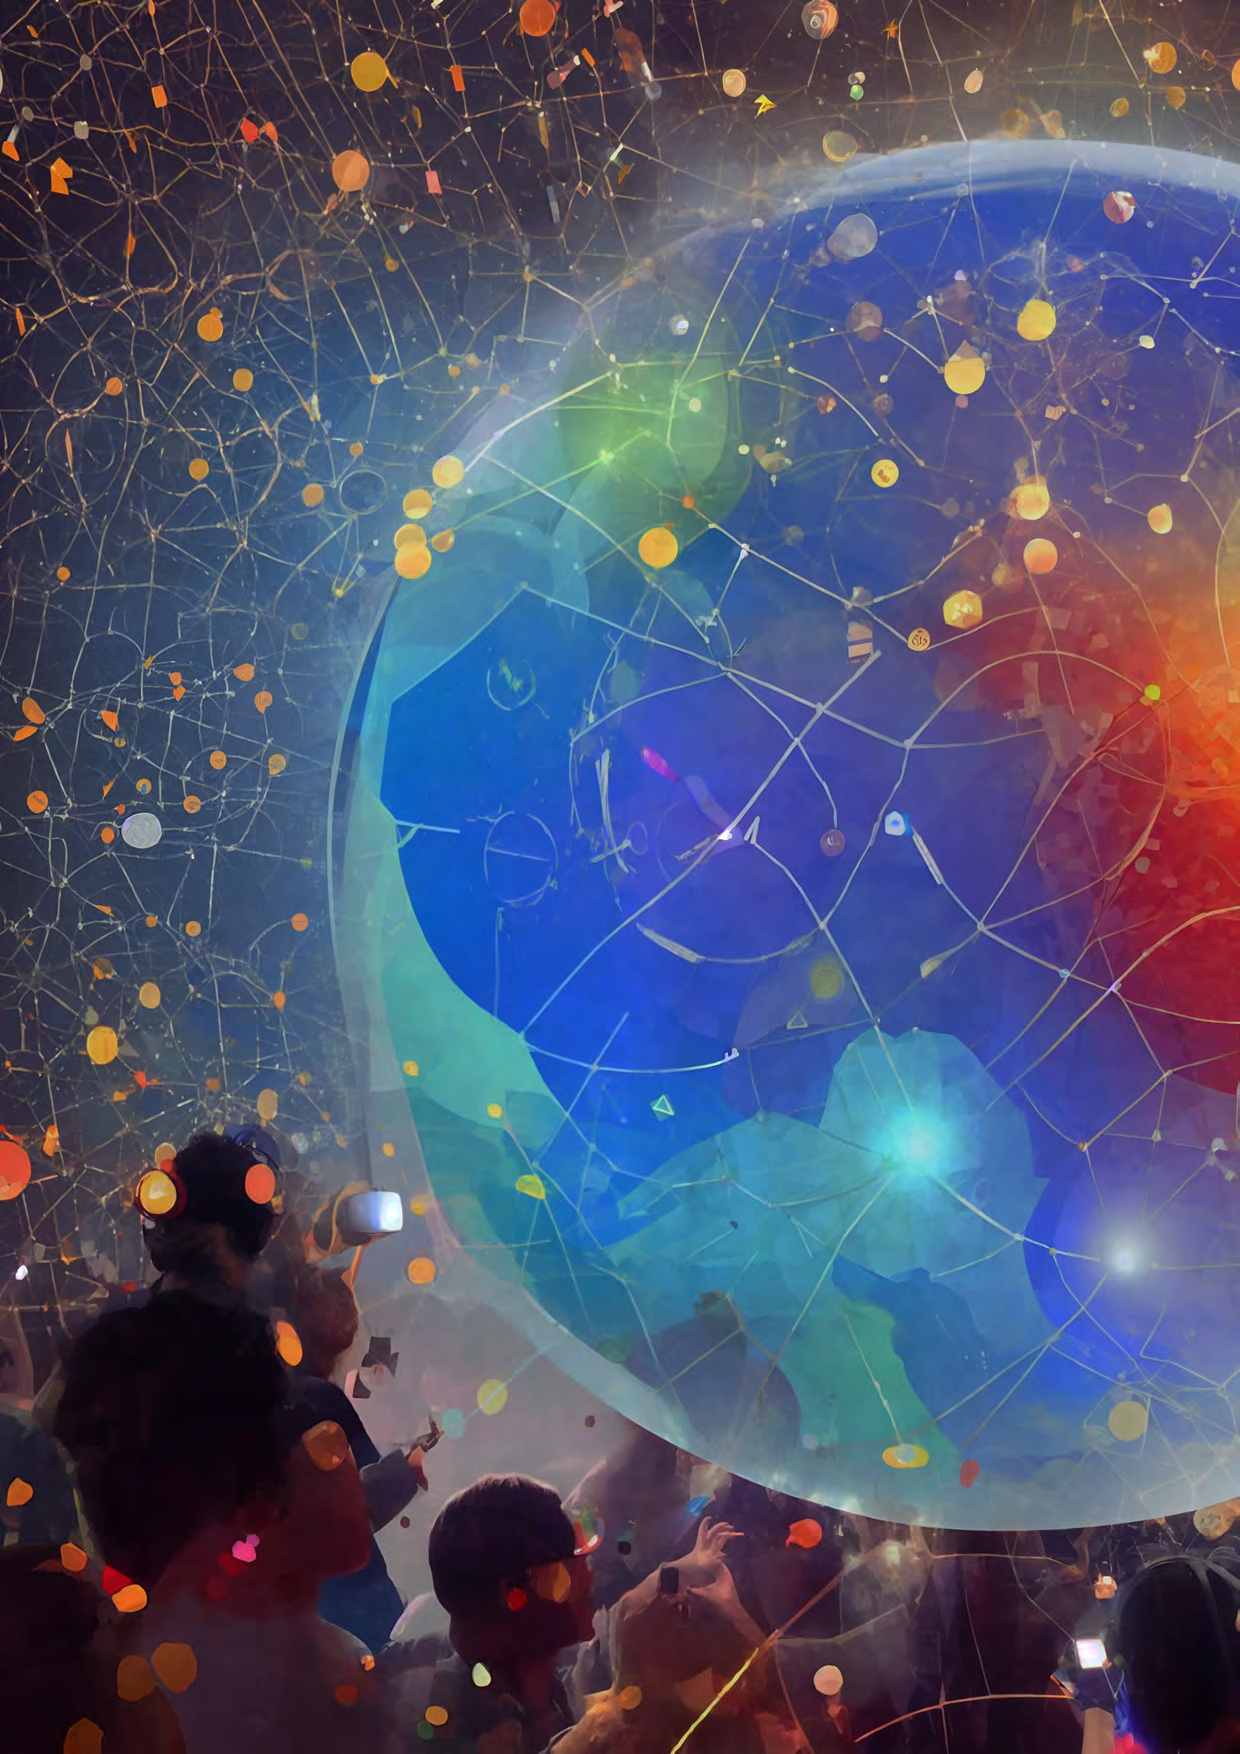
\includegraphics[width=\paperwidth]{background.pdf}} % Code to output the background image, which should be the same dimensions as the paper to fill the page entirely; leave empty for no background image
	{ % Title(s) and author(s)
		\centering\sffamily % Font styling
		{\Huge\bfseries Money in Metaverses\par} % Book title
		\vspace{16pt} % Vertical whitespace
		{\LARGE Bitcoin and stablecoins in  social XR\\a draft product roadmap\par}  % Subtitle
		\vspace{24pt} % Vertical whitespace
		{\large \textbf{John O'Hare, Allen Fairchild, and Umran Ali}\par} % Author name
	}

%----------------------------------------------------------------------------------------
%	COPYRIGHT PAGE
%----------------------------------------------------------------------------------------

\thispagestyle{empty} % Suppress headers and footers on this page

~\vfill % Push the text down to the bottom of the page

\noindent \href{https://creativecommons.org/publicdomain/zero/1.0/}{No Copyright}\\ 2022 John O'Hare \& Allen Fairchild \& Umran Ali\\ % Copyright notice

\noindent \textsc{Published by j.ohare@salford.ac.uk for the Cyber Foundry Programme at The University of Salford}\\ % Publisher

\noindent \textsc{\href{https://raw.githubusercontent.com/GMCyberFoundry/Metaverse/main/Paper/metaverseBTC.pdf}{Raw GitHub hyperlink}}\\ % URL

\noindent The person who associated a work with this deed has dedicated the work to the public domain by waiving all of his or her rights to the work worldwide under copyright law, including all related and neighboring rights, to the extent allowed by law.\\
You can copy, modify, distribute and perform the work, even for commercial purposes, all without asking permission. See Other Information below.\\
This license is acceptable for Free Cultural Works.
Other Information\\
In no way are the patent or trademark rights of any person affected by CC0, nor are the rights that other persons may have in the work or in how the work is used, such as publicity or privacy rights.\\
Unless expressly stated otherwise, the person who associated a work with this deed makes no warranties about the work, and disclaims liability for all uses of the work, to the fullest extent permitted by applicable law.\\
When using or citing the work, you should not imply endorsement by the author or the affirmer.\\
\noindent This work was supported by the European Regional Development Fund (ERDF) GM Cyber Foundry Project (15R18P02426)\\

\noindent \textit{First printing, March 2022} % Printing/edition date

%----------------------------------------------------------------------------------------
%	TABLE OF CONTENTS
%----------------------------------------------------------------------------------------

\pagestyle{empty} % Disable headers and footers for the following pages

\tableofcontents % Output the table of contents

\listoffigures % Output the list of figures, comment or remove this command if not required

\listoftables % Output the list of tables, comment or remove this command if not required

\pagestyle{fancy} % Enable default headers and footers again

\cleardoublepage % Start the following content on a new page

%----------------------------------------------------------------------------------------
%	PART
%----------------------------------------------------------------------------------------

\part{State of the art and proposal}

%----------------------------------------------------------------------------------------
%	SECTIONING EXAMPLES CHAPTER
%----------------------------------------------------------------------------------------

\chapterimage{orange2.jpg} % Chapter heading image
\chapterspaceabove{6.75cm} % Whitespace from the top of the page to the chapter title on chapter pages
\chapterspacebelow{7.25cm} % Amount of vertical whitespace from the top margin to the start of the text on chapter pages

%------------------------------------------------

\section{Conflict of interest statements}
\input{conflicts}
\chapter{Introduction}
\section{Overview}
Money is a social construct, like trust. Both are very important and ephemeral things, and are being tested in a global digital world.  We are a long way from the village structures in which we evolved. We are now expected to casually adapt to the efficiencies promised by teams working in global mixed reality. This chaotic and intangible mix of value, trust, and socialisation is not well understood.\par
We wanted to explore exciting new developments in the transmission of value, and trust, in `digital society'. The problem is that each of these topics alone are enormously complex, and the intersections seem to be more so. We have been researching the current state-of-the-art, and the emerging consensus narrative, to try to figure out how the collision of these technologies might serve our virtual production workflows (Figure \ref{fig:pathway}).\par
Over the course of a couple of years the focus of the work has developed, and refined. The toolkit as it stands supports inclusive human creativity and economic exchange, especially for emerging markets and the global south. There is a huge proportion of human creativity currently excluded from media production pipelines due to gatekeepers of knowledge, access to identity proofs, and financial infrastructure that is taken for granted in the richer nations. This inclusion will be accomplished for the most part through integration of open source machine learning and AI tools, but this field quite new, and that part of the work is under developed.\par

\textbf{\hyperref[sec:tldr]{If at this stage you want to skip straight to the TL;DR for the whole book then click this bold text}.}\par
\begin{figure}
  \centering
   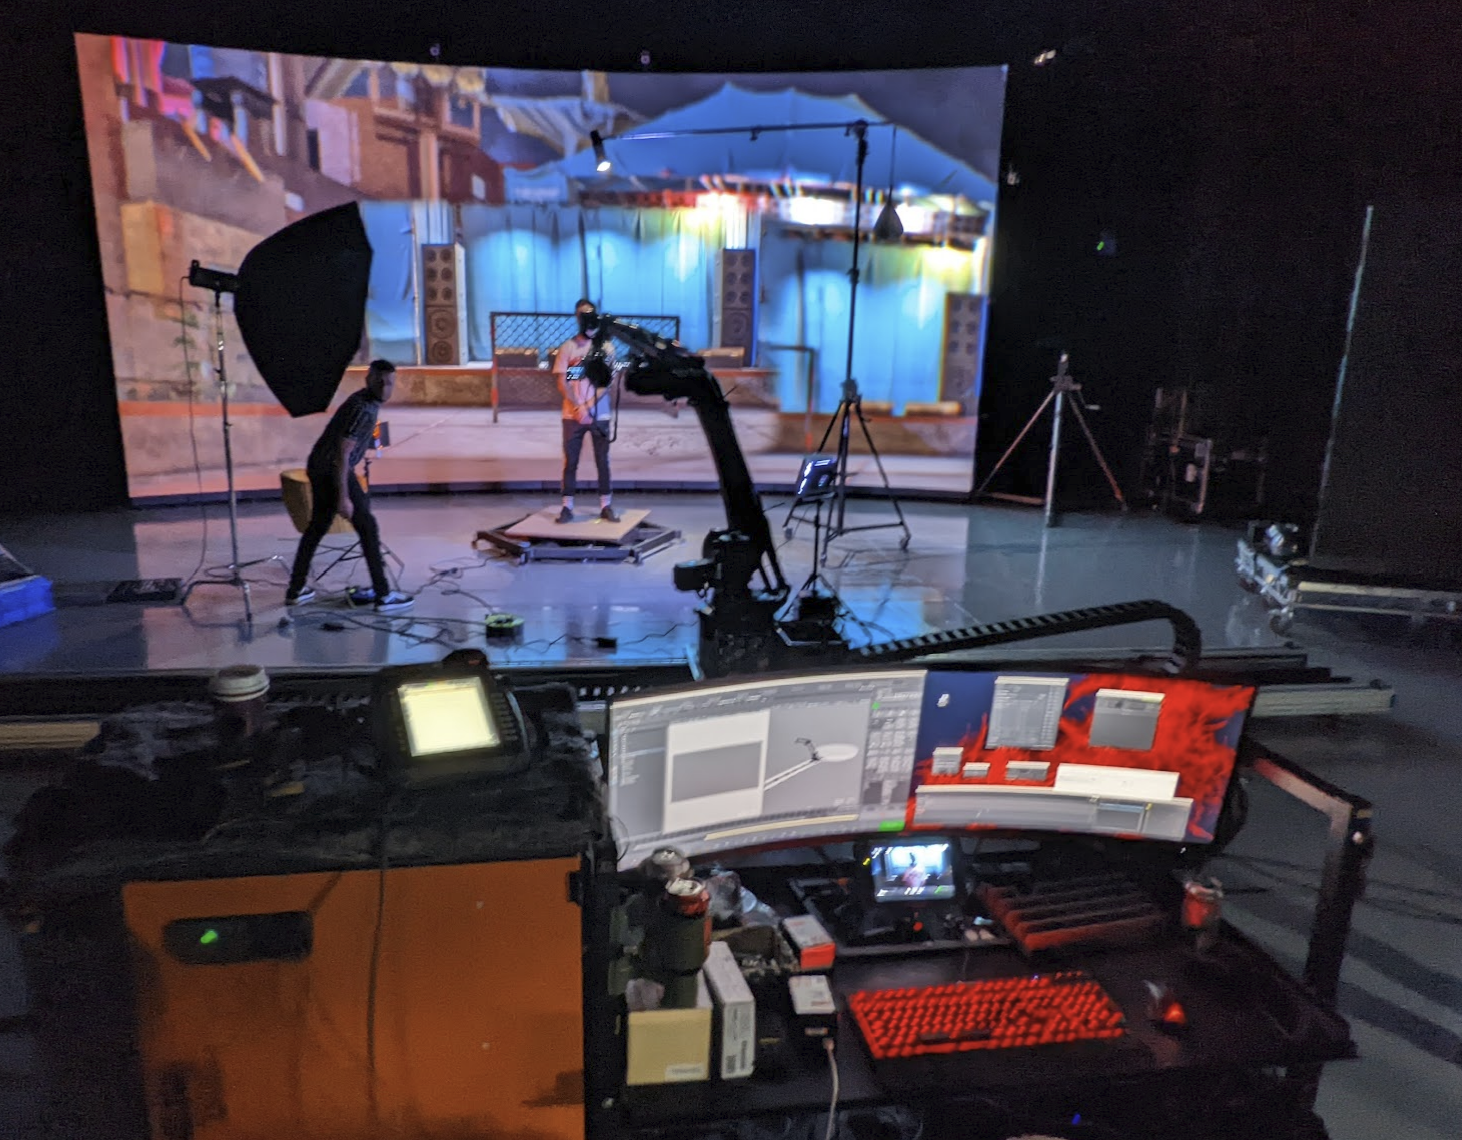
\includegraphics[width=\linewidth]{pathway}
 \caption{\href{https://www.pathwayxr.studio/}{Pathway XR virtual production}}
    \label{fig:pathway}
\end{figure}
Cybersecurity is top of the list of concerns in the \href{https://digital-strategy.ec.europa.eu/en/policies}{EU digital society strategy}, just ahead of digital inclusion, so we started out with security best practices in mind, and we tried to end the investigation with inclusion. We aim to support small and especially developing companies in our sector, giving them a foot in the door on a global stage, without their costs spiralling? \par
Fortunately, we discovered a wealth of carefully crafted open source tools which can support this. We have tried to assemble them cogently, to deliver an open source kit for experimentation, to curious technically minded SMEs outside of Pathway, and we have applied our own security knowledge on top of an already top class set of tools. It’s certainly not production ready, but it's good enough to commit small amounts of money into, and collaboration with Pathway is welcomed.\par
Whilst researching, it seemed that every door we opened was full of interesting and useful treats. What was supposed to be a short technical paper quickly became a 200-page book, and a deployable virtual machine stack, with a dozen different open source components in it. \par
This book supports the software stack, which supports anyone who thinks this material might be useful. Below is a précis of the chapters of the book, which will hopefully give an insight into what ``this stuff'' is. The reader can decide to download the book and the system ``How To'' guide. All of it is open source, all of it can be contributed to on GitHub, all of it will be developed forward, and none of it is really finished yet.\par
Chapter 1 starts with an introduction to the book which is about value transmission, with distributed trust, in global digital society and mixed reality systems. \par
Next is a summary of Web3, as it stands right now. Web3 is a complex term that is cropping up far more in the technical press, so we wanted explain what it might mean. Honestly, it’s still pretty confusing. There are a bunch of legacy explanations which are Web3.0 (note the `0' there), but these are withering on the vine. Then there’s the new VC funded, super hyped, and potentially useless Web3 incarnations, which again cover a slew of intersecting technologies. Note they dropped the zero to reboot the brand! This doesn’t mean there’s nothing to see here. The astonishing amount of \href{https://mirror.xyz/tr3butor.eth/AlZPMq_syymAoi8M1VVb2xES9Twj1OeetJbEE7EWhiw}{money and developer talent}, and the clear market hunger for things like NFTs (non-fungible tokens) suggest that there’s a future for Web3, it’s just really unclear if this is inherently valuable or just hype.\par
In the next chapter we took a look at blockchain, which is very intersectional with Web3. Even on its own this is a complex emergent set of disciplines. \par
The blockchain chapter was especially interesting to research. It turns out there’s a \textit{lot} of ways to get this technology wrong. Even very appealing options on paper, turn out to have very shaky foundations. There are valuable things here, but given the complexity and scope, we decided to focus on the most promising of the technology stacks; the Bitcoin network.\par
Even Bitcoin isn’t just Bitcoin any more. It’s a swarm of open source tools which can (in theory) accomplish a great many things. These newer, ancillary elements to Bitcoin, are emergent right now. Some of them won’t be around until next year, and it’s questionable whether they will even work out. With that said we aren't convinced by the value proposition of of Ethereum, and there’s enough Bitcoin tooling for us to cherry pick useful components. We map those forward into our metaverse product.\par
%It seems possible that the features which are important to Web3, can also (potentially) arise from the Bitcoin technology that we think most secure. This was somewhat unexpected, so we started mapping that over too.\par
The next chapter is about Money. In expanding our research on Bitcoin, we found that it’s impossible to think about the tech without opening up a whole line of questions about money itself. This is fine because we set out to look at global value transfer for business. It’s not a trivial subject though, and this section tries to overview why value and Bitcoin are so enmeshed, then what other options there might be in the end (because Bitcoin has kicked off a whole slew of global adoption outside of itself).\par
The distributed identity management, and trust chapter follows. Identity management is important for digital society and potentially crucial to metaverse applications which have a value transaction layer. It’s not an easy section to write about, because there’s a lot of research, it’s not our field, and finding the value to SMEs has actually been very difficult. It's by no means clear that blockchain is the right tool for this component, and newer cryptographic products are emerging.\par %This section is likely to be overhauled a few times in the coming months as we settle on technologies that we believe are simple and secure enough.\par
In chapter 7 we take another look at NFTs. It’s impossible to ignore this stuff now. It’s fundamentally a bit broken, but there are probably use cases, and the money and development attention it’s getting are incredible. We try to navigate our hypothetical virtual production partners through this as best we can. \par %It’s not that we didn’t understand it completely, just that the tech moves so very fast that it’s impossible to even describe what’s going on accurately at any given point. \par
We’re actually pretty excited about future versions of `digital assets', based around Bitcoin, because that allows us to keep just one software stack, minimising the threat surface. We’ve mapped that forward into the open source tools that we recommend.\par
Chapter 8 is a big one for us as it’s our research area prior to opening up the Bitcoin box(es). Metaverse, or at least one of the current definitions of metaverse, is just social interaction in mixed reality (VR/AR/XR). We’ve been studying that for decades, so this section is more academic and tried to boil down what we think is most important. The choices we made here guided us toward the selection of free and open source metaverse software.\par
We also take a look at the other definitions of `metaverse' which are doing the rounds on the web, try to unpick which is which, and what they are for, and attempt to weave back together the best of both. This ends up looking a bit like the Venn in Figure \ref{fig:landscapevenn}, where we have transmission of provable identity, non-fungible tokens bearing value or data, distributed files, actual money (including micropayments) and a social layer based on our best knowledge about mixed reality. In the end we abandon the word metaverse and settle on `digital society' as our preferred term.\par
It's exceptionally fortunate timing for this book that the UK government has signalled enthusiasm for so called `stablecoins' at the same time that the Bitcoin network is being upgraded to transmit these GBP equivalent tokens around. This gives us a very good idea what it is we can build into our application stack.\par 
Past this stage in the book we get into the murky and half developed tail end, where we’re interfacing with our design choices, and the stack which can be deployed into the cloud.
\begin{figure*}[ht]\centering % Using 
	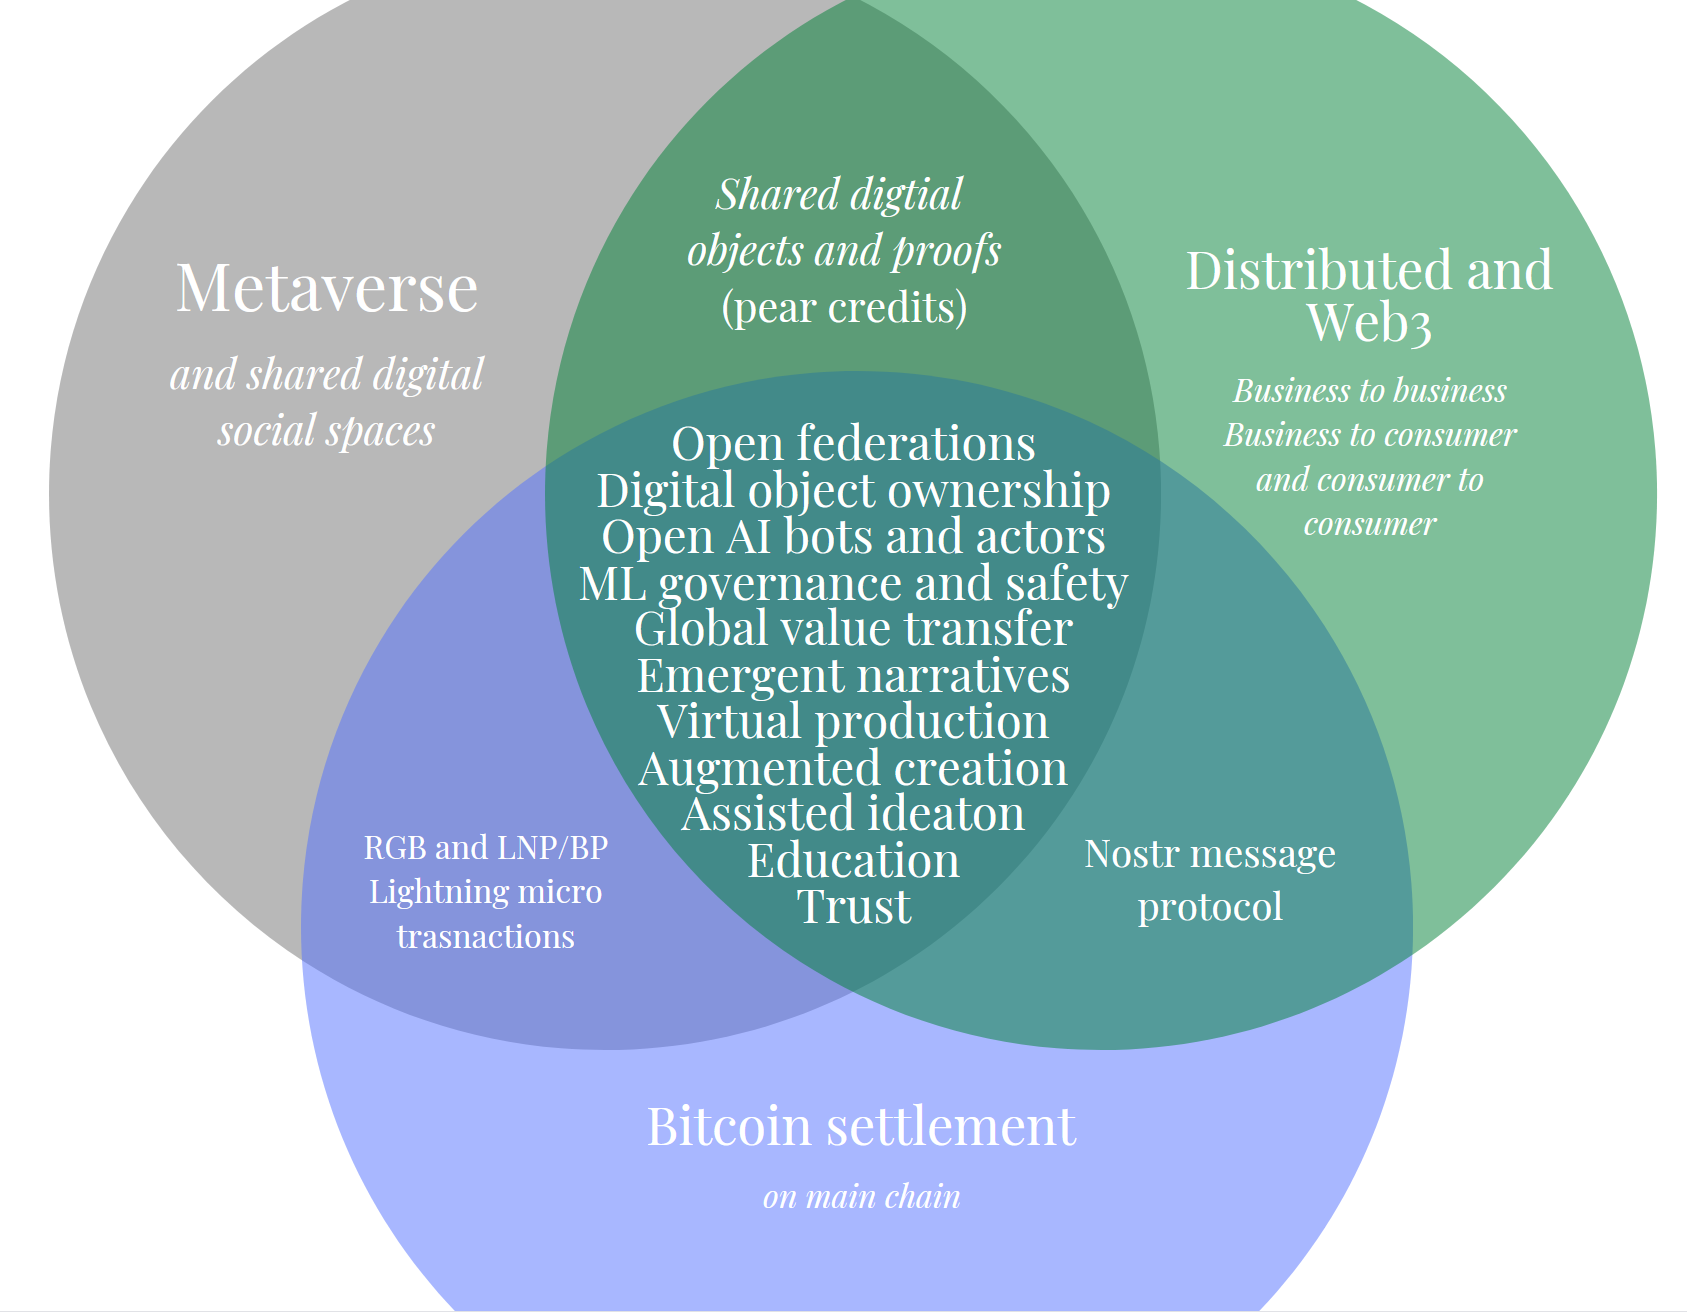
\includegraphics[width=\linewidth]{landscapevenn}
	\caption{Web 3, Metaverse, and Bitcoin are intersectional technologies.}
	\label{fig:landscapevenn}
\end{figure*}


\section{Introduction}
This document presents a high level view of technologies and their potential within the emergent Web3 and metaverse narrative, focusing around the transmission of value within and across such global networks, with a further focus on the Bitcoin monetary network. It was written to organise the thoughts of the authors, who were unfamiliar with Bitcoin technologies until recently.\par
As adoption of these technologies increases it will be necessary for people, and AI actors, to pass economic value between themselves. These `goods and services' interactions, within the virtual social spaces should be underpinned by a trust system, which scales globally and presents low friction. Current secure international payment rails are poorly suited to such interactions; indeed it is likely with legacy systems, that parties would be forced to leave the metaverse application, and instead navigate their banking applications to exchange value with overseas entities in a secure fashion. This might conceivably take several days.\par 
Fortunately, the whole landscape of money and \href{https://www.omfif.org/futureofpayments2021/}{value transfer is changing}. Huge global financial players are entering the space. HSBC have \href{https://sandboxgame.medium.com/hsbc-to-become-the-first-global-financial-services-provider-to-enter-the-sandbox-c066e4f48163}{just bought} metaverse `land' in The Sandbox, JP Morgan have \href{https://www.forbes.com/sites/ronshevlin/2022/02/16/jpmorgan-opens-a-bank-branch-in-the-metaverse-but-its-not-for-what-you-think-its-for/?sh=2fbd1e90158d}{opened a `lounge'} in another. The worlds largest hedge fund Bridgewater is stepping into \href{https://uk.finance.yahoo.com/news/bitcoin-latest-price-crypto-ray-dalio-bridgewater-investment-fund-ethereum-094946686.html}{acquisition of digital assets}, and the world's largest pension fund manager Blackrock is adding these asset to their management engine (which manages tens of trillions of dollars). Fidelity asset management are about to add \href{https://www.wsj.com/articles/fidelity-to-allow-retirement-savers-to-put-bitcoin-in-401-k-accounts-11650945661}{Bitcoin to their pension plans} and are offering a \href{}{dedicated metaverse tradable fund}, while \href{https://www.citivelocity.com/citigps/metaverse-and-money/}{Citigroup have a minisite} dedicated to ``Metaverse and Money''. The front page of Goldman Sachs recently says it all (Figure \ref{fig:goldmanFront}).\par
\begin{figure}[ht]\centering % Using \begin{figure*} makes the figure take up the entire width of the page
	\includegraphics[width=0.5\linewidth]{goldmanFront}
	\caption{The landing page of global\\financial giant Goldman Sachs shows the hype.}
	\label{fig:goldmanFront}
\end{figure}
Of their recent investments KPMG global said: \textit{``We've invested in a strong cryptoassets practice and we will continue to enhance and build on our capabilities across Decentralized Finance (DeFi), Non-Fungible Tokens (NFTs) and the Metaverse, to name a few''}.\par
It's possible that for such organisations it makes better business sense to take a punt on hype bubbles like this, than to do a proper due diligence with a team of internal staff who understand their business. These endorsements should be taken with a large pinch of salt. As \href{https://newsletter.fintechtakes.com/p/metaverse-branches?s=r}{Alex Johnson says}: \textit{``At some point in the future, it’s possible that the digital worlds being built today will have aggregated sufficient user attention and engagement that financial services companies will need to invest in the metaverse as an acquisition and customer service channel. But we’re not there yet. Until the metaverse is a little less empty, resist the temptation to colonize it with branches and billboards.''}\par
Meanwhile, Meta (ex Facebook) are launching their own \href{https://archive.ph/coyp2}{META Web3 and metaverse} token (after abandoning Libre, their global cryptocurrency), and \href{https://www.cnbc.com/2022/05/06/googles-cloud-group-forms-web3-product-and-engineering-team.html}{Google} have \href{https://blog.youtube/inside-youtube/innovations-for-2022-at-youtube/}{recently blogged}: \textit{``Web3 also opens up new opportunities for creators. We believe new technologies like blockchain and NFTs can allow creators to build deeper relationships with their fans. Together, they'll be able to collaborate on new projects and make money in ways not previously possible. For example, giving a verifiable way for fans to own unique videos, photos, art, and even experiences from their favourite creators could be a compelling prospect for creators and their audiences. There's a lot to consider in making sure we approach these new technologies responsibly, but we think there's incredible potential as well. Finally, we couldn't have a piece about innovation without touching on the metaverse! We're thinking big about how to make viewing more immersive. ''}\par
It's already the case that the recent bubble of \href{https://www.forbes.com/sites/paultassi/2022/03/10/interest-in-nfts-and-the-metaverse-is-falling-fast/?}{hype is dwindling}, but the enormous investment into teams and startups will potentially bear fruit in the next couple of years, and this perhaps has implications for small and medium-sized enterprises (SMEs). \par
In the UK the government has stated it's ambition to be a \href{https://www.gov.uk/government/news/government-sets-out-plan-to-make-uk-a-global-cryptoasset-technology-hub}{global cryptoasset technology hub}, and announced plans for the Royal Mint to issue a (novelty) NFT. Like the assertion by major global businesses it is too early to tell how `sticky' these claims are.\par
With all this attention it seems timely to explore the potential of recent technologies, which can address metaverse interactions in \textit{business to business} (B2B), \textit{business to customer} (B2C), and the newer C2C (social commerce; \textit{creator to consumer, customer to customer, consumer to consumer\cite{jones2008trust})}. Figure \ref{fig:landscapevenn} demonstrates how some of these domains intersect.\par
This book seeks to overview and explain the available open source technologies. It supports an open source \href{https://github.com/GMCyberFoundry/Metaverse}{github repository} which enables SMEs to access these emergent platforms and ecosystems. It aims to build toward a minimum viable product for trust minimised transfer of value within a social immersive space.\par
Referencing is in two styles; academic works and books are numeric, while opinion pieces, gray statistics, and pertinent news articles are hyperlinked from the text. This hybrid style yields about twice the citation density of a normal PhD thesis, which is a lot. For this reason the normal blue hyperlink colour was eschewed in favour of a more aesthetic ``gray''. There is also a version of the PDF which complies with accessibility best practice if this is a problem.  \par 
\subsection{Notes on progress}
\textbf{This version of the book is ``minimally complete''. The real interesting work of combining the primitives into a new direction for integration of Bitcoin and VR is just beginning. We are now inviting the wider community to submit pull requests into github as contributors. It's been a useful document creation process to form our thoughts, and it's enough to bring a reader up to ``the state of the art'' if all of the thousand  links and papers are considered. It's an open ended project though.}\

\begin{figure*}[ht]\centering % Using \begin{figure*} makes the figure take up the entire width of the page
	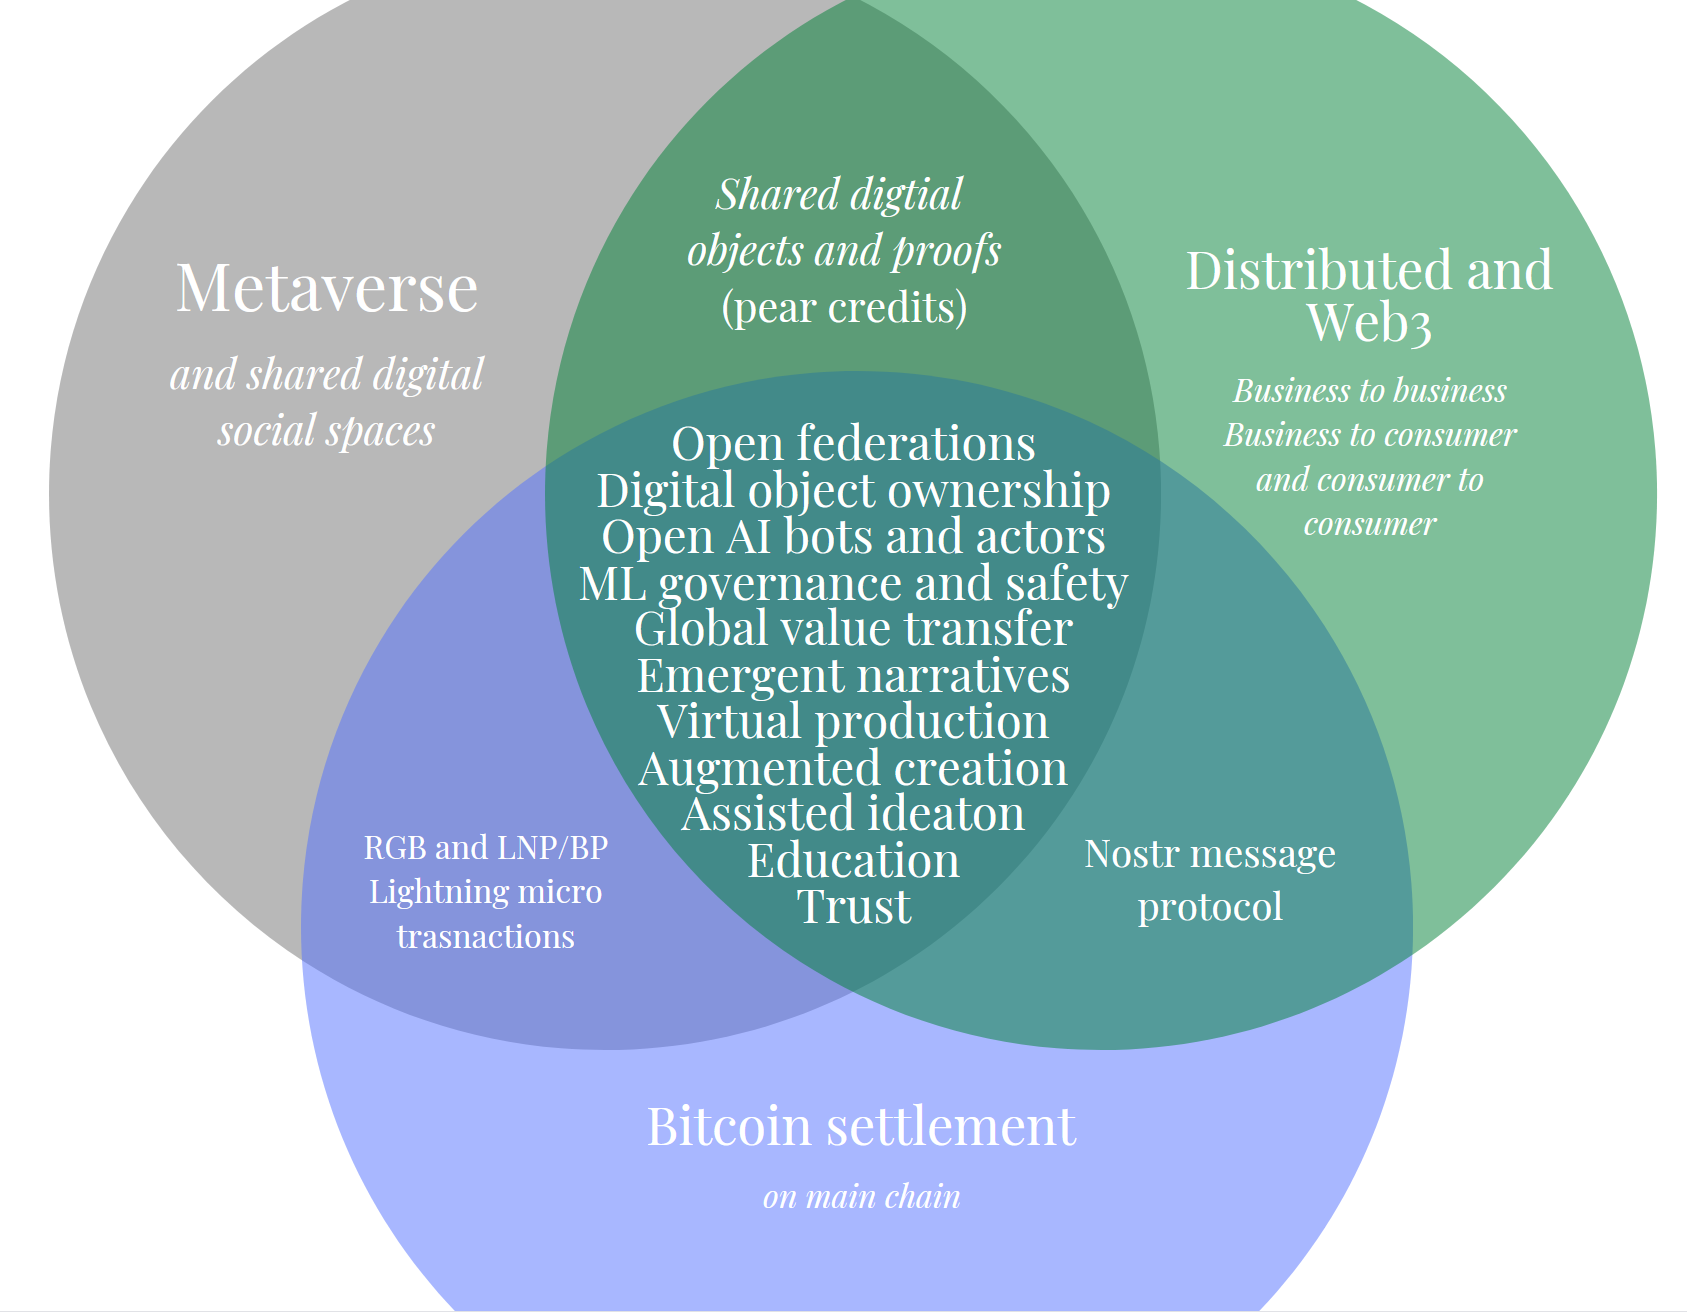
\includegraphics[width=\linewidth]{landscapevenn}
	\caption{Web 3, Metaverse, and Bitcoin are inter-sectional technologies.}
	\label{fig:landscapevenn}
\end{figure*}
\chapter{Decentralisation\& Web3}
When this chapter was first started in early 2022 `Web3' was at the peak of it's hype. Web3 is still a rapidly evolving set of technologies and specifications, which are drifting further from their origin. Decentralised web is perhaps a more useful name.%, but focus in this section will be on the evolution of the popularised term Web3. 
\section{Semantic web}
The ``semantic web'' definition of Web3.0 has been somewhat overhauled by other innovations in decentralised internet technologies, now evolving toward the slightly different Web3 moniker. Tim Berners Lee (of WWW fame) first mentioned the semantic web in 1999 \cite{semanticWeb}.\par
``I have a dream for the Web [in which computers] become capable of analyzing all the data on the Web – the content, links, and transactions between people and computers. A "Semantic Web", which makes this possible, has yet to emerge, but when it does, the day-to-day mechanisms of trade, bureaucracy and our daily lives will be handled by machines talking to machines. The "intelligent agents" people have touted for ages will finally materialize.''\par
Attention developed around three core themes, ubiquitous availability and searchability of data, intelligent search assistants, and highly available end points such as phones, and `internet of things' devices. This is certainly manifesting in home devices, but few people think of this as a Web3 revolution. 
\begin{comment}
The framework can be seen in Figure \ref{fig:semanticWebStack}.\par
\begin{figure}
  \centering
    \includegraphics[width=\linewidth]{semanticWebStack}
  \caption{\href{https://en.wikipedia.org/wiki/Semantic_Web_Stack}{Semantic Web Stack} [CC0 image]}
  \label{fig:semanticWebStack}
\end{figure}
\end{comment}
Since ratification of the standards by the \href{https://www.w3.org/standards/semanticweb/}{World Wide Web (W3C) consortium} it seems that their imperative toward decentralisation has become lost. Instead, it can be seen that Facebook, Amazon, Google, and Apple have a harmful oligopoly on users data \cite{costigan2018world}. This is at odds with Berners-Lee's vision, and he has recently \href{https://thenextweb.com/news/web-inventor-tim-berners-lee-screw-web3-my-decentralized-internet-doesnt-need-blockchain/}{spoken out about this discrepancy}. \par
It is worth taking a look at his software implementation called \href{https://solidproject.org}{Solid}, which is far more mindful of the sovereignty of user data.\par
``Solid is an exciting new project led by Prof. Tim Berners-Lee, inventor of the World Wide Web, taking place at MIT. The project aims to radically change the way Web applications work today, resulting in true data ownership as well as improved privacy. Solid (derived from "social linked data") is a proposed set of conventions and tools for building decentralized social applications based on Linked Data principles. Solid is modular and extensible and it relies as much as possible on existing W3C standards and protocols.'' \par
Excitement around this kind of differentiated trust model, hinted at in ubiquitous availability of data (and implemented explicitly in Solid), has led to exploration of different paths by cryptographers, and this will be described later. For instance, one of the main developers of Solid, Melvin Carvelho, is now a lead developer at Nostr, another very interesting option which will be described later. This technology space is prolific, but still comparatively young and small.\par
\section{Spatial web}
``The Spatial Web'', a blurring of the boundaries between digital and geospatial physical objects, seems to have developed from the strands in the original W3C scope around devices in the real world. It has been concentrating around AR and VR but is being marketed and amplified with the same references to availability of data (See Figure \ref{fig:deloitteSpatial} from a Deloitte accounting report). This too is finding little traction in practice, though obviously the component technologies continue to enjoy rapid development. Nonetheless, this interpretation of Web3 becomes valuable when examining Metaverse later.\par
\begin{figure}
  \centering
    \includegraphics[width=\linewidth]{deloitteweb3}
  \caption{\href{https://www2.deloitte.com/us/en/insights/topics/digital-transformation/web-3-0-technologies-in-business.html}{Deloitte Spatial Web Overview} Reused with permission.}
  \label{fig:deloitteSpatial}
\end{figure}
\section{Web3}
More recently Web3 is \href{https://trends.google.com/trends/explore?date=all&q=web3}{being touted} as a way to connect content creators directly to content consumers, without centralised companies acting as gatekeepers of the data. It implies that all users have a cryptographic key management system, to which they attach metadata, that they make requirements of peers with whom they communicate, and that they maintain trust `scores' with peers.\par
It seems likely that this new model is less driven by a market need, and more by the high availability of tools which allow this to happen (the ecosystems described later). Add to this a social response to the \href{https://finance.yahoo.com/news/meta-facebook-worst-company-of-the-year-yahoo-finance-165345819.html}{collapse in trust of companies such as Facebook} and other \href{https://reb00ted.org/tech/20220727-end-of-social-networking/}{social media platforms} (Figure \ref{fig:trustbarometer}). There is perhaps a wish by consumers to pass more of the economic incentive to content creators, without the `rent seeking' layer afforded by businesses, and a healthy dose of mania driven market speculation. 

\begin{figure}
  \centering
    \includegraphics[width=\linewidth]{c-a-e}
  \caption{\href{https://www.edelman.com/trust/2020-trust-barometer}{Edelman 2020 trust barometer} [rights requested]}
  \label{fig:trustbarometer}
\end{figure}
\subsection{Emerging consensus}
It's possible to frame Web3 as a hugely complex and inefficient digital rights management system (DRM). DRM is something that users of the internet are increasingly familiar and comfortable with. It's somewhat debatable whether decentralising this is worthwhile. The thesis of the developers of the technology seems to be that without it, control of `value' will accrete over time, to one or more hegemonic controlling entities. It's a strong argument, but there is a \href{https://moxie.org/2022/01/07/web3-first-impressions.html}{substantial counter argument} emerging that users just don't want this stuff. The nervousness of legislators in the USA to the attempt by Facebook/Meta to enter this peer-to-peer value transmission space is telling in terms of the perception of who is driving Web3.\par
At the end of 2021 and the beginning of 2022 there is much furore on the internet over what Web3 might be, and who it `serves'. 
Enthusiasts feel that products such as \href{https://blog.spruceid.com/sign-in-with-ethereum-is-a-game-changer-part-1/}{Sign-In with Ethereum} (EIP-4361) will give users choice over their data sovereignty, and a meme to this effect is seen in Figure \ref{fig:web1web2web3}. In practice though users are expecting to use badly written, buggy, economically vulnerable `crypto' wallets to log into websites. The quality of this wallet software is improving of late with the so called ``wallet wars'' seeing commerce grade offerings from Coinbase and shares platform `Robinhood'. These two companies alone have over 100 million users. It's likely that these wallets will evolve to offer the full spectrum of Web3 functionality. With that said it doesn't seem to make much sense yet on the face of it. There are in fact examples of the technology completely failing at censorship resistance. Popular `Web3' browser extension Metamask and NFT platform Opensea have both \href{https://www.forbes.com/sites/stevenehrlich/2022/03/03/iranian-venezuela-users-abruptly-dropped-from-major-crypto-platforms-as-russian-sanctions-grow/?sh=22bcabc470b0}{recently banned countries} in response to global sanction pressure. This failure to meaningfully decentralise will be explored further in the distributed identity section. \par
\begin{figure}
  \centering
   \includegraphics[width=\linewidth]{web1web2web3}
 \caption{A meme showing differing approached to logging in on a website.}
 \label{fig:web1web2web3}
\end{figure}
The current hype cycle is ignoring the legacy definitions described above and instead focusing almost exclusively on Ethereum based peer-to-peer projects (more on these later). It can be seen that the description is somewhat in the eye of the beholder.\par
This new hyped push for Web3 is being driven by enormous venture capital investment. A16Z are a \href{https://a16z.com/2022/01/07/9b-to-build-the-future/}{major player} in this new landscape and have released their \href{https://a16z.com/2022/01/07/how-to-build-a-better-internet-10-principles-for-world-leaders-shaping-the-future-of-web3/}{ten principles} for emergent Web3. 
\begin{itemize}
\item Establish a clear vision to foster decentralized digital infrastructure
\item Embrace multi-stakeholder approaches to governance and regulation
\item Create targeted, risk-calibrated oversight regimes for different web3 activities
\item Foster innovation with composability, open source code, and the power of open communities
\item Broaden access to the economic benefits of the innovation economy
\item Unlock the potential of DAOs
\item Deploy web3 to further sustainability goals
\item Embrace the role of well-regulated stablecoins in financial inclusion and innovation
\item Collaborate with other nations to harmonize standards and regulatory frameworks
\item Provide clear, fair tax rules for the reporting of digital assets, and leverage technical solutions for tax compliance
\end{itemize}
This list seems targeted toward the coming regulatory landscape, and could be considered at odds with the original tenants of an organically emergent, decentralised internet. Indeed principles such as `furthering sustainability goals' seem downright incongruous. The community they claim to wish to support here are openly critical of these major institutional players and their motives, with even more pointed criticisms \href{https://www.profgalloway.com/web3/}{coming from outside of the Web3}. This book and lab steer well clear of these companies and their applications.\par
Dante Disparte, chief strategy officer of `Circle' venture capital, said in testimony to a US senate hearing; that Web 1 was `read', Web 2 was `read write', and that Web 3 will `read write own'. The important takeaway here is not so much this oft quoted elevator pitch for Web3, but the fact that legislative bodies now consider this technology a force which they need to be aware of and \href{https://a16z.com/2021/12/17/prediction-for-the-new-year-a-web3-midterm/}{potentially contend with}.\par
Jeremy Allaire, again of Circle', talks about the recent legislative order in the USA as follows:
\textit{``this is a watershed moment for crypto, digital assets, and Web 3, akin to the 1996/1997 whole of government wakeup to the commercial internet. The U.S. seems to be taking on the reality that digital assets represent one of the most significant technologies and infrastructures for the 21st century; it's rewarding to see this from the WH after so many of us have been making the case for 9+ years.''}\par
We will see in the following chapters that participation in this new Web3 is contingent on owning cryptocurrencies. \href{https://www.finder.com/uk/cryptocurrency-statistics}{It's estimated} that about 6\% of people in the UK own some cryptocurrency, with skews to both younger demographics, and smaller holdings. The legislative landscape in the UK is comparatively strict with strong ``know your customer / anti money laundering'' (KYC/AML) data collection \href{https://www.gov.uk/guidance/money-laundering-regulations-your-responsibilities}{mandated in law}. Users of UK exchanges must provide a great deal of personal financial information, and undertake to prove that the wallets they are withdrawing to are their own. From the perspective of the UK SME it seems this seriously limits the potential audience for new products. Europe meanwhile has recently voted through even more restrictive regulation, applying the ``\href{https://www.europarl.europa.eu/legislative-train/theme-an-economy-that-works-for-people/file-revision-of-the-regulation-on-transfers-of-funds}{transfer of funds regulation}'' to all transactions coming out of exchanges, enforcing a database of all addresses between companies, and reporting transactions above 1000 Euros to authorities. They have narrowly avoided enforcing KYC on all transfers to private wallets. The \href{https://www.consilium.europa.eu/en/press/press-releases/2022/06/30/digital-finance-agreement-reached-on-european-crypto-assets-regulation-mica/}{``Markets in Crypto Assets (MiCA)} legislation is an onerous overhead that will likely make it impossible for smaller businesses in the sector to operate within the EU. This is still short of the ban that they have \href{https://netzpolitik.org/2022/climate-measures-behind-closed-doors-eu-officials-talk-about-banning-bitcoin/}{discussed in private}. It seems that this EU position has prompted the UK government to seize the potential competitive advantage offered, and there will be more on this later.\par
%Many of the mentioned components here will be described later in the book. The suggestion is that this is happening regardless of a decent use case or definition.\par
It's a complex evolving narrative, and clearly contradictions are common. Right now there seems little appeal for stepping into Web3. Into the confusion, this book advances a narrow take, and toolset, which might extract some value from the technologies, while maintaining a low barrier to entry.\par 
\begin{comment}
\section{Example applications}
It's handy here to get a feel for what this looks like. These aren't things that this book wishes to contribute to, or even have a firm opinion on, they're just representative of current activity in the decentralised web space.
\subsection{Podcasting2.0}
\href{https://medium.com/@everywheretrip/an-introduction-to-podcasting-2-0-3c4f61ea17f4}{Podcasting 2.0} leverages \href{https://www.rssboard.org/rss-specification}{RSS} (the original dissemination system for podcasts) and the Bitcoin Lightning network, to enable so-called `\href{https://www.youtube.com/watch?v=NO1aDZ6L4NQ&t=1123s}{value for value}' broadcasting. Subscribers use one of a variety of apps to stream micro-transactions of Bitcoin directly to the content creators as they listen to the podcast. No intermediate business takes a cut. Some variation on this model exists, such as John Carvalho's crowd funded podcast ``The Biz'' which progressively unlocks more minutes for everyone based on \href{https://thebiz.pro/about#crowdwall}{crowd funded donations}.
\subsection{Crowd funding}
At time of writing a \href{https://www.constitutiondao.com/}{crowd funding initiative} based around a digital decentralised construct called a DAO (explained later in detail) \href{https://www.coindesk.com/business/2021/12/06/daos-and-the-next-crowdfunding-gold-rush/}{managed to raise \$46 million dollars to bid for a copy of the US constitution} at Southerbys auction house. The attempt narrowly failed, but the press \href{https://www.coindesk.com/business/2021/12/09/what-kickstarter-going-decentralized-means-for-web-3/}{heralded this new era of ``Web3'' economic might}. This model might be the only use for DAOs and is likely just a way to avoid regulatory scrutiny. There is more detail on DAOs later.
\subsection{Distributed exchanges}
There are dozens of decentralised exchanges deployed on various blockchains. These platforms allow users to trade back and forth between various tokens (including `normal money' stablecoins) and charge a fee for doing so. They operate within the logic of the smart contracts \cite{szabo1997formalizing}, within the distributed blockchains. This makes them extremely hard to ban, and as a result they operate in a legal grey area. At the extreme end of this is ``distributed apps'' (dApps) and ``Decentralised Finance'' (DeFi) which allows users access to complex financial instruments without legal or privacy constraints. DeFi will be touched on briefly later.\par
This is a huge area, and of only limited interest to the topics expanded in this book. It's perhaps worth noting \href{https://bitcoin-dex.net/about/index.html}{BitcoinDEX}, which runs in JavaScript in a web browser. It is effectively uncensorable, \href{https://bitcoin-dex.net/tokens.js}{auditable by the user}, and has no counter party risk since it operates entirely in the Bitcoin network. It is clearly an early prototype but manages this complex feature without the more expressive logic of more `modern' public blockchains.
\subsection{NFT marketplaces}
NFT markets are far more centralised services which match `owners' of digital assets with potential buyers. The concept is a staple of the more recent interpretation of Web3, even though in practice these seem to be centralised concerns. \href{https://opensea.io/}{Opensea} claims to be the largest decentralised NFT marketplace, but they have the ability to \href{https://thedefiant.io/sad-frogs-delisted-opensea/}{remove listings} in response to legal challenges. This seems to fly in the face of Web3 principles. NFTs are currently a \href{https://tante.cc/2021/12/17/the-third-web/}{deeply flawed} technology but seem likely to persist and will be covered later.
\subsection{Non blockchain webs of trust}
New products like Slashtags and Nostr (covered later) use a web of trust decentralised peer-to-peer (ish) model which assigns metadata and trust scores to `any' data and connection, with a security model rooted in the Bitcoin cryptographic `keys' but crucially not the bitcoin network. This makes it interoperable with bitcoin but not reliant upon it. In principle this allows users to build complex networks of inherited trust bi-directionally with their networks over time. Every connection to a peer can be a new schema, with individual metadata managed by the user. These are new and have low adoption at this time. The user controls the source of the data and can allow them to be used by centralised services. This flips the authentication and data management paradigm of Web2 around, putting the user in charge of their data. This is a familiar concept to the DID/SSI communities (described later) but with significant investment. As Slashtags and Nostr use keys as endpoints they act as a web of naming and routing, bypassing the existing web infrastructure of DNS. It is likely very complex to use in practice and will be revisited later. Slashtags is being paired with the \href{https://hypercore-protocol.org/}{Hypercore protocol} for peer-to-peer data sharing, more specifically the `hole punching' capability of the hypercore system which ensures connections through firewalls\cite{ford2005peer}. The first application by the affiliated Hyperdivision team is an open source peer-to-peer live video streaming app called \href{https://dazaar.com/}{Dazaar}. Once again, it's not clear yet who wants or needs this bit-torrent style service. 
\subsection{Distributed DNS applications} 
There are many perceived problems with having centralised authorities for overseeing the database which translates between human readable internet names and the underlying machine-readable address notation. The databases which manage this globally are already somewhat distributed, and this distributed trust model is managed through a cryptographic chain of trust called DNSSEC which is capped by a somewhat \href{https://www.iana.org/dnssec/ceremonies}{bizarre key ceremony} seen in Figure \ref{fig:dnssec}. The authority around naming is centralised in ICANN. 
\begin{figure}
  \centering
    \includegraphics[width=\linewidth]{dnssec}
  \caption{\href{https://www.internetsociety.org/blog/2016/10/watch-live-today-dnssec-root-ksk-ceremony-at-1700-utc/}{DNSSEC ceremony in a faraday cage}}
  \label{fig:dnssec}
\end{figure}
There has been talk for many years about `properly' distributing this database using decentralised/blockchain technologies\cite{karaarslan2018blockchain}. The nature of this problem means that it either moves from control by ICANN, or it does not, and so far it has not, but there are many attempted, and somewhat mature attempts, at this difficult problem. Of these \href{https://www.namecoin.org/}{Namecoin} is the most prominent, and is a fork of Bitcoin. The ubiquity of Bitcoin in such systems is perhaps becoming apparent.
\subsection{Impervious browser}
It might be that the future of Web3 comes in the guise of integrated suites such as the proposed \href{https://newsletter.impervious.ai/impervious-browser-functionality-overview/}{Impervious web browser}. They say that ``without centralized intermediaries'' it features:
\begin{itemize}
\item    Zoom, without Zoom.
\item    Google Docs, without Google.
\item    Medium, without Medium.
\item    WhatsApp, without WhatsApp.
\item    Payments, without banks.
\item    Identity, without the state.
\end{itemize}
This is obviously leading marketing hype, and they're already late for their release deadline, but what they're talking about here is an integration of the components mentioned in this book. If they can get critical mass around this browser then perhaps the Web3 market can be kickstarted. CEO Chase Perkins has \href{https://www.youtube.com/watch?v=2J8v-TMygK8}{recently presented} on this.
\subsection{TBD - Web5}
Promisingly Jack Dorsey's company TBD is working on a project \href{https://developer.tbd.website/projects/web5/}{called ``Web5''}. Details are scant but the promise is decentralised and/or self hosted data and identity running on Bitcoin, without recourse to a new token. \textit{``Components include decentralized identifiers (DIDs), decentralized web node (DWNs), self-sovereign identity service (SSIS) and a self-sovereign identity software development kit (ssi-sdk)''}.\par
Web5 leverages the ION identity stack which is expanded later in the book. All this looks to be exactly what our metaverse system requires, but the complexity is likely to be quite high as it is to be built on existing DID/SSI research which is pretty complex and perhaps has problems.
\end{comment}
\section{The common thread}
One feature which persists throughout all of these interpretations of Web3 is the need for decentralised trust. According to \href{https://www.coindesk.com/podcasts/the-breakdown-with-nlw/yesterdays-hearing-was-cryptos-most-positive-interaction-with-the-us-government-ever/}{Nathaniel Whittemore}, a journalist for Coindesk, ``The Web3 moniker positions this industry in opposition to big tech''. Alternatively the \href{https://cryptocriticscorner.com/}{many detractors} of the technology think it simply provides avenues for incumbents to experiment with new \href{https://www.cigionline.org/articles/amid-the-hype-over-web3-informed-skepticism-is-critical/}{models of control and monetisation}, \href{https://newsletters.theatlantic.com/galaxy-brain/624cb2ebdc551a00208c1524/crypto-bubble-web3-decentralized-finance/}{increasing systemic risk} at no cost to themselves.\par %as in \href{https://stripe.com/gb/use-cases/crypto}{this announcement} from Stripe, the worlds biggest payment processor. 
Overall then, perhaps the space is hype, and is certainly \href{https://web3isgoinggreat.com/}{rife with scams}. The degree to which it even accomplishes decentralised trust is highly debatable, and meanwhile the limited numbers of Web3 and supporting crypto companies display lamentable cyber security practice themselves, creating \href{https://www.coindesk.com/tag/data-breaches/}{honeypots of personal data} from users of the ecosystem.\par
With that said the component parts necessary to deliver on the promise \textbf{do} exist. If there is to be no central controlling party(s) as in the Web 2 model then nothing can happen without a cryptographically secure underpinning, allowing digital data to be passed around without a prior arrangement.\par%which favours no party beyond the terms of their collectively agreed rights and privileges. 
The following chapter will describe how much has been done by computer scientists over the past decades to support that. From this base layer we also get the potential for secure and trust minimised identity management. This nascent field of distributed identity management is explained later. From distributed trust models we can see `trustless' transmission of economic value. The ability to send value from one person to another person or service without a third party. \par
This whole area is `crypto', which is increasingly seeping into the human consciousness, and saw an astonishing \$30B of \href{https://docsend.com/view/nrvsuae85a4dx3jz}{capital investment in 2021} alone. At time of writing the industry is an \href{https://www.coingecko.com/en}{over 1 trillion} dollar market. \par
Of their 2022 \href{https://research.ark-invest.com/thank-you-big-ideas-2022?submissionGuid=0937b1ae-9e11-4b46-ae03-6cd8d2f8301b}{`Big Ideas' report}, ARK investment LLC (who manage a \$50B tech investment) \href{https://www.ark-bigideas.com/2022/en/pages/download}{said the following} (Figure \ref{fig:ARKWeb3}), which connects some of the dots already mentioned, and leads us into the next section which is Blockchain and Bitcoin:\par
\textit{``While many (with heavily vested interests) want to define all things blockchain as web3 we believe that web3 is best understood as just 1 of 3 revolutions that the innovation of bitcoin has catalyzed.
\begin{itemize}
\item The Money Revolution
\item The Financial Revolution
\item The Internet Revolution''
\end{itemize}}
\begin{figure}
  \centering
    \includegraphics[width=\linewidth]{Web3ARK}
  \caption{\href{https://twitter.com/wintonARK/status/1486143239753060353}{ARK slide on Web3.} Rights requested}
  \label{fig:ARKWeb3}
\end{figure}
All the new crypto technologies circling the Web3 narrative are bound tightly together, but there is currently very little meaningful value to be seen.\par
The rest of this book will focus on the trust and value transfer elements of this shift in internet technologies, and attempt to build a case for it's use in decentralised, open source, metaverse applications.
%\section{Risks}


\chapter{DLT, Blockchain, and Bitcoin}
Distributed ledger technology (DLT) is a data structure distributed across multiple managing stakeholders. A subset of DLT is blockchain, which is a less efficient, immutable data structure with a slightly different trust model. Rauchs et al. of the Cambridge Centre for Alternative Finance provide a detailed taxonomy and conceptual framework \cite{rauchs2018distributed}. It can be seen in their paper that the definitions are somewhat unclear in literature.\par
DLT, and especially blockchain, are rapidly gaining ground in the public imagination, within financial technology companies (FinTech), and in the broader corporate world. \par
The technology and the global legislative response are somewhat immature, and misapplications of both technologies are commonplace. \par
Distributed trust models emerged from cryptography research in the 1970s when Merkle, Diffie, and Hellman at Stanford worked out how to \href{https://medium.com/swlh/understanding-ec-diffie-hellman-9c07be338d4a}{send messages online} without a trusted third party \cite{diffie1976new,merkle1978secure}.\par
Soon after the 1980s saw the emergence of the cypherpunk activist movement, as a reaction to the emerging surveillance state \cite{burnham1983rise, chaum1985security}. These early computer scientists in the USA saw the intersectionality between information, computation, economics, and personal freedom \cite{lavoie1990prefatory}. Online discussion in the early nineties foresaw the emergence of trans-national digital markets, what would become the WWW \cite{salinCosts, cypherPunkMailList}. The issues of privacy %(https://nakamotoinstitute.org/static/docs/cypherpunk-manifesto.txt) 
 and the exchange of digital value (digital / ecash) %(https://www.wired.com/1994/12/emoney/  https://www.cs.ru.nl/~jhh/pub/secsem/chaum1985bigbrother.pdf) 
 were of foremost importance within these discussions %(https://www.wired.com/1994/12/emoney/), 
 and while privacy was within reach thanks to \href{https://www.openpgp.org/about/history/}{``public/private key pairs''}, 
 ecash proved to be a more difficult problem. \par
Adam Back's 1997 `hashcash' \cite{back2002hashcash} paved the way for later work by implementing the concept of what would become `proof of work' \cite{dwork1992pricing, jakobsson1999proofs}. This was built upon by Dai \cite{dai1998b}, Szabo \cite{szabo1997formalizing}, Finney \cite{callas1998openpgp}, and Nakamoto amongst others. In all it took 16 years of collaboration on the mailing lists (and dozens of failed attempts) to attack the problem of trust-minimised, distributed, digital cash. The culmination of these attempts was Bitcoin \cite{Nakamoto2008}. This is illustrated by Dan Held in Figure \ref{fig:prehistory}. This is now a wider ecosystem of technologies and societal challenges \ref{fig:bitcointopics}. 

\begin{figure}
  \centering
    \includegraphics[width=\linewidth]{prehistory}
  \caption{Dan Held: \href{https://www.danheld.com/blog/2019/1/6/planting-bitcoinsoil-34}{Bitcoin prehistory} used with permission.}
  \label{fig:prehistory}
\end{figure}

\begin{figure}
  \centering
    \includegraphics[width=\linewidth]{bitcointopics}
  \caption{\href{https://twitter.com/djvalerieblove/status/1514703620272394243/photo/1}{Bitcoin Topics} used with permission @djvalerieblove.}
  \label{fig:bitcointopics}
\end{figure}

There is enormous complexity and scope, as seen in Figure \ref{fig:venn}, and yet genuinely useful products are elusive.
\begin{figure*}[ht]\centering % Using \begin{figure*} makes the figure take up the entire width of the page
	\includegraphics[width=\linewidth]{venn}
	\caption{\href{https://unchained.com/blog/blockchain-spectrum/}{Intersecting disciplines}. Reused with permission \href{https://unchained.com/}{Dhruv Bansal}}
	\label{fig:venn}
\end{figure*}
It is surprisingly hard to pin down a simple explanation for the features which define a blockchain. These ``key takeaway'' \href{https://www.investopedia.com/terms/b/blockchain.asp}{from Investopedia} are a neat summary however.\par
\textit{\begin{itemize} \item Blockchain is a specific type of database. \item It differs from a typical database in the way it stores information; blockchains store data in blocks that are then chained together. \item As new data comes in it is entered into a fresh block. Once the block is \href{https://bits.monospace.live/}{filled with data} it is chained onto the previous block, which makes the data chained together in chronological order. \item Different types of information can be stored on a blockchain but the most common use so far has been as a ledger for transactions. \item In Bitcoin’s case, blockchain is used in a decentralized way so that no single person or group has control—rather, all users collectively retain control. \item Decentralized blockchains are ``append only''. In effect this means that the data entered becomes irreversible over time. For Bitcoin, this means that simple economic transactions are permanently recorded and viewable to anyone. \end{itemize}}
In principle blockchains provide a \textbf{differentiated trust model}. With a properly distributed system a blockchain can be considered ``trust-minimised'', though certainly not risk minimised. This is important for some, but not all people. There is not much emboldening of text within this book. If you start to question the whole reason for this `global technology revolution' then it always comes back to those three words. \par
It can in fact be argued that the whole concept of distributed cryptographic blockchains is \href{https://www.trailofbits.com/reports/Unintended_Centralities_in_Distributed_Ledgers.pdf}{somewhat strained}, as the vast majority of the technology offerings are not distributed, and worse, meaningful distribution may indeed be practically impossible without a trusted third party \cite{kwon2019impossibility}. ``There are many scenarios where traditional databases should be used instead''\cite{casino2019systematic}.\par
\section{What's this for sorry?}
The proponents of blockchains argue, that in an era when data breaches and corporate financial insolvency intersect with a collapse in trust of institutions, it is perhaps useful to have an alternative model for storage of data, and value. That seems like a lot of effort for a questionable gain. It's far more likely it's simply speculation.\par 
While writing this book the questions of `what is this \textit{really for} and how can it possibly be worth it', came up again and again. In truth it's a very difficult question, without a clear enough answer. It's beyond the scope of this book to figure this out properly, but references to advantages and disadvantages will be made throughout.\par  
It seems that the engineers who created Bitcoin wanted very much to solve a technical problem they saw with money (from their understanding of it), and the transmission of money digitally. As the scale and scope have increased so has the \href{https://medium.com/@nic__carter/visions-of-bitcoin-4b7b7cbcd24c}{narrative evolved} as seen in Figure \ref{fig:Evolving}, but it's never really kept pace with the level of the questions posed. \par
\begin{figure*}[ht]\centering % Using 
	\includegraphics[width=\linewidth]{evolvingnarrative}
	\caption{The narrative use of Bitcoin has evolved, by Nic Carter and Hasufly.}
	\label{fig:Evolving}
\end{figure*}
A cost benefit analysis that excludes speculative gains seems to fail for pretty much all of blockchain/DLT. Bitcoin is more subtle as it possibly \textit{can} circumvent the legacy financial systems. This still leaves huge questions. To quote others in the space, is Bitcoin now the iceberg or the life raft? \par 
For the most cogent defence of the technology as it stands in this moment, Gladstein (\href{https://www.financialinclusion.tech/}{and others}) offer a vision for the asset class, in the 87\% of the world he says don't have access to the benefits enjoyed by the developed west \cite{gladsteincheck2022}. He points to Block and Wakefield Research's report which finds those living under financially oppressive regimes are the most optimistic about the technology as in Figure \ref{fig:optimism}. This argument is suggestive of huge and untapped markets for services which may be accessible to developed nations through metaverse interfaces.\par 
\begin{figure*}[ht]\centering % Using \begin{figure*} makes the figure take up the entire width of the page
	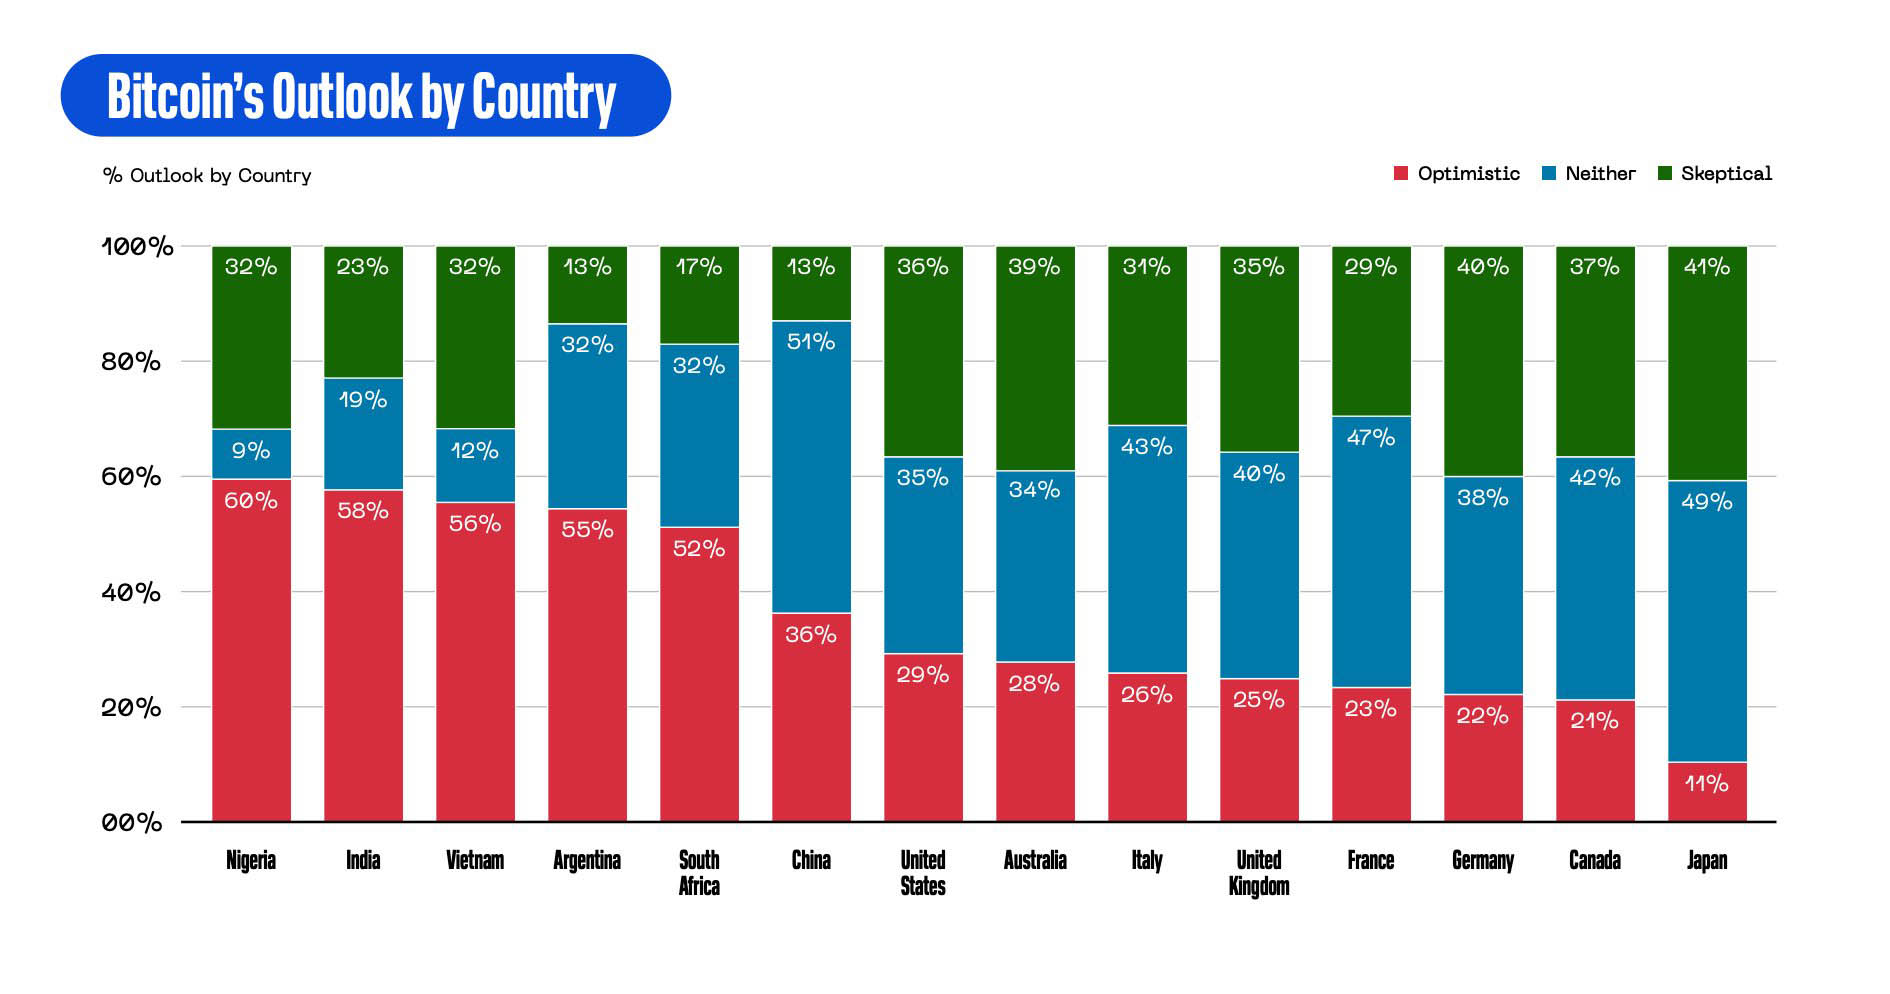
\includegraphics[width=\linewidth]{optimism}
	\caption{\href{https://twitter.com/gladstein/status/1532054253673406464}{``This new chart from Block is financial privilege visualized.''}}
	\label{fig:optimism}
\end{figure*}
Gladstein's is a carefully developed and well researched book, but is written from the perspective of (just) Bitcoin `being the raft'. Later in this book we will consider if it might be the iceberg, but this is not the domain expertise we offer in this book. \par
To further contextualise this \href{https://www.youtube.com/watch?v=BRQIMjZLMDk}{Mike Novogratz} claims the adoption figures at the top of the page. 
\href{https://dailyhodl.com/2022/05/04/crypto-winter-unlikely-as-astonishing-user-growth-dwarfs-internet-adoption-rate-macro-guru-raoul-pal/}{Raoul Pal of RealVision} says: \textit{Crypto adoption is now massively outperforming the internet. It’s been growing at about 165\% a year versus 85\% for the internet for the same period of time now.} \par
Thanks to a natural fit with strong encryption, and innate resistance to censorship by external parties, these systems do lend themselves well to `borderless' applications, and are somewhat resistant to global regulation (for good or ill). Given the rates of adoption seen above it seems that this stuff is coming regardless of their somewhat marginal usefulness. This provides us an excellent use case to explore for metaverse applications, and this will be the focus.
\input{03_adoption_table}
\section{A panoply of tech}
Within DLT/blockchain there seem to be as many opinions on the value of the technology as there are implementations. A host of well engineered open source code repositories makes the cost of adoption relatively low. \par%Unfortunately there are many more repositories that look very similar and essentially scams.\par
There are thousands of different `chains' and many more tokens which represent value on them. A majority of these are code forks of earlier projects. Most \href{https://99bitcoins.com/deadcoins/}{are defunct} yet still have some residual `value' locked up in them as a function of their `distributed' tokens. \par 
Because the space is comparatively new, subject to \href{https://www.esma.europa.eu/press-news/consultations/call-evidence-dlt-pilot-regime}{scant regulation}, and often open source, it is possible to clone a github, change a few lines of code, and front it with a website in order to create `scams', and this happens frequently \cite{golumbia2020cryptocurrency}.\par
The following sections give an overview of the major strands of the technology. First is Ethereum, mainly to discount it's use for our needs, and move on to more appealing options.
\section{Ethereum}
Ethereum \cite{buterin2013ethereum} is the second most \href{https://www.crypto51.app/}{secure} public blockchain (\href{https://howmanyconfs.com/}{by about 50\%})\cite{sayeed2019assessing}, and second most valuable by \href{https://coinmarketcap.com/}{market capitalisation} (though this comparison is somewhat stretched). It is the natural connection from Web3 to the rest of the book, so it will be considered first.\par
It is touted as `programmable money'. It, unlike bitcoin, is (\href{https://hackernoon.com/turing-completeness-and-the-ethereum-blockchain-c5a93b865c1a}{nearly}) Turing complete \cite{petzold2008annotated}, able to run a \href{https://ethereum.org/en/developers/docs/evm/}{virtual machine} within the distributed network (albeit slowly), and can therefore process complex transactional contracts in the settlement of value. This has given rise to the new field of `distributed finance', or DeFi (described later), alongside many interesting trust-minimised immutable ledger public database ideas. \par
There are trade-offs and problems with Ethereum (Eth/Ether) which currently increase the `participation floor' and make the network far less suitable for entry level business-to-business use. The ledger itself being a computational engine, with write only properties, is enormous. Specialist cloud hardware is required to run a full node (copy of the ledger), and partial nodes are the norm. Many partial nodes are run by one specialist cloud provider (\href{https://consensys.net/blog/news/why-infura-is-the-secret-weapon-of-ethereum-infrastructure/}{Infura}), which has recently been forced to \href{https://finance.yahoo.com/news/metamask-infura-block-certain-areas-173749914.html}{exclude Venezuela} from the network. A staggering 50\% runs on \href{https://ethernodes.org/networkType/Hosting}{Amazon AWS servers}. Critics of the project point to these vulnerabilities to outside influence as an existential threat to the aims of the technology. If it can be censured, then what advantage is there over the \href{https://protos.com/consensys-lawsuit-jpmorgan-owns-critical-ethereum-infrastructure/}{founders} simply running a high speed database to the same purpose? \par
This is a function of the so called `scalability trilema' \cite{hafid2020scaling}, in which it seems that only two features from the list of decentralization, scalability or security can be chosen for blockchains \cite{bonneau2015sok}.\par
Moreover the network is centrally controlled by its creator and the `miners'. There is a strong case to answer that Eth is \href{https://blog.mollywhite.net/blockchains-are-not-what-they-say/}{neither distributed}, nor trustless, and in fact therefore fails to be differentiated from a DLT, undermining some of it's claims. The history of Ethereum is a fascinating case study in human greed. By the time the whitepaper had it's first limited release, Bitcoin (covered next) had already passed \$1000 per token. This led to the creators ambitions for a `fair release' of tokens being voted down by powerful funders, leading to the explosion of similarly structured `pre-mined' coins in the ICO craze, which followed on the Ethereum network. Laura Shin is possibly the most experienced journalist and author in the space and has covered this crazy era in her book `The Cryptopians' \cite{cryptopians}. It's a tough read for the newcomer though, perhaps finish this primer first!\par
With that said there are many talented developers doing interesting work on the platform, and innovation is fast paced. It is entirely normal for technology projects to launch their distributed ledger idea on and within the Ethereum network. These generate tradable `ERC-20' tokens, which can accrue value or demonstrate smart contract utility  (based on the \href{https://soliditylang.org/}{Solidity} programming language). Because the value locked and generated in the Ethereum platform comes not just from the ETH token, but all the ERC technologies built upon it, there are hundreds of billions of pounds `within' the network. Most of this money is pure market speculation (as is the case across blockchains). Many analysts cannot see this as anything but a speculative bubble, with all the predictable crash yet to come. This can be seen in the context of other bubbles in Figure \ref{fig:etherbubble}. It seems that most of the projects in crypto more generally, but certainly with ETH and the NFTs within it are a new kind of social gambling, where online communities can reinforce groupthink around their speculative choices. With all this said most of the couple of million people who use NFTs use Ethereum, and if this market of creators and consumers is to be brought into a mixed reality space then they will need a way to bring their objects with them. 
\begin{figure}
  \centering
    \includegraphics[width=\linewidth]{etherbubble}
  \caption{Ethereum is thought to look like a speculative bubble. Rights requested}
    \label{fig:etherbubble}
\end{figure}

Such is the level of nefarious activity on these networks (within Ethereum) that they have a poor reputation, and are difficult to audit, launch, and maintain. The overriding problem of using a blockchain for utility applications (rather than just as money) is that people can, and will, simply lie for criminal purpose when entering data into the ledger. It is far more likely that Ethereum is simply a speculative bubble than any of the claims for utility being born out. Add to that \href{https://advisor.morganstanley.com/daron.edwards/documents/field/d/da/daron-edwards/Cryptocurrency_201__What_is_Ethereum_.pdf}{Morgan Stanleys recent assertion} that Ethereum is itself threatened by newer contender chains and it's future becomes unclear. The report correctly identifies that ``High transaction fees create scalability problems and threaten user demand. High costs make Ethereum too expensive for small-value transactions.''. It is this high cost of use that most excludes the ERC-20 networks from our consideration.
\subsection{Mining and Gas}
Ethereum has a significant barrier to entry because of high fees to use the network. The system is Turing complete; able to programatically replicate any other computational system. This includes endless loops in code, so it is trivial to lock up the computational bandwidth of the whole system, in a smart contract commitment, through a web wallet. \par 
To mitigate this existential `denial of service attack' the `gas' system demands that users spend some of their locked up value to operate on the network. In this way a transaction loop would quickly erode the available gas and stop looping. As the popularity of the system has grown, so too have the gas fees. It can \href{https://twitter.com/Blockworks_/status/1521071340517830657}{sometimes cost} over £10,000 to do a single transaction, though it is typically a few tens of pounds. Appallingly if the user pitches their mining fee offer too low, then the money gets spent anyway! \href{https://fees.wtf/#/}{A website} just plucks random Ethereum addresses out of the aether to show you the level of this expense for participants. People can even \href{https://opensea.io/collection/fees-wtf-nft?search[sortAscending]=false&search[sortBy]=PRICE}{buy NFTs} of the worst examples of these, as `tokens', wasting more money. This is a huge problem for potential uses of the network. \par
It is currently a proof of work system like Bitcoin (this is described in the next section), and has a \href{https://news.trust.org/packages/cryptocurrency-and-climate/}{commensurate energy footprint} to secure the network. It also ties up global \href{https://www.techradar.com/in/news/ethereum-miners-spent-dollar15-billion-on-gpus-in-just-over-one-year}{supply of PC graphics cards} used for it's mining model, making them far more expensive. This has generated ill will in the global gamer community for instance, and damped the ambitions of NFT developers because of their inability to sway this crucial customer demographic. Much more on this later.\par
\subsection{Upgrade roadmap}
Part of the challenge Ethereum faces is wrapped up with it's complex token emission schedule. This is the rate at which tokens are generated and `burnt' or destroyed in the network. The total supply of tokens is uncertain, and both emission and burn schedules are regularly tinkered with by the project. The changes to the rate at which ETH are generated can be seen in Figure \ref{fig:ethemission}.
\begin{figure}
  \centering
    \includegraphics[width=\linewidth]{ethemission}
  \caption{The rate of token generation has changed unpredictably over time. Rights requested}
  \label{fig:ethemission}
\end{figure}
In addition, a recent upgrade (EIP-1559) results in tokens now being burnt at a higher rate than they are produced, deliberately leading to a diminishing supply. In theory this increases the value of each ETH on the network at around 3\% per year. It's very complex, with impacts on transaction Fees, waiting time, and consensus security, as examined by Liu at al. \cite{liu2022empirical}. Addionally, there is now talk (by \href{https://time.com/6158182/vitalik-buterin-ethereum-profile/}{Butlerin}, the creator of Ethereum) of extending this burn mechanism \href{https://ethresear.ch/t/multidimensional-eip-1559/11651}{further into the network}.\par
Ethereum was designed from the beginning to move to a `proof of stake' model where token holders underpin network consensus through complex automated voting systems based upon their token holding. This is now called \href{https://blog.ethereum.org/2022/01/24/the-great-eth2-renaming/}{Ethereum Consensus Layer}. Proof of stake has problems in that the majority owners `decide' the truth of the chain to a degree, and must by design have the ability to over-ride prior consensus choices. Proof of stake is probably inherently broken \cite{poelstra2015stake}. This has \href{https://notes.ethereum.org/@djrtwo/risks-of-lsd} for malicious actors who have sufficient control of the existing history of the chain, \href{https://twitter.com/MTorgin/status/1521433474820890624}{thought to be} in the region of \$50M \cite{mackinga2022twap}. Like much of the rest of `crypto' the proposed changes will concentrate decisions and economic rewards in the hands of major players, early investors, and incumbents. This is a far cry from the stated aims of the technology. The move to proof of stake has recently earned it the \href{https://www.technologyreview.com/2022/02/23/1044960/proof-of-stake-cryptocurrency/}{MIT breakthrough technology award}, despite not being complete. It's clearly a technology which is designed to innovate at the expense of predictability. This might work out very well for the platform, but right now the barrier to participation (in gas fees) is so high that we do not intend for Ethereum to be in scope as a method for value transfer within metaverses.\par


\section{Bitcoin}
The first blockchain was the Bitcoin network \cite{Nakamoto2008}, some two decades after Haber et al. first described the idea \cite{haber1990time}. Prior to Bitcoin these structures were called `timechains' \cite{nakamoto2018}. It can be considered a triple entry book keeping system \cite{ijiri1986framework, faccia2019accounting}, the first of it's kind, integrating a `provable' timestamp with a transaction ledger, solving the ``double spend problem'' \cite{chohan2021double, perez2019double, grunspan2018double}. Some see this as the first major innovation in ledger technology since double entry was codified in Venice in fourteen seventy five\cite{sangster2015earliest}. \par
It was created pseudonomously by an individual or group calling themselves `Satoshi Nakamoto' in 2009, as a direct response to the perceived mishandling of the 2008 global financial crisis \cite{nakamoto2018}, with the stated aim of challenging the status quo, with an \href{https://world.hey.com/dhh/i-was-wrong-we-need-crypto-587ccb03}{uncensorable} technology, to create a money which could not be \href{http://p2pfoundation.ning.com/forum/topics/bitcoin-open-source}{debased by inflation policy}, and outside of the \href{https://www.coindesk.com/layer2/2022/05/04/matt-taibbi-paypals-deplatforming-and-the-case-for-crypto/}{politically captured} fintech incumbents. It's interesting to note that the narrative around the use case for Bitcoin has \href{https://uncommoncore.co/visions-of-bitcoin-how-major-bitcoin-narratives-changed-over-time/}{shifted over it's lifetime}. \par
The \href{https://en.bitcoin.it/wiki/Genesis_block}{``genesis block''} which was hard coded at the beginning of the `chain' contains text from The Times newpaper detailing the second bank bailout.\par 
There will only ever be (\href{https://blog.amberdata.io/why-the-bitcoin-supply-will-never-reach-21-million}{just short of}) 21 million bitcoins issued, of which around 19 million have already been minted, and around 4 million lost forever. This `hard money' absolute scarcity is a strong component of the Bitcoin meme landscape. These are basically arbitrary figures though; a combination of the issuance schedule, and an \href{https://plan99.net/~mike/satoshi-emails/thread1.html}{`educated guess'} by Nakamoto: \cite{nakamoto2018}\par 
\textit{''My choice for the number of coins and distribution schedule was an educated guess.  It was a difficult choice, because once the network is going it's locked in and we're stuck with it.  I wanted to pick something that would make prices similar to existing currencies, but without knowing the future, that's very hard.  I ended up picking something in the middle.  If Bitcoin remains a small niche, it'll be worth less per unit than existing currencies.  If you imagine it being used for some fraction of world commerce, then there's only going to be 21 million coins for the whole world, so it would be worth much more per unit.''}\par
In theory there is no \href{https://www.forbes.com/sites/peterizzo/2021/09/29/against-cryptocurrency-the-ethical-argument-for-bitcoin-maximalism/?}{barrier to access}, and \href{https://www.coindesk.com/layer2/2022/02/16/why-bitcoin-is-a-tool-for-social-justice/}{equality of opportunity} to accumulate and save over long periods. This is not true of chains and tokens since, which lock up some of their value for seed investors to cash out later. None of the blockchains since are decentralised in the same way \cite{selvam2021blockchain}. Bitcoin was probably a \href{https://danhedl.medium.com/bitcoins-distribution-was-fair-e2ef7bbbc892}{singular event}.\par
Each Bitcoin can be divided into 100 million satoshis (sats), so anyone buying into Bitcoin can buy a thousandth of a pound, assuming they can find someone willing to transact that with them. \par
Satoshi Nakamoto (the name of the publishing entity) \href{https://bitcoinmagazine.com/technical/what-happened-when-bitcoin-creator-satoshi-nakamoto-disappeared}{disappeared from the forums} forever in 2010. Bitcoin has the marks of cypherpunks and anarcho capitalism. The IMF has recently conceded that the Bitcoin \href{https://blogs.imf.org/2022/01/11/crypto-prices-move-more-in-sync-with-stocks-posing-new-risks/}{poses a risk} to the traditional financial systems, so it could be argued that it is succeeding in this original aim.\par
Although there were some earlier experiments (hashcash, b-money etc), Bitcoin is the first viably decentralised `cryptocurrency'; the network is used to \href{https://www.aier.org/article/why-does-bitcoin-have-value/}{store economic value} because it is judged to be secure and trusted. It is a singular event in that it became established at scale, such that it could be seen to be a fully distributed system, without a controlling entity. This is the differentiated trust model previously mentioned. This relative security is the specific unique selling point of the network. It is many times more secure than all the networks which came after based on a like for like comparison of \href{https://howmanyconfs.com/}{transaction `confirmations'}. This network effect of Bitcoin is a compounding feature, attracting value through the security of the system. It is deliberately more conservative and feature poor, preferring instead to \href{https://bips.xyz/}{add to it's feature set} slowly, preserving the integrity of the value invested in it over the last decade. At time of writing it is a \href{https://fiatmarketcap.com/}{top quartile} largest global currency and has settled over \$13 trillion Dollars in 2021, though Makarov et al. contest this, citing network overheads, and speculation \cite{makarov2021blockchain}. Institution grade `exchange tradable funds' which allow investment in Bitcoin are available throughout the world, and the native asset can be bought by the public easily through apps in all but a handful of countries as seen in Figure \ref{fig:settled2021}. \par
\begin{figure}
  \centering
    \includegraphics[width=\linewidth]{settlement2021}
  \caption{\href{https://twitter.com/glxyresearch/status/1469039427028664320?}{Growth in settlement} value on the Bitcoin network (Forbes).}
  \label{fig:settled2021}
\end{figure}
Only around 7 transactions per second can be settled on Bitcoin. The native protocol does not scale well, and this is an inherent trade-off as described by Croman et al. in their positioning paper on public blockchains \cite{croman2016scaling}. Over time, competition for the limited transaction bandwidth drives up the price to use the network. This effectively prices out small transactions, even locking up some value below what is a termed the '\href{https://github.com/bitcoin/bitcoin/blob/v0.10.0rc3/src/primitives/transaction.h#L137}{dust limit}' of unspent transactions too small to ever move again \cite{delgado2018analysis}. \par
Bitcoin has developed quickly, with a \href{https://phemex.com/blogs/crypto-bitcoin-s-curve-adoption-curve}{faster adoption} than even the internet itself. It is already a mature ecosystem, and is seeing adoption as a \href{https://bitcointreasuries.net/}{corporate treasury asset}. \par
Adoption by civil authorities is increasing, and legislators the world over are being forced to \href{https://www.politico.com/news/2022/01/16/bitcoin-crashes-the-midterms-527126}{adopt a position}. California has an \href{https://www.gov.ca.gov/2022/05/04/governor-newsom-signs-blockchain-executive-order-to-spur-responsible-web3-innovation-grow-jobs-and-protect-consumers/}{explicitly Web 3 and blockchain executive order} to invetigate and support opportunities. Many city treasuries have \href{https://www.bloomberg.com/news/articles/2022-01-14/rio-de-janeiro-wants-to-become-brazil-s-cryptocurrency-capital}{added it} to their balance sheet. The Swiss city of Lugano is launching a \href{https://twitter.com/Stadicus3000/status/1499656424422526977}{huge initiative} alongside Tether. It is already legal tender in the country of El Salvador\cite{oxford2021salvador} and the \href{https://finance.yahoo.com/news/central-african-republic-passes-bill-180910797.html?}{Central African Republic}, and will be soon in \href{https://www.forbes.com/sites/ninabambysheva/2022/04/07/two-new-territories-are-adopting-bitcoin/?sh=7f014ed2499a}{Madeira and Roatán island}. This means it \textit{must} be accepted as a means of payment. In places such as Panama it simply has legal status and \textit{can} be accepted without double taxation.\par 
Global asset manager ``Fidelity'' wrote the following in their \href{https://www.fidelitydigitalassets.com/articles/2021-trends-impact}{2021 trends report}. \textit{``We also think there is very high stakes game theory at play here, whereby if Bitcoin adoption increases, the countries that secure some bitcoin today will be better off competitively than their peers. Therefore, even if other countries do not believe in the investment thesis or adoption of bitcoin, they will be forced to acquire some as a form of insurance. In other words, a small cost can be paid today as a hedge compared to a potentially much larger cost years in the future. We therefore wouldn't be surprised to see other sovereign nation states acquire bitcoin in 2022 and perhaps even see a central bank make an acquisition.''}\par
\subsection{The Bitcoin Network Software}
There isn't a single GitHub which can be considered the final arbiter of the development direction, because it is a distributed community effort with some \href{https://decrypt.co/66740/who-are-the-fastest-growing-developer-communities-in-crypto}{500 developers} out of a wider `crypto' pool of around 9000 contributors (the vast majority are spread across disparate Ethereum and some Solana projects). \href{https://bitcoinops.org/en/newsletters/2021/12/22/}{Development and innovation continues} but there is an emphasis on careful iteration to avoid damage to the network. Visualisation of code commitments to the various open source software repositories can be seen at \href{https://www.youtube.com/channel/UC4DT4qudqogkmbqVAQy8eFg/videos}{Bitpaint youtube channel} and in Figure \ref{fig:gource}.\par
\begin{figure*}[ht]\centering % Using \begin{figure*} makes the figure take up the entire width of the page
	\includegraphics[width=\linewidth]{gource}
	\caption{\href{https://github.com/bitpaint/bitcoin-gources}{Bitpaint}: Contributions to the Bitcoin ecosystem. Reused with permission.}
	\label{fig:gource}
\end{figure*}
\href{https://github.com/bitcoin/}{Bitcoin core} is the main historical effort, but there are alternatives (\href{https://github.com/libbitcoin/libbitcoin-node/wiki}{LibBitcoin in C++}, \href{https://github.com/btcsuite/btcd}{BTCD in Go}, and \href{https://bitcoinj.github.io/getting-started}{BitcoinJ in Java}), and as innovation on layer one slows, attention is shifting to codebases which interact with the base layer asset. Much more on these later.
\subsection{Mining and Energy concerns}
\subsubsection{Mining process overview}
Bitcoin mining is the process of adding public transactions into the ledger, in return for two economic rewards, paid in Bitcoin. These are the mining fee, and the block reward. The transactions which are added into the next `block' of the chain are selected preferentially based on the fee they offer, which is up to the user trying to get their transaction into the chain. This can be within the next 10 minutes (next block), or a gamble out toward 'never' depending how competitive the network is at any time. Miners try to find a sufficiently low result from a cryptographic hash function \cite{rogaway2004cryptographic}(a random process), and upon finding it, they can take their pre-prepared `block' of transactions sourced from their local queue (mempool), and add it into the chain, for confirmation by other miners. In return they take all the fees within that mined block, and whatever the block reward is at the time. When the network started the block reward was 50 Bitcoin, but has \href{https://ma.ttias.be/dissecting-code-bitcoin-halving/}{halved} repeatedly every 210,000 blocks (four years) and now stands at 6.25 BTC. The rate of mining is kept roughly at one block every 10 minutes, by a difficulty adjustment every 2016 blocks (2 weeks). This in a complex interdependent mechanism and is explained very well in \href{https://bitcoinmagazine.com/technical/how-mining-protects-the-bitcoin-network}{this article}. These components are explained in slightly more detail later.\par
\subsubsection{Energy use}
Bitcoin uses a staggering amount of energy to secure the blockchain, and this \href{https://www.edmundconway.com/bitcoin-money-and-the-planet/}{has climate repercussions}. A simple back of the envelope use of the \href{https://www.iea.org/reports/key-world-energy-statistics-2021/supply}{IEA total energy supply}, and the \href{https://ccaf.io/cbeci/index}{Cambridge Bitcoin energy use} estimate puts the network at \href{https://www.wolframalpha.com/input?i=153+terawatt+hours+as+percentage+of+\%28600+exa+joules+as+terrawatt+hours\%29+}{around 0.1\%} of global energy use.\par
It is an \href{https://www.ruetir.com/2022/03/18/riot-whinstone-the-bitcoin-farm-with-100000-computers-that-uses-excess-energy-from-an-oil-platform-to-mine-cryptocurrencies-ruetir/}{industrial scale} global business with `mining companies' investing \href{https://ir.marathondh.com/news-events/press-releases/detail/1272/marathon-digital-holdings-bitcoin-mining-fleet-to-reach}{hundreds of millions of pounds} at a time in specialist \href{https://en.wikipedia.org/wiki/Application-specific_integrated_circuit}{ASIC} mining hardware and facilities. The latest purpose designed Intel chip \href{https://www.intel.com/content/www/us/en/newsroom/opinion/thoughts-blockchain-custom-compute-group.html#gs.pd9ofu}{touts} both Web3 and metaverse applications. This is ``proof of work'',  and is essential to the technology, and is still thought to be the \href{https://www.truthcoin.info/blog/pow-cheapest/}{best available option}. \href{https://ccaf.io/cbeci/index}{The Cambridge Bitcoin Energy Consumption Index} monitors this energy usage. Their \href{https://www.jbs.cam.ac.uk/insight/2022/bitcoin-mining-new-data-reveal-a-surprising-resurgence/}{2022 report} sees American mining leading globally.\par
Such businesses can mine a Bitcoin for \href{https://www.911metallurgist.com/blog/the-cost-to-mine-different-cryptocurrencies-in-every-country}{around \$5k-\$10k} per coin, so the profit margins \href{https://www.nicehash.com/profitability-calculator}{are considerable} (based on 30-40 Joule/terahash and power rate less than 5 cents/kilowatt hour and excluding hardware costs). This is not to say that all mining is, or should be, so concentrated. Anyone running the hashing algorithm can \href{https://twitter.com/ckpooldev/status/1485585814419812356}{get lucky} and claim the block reward. PoW ties the value of the `money' component of Bitcoin directly to energy production. This is not a new idea. Henry Ford proposed an intimate tie between energy and money to create a separation of powers from government, as can be seen in Figure \ref{fig:energyNYT}.\
\begin{figure}
  \centering
    \includegraphics[width=\linewidth]{energyNYT}
  \caption{\href{https://www.nytimes.com/1921/12/06/archives/mr-fords-energy-dollar.html}{Intimate tie between energy and money, Henry Ford}}
  \label{fig:energyNYT}
\end{figure}
The potential ecological footprint of the network has always been a concern; Hal Finney himself was \href{https://twitter.com/halfin/status/1153096538}{thinking about this issue} with a mature Bitcoin network as early as 2009, and \href{https://satoshi.nakamotoinstitute.org/posts/bitcointalk/threads/167/#35}{a debate} on the Bitcoin mailing lists called the mining process ``thermodynamically perverse'' \par
\href{https://electricmoney.org/}{Proponents of the technology} say that the balance shifted dramatically in 2021 with China outright banning the technology; this has forced the bulk of the energy use \href{https://docs.google.com/spreadsheets/d/1E7489rM7Q62oXwk1f4NUlMvok9noAbpYfTynY2VTyww/edit#gid=0}{toward the USA}, and away from `dirty coal' as seen in Figure \ref{fig:miningshare}. Some analysts \href{https://docs.google.com/document/d/1N2N-5jY00cmteoY_puWI9oosM1foa4EQqsO1FFfIFR4/edit}{have proposes mitigations} \cite{cross2021greening}. As a worked example of \href{https://docs.google.com/spreadsheets/d/15e_a-D3x4fv3tglEzFmQ6TLQx0fZe6-iKO9Fc9SyISQ/edit#gid=0}{Cross and Bailey's proposal} a retail investor owning 1 BTC would have to buy around 700 shares of `CleanSpark' mining company (CLSK) to make their \href{https://docs.google.com/spreadsheets/d/1r32T8p_PHTP8S781u7PhPSwehLx2VcJTaJJKesMswD0/edit#gid=0}{holding completely neutral}.  Some more strident voices suggest that \href{https://medium.com/@magusperivallon/a-financial-hail-mary-for-the-climate-an-argument-for-bitcoin-adoption-9c58e707d0}{`ending financialisation' through use of Bitcoin} may be net positive for the environment at a macro level \cite{bitcoinisvenice}. Indeed it may \href{https://www.newsweek.com/bitcoin-mining-americas-most-misunderstood-industry-opinion-1669892}{provide a route} to support \href{https://mobile.twitter.com/DSBatten/status/1514072998881665027}{electrifying everything} through deployment of \href{https://lancium.com/solutions/}{flexible base load}, and local subsidy initiatives (as may be \href{https://braiins.com/blog/bitcoin-mining-the-grid-generators}{happening in Texas})\cite{griffith2021electrify, ercotimpact2021}. Brad Jones, \href{https://www.youtube.com/watch?v=gKnRfDeFgr0}{interim CEO of the Texas grid said}:\par
\textit{``As we get more renewable generation, in particular wind [which] is operating at night ...  we have to find a home for it, otherwise we have to turn the wind down. It’s such a great resource we shouldn’t turn it down. Bitcoin mining or what some call crypto has found a way to come into our markets and take some of that wind in off-peak periods. Then when we get to peak period times they are very quick to remove themselves from the market as prices increasesThe.  fact that we can turn down whenever we need the power for other customers is fantastic. We can use that crypto currency to soak up that excess generation when there’s a lot of that, and find a home for more solar and more wind to come to our grid. Then they reduce consumption when we need that power for other customers. So it’s a great balancing act. Most other datacenters [such as] Microsoft or Amazon have other customers to serve every other day, so they can’t just turn off. But these crypto customers can. If the cost of energy gets too high they can remove themselves from the market. They are also helpful if we lose a generator. They can quickly respond to that frequency disruption and allow us to balance our grid.''}\\
This \href{https://www.citadel21.com/bitcoin-is-the-first-global-market-for-electricity-and-will-unleash-renewables}{``global energy market''} revolution is explained by Tabatabai of Modo Energy.\par Recently for example Baur and Oll found that \textit{``Bitcoin investments can be less carbon intensive than standard equity investments and thus reduce the total carbon footprint of a portfolio.''}\cite{baur2021bitcoin}. Perhaps of note for the near future is that KPMG whose investment was mentioned in the introduction also matched their position in the space with equivalent  carbon offsets. This may provide an investment and growth model for others.
\begin{figure}
  \centering
    \includegraphics[width=\linewidth]{miningshare}
  \caption{Hash rate \href{https://ccaf.io/cbeci/ining_map}{suddenly migrates} from China [Reuse rights requested]}
  \label{fig:miningshare}
\end{figure}
The power commitment to the network is variously projected \href{https://www.nature.com/articles/s41558-018-0321-8}{to increase}, or \href{https://assets.website-files.com/614e11526f6630959fc98679/616df63a27a7ec339f5e6a80_NYDIG-BitcoinNetZero_SML.pdf}{level off over time}, but certainly not decrease. The \href{https://www.forbes.com/sites/martinrivers/2022/04/03/is-bitcoin-really-that-bad-for-the-environment/?sh=6a3203427143}{industry now argues} that economic pressures mean that most of the `hashrate' is \href{https://bitcoinminingcouncil.com/q4-bitcoin-mining-council-survey-confirms-sustainable-power-mix-and-technological-efficiency/}{generated by renewable energy}\cite{blandin20203rd}. As a recent example of this trend Telsa (Elon Musk), Block (Twitters Jack Dorsey), and Blockstream (Adam Back) are teaming up to \href{https://www.cnbc.com/2022/04/08/tesla-block-blockstream-to-mine-bitcoin-off-solar-power-in-texas.html}{mine with solar energy} in Texas.\par 
There is growing interest and adoption of so called \href{https://www.bloomberg.com/news/articles/2022-06-01/oman-backs-u-s-firm-mining-crypto-to-cut-natural-gas-flaring}{``stranded energy mining''}  which cannot be effectively transmitted to consumers, and is thereby sold at a huge discount while also \href{https://www.renewableenergyworld.com/wind-power/900mw-wind-farm-to-power-bitcoin-mining-operation/}{developing power capacity}, without the \href{https://batcoinz.com/the-renewable-energy-cannot-happen-without-bitcoin-mining\%ef\%bf\%bc/}{usual constraints} \cite{bastian2021hedging}, \href{https://www.curbed.com/2021/07/crypto-currency-mining-old-power-plants.html}{re-purposing historic} infrastructure, and/or \href{https://www.bloomberg.com/news/articles/2022-03-24/exxon-considers-taking-gas-to-bitcoin-pilot-to-four-countries}{reducing the carbon} (or \href{https://batcoinz.com/quantifying-the-potential-impact-of-bitcoin-mining-on-global-methane-emissions-4/}{more interestingly} the methane) of existing infrastructure. Adam Wright of \href{https://vespene.energy/}{Vespene Energy} says: \textit{``You could either mine Bitcoin on one small landfill for a year, or you could plant 5 million trees and let them grow for 10 years - both of those are going to have the same environmental impact.''}\par
Cheikosman, a policy analyst for the World Economic Forum (somewhat surprisingly) \href{https://www.weforum.org/agenda/2022/03/crypto-energy-consumption/?}{wrote} \textit{``Crypto is becoming an essential part of developing a carbon-neutral energy grid and has made it economically viable to invest in, develop and build renewable energy power generation.''} 
The market economics of this are far from simple, but are well explained by \href{https://www.whatbitcoindid.com/podcast/bitcoin-energy-markets}{Connell in a podcast}. 
The most cited example of building capacity before grid connection is El Salvador's `volcano mining' proposal, which is supporting their national power infrastructure plans. Uzbekistan seems to be promoting a \href{https://www.reuters.com/business/finance/uzbekistan-legalises-solar-powered-crypto-mining-2022-05-04/}{similar model} with zero tax provided the Bitcoin mining companies build out their own solar infrastructure. A more poignant example is the \href{https://www.timesunion.com/news/article/Mechanicville-hydro-plant-gets-new-life-16299115.php}{Mechanicville hydro plant in the USA}. The refurbishment of this 123 year old power plant is being funded by Bitcoin mining. This is the \href{https://www.lynalden.com/bitcoin-energy/}{``buyer of last resort''} model first \href{https://squareup.com/us/en/press/bcei-white-paper}{advanced by Square Inc}.\par
Conversely it might be that vertical integration of Bitcoin mining \href{https://bitcoinmagazine.com/business/oil-companies-partner-with-bitcoin-miners}{within legacy fossil fuel stations} gives them a new lease of life.\par%A \href{https://twitter.com/thelaserlife/status/1511354396705452035}{pseudonymous twitter user} puts this well:\par 
%\textit{``Eventually it'll seem obvious – having a mechanism to instantly monetize energy at its source was the missing ingredient to massively scale up green energy production.''}. Critics highlight the potential \href{https://www.fitchratings.com/research/us-public-finance/crypto-mining-poses-challenges-to-public-power-utilities-24-01-2022}{impact of mining on local energy} prices\cite{benetton2021cryptomining}.\par
\href{https://www.youtube.com/watch?v=6LP8G-oZnEs}{The debate} whether this consumption is `worth' it is \href{https://www.utilitydive.com/news/bitcoin-mining-as-a-grid-resource-its-complicated/617896/}{complex} and \href{https://www.aei.org/technology-and-innovation/no-hearing-on-bitcoins-energy-use-is-complete-without-nic-carter/}{rapidly evolving}. Useful examples of this are:
\begin{itemize}
\item the \href{https://www.zerohedge.com/crypto/questionable-ethics-anti-bitcoin-esg-junk-science}{online pushback} to an academic article by PhD candidate de Vries et al, which was based on an undergraduate class discussion and has had an outsized effect on global policy \cite{de2022revisiting}, 
\item a \href{https://rebrand.ly/v8qq1sx}{paper from the Bitcoin Policy Institute}, 
\item and the industry \href{https://bitcoinminingcouncil.com/wp-content/uploads/2022/05/Bitcoin_Letter_to_the_Environmental_Protection_Agency.pdf}{open letter to the EPA}.\par
\item this well considered \href{https://twitter.com/jyn_urso/status/1508899761319038983}{Twitter thread} by climate scientist Margot Paez.
\end{itemize}
This stuff is existentially important to the whole technology. Is a trillion dollar asset which \href{https://www.theheldreport.com/p/bitcoin-vs-gold}{potentially replaces} the money utility of gold, but doesn't need to be stored under guard in vaults (Figure \ref{fig:goldmanVgold}), worth the equivalent power consumption of clothes dryers in North America? Probably not with the current level of adoption, but this is an experiment in replacing global money. If that were to happen then Bitcoin would be around 50 times more efficient than the current system according to Khazzaka \cite{khazzaka2022bitcoin}. To be clear it's not the position of this book that replacing Fiat money is a good idea, but the experiment is being run regardless. This is explored in it's own chapter later.\par
It seems possible that three value propositions are therefore emerging:
\begin{itemize}
\item Bitcoin the speculative asset (or greater fool bubble \cite{de1990positive}). Nations such as the USA, who own 30\% of the asset have bid up the price of the tokens during a period of very cheap money, and this has led to a high valuation for the tokens, with a commensurately high network security through the hash rate (mining). This could be a speculative bubble, with the asset shifting to one of the other valuations below.
\item Bitcoin the monetary network, and `emerging market' value transfer mechanism. There is no sense of the ``value'' of this network at this time, but it's the aspect we need for our metaverse application. For this use the price must simply be high enough to ensure that mining viably secures the network. This security floor is unfortunately a `known unknown'. If a global Bitcoin monetary axis evolves (as in the Money chapter later) the network would certainly require a higher rate than currently, suggestive of a higher price of token to ensure mining.
\item Bitcoin as a flexible load in power distribution systems. Again there is no price against this, but we can perhaps grossly estimate it at around half the current hash rate if 50\% of the network is currently green energy. This would imply a price for the asset roughly where it is now (ie, not orders of magnitude higher or lower).  
\end{itemize}
\begin{figure}
  \centering
    \includegraphics[width=\linewidth]{goldmanvgold}
  \caption{Goldman suggest growth opportunity and potential demonetisation of gold?}
  \label{fig:goldmanVgold}
\end{figure}
Legislators globally, are starting to codify their positions on proof of work as a technology (including Bitcoin). The USA is variously supporting or constricting the technology, according to \href{https://www.ncsl.org/research/financial-services-and-commerce/cryptocurrency-2021-legislation.aspx}{state legislatures}. Notably New York has \href{https://www.nysenate.gov/legislation/bills/2021/A7389}{banned new carbon intensive} mining facilities for 2 years, while rust and farm belt states with energy build-out problems are \href{https://financialpost.com/fp-finance/cryptocurrency/texas-governor-abbott-turns-to-bitcoin-miners-to-bolster-the-grid-and-his-re-election}{providing incentives}. \par
The EU has just voted to add the whole of `crypto', including PoW, to the EU taxonomy for sustainable activities. This EU wide classification system provides investors with guidance as to the sustainability of a given technology, and can have a meaningful impact on the flows of investment. With that said the report and addition of PoW is not slated until 2025, and it is by no means clear what the analysis will be by that point. Meanwhile they're tightening controls of transactions, on which there will be more detail later.  \par
We have seen that China has cracked down hard on the technology, banning mining and pressuring holders of the assets. They have unwound this somewhat, and based on past experience it seems that they will continue to nuance their position as they seek adoption of their own digital currency.\par
In India (a seemingly natural environment for crypto given the popularity of gold) there has been confusion for years as more ``local'' law vies with confusing central government signalling. It has variously been banned and unbanned, and is now subject to punitive tax. Ajay Seth, secretary of the Finance Ministry's Department of Economic Affairs recently said \textit{``We have gone through a deep dive consulting with not just the domestic and institutional stakeholders but also organizations like IMF and World Bank.... Simultaneously we are also beginning our work for some sort of a global regulation (to determine) what role India can play... Whatever we do, even if we go to the extreme form, the countries that have chosen to prohibit, they can't succeed unless there is a global consensus''}
\subsection{Technical overview}
This section could be far more detailed, but this is pretty complex stuff. Instead, there's plenty of \href{https://github.com/bitcoinbook/bitcoinbook}{books and websites} that do a more thorough job, if the reader is interested. Each subsection will include a good external link where more depth can be found. This whistle stop tour of the main components of the protocol should provide enough grounding, but it's not essential reading for non technical readers.\par
\subsubsection{ECDSA / SHA256 / secp256k1}
These technologies tend to use the same underpinning \href{https://curves.ulfheim.net/}{elliptic curve cryptography}, and it makes sense to unpack this here just once, only in the context of Bitcoin, as this will be the main focus of our attention.\par
In Bitcoin the ECDSA algorithm is used on the \href{https://en.bitcoin.it/wiki/Secp256k1}{secp256k1} elliptic function to create a trapdoor. This (essentially) one way mathematical operation was originally the ``discrete log problem'' and part of the research in cryptography by Diffie and Hellman \cite{diffie1976new}. This is what binds the public and private keys in a key pair. In their mathematical construct a modulus operator creates an infinite number of possible variations on operations which multiply enormous exponential numbers together, in different orders, to create key pairs. In order to reverse back through the `trapdoor' a probably impossible number of guesses would have to be applied.\par
Latterly, elliptic curves such as the secp256k1 curve used in Bitcoin have substantially simplified the computation problems. Rather than exponentials used by Diffie Helmman instead a repeated operation is applied to an elliptic curve function, and this itself creates a discrete log problem trapdoor in maths, far more efficiently. Figure \ref{fig:ECDSA} suggests how this works. \par
This makes it easier, faster, and cheaper to provide secure key pairs on basic computational resources. Elliptic curve solutions are not `provably' secure in the same way as the Diffie-Hellman approach, and the security of this system is very sensitive to the randomness which is applied to the operation. Aficionados of Bitcoin use dice rolls or \href{https://www.hackster.io/news/alex-waltz-s-quantum-random-number-generator-for-bitcoin-uses-radioactive-decay-and-a-raspberry-pi-25a75316220f}{even more exotic} means to add entropy (randomness) when creating keys. This really isn't necessary, the software does this well enough.\par  
ECDSA has already been replaced by the more efficient Schnorr signature method \cite{schnorr1989efficient}, but this will take some time for organic adoption, and ECDSA will never be deprecated.\par
\begin{figure}
  \centering
    \includegraphics[width=\linewidth]{ECDSA}
  \caption{Given a start point on the curve and a number of reflection operations it's trivial to find a number at the end point, but impossible to find the number of \href{https://github.com/bitcoinbook/bitcoinbook/blob/develop/ch04.asciidoc}{hops} from the two end points alone. (CC Mastering Bitcoin second edition)}
  \label{fig:ECDSA}
\end{figure}
\subsubsection{Bitcoin script}
A Bitcoin script is a short chunk of code written into each transaction which gives conditions for the next spend. The \href{https://bitcoin.sipa.be/miniscript/}{limited scripting language} and the features built into wallets on top, allow for some clever additional options beside receiving and spending. In fact, some of the more innovative features such as discrete log contracts (detailed later) are quite powerful, and can interact with the outside world. Scripts allow spends to be contingent on multiple sets of authorising keys, time locks into the future, or both.\par
\subsubsection{Addresses \& UTXOs}
Ethereum has addresses which transactions flow in and out of. This is synonymous to a bank account number and so makes intuitive sense to users of banks. This is not the case in Bitcoin.\par
Bitcoin is a UTXO model blockchain. UTXO stands for unspent transaction output, and these are `portions' of Bitcoin created and destroyed as value changes hands (through the action of cryptographic keys). They are the basis of the evolving ledger. This process is described well by Rajarshi Maitra in \href{https://medium.com/bitbees/what-the-heck-is-utxo-ca68f2651819}{this post}.\par
\textit{``Every Transaction input consists of a pointer and an unlocking key. The pointer points back to a previous transaction output. And the key is used to unlock the previous output it points to. Every time an output is successfully unlocked by an input, it is marked inside the blockchain database as `spent'. Thus you can think of a transaction as an abstract “action” that defines unlocking some previous outputs, and creating new outputs.\\
These new outputs can again be referred by a new transaction input. A UTXO or `Unspent Transaction Output' is simply all those outputs, which are yet to be unlocked by an input.\\
Once an output is unlocked, imagine they are removed from circulating supply and new outputs take their place. Thus the sum of the value of unlocked outputs will be always equal to the sum of values of newly created outputs (ignoring transaction fees for now) and the total circulating supply of bitcoins remains constant.''}\par
Fresh UTXOs are created as coinbase transactions, rewarded to miners who successfully mine a block. These can be spent to multiple output as normal. This is how the supply increases over time.
\subsubsection{Halving}
As mentioned eariler, roughly every four year the `block reward' given to miners halves. This gives the issuances schedule of Bitcoin; \href{http://bashco.github.io/Bitcoin_Monetary_Inflation/}{it's monetary inflation}. This `controlled supply' feature was added to emulate the growth of physical asset stocks through mining. It's exhaustively \href{https://en.bitcoin.it/wiki/Controlled_supply}{explained elsewhere} and is somewhat immaterial to our transactional use case in metaverse applications.
\subsubsection{Difficulty adjustment}
The difficult adjustment (also mentioned earlier) shifts the difficulty of the mining algorithm globally to re-target one new block every 10 minutes. This means that adding a glut of new mining equipment will increase the issuance of Bitcoins, in favour of the new mining entity, for up to 2 weeks, at which point the difficulty increases, the schedule resets, and the advantage to the new miner is diffused. Equally this protects the network against significant loss of global mining hashrate, as happened when China comprehensively banned mining. Again, this is explained in \href{https://en.bitcoin.it/wiki/Difficulty}{more detail} elsewhere.
\subsubsection{Bitcoin nodes }
The Bitcoin network can be considered a triumvirate of economic actors, each with different incentives. These are:
\begin{itemize}
\item Holders and users of the tokens, including exchanges and market makers, who make money speculating, \href{https://en.wikipedia.org/wiki/Arbitrage}{arbitraging}, and providing liquidity into the network. Increasingly this is also real `money' users of BTC, earning and spending in pools of circular economic activity. Perversely Bitcoin as a money is the fringe use case at this time.
\item Miners, who profit from creation of new UTXOs, and receive payments for adding transactions to the chain. In return they secure the network by validating the other miners blocks according the rules enforced by the node operators.
\item Node operators, \href{https://www.truthcoin.info/blog/measuring-decentralization/}{who enforce the consensus} rule-set, which the miners must abide by in order to propagate new transaction into the network. In return node operators optimise their trust minimisation, and help protect the network from changes which might undermine their speculation and use of the tokens \cite{blocksizewars}.
\end{itemize}
There are currently around \href{https://bitnodes.io/}{15,000 Bitcoin nodes} distributed across the world. 
Since IT engineer \href{https://stadicus.com/}{Stadicus} released his \href{https://raspibolt.org/backstory.html}{Raspibolt guide} in 2017 there has been an explosion of small scale Bitcoin and Lightning node operators. 
Around thirty thousand Raspberry Pi Lightning nodes (which are also by definition Bitcoin nodes) run one of a big selection of \href{https://github.com/bavarianledger/bitcoin-nodes}{open source distributions}, with the most noteworthy explained alongside their stand-out feature-set:
\begin{itemize}
\item \href{https://github.com/rootzoll/raspiblitz}{Raspiblitz} offers fully opensource lightning focused functionality with a touchscreen display
\item \href{https://github.com/mynodebtc/mynode}{Mynode} focuses on ease of use through a web interface and has many modules which users can try out.
\item \href{https://github.com/getumbrel/umbrel-os}{Umbrel} is a more user friendly multi purpose node allowing access to a suite of Bitcoin and self sovereign individual tools.
\item \href{https://wiki.ronindojo.io/}{RoninDojo} is designed for use alongside the privacy focused \href{https://samouraiwallet.com/}{Samourai mobile wallet}.
\item \href{https://github.com/fort-nix/nix-bitcoin}{nix-bitcoin} focuses on security of the underlying operating system by building on NixOS.
\item \href{https://nodl.it}{NODL} is a premium prebuilt node focusing on security of the more performant hardware, and underlying operating system. It offers additional privacy tools.
\item \href{https://store.start9labs.com/collections/embassy}{Start9 Embassy} is a small form factor prebuilt unit at a lower price. It is a venture capital funded project with a more restrictive license but offers a suite of easy to use self sovereignty tools including Bitcoin. 
\item \href{https://www.osinteditor.com/NXN/mp_march28_f3/index.html}{The CLBoss plugin} can be combined with `Core Lightning' to automate much of the management, and is a contender for our deployment too.
\end{itemize}
This is as good a time as any to start shaping a mission statement: \textbf{This book builds toward a new metaverse focused suite of tools, that utilises the nix-bitcoin distribution for the Bitcoin node}. There's a lot of components that haven't been covered yet, but nix-bitcoin is the first selected piece of open source software.
%\href{https://nydig.com/research/nydig-bitcoin-101}{Consider  mining the NYDIG primer for information}

\subsubsection{Wallets, seeds, keys and BIP39}
In all the cryptographic systems described in this book everything is derived from a private key. This is an enormous number, and the input to the trapdoor function described earlier. As usual, it's beyond the scope of this book to `rehash' the detail. Prof Bill Buchanan OBE has a \href{https://medium.com/asecuritysite-when-bob-met-alice/can-i-derive-the-private-key-from-the-public-key-ba3609256ec}{great post} on the basic version of this process.\par
In modern wallets, private keys (and so too their public keys), and addresses, are generated hierarchically. This is all part of \href{https://github.com/bitcoin/bips/blob/master/bip-0032.mediawiki}{BIP-0032}. It starts with a single \href{https://www.wolframalpha.com/input?i=2\%5E512}{monstrously large} number of up to 512 bits. From this are crafted Hierarchical Deterministic (HD) wallets, which use `derivation paths' to make a tree of public/private key pairs, all seeded from this first number. This means that knowing the initial number, and the derivation path applied to it (just another number), wallets can search down the tree of derivations and find all the possible addresses. In this way a whole group of active addresses belonging to an entity can be held conveniently in one huge number (a concatenation of the input and path). This is the seed. Seeds are even more conveniently abstracted into a mnemonic called a seed phrase. Anyone interacting with these systems will see a 12 word (128 bits of entropy which is considered to be \href{https://twitter.com/adam3us/status/1433375602808066049}{`enough'}) or 24 word (256 bit) seed phrase. That phrase accesses the whole of the assets stored by that entity in the blockchain under it. A master key. These seeds can be \href{https://vault12.com/securemycrypto/cryptocurrency-security-how-to/dice-crypto-recovery-seed/}{generated by hand} with dice, remember it's just a huge number and the onward cryptography at play here.\par
An address in Bitcoin is derived from the public/private key pair. Again this is a one way hash function. The public/private keys can't be found from the address. Addresses are really only a thing in wallets. They contain the element necessary to interact with the UTXOs. Many UTXOs can reside under an address, in that they just share the same keys. Wallets and nodes can monitor the blockchain to see transactions that `belong' to addresses owned by the wallet, then they can perform unlocking of those funds to move them, through operations on the UTXOs via keys.\par
\subsubsection{Custody}
The topic of `custody' of Bitcoin (addresses,UTXOs) can be confusing at first. This is another area where there's a lot of detail available, but not all of it is appropriate because increased complexity increases risk. Broadly though it's important to remember that ownership of a UTXO is passed around using signing keys, which are functions of wallets. Wallets themselves don't contain Bitcoin, they contain keys. The simplest approach is a software wallet. This is an application on a device, which stores the private keys, and manages signing of transactions which go onto the blockchain. It's beyond the scope of this book to review or suggest software in detail, but \href{https://bluewallet.io/}{Bluewallet} on mobile devices, and \href{https://sparrowwallet.com/}{Sparrow Wallet} on desktop devices provide rich basic functionality if a reader wishes to get started immediately. Note that these software wallets send your extended public key (the path of those keys) to the wallet providers server, for the monitoring of the blockchain to happen on it's behalf. They're updated by the software vendor, not the blockchain direct. To get this to `privacy best practice' commensurate with the aim of this book it's necessary to run a full node as detailed above, and connect the wallet software to that on a secure or local connection.\par
So called Hardware wallets like \href{https://coldcard.com/}{Coldcard} should perhaps be termed signing devices. Rather than store Bitcoin they store the private key in a more secure way, in a device which interacts with a computer or phone, or else they scan in the seed each time themselves as is the case with opensource \href{https://seedsigner.com/}{``seedsigner''} (Figure \ref{fig:seedsigner}).\par

\begin{figure}
  \centering
    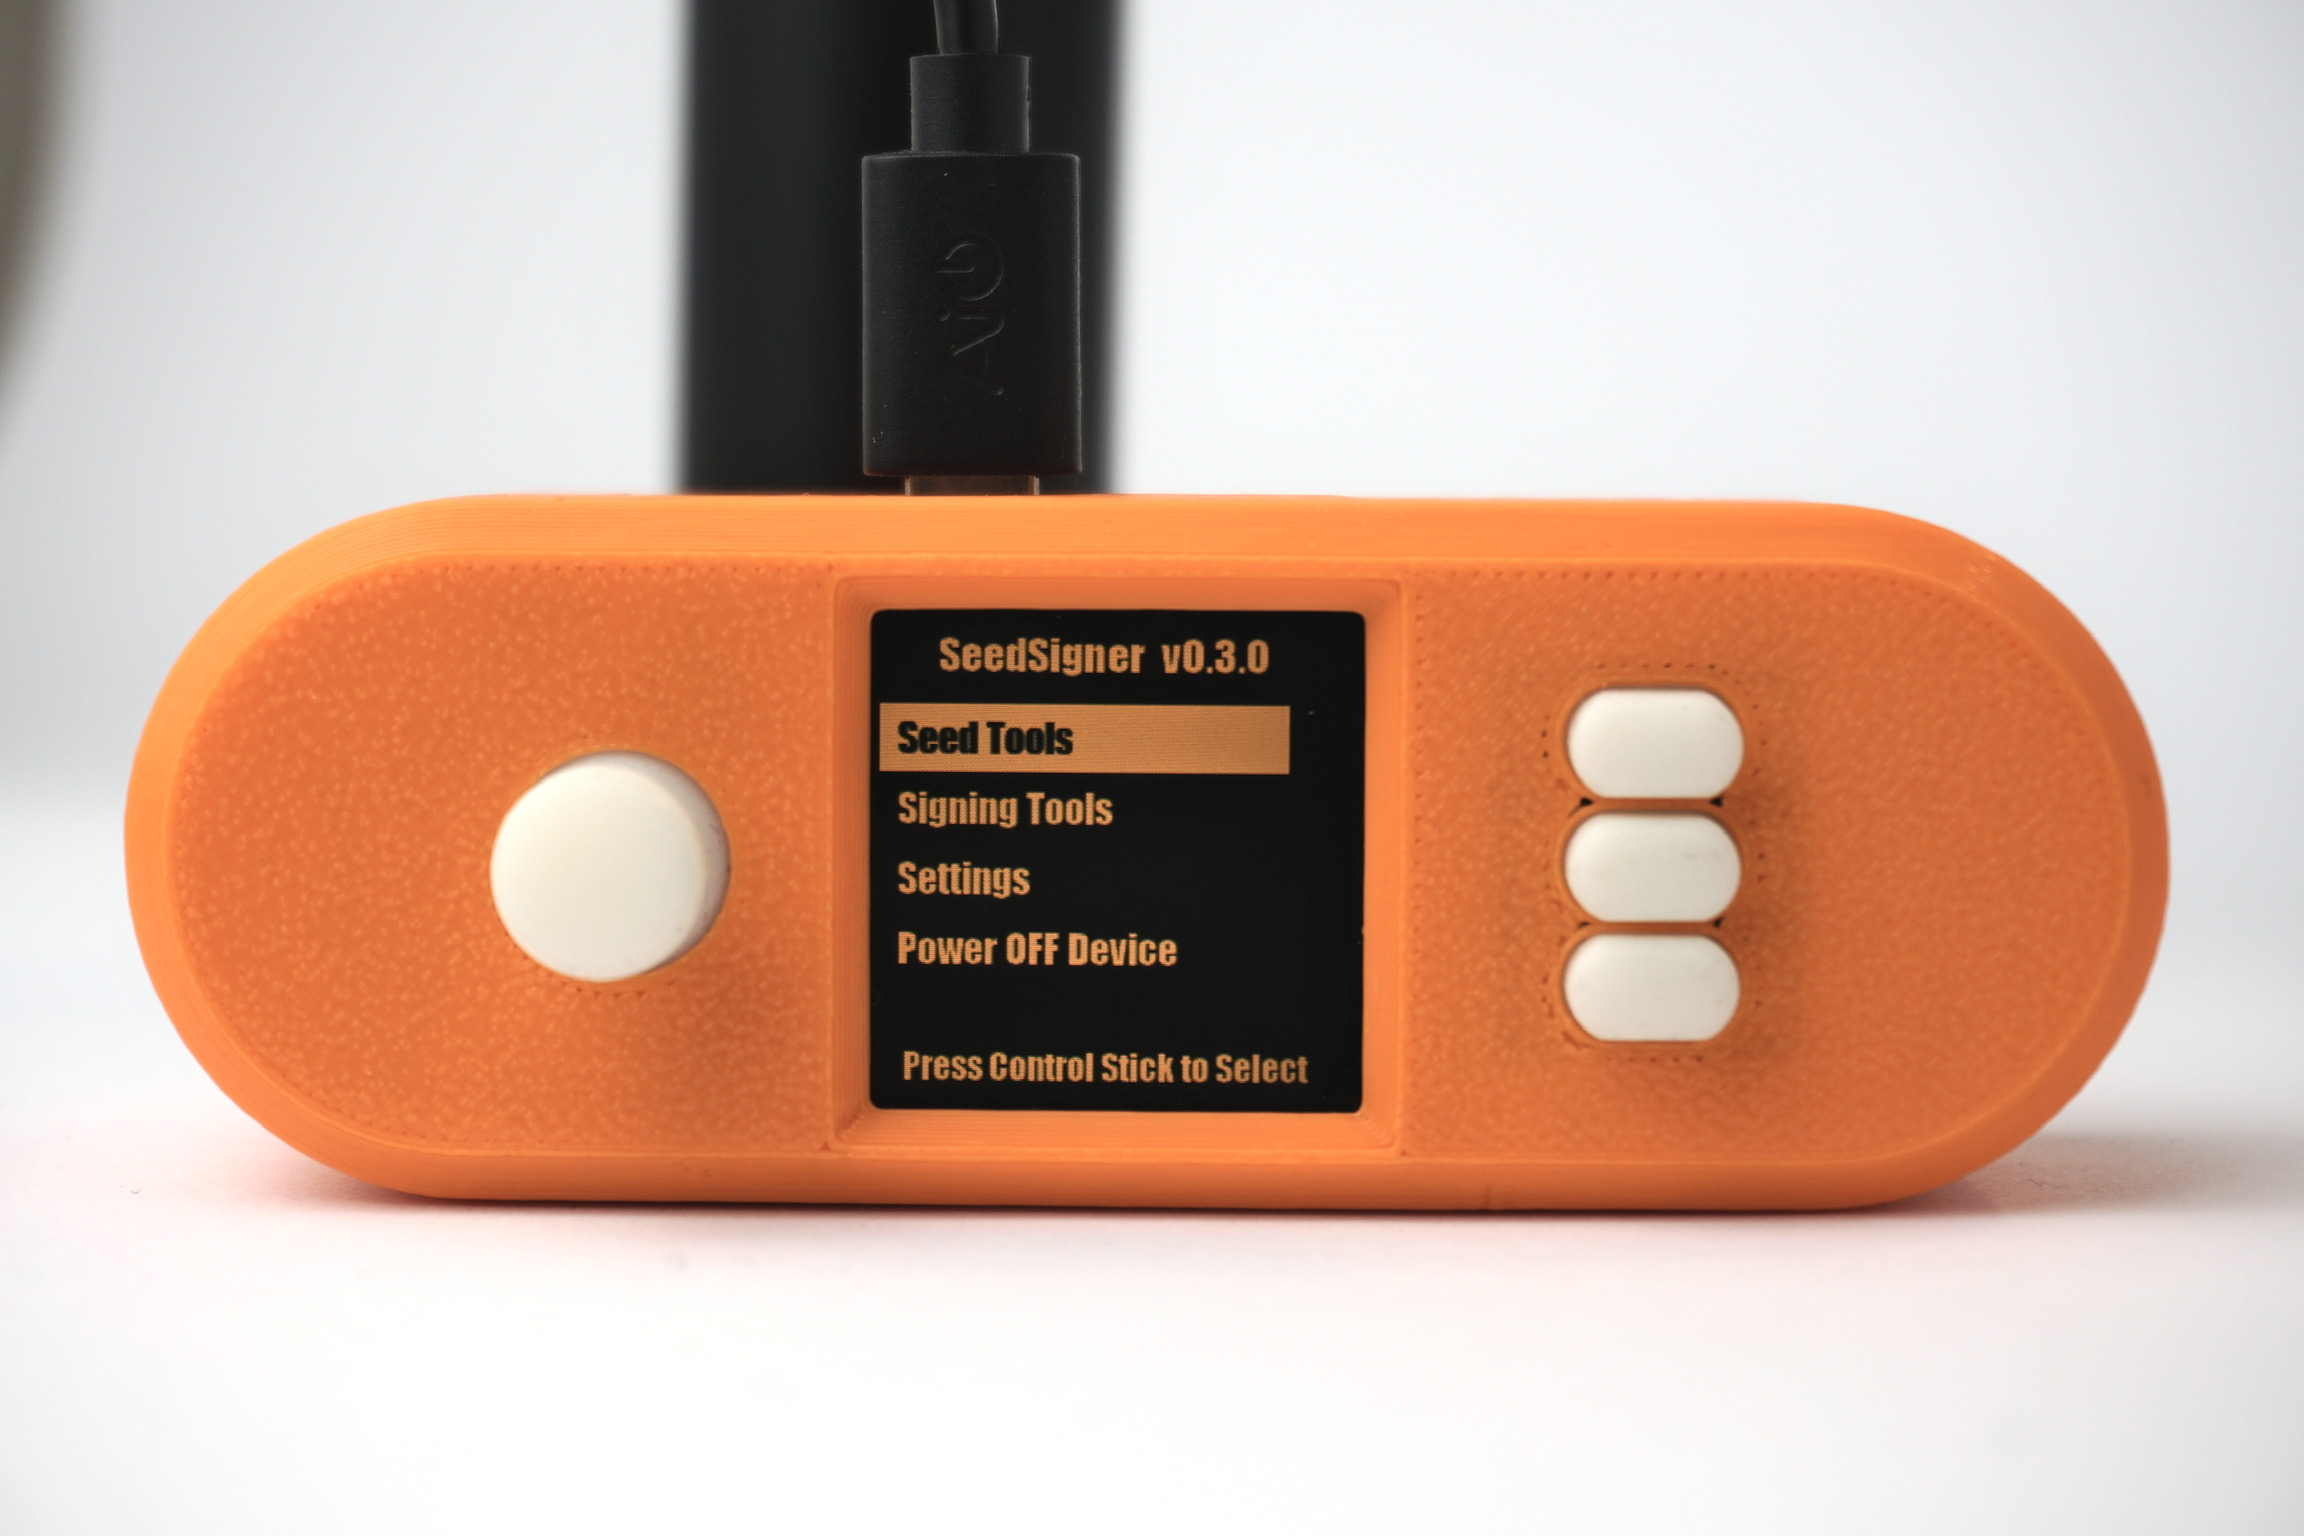
\includegraphics[width=\linewidth]{seedsigner}
  \caption{Seedsigner is an inexpensive open source project which scans the master seed in from a QR code to enable signing. One device can run a quorum based wallet (multisig).}
    \label{fig:seedsigner}
\end{figure}
For higher security it's possible to combine hardware and software wallets (signing devices) to provide a quorum of signatures required to move funds. More exotic still are \href{https://fedimint.org/}{proposals like ``Fedimint''} which allows groups such as families or villages to leverage their personal trust to co-manage Bitcoin. What is not/rarely secure is leaving Bitcoin with a custodian such as an exchange as they simply issue you with an IOU and may abscond. In building toward a proposal for a product in this book it would be simple for us to build a metaverse which users simply paid to use. This is the norm up to now. Representative money would flow around in the metaverse and be changed back like game money at some point. This is not what we wish to promote, so everything will be a variation on ``self-custody'', minimising third party trust for users.
\subsection{Upgrade roadmap}
\subsubsection{Taproot}
`Taproot' is the most recent upgrade to the Bitcoin network. It was first \href{https://lists.linuxfoundation.org/pipermail/bitcoin-dev/2018-January/015614.html}{described in 2018} on bitcoin-dev mailing list, and become \href{https://github.com/bitcoin/bips/blob/master/bip-0341.mediawiki}{BIP-0341} in 2019. It brings improved scripting, smart contract capability, privacy, and Schnorr signatures \cite{schnorr1989efficient}, which are a maximally efficient signature verification method. The network will always support older address types. It is rare to get such a large update to the network, and deployment and upgrade was carefully managed over several months under BIP-0008. Uptake will be slow as wallet manufacturers and exchanges add the feature. It can be considered an \href{https://transactionfee.info/charts/transactions-spending-taproot/}{upgrade in progress (0.3\%)}. Aaron van Wirdum, a journalist and educator in the space describes Taproot in detail in \href{https://bitcoinmagazine.com/technical/taproot-coming-what-it-and-how-it-will-benefit-bitcoin}{an article}.\par
\subsubsection{AnyPrevOut}
\href{https://anyprevout.xyz}{BIP-0118}, is a ``\href{https://en.bitcoin.it/wiki/Softfork}{soft-fork} that allows a transaction to be signed without reference to any specific previous output''. It enables ``Eltoo, a protocol that fulfils Satoshi's vision for nSequence''\par
This is Lightning Network upgrade technology in the main. The Eltoo \href{https://blockstream.com/eltoo.pdf}{whitepaper} or this more \href{https://fiatjaf.alhur.es/ffdfe772.html}{readable explanation} from developer fiatjaf go into detail.\par 
\subsubsection{CheckTemplateVerify}
\href{https://utxos.org/}{BIP-0119} is ``a simple proposal to power the next wave of Bitcoin adoption and applications. The underlying technology is carefully engineered to be simple to understand, easy to use, and safe to deploy''. At it's most basic it is a constructed set of output hashes, creating a Bitcoin address, which if used, can only be spent under certain defined conditions. This is a feature called `covenants'. It enables a feature called `vaults' which provides \href{https://github.com/jamesob/simple-ctv-vault/blob/7dd6c4ca25debb2140cdefb79b302c65d1b24937/README.md}{additional safety features} for custodians. There is currently \href{https://blog.bitmex.com/op_ctv-summer-softfork-shenanigans/}{some debate about the activation process}, and the feeling is that it won't happen (soon).
\subsubsection{Blind merge mining}
BIP-0301 allows `other' chains transactions to be mined into Bitcoin blocks, and for miners to take the fees for those different chains, without any additional work or thoughts by the miners. This is also a prerequisite for Drivechains (mentioned later), and improve Spacechains. In a way this can offer other chains the security model of the Bitcoin network, while increasing fees to miners, which might be increasingly important as the block subsidy falls. This is pretty fringe knowledge \href{https://bitcointalk.org/index.php?topic=1790.msg28696#msg28696}{originally proposed} by Satoshi, but has been refined since and is best explained by \href{https://www.youtube.com/watch?v=xweFaw69EyA}{Paul Sztorc elsewhere}. It is likely an important upgrade in light of the \href{https://www.truthcoin.info/blog/security-budget/}{security budget} of Bitcoin.
\subsubsection{Simplicity scripting language}
\href{https://blockstream.com/simplicity.pdf}{Simplicity} is a proposed contract scripting language which is \href{https://coq.inria.fr/}{`formally provable'}. This would provide a radical upgrade to confidence in smart contract creation. It is \href{https://github.com/ElementsProject/simplicity/blob/pdf/Simplicity-TR.pdf}{work in progress}, and looks to be incredibly difficult to develop in, despite the name. It is more akin to \href{https://en.wikipedia.org/wiki/Assembly_language}{assembly language}. Development has recently slowed, and the proposal requires a soft fork to Bitcoin. The main reason to think it stands a chance of completion vs other \href{https://lists.linuxfoundation.org/pipermail/bitcoin-dev/2022-March/020036.html}{similar proposals} is the powerful backing of \href{https://blockstream.com/}{Blockstream}, one of the main drivers of the Bitcoin ecosystem, run by Adam Back (potential co-creator of Bitcoin). 
\subsubsection{Ossification}
The Bitcoin code is aiming toward so called \href{https://en.wikipedia.org/wiki/Protocol_ossification}{``ossification''}. The complete cessation of development of the feature set. This would provide higher confidence in the protocol moving forward, as long term investors would be somewhat assured that the parameters of the technology would not change, and potentially pressure on the developers would reduce. There's a push to get some or all of the features described above in over the next few year before this happens. As ever this is a controversial topic within the development community. Notably Paul Sztorc, inventor of Drivechain \href{https://www.truthcoin.info/blog/sc-vision/}{feels strongly} that cessation of innovation is a fundamental mistake, while also agreeing that ossification is necessary.
\section{Extending the BTC ecosystem }
The following section are by no means an exhaustive view of development on the Bitcoin network, but it does highlight some potentially useful ideas for supporting metaverse interactions in a useful timeframe.
\subsection{Block \& SpiralBTC}
Block (formally the payment processor ``Square'' is now an umbrella company for several smaller 'building block' companies, all of which are major players in the space. Block itself is now part of the \href{https://www.w3.org/Consortium/Member/List}{W3C web consortium}, so they will be driving a new era of standards in distributed identity and value transfer.\par
SpiralBTC, formally `Square Crypto' (a subsidiary of Square) is funding development in Bitcoin and Lightning. Their main internal product is the \href{https://spiral.xyz/blog/what-were-building-lightning-development-kit/}{Lightning Development Kit} (LDK). This promising open source library and API will allow developers to add lightning functionality to apps and wallets. It is a useful contender for our metaverse applications. They also fund external open source development.\par
\subsection{BTCPayServer}
BTCPayServer is one of the recipients of a Spiral grant. It is a self hosted Bitcoin and Lightning payment processor system which allows merchants, online, and physical stores and businesses to integrate Bitcoin into their accounting systems. It might seem that if one were to use Bitcoin then a simple address published on a website might be enough, but this is far from privacy best practice. Using a single address creates a data point which allows external observers to tie all interactions with a given point of sale to all of the customers, and onward to all of their other transactions through the public ledger. Since we seek to employ cyber security best practice will avoid \href{https://en.bitcoin.it/wiki/Address_reuse}{the issues with address reuse}. Each Bitcoin address should be used just once. This is fine as there's essentially an \href{https://privacypros.io/btc-faq/how-many-btc-addresses}{unlimited number} of addresses.\par
In a metaverse application there is no website to interact with, but fortunately BTCPayServer is completely open source and extensible, has a strong support community, \href{https://docs.btcpayserver.org/API/Greenfield/v1/#operation/Invoices_CreateInvoice}{and an API} which could be integrated with a virtual world application. 
BTCPayServer supports the \href{https://docs.btcpayserver.org/LightningNetwork/}{main three} distributions of Lightning but would potentially need extending in order to work with newer technology like RGB or Omnibolt.
\section{Lightning (Layer 2)}
Lightning was a 2016 proposal by Poon and Dryja \cite{poon2016bitcoin}, and is a method for networks of channels of Bitcoin between parties, which can transfer value. The main public network is a community driven liquidity pool which enables scaling and speed improvements for the Bitcoin network. It makes Bitcoin more like money \cite{divakaruni2022lightning}. As with Bitcoin base chain there are multiple standards and approaches, but within Lightning these are not necessarily cross compatible with one another, resulting in several Lightning networks. This is to our advantage as innovation is possible within these smaller networks. It is mainly `powered' by \href{https://plebnet.wiki/wiki/Main_Page}{thousands of volunteers} who invest in hardware and lock up their Bitcoin in their nodes, to facilitate peer-to-peer transactions. Zebka et al. found that although the network is ``fairly decentralised'' it is more recently skewing to larger more established nodes \cite{zabka2022short}. Though this is a grassroots technology the nature of the design means it can likely be trusted for small scale commercial applications.\par
The following text is from \href{https://medium.com/@johncantrell97?p=5cc72f2c664}{John Cantrell}, an engineer who works on Lightning.\par

\textit{``The Lightning Network is a p2p network of payment channels. A payment channel is a contract between two people where they commit funds using a single onchain tx.  Once the funds are committed they can make an unlimited amount of instant \& free payments over the channel.
You can think of it as a tab where each person tracks how much money they are owed.  Each time a payment is made over the channel both parties update their record of how much money each person has.  These updates all happen off-chain and only the parties involved know about them. When it`s time to settle up the two parties can take the final balances of the channel and create a channel closing transaction that will be broadcast on chain.  This closing transaction sends each party the final amounts they are owed. This means for the cost of two on-chain transactions (the opening and closing of the channel) two parties can transact an unlimited number of times and the overall cost of each transaction approaches zero with every additional transaction they make over the channel. Payment channels are a great solution for two parties to transact quickly and cheaply but what if we want to be able to send money to anyone in the world quickly and cheaply?  This is where the Lightning Network comes into play, it`s a p2p network of these payment channels. This means if Alice has a payment channel with Bob and Bob has a channel with Charlie that Alice can send a payment to Charlie with Bob`s help. This idea can be extended such that you can route a payment over an arbitrary number of channels until you can reach the entire world. Routing a payment over multiple channels uses a specific contract called a Hash Time Locked Contract (HTLC).  It introduces the ability for Bob and any other nodes you route through to charge a small fee.  These fees are typically orders of magnitude smaller than onchain fees. This all sounds great but what if someone tries to cheat? I thought the whole point of Bitcoin was that we no longer had to trust anyone and it sure sounds like there must be some trust in our channel partners to use the Lightning Network? The contracts used in Lightning are built to prevent fraud while requiring no trust.  There is a built-in penalty mechanism where if someone tries to cheat and is caught then they lose all of their money.  This does mean you need to be monitoring the chain for fraud attempts.''}

%\href{https://twitter.com/marcrjandrew/status/1478052587387568130}{Five facts about lightning}
Lightning is a key scaling innovation in the bitcoin network at this time. It is seeing rapid development and adoption (Figure \ref{fig:lightningAdoption}). The popular payment app ``Cash App'' integrates the technology, and `Lightning Strike' services the USA, El Salvador, and Argentina with zero exchange and transmission fees.
\begin{figure}
  \centering
    \includegraphics[width=\linewidth]{lightningAdoption}
  \caption{\href{https://www.research.arcane.no/the-state-of-lightning}{Arcane research lightning adoption overview}.}
  \label{fig:lightningAdoption}
\end{figure}
It allows for unbound scaling of transactions (millions of transations per second compared for instance to around 45,000 TPS in the VISA settlement network). Transaction costs are incredibly low, and the transaction speed virtually instantaneous.\par
The most popular lightning software is \href{https://github.com/lightningnetwork/lnd#readme}{LND} from Lightning Labs or \href{https://github.com/ElementsProject/lightning}{C-Lightning} from Blockstream. The software can be run on top of any Bitcoin full node, in a browser extension with a limited node, in a mobile app as a client or a server, or a hybrid such as the Greenlight server \href{https://medium.com/breez-technology/get-ready-for-a-fresh-breez-multiple-apps-one-node-optimal-ux-519c4daf2536}{used by Breez wallet}. Different trust implications flow from these choices.
\subsection{Micropayments}
Possibly the most important affordance of the Lightning network is the concept of micropayments, and streaming micropayments. It is very simple to transfer even \href{https://satsymbol.com/}{one satoshi} on Lightning, which is one hundred millionth of a bitcoin, and a small fraction of a penny. This can be a single payment, for a very small goods or service, or a recurring payment on any cadence. This enables streaming payments for any service, or for remittance, or remuneration. These use cases likely have enormous consequences which are just beginning to be explored. Integration of this capability into metaverse applications will be explored later.
\subsection{BOLT12 and recurring payments}
\href{https://bolt12.org/}{BOLT12} is a new and developing 'standard' which simplifies and extends the capability of the network for recurring payments, but can negotiate single payments too. The example keyring QR code seen in Figure \ref{fig:bolt12keyring} can be scanned to send single or recurring payments securely and anonymously to the holder.
\begin{figure}
  \centering
    \includegraphics[width=\linewidth*\real{0.5}]{bolt12keyring}
  \caption{\href{https://twitter.com/SeedMint21/status/1518934554840600579}{A key fob with a Bolt12 QR code}}
  \label{fig:bolt12keyring}
\end{figure}
%\subsubsection{Physical Cards}
%\href{https://www.coincorner.com/theboltcard}{Coincorner Bolt card} is an NFC enabled LNURL lightning source which allows tap to pay at lightning enabled vendors. \href{https://www.coindebit.io/}{Coindebit} meanwhile is a VISA card which can be ``charged'' with USD over Lightning. 
\subsection{LNURL-auth}
\href{https://lightninglogin.live/learn}{What is LNURL-auth?}
\textit{``LNURL-auth is a generic authentication protocol. It authenticates the user using digital signatures, which means that the user needs to have a public-private key pair. Thanks to the rising popularity of lightning wallets, more and more users are in possession of and have easy access to such keys. Consequently, users are identified by their public keys, nothing else. The protocol does not require any other identifying information such as passwords, emails, usernames, or similar.''}\par
\textbf{\href{https://github.com/fiatjaf/lnurl-rfc/blob/legacy/lnurl-auth.md}{LNURL-auth} may be able to service all of our user management via LNBits}.
\subsection{LNBits}
LNBits is an open source, extensible, Lightning `source' management suite. It is self hosted, and can connect to a variety of Lightning wallets, further abstracting the liquidity to provide additional functionality to network users. Remember that all of these tools run without a third party, on a £200 setup, hosted at home or within a business. The best way to explore this is to describe \textit{some} of the plugins. 
\begin{itemize}
\item ``\href{https://github.com/lnbits/lnbits-legend#lnbits-v03-beta-free-and-open-source-lightning-network-walletaccounts-system}{Accounts System}; Create multiple accounts/wallets. Run for yourself, friends/family, or the whole world!''
\item \href{https://github.com/lnbits/lnbits-legend/tree/quart/lnbits/extensions/events#events}{Events plugin} allows QR code tickets to be created for an event, and for payments to be taken for the tickets.
\item \href{https://github.com/lnbits/lnbits-legend/tree/quart/lnbits/extensions/jukebox#jukebox}{Jukebox} creates a Spotify based jukebox which can be deployed online or in physical locations.
\item \href{https://github.com/lnbits/lnbits-legend/tree/quart/lnbits/extensions/livestream#dj-livestream}{Livestream} provides an interface for online live DJ sets to receive real-time Lightning tips, which can be split automatically in real-time with the music producer.
\item \href{https://github.com/lnbits/lnbits-legend/tree/quart/lnbits/extensions/tpos#tpos}{TPoS}, \href{https://github.com/arcbtc/LNURLPoS#lnurlpos}{LNURLPoS} \& \href{https://github.com/lnbits/lnbits-legend/tree/quart/lnbits/extensions/watchonly#watch-only-wallet}{OfflineShop} support online \href{https://rapaygo.com/}{and offline} point of sale (Figure \ref{fig:LnBitsPoS}).
\item \href{https://github.com/lnbits/lnbits-legend/tree/quart/lnbits/extensions/paywall#paywall}{Paywall} creates web access control for content. 
\item \href{https://github.com/LightningTipBot/LightningTipBot#lightningtipbot-}{LightningTipBot} is a custodial Lightning wallet and tip handling bot within the popular on Telegram instant messenger service.
\end{itemize}
\begin{figure}
  \centering
    \includegraphics[width=\linewidth*\real{0.8}]{LnBitsPoS}
  \caption{Two of the many \href{https://rapaygo.com/}{prebuilt} and \href{https://github.com/arcbtc/LNURLPoS}{kit} options for Lightning `point of sale'}
  \label{fig:LnBitsPoS}
\end{figure}
Together these plugins are incredibly useful primitives which are likely to be translatable to a multi party metaverse application. A proposal for building a more specific plugin along these lines is detailed later.\par
\textbf{LnBits is capable of backing every object in a metaverse scene as an economic actor, with a key which is compatible with Nostr. This makes it the best choice and it will likely form the core of the proposed metaverse stack.}
\subsection{Etleneum}
Etleneum is a centralised smart contract platform built around Lightning invoices. It is most notable as a sign of things to come. There are \href{https://etleneum.com/#/contracts}{many small contracts} available to try on the site, such as a \href{https://etleneum.com/#/contract/c8w0c13v75}{simple market} for moving value between lightning and Bitcoin layer 1, or this \href{https://simple-auction.etleneum.com/}{simple auction}.  Contracts are able to operate on data drawn from the wider web, and automatically send and receive lightning payments based on conditional states. It should be viewed as an experiment which allows tinkering in smart contracts, and therefore potentially useful for the software proposed in the final section. There are \href{https://notgeld.medium.com/lightning-network-computation-layer-27c7ba81a214}{suggestions} that this approach might (with some work) allow layer 3 computation more like Ethereum etc.
\subsection{Message passing}
It is possible to pass data alongside lightning payments, routing messages between parties across the global network. This means that a host of other applications can inherit the privacy and censorship resistance of the Lightning network. First amongst these has been simple message passing and group messenger clients such as Sphinx and Juggernaut. To be clear, this is considered by some to be a misappropriation of the function of the network. Once more developed use case has been demonstrated by the Impervious development team; they use the message passing capability to negotiate a virtual private network between two parties, using open source software. This allows a secure side channel between internet IP addresses to be opened without a trusted third party. This in itself is a much sought after function of privacy minded networking, and the basis for much of their Impervious browser feature set. 
\section{Liquid federation (layer 2)}
Liquid is an implementation on Blockstream \href{https://elementsproject.org/}{Elements}, and is itself part of the open source development contribution of Blockstream, the company started by Adam Back (of hashcash fame) and nearly a dozen other early cypherpunks and luminaries.\par 
The Liquid side chain network, and it's own attendant Lightning layer 2, is a fork of Bitcoin with different network parameters. In liquid the user of the network `pegs' into the Bitcoin network, swapping tokens out from BTC to L-BTC (this can of course mean very small subunits of 1 Bitcoin). Once tokens have been `locked' and swapped to Liquid the different network parameters used in the fork allow a different trust/performance trade-off. Liquid is fast on the L1 chain, cheaper to use at this time, and more private. The consensus achieved on this side chain network is faster because it is a far smaller group of node operators. The next block to be written to the side chain is chosen by a node operated by a member of a federation of dozens of major contributors to the Bitcoin technology space. These `trusted' nodes all check one another's security and network operations, meaning that the network is as secure as the aggregate of the trust placed in half of the membership at any one time. There are
\href{https://bitcoinmagazine.com/business/bitcoin-liquid-network-gains-six-new-federation-members}{still dozens} of major companies, development teams, and individual actors, with significant reputational investment.\par
``Federation members contribute to the Liquid Network's security, gain voting rights in the board election and membership process, and provide valuable input on the development of new features. Members also benefit from the ability to perform a peg-out without a third party, allowing their users to convert between L-BTC and BTC seamlessly within their platform.''\par
Crucially for our purposes here Liquid allows tokenised asset transfer. Anyone \href{https://docs.blockstream.com/liquid/developer-guide/developer-guide-index.html#issued-assets}{can issue} an asset on Liquid. Such transfers of assets may be orders of magnitude cheaper than on chain Bitcoin transactions, but still potentially orders of magnitude more expensive than a simple Lightning transaction of value on the Bitcoin network. \par 
Blockstream plan to add arbitrary (user generated) token support to their `Core Lightning' implementation at some point. This would be a very strong choice for specific use cases within an economically enabled metaverse application. When participants wish to `cash out' of the Liquid network they must do this through one of the federation members who activate the other side of the `two-way peg', dispensing the equivalent amount of Bitcoin. This is transparently handled through Blockstream's ``green wallet''.\par
All of this has the advantage of a far lower energy footprint compared to the main chain, but it's not quite ready with a full suite of affordances. \par
The Liquid network is being used as the underlying asset for a novel new global financial product. El Salvador are working with Blockstream to issue a nation state backed bond. 
\section{Bitcoin Layer 3}
Increasingly important features of modern blockchain implementations are programmability through smart contracts, and issuance of arbitrary tokens. Assigning a transaction to represent another thing like an economic unit, energy unit, or real world object, and operating on those abstractions within the chain logic. Chief among these use cases are stablecoins such as Tether, which are pegged to national currencies and described in the next section. Bitcoin has always supported very limited contracts called scripts, and stablecoin issuance has existed in Bitcoin since 
\href{https://www.omnilayer.org/}{Omni Layer}. Omni was the first issuer of Tether, but more recently these important features have passed to other layer one chains. This year is likely to see the \href{https://www.hiro.so/blog/bitcoin-ecosystem-a-guide-to-programming-languages-for-bitcoin-smart-contracts}{resurgence of this capability} on Bitcoin, which of course benefits from a better security model. Once again, there is a stong assertion by some that \href{https://lists.linuxfoundation.org/pipermail/bitcoin-dev/2022-April/020227.html}{this isn't even possible}. The debate is complex and unresolved.\par 
In order to properly understand the use of Bitcoin based technologies in metaverse applications it is necessary to examine what these newer `layer 3' ideas might bring. 
\subsection{LNP/BP and RGB}
\href{https://giacomozucco.com/layers-before-bitcoin}{LNP/BP} is a non profit standards organisation in Switzerland which contributes to open source development of Bitcoin layer 3 solutions into the Lightning protocol, and Bitcoin protocol (LNP/BP). One of the core product developments within their work is the `RGB' protocol, which is somewhat of a meaningless name, evolved from ``coloured coins'' which were an early tokenised asset system on the Bitcoin network. RGB represents red, green, and blue. The proposal is built upon research by \href{https://petertodd.org/2016/commitments-and-single-use-seals}{Todd} and \href{https://giacomozucco.com/#intro}{Zucco}. RGB is regarded as arcane Bitcoin technology, even within the already rarefied Bitcoin developer communities. Zucco provides the \href{https://bitcoinmagazine.com/culture/video-interview-giacomo-zucco-rgb-tokens-built-bitcoin}{following explanation}: \par
\textit{``When I want to send you a bitcoin, I will sign the transaction, I will give the transaction only to you, you will be the only one verifying, and then we’ll take a commitment to this transaction and that I will give only the commitment to miners. Miners will basically build a blockchain of commitments, but without the actual validation part. That will be only left to you. And when you want to send the assets to somebody else, you will pass your signature, plus my signature, plus the previous signature, and so on.''}\par
This is non-intuitive explanation of Todds `single-use-seals', applied to Bitcoin, with the purpose of underpinning arbitrary asset transfer secured by the Bitcoin network. In this model the transacting parties are the exclusive holders of the information about what the object they are transferring actually represents. This primitive can (and has) been expanded by the LNP/BP group into a concept called `client side validation'. 
It's appropriate to explain this concept several times from different perspectives, because this is potentially a profoundly useful technology for metaverse applications.\par
\begin{itemize}
\item A promise is made to spend a multi output transaction in the future. This establishes the RGB relationships between the parties.
\item One of the pubkeys to be spent to is known by both parties.
\item The second output is unknown and is a combination of the hash of the state, and schema, from the operation which has been performed.
\item When the UTXO is spent the second spends pubkey can be processed against the shared data blob to validate the shared state in a two party consensus  (sort this out, it's nonsense).
\item This is now tethered to the main chain. Some tokens from the issuance have gone to the recipiant, and the remainder have gone back to the issuer. More tokens can be issued in the same way from this pool. 
\item A token schema in the blob will show the agreed issuance and the history back to the genesis for the token holder. 
\item The data blob contains the schema which is the key to RGB functions and the bulk of the work and innovation. 
\item Each issuance must be verified on chain by the receiving party. 
\end{itemize} 
This leverages the single-use-seal concept to add in smart contracts, and more advanced concepts to Bitcoin. Crucially, this is not conceptually the same as the highly expressive `layer one' chains which offer this functionality within their chain logic. In those systems there is a globally available shared consensus of `state'. In the LNP/BP technologies the state data is owned, controlled, and stored by the transacting parties. Bitcoin provides the crytographic external proof of a state change in the event of a proof being required. This is an elegant solution in that it takes up virtually no space on the blockchain, is private by design, and is extensible to layer 2 protocols like Lightning.\par
This expanding ecosystem of client side verified proposals is as follows:
\begin{itemize}
\item RGB smart contracts
\item RGB assets are fungible tokens on Bitcoin L1 and L2, and non fungible Bitcoin L1 (and somewhat on L2).
\item Bifrost is an \href{https://github.com/LNP-BP/presentations/blob/master/Presentation slides/Bifrost.pdf}{extension} to the Lightning protocol, with it's own Rust based node implementation, and backwards compatibility with other nodes in the network. This means it can transparently participate in normal Lightning routing behaviour with other peers. Crucially however it can also negotiate passing the additional data for token transfer between two or more contiguous Bifrost enabled parties. This can be considered an additional network liquidity problem on top of Lightning, and is the essence of the ``Layer 3'' moniker associated with LNP/BP. It will require a great number of such nodes to successfully launch token transfer on Lightning. As a byproduct of it's more `protocol' minded design decisions Bifrost can also act as a generic peer-to-peer data network, enabling features like Storm file storage and Prometheus.
\item \href{https://www.aluvm.org/}{AluVM} is a RISC based virtual machine (programmable strictly in assembly) which can execute Turing complete complex logic, but only outputs a boolean result which is compliant with the rest of the client side validation system. In this way a true or false can be returned into Bitcoin based logic, but be arbitrarily complex within the execution by the contract parties.
\item Contractum is the proposed smart contract language which will compile the RGB20 contracts within AluVM (or other client side VMs) to provide accessible layer 3 smart contracts on Bitcoin. It is a very early proposal at this stage.
\item  Internet2: ``Tor/noise-protocol Internet apps based on Lightning secure messaging
\item Storm is a lightly specified escrow-based bitcoin data storage layer compliant with Lightning through Bifrost.
\item Prometheus is a lightly specified multiparty high-load computing framework.
\end{itemize}
Really, any compute problem can be considered applicable to client side validation. In simplest terms a conventional computational problem is solved, and the cryptographically verifiable proof of this action, is made available to the stakeholders, on the Bitcoin ledger.\par 
Less prosaically, at this stage of the project the more imminent proposed affordances of LNP/BP are described in `schema' \href{https://github.com/LNP-BP/LNPBPs}{on the project github}. The most interesting to the technically minded layperson are:
\begin{itemize}
\item \href{https://github.com/LNP-BP/LNPBPs/blob/master/lnpbp-0020.md}{RGB20} fungible assets. This could be stablecoins like dollar or pounds representation. This is a huge application area for Bitcoin, and similar to Omni, which will also be covered next.
\item \href{https://github.com/LNP-BP/LNPBPs/blob/master/lnpbp-0021.md}{RGB21} for nonfungible tokens and ownership rights. In principle BiFrost allows these to be transferred over a future version of the Lightning network, significantly lowering the barrier to entry for this whole technology. This is slated for release later in the year.
\item \href{https://github.com/LNP-BP/LNPBPs/issues/29}{RGB22} may provide a route to identity proofs. This is covered in detail later.
\end{itemize}
Federico Tenga is CEO of `Chainside' and an educator and consultant in the space. He has written an up-to-date \href{https://medium.com/@FedericoTenga/understanding-rgb-protocol-7dc7819d3059}{``primer''}, which is still extremely complex for the uninitiated, but does capture how the RGB token transfer system works. That medium article also touches on Taro, which is next.
\subsection{Taro}
Taro is an very new \href{https://lightning.engineering/posts/2022-4-5-taro-launch/}{initiative by Lightning Labs} to allow assets to transmit on the Lightning network. It is more similar to RGB above than Omnibolt below. They say: \textit{``Taro enables bitcoin to serve as a protocol of value by allowing app developers to integrate assets alongside BTC in apps both on-chain and over Lightning. This expands the reach of Lightning Network as a whole, bringing more users to the network who will drive more volume and liquidity in bitcoin, and allowing people to easily transfer fiat for bitcoin in their apps. More network volume means more routing fees for node operators, who will see the benefits of a multi-asset Lightning Network without needing to support any additional assets.''}\par
The project has clearly been \href{https://github.com/roasbeef/bips/tree/bip-taro}{under development} by the lead developer at Lightning Labs for some years and seems both \href{https://lightninglabs.substack.com/p/bitcoinizing-the-dollar-and-the-world?s=r}{capable} and mature, though they are obviously following the model of `co-opting' open source ideas (from RGB) to garner venture capital funding. They \href{https://github.com/bitcoin/bips/pull/1298/commits/4daba8c373c777defb48136795382803c137502c}{credit RGB} in the github. More will doubtless be added to this section and it seems a contender for our metaverse purposes, being less broadly ambitious than RGB upon which it's based, but perhaps more focused and implemented. The key feature of Taro seems to be that only the first and last hop in a multi-hop lightning transaction need to support Taro, because of external data validation databases called ``universes''. This is an advance on the RGB proposal. 
The technical specs are now on the \href{https://docs.lightning.engineering/the-lightning-network/taro}{lightning labs web pages}.
\subsection{Slashpay}
Slashpay is a very promising and recent product, and part of a suite of interlinked (Bitcoin compatible) layer 3 ideas. It is \textit{not} a blockchain technology, but it is highly intersectional with Bitcoin. The Synonym suite is advocating what they call the `Atomic Economy', an overarching abstraction of any of the technologies in the space into a single cryptographic key pair, with all the other products nested under it. The suite will be selected and unpacked for metaverse purposes later, but for this section the Slashpay product integrates as a layer three idea, building upon lightning. \par
Slashpay gathers all of the available Lightning invoice and QR code `standards' under an abstracted metastandard with it's own key pair. This allows a negotiation between party and counterparty in code, which settles on agreeable standards for the value transfer. The Slashpay mediation metadata is embedded in the top level Slashtag QR code. Within the Slashpay element of the data is a priority list for the exchange, which can be changed by the user according to their capability and preferences.\par 
The code to support this is in a early stage. There is a minimum viable product which can negotiate between online Lightning nodes. The advantage of the Slashpay method, and the thing that puts it in the layer 3 section, is that in the event of a failed Lightning payment (for whatever reason), the software can then default to the next payment method in it's negotiated list. This would most likely be another (different) Lightning attempt, or a Bitcoin main chain transaction.\par
This technical ecosystem uses a `distributed hash table' to hold and negotiate keys, stored using Hypercore, another external project based on Bittorrent. This is the \href{https://hypercore-protocol.org/protocol/#hyperswarm}{`Hyperswarm DHT'}, which has potential uses elsewhere in the metaverse use cases.\par
There is clearly additional complexity in setting this system up, but once in place it might provide a unified way to scale capability under the evolving standard.  
\subsection{Spacechains}
Spacechains is a \href{https://medium.com/@RubenSomsen/21-million-bitcoins-to-rule-all-sidechains-the-perpetual-one-way-peg-96cb2f8ac302}{proposal} by Ruben Somsen. It is a way to provide the functionality of any conceivable blockchain, by making it a sidechain to Bitcoin. \par
Like RGB described earlier it's a single use seal, but which can be closed by the highest bidder.\par
In a spacechain the Bitcoin tokens are destroyed in order to provably create the new spacechains tokens at a 1:1 value. These new tokens only have worth moving forward within the new chain ecosystem they represent, as they cannot be changed back. They nontheless have the same security guarantees as the bticoin main chain, though with a radically reduced ecological footprint (x1000?), and higher performance. Each `block' in the new chain is a single bitcoin transaction. The high level features are:\par
\begin{itemize}
\item Outsource mining to BTC with only a single tx per block on the main chain.
\item One way peg, Bitcoin is burnt to create spacechain tokens.
\item Allows permissionless chain creation, without a speculative asset.
\item Fee bidding BMM is space efficient and incentive compatible. Miners just take the highest fees as normal.
\item Paul Sztorc raised the idea
\item It's best with a soft fork but possible without
\end{itemize}
The concept is \href{https://vimeo.com/703246895/d89aba6e56}{explained fully} in a recent presentation at Advancing Bitcoin conference.

%\subsection{Drivechain}
%\lipsum[50]
%\subsection{Softchains}
%\lipsum[50] 
\subsection{Statechains, drivechain, softchains} 
There are many \href{https://gist.github.com/RubenSomsen/96505e99dc061d6af6b757ff74434e70}{proposals for layer 2 scaling solutions} for the bitcoin network. Ruben Somsen \href{https://gist.github.com/RubenSomsen/c9f0a92493e06b0e29acced61ca9f49a}{describes Softchains, Stateschains, and Spacechains}, while  \href{https://www.drivechain.info/literature/index.html}{Drivechain is described} by the author Paul Sztorc on the project web pages and is split across \href{https://github.com/bitcoin/bips/blob/master/bip-0300.mediawiki}{BIP-0300} for drivechain and \href{https://github.com/bitcoin/bips/blob/master/bip-0301.mediawiki}{BIP-0301} for a ``blind merge mining'', a soft fork which it's unlikely to get. They are all hypothetical with the exception of sidechains.  

\section{Other chains and networks}
It's useful to make some `honourable mentions' of other options as this technology is moving so fast. These chains are viewed by some as a kind of triage for ideas which might one day find their way into Bitcoin. This is potentially most true of zk rollups which might eventually migrate from privacy and scaling experiments on other chains. This list simply isn't very useful in terms of judging other chains, as they rise and fall so fast. To be clear, there is a fundamental \textit{legal} difference between all of the 15,000 or so attempts at layer 1 chains after Bitcoin, in that they are controlled by a subset of people who have an incentive to lie about the usefulness of the technologies they are invested in. This lack of useful decentralisation has been touched on but is dealt with in detail by Microstrategy CEO Michael Saylor in a \href{https://www.youtube.com/watch?v=mC43pZkpTec}{four hour podcast} with Ai researcher Lex Fridman. It's interesting that Saylor (who is a significant educator in the space) views custodial companies holding Bitcoin on behalf of their clients as Bitcoin layer 3. All of this is new enough that virtually all of it is contested by someone. To demonstrate the difference between Bitcoin as a property vs alt coins as `securities in law' it's useful to see the allocations of tokens to seed investors in some of the newer chains in Figure \ref{fig:messariICO}.

\begin{figure}
  \centering
    \includegraphics[width=\linewidth]{messariICO}
  \caption{Allocations given at the beginning of public blockchain, by Messari.}
  \label{fig:messariICO}
\end{figure}

\subsection{Layer 1 chains}
As the market wanes in 2022 the fragility of tokens other than Bitcoin is being exposed. They are suffering brutal losses. Historically tokens spend around 19 weeks in the top tier of tokens before falling away. Each cycle brings and new crop during the bull market and these invariably don't make it through to the next cycle. There are a few which have longevity and name recognition, but mainly because they amassed enough capital during the early days to play a very long, if somewhat pointless game.
\begin{itemize}
\item Monero is a privacy focused coin with a great deal of credible and competent developer attention. It attracts a lot of criticism precisely because it's anonymity by design makes it perfect for nefarious activity such as drugs markets. Privacy advocates in the space say that total unaccountability of money is a `must have' feature and that \href{https://sethforprivacy.com/posts/dispelling-monero-fud/#introduction}{critiques of the chain} are in bad faith. It's actually arguably the best of the alternatives, having a valid use case  in privacy.
\item Solana is a far more centralised layer 1 proposition which uses a few hundred highly performant nodes to achieve high transaction throughput. The consensus algorithm is the novel \href{https://solana.com/solana-whitepaper.pdf}{``proof of history''} system. Development of the technology has been funded and supported by huge venture capital investment, and even though the chain is quite unreliable it seems that the vested interests of the investors can keep interest going. It is cheaper, and more useful than Bitcoin and Ethereum, but lacks longevity and reliability. It could probably be a database. With that said it is well funded, and fun to use. They have \href{https://solana.com/news/solana-mobile-stack-reveal}{announced a mobile stack} and a first foray into making an android mobile phone to leverage it. This would, they say, allow a whole new model of mobile Web3 interaction.
\item Polkadot is much hyped within the ``crosschain'' protocol community. These chains connect the logic of a smart contract on one chain to that of another. In practice, while it is possible that this is useful for distributed finance products, it seems that chains such as DOT might be promising more than the markets actually want or need. Governance of the token is a DAO like model where staking (locking up) the tokens theoretically controls the direction of the product. Crosschain products like this are a cybersecurity nightmare.
%\item Terra is a relatively new \href{https://assets.website-files.com/611153e7af981472d8da199c/618b02d13e938ae1f8ad1e45_Terra_White_paper.pdf}{ecosystem offering} with a stablecoin, and DeFi built in. It is currently in ascendancy (\$15 in a year) and seems to have a stable and useful underpinning, but is far too new to judge with any certainty. There's more on this in the stablecoin section later.
%\item Avalanche AVAX is a newer, `faster' and more eco friendly DeFi ecosystem which promises returns within it's own framework of permissionless money. It is one of the relative success stories of the DeFi narrative. It's unclear what the value proposition, and sustainability of this token actually are.
\item TRON TRX draws extensive criticism for being founded by \href{https://www.theverge.com/c/22947663/justin-sun-tron-cryptocurrency-poloniex}{Justin Sun}. An huge amount of value transacts on TRON, and it could be argued that this gives it a genuine use case. It's more likely another house of cards.
\item Tezos is a well established player with an early and somewhat battle tested proof of stake mechanism and distributed governance model. It has attracted many high profile partnerships and sponsors, but is primarily seeking to be a store of value token like bitcoin, which exposes the chain to the ``winner takes all'' landscape of digital money. There are some compelling NFT advocates of the technology, which is certainly `greener' and cheaper to use, but the longevity in such an irrational market is uncertain, because it does not seem to have the network effect and growth velocity. 
\item Algorand's ALGO token purports to be a more modern and useful proof of stake value transfer chain. It is fundamentally similar to Tezos.
\item IOTA is noteworthy, interesting, and established concept, with an edge use case. It is a `distributed ledger of the internet of things', the much hyped and clearly extant ecosystem of edge compute, sensors, smart devices etc. The marketing around IOTA correctly identifies it's positioning and potential within this developing technology ecosystem, but it's primary use case is too nascent and too niche, and the implementation itself has drawn (valid) \href{https://medium.com/@neha/cryptographic-vulnerabilities-in-iota-9a6a9ddc4367}{criticism for amateurish cryptography} and a fundamentally centralised model. The concept remains interesting.
\item VeChain is a long established platform with `significant' industry adoption which still doesn't represent it's market capitalisation, usefulness, or future success. It is the most exposed of all the chains to the untruth that immutable global ledgers, of real world assets, somehow protect from fraudulent behaviour. It's perhaps useful, but mainly in a highly automated industry 4.0 environment, with minimal human interaction. 
\item Cardano foundation ADA is one of the more established players and has been developing methodically and slowly. They have made great strides in successfully enabling a provable proof of stake consensus structure. Proof of stake non-the-less has significant problems in that tokens and therefore control inevitably concentrates over time. There is no proposed solution to this. They have working products and partnerships, but perhaps not as many as the market cap of the ecosystem would suggest. 
\item HBAR claims ``third generation'' blockchain technology, with carbon positive, high speed, distributed applications. There are always tradeoffs bound by physical constraints within distributed computing, and Hedera HBAR has been accused of a cryptographic model which is inherently insecure.
\item EOS is one of the early major successes of the ICO funding model in 2017, and they amassed an enormous war chest of bitcoin which they still hold. The onus is on them to deliver some kind of product, and they have the funds to do so, but they probably won't.
\end{itemize}
\subsection{Distributed data storage}
\lipsum
\section{Risks and mitigations}
Looking across the whole sector, this paragraph from the Bank of International Settlement (BIS) \href{https://www.bis.org/publ/arpdf/ar2022e3.htm}{sums everything up}: \par
\textit{``...it is now becoming clear that crypto and DeFi have deeper structural limitations that prevent them from achieving the levels of efficiency, stability or integrity required for an adequate monetary system. In particular, the crypto universe lacks a nominal anchor, which it tries to import, imperfectly, through stablecoins. It is also prone to fragmentation, and its applications cannot scale without compromising security, as shown by their congestion and exorbitant fees. Activity in this parallel system is, instead, sustained by the influx of speculative coin holders. Finally, there are serious concerns about the role of unregulated intermediaries in the system. As they are deep-seated, these structural shortcomings are unlikely to be amenable to technical fixes alone. This is because they reflect the inherent limitations of a decentralised system built on permissionless blockchains.''}\par
This might seem like reason enough to  stop here and wait for proper digital currency (expanded later), but Bitcoin is here now, is likely unstoppable in, and with mitigations in place might have uses if developed properly. Perhaps surprising the same BIS is allowing up to 1\% of bank reserves to be held in crypto assets, including Bitcoin, \href{https://www.bis.org/bcbs/publ/d533.pdf}{according to their June 2022 Basel Committee on Banking Supervision report}.
\subsection{Digital assets}
For digital assets more generally it is useful to look at the recent \href{https://www.whitehouse.gov/briefing-room/presidential-actions/2022/03/09/executive-order-on-ensuring-responsible-development-of-digital-assets/}{``whole government executive order''} signed by President Biden. It is mainly framed in terms of ``responsible innovation, and leadership'' in the new space, is a product of multi agency collaboration, and has been long anticipated. It identifies high level risks, aspirations, and challenges, and strongly hints toward development of a ``digital dollar'' (CBDC, expanded later). The risks sections show how legislators are framing this, so it's useful to break down here.\par
\begin{itemize}
\item Consumer and business protections. This is likely to pertain to custodians and is much needed. Misselling is rife. Security presents a challenge.  
\item Systemic risk, and market integrity are a concern. The legislators clearly worry about contagion risks from the sector.
\item Illicit finance (criminality and sanction busting etc) are a concern, but not particularly front and centre\cite{moser2013inquiry}. Criminality in 2021 was a mere 0.15\% of transactions according to Chainalysis, but this number varies year to year. The US treasury department has recently published a National Risk Assessments for Money Laundering, Terrorist Financing, and Proliferation Financing. This is a comprehensive report and speaks to careful research across the space. It is broken into \href{https://home.treasury.gov/news/press-releases/jy0619}{three parts}. Perhaps surprisingly, while they do see activity in these areas, they do not rate the risk as very significant. Cash remains the main problem for illicit funding. There is some talk that the nature of public blockchain analysis allows greater oversight of these tools and that this is to the advantage of government and civil enforcement agencies.
\item Highlighting the need for international coordination suggests they are mindful of jurisdictional arbitrage. 
The partial regulatory capture of these technologies, where activity flows to globally more lenient legislative regimes, continues to be a concern. Many of the centralised exchanges for instance are located in tax havens such as Malta. As the world catches up with these products it is likely that this will be smoothed out.
\item Climate goals, diversity, equality and inclusion are mentioned. It seems that the ``environment'' aspect of ESG is more important then ``social'' and ``governance'' at this time.
\item Privacy and human rights are mentioned.
\item Energy policy is highlighted, including grid management and reliability, energy efficiency incentives and standards, and sources of energy supply.
\end{itemize}
A recent proposed \href{https://bitcoinmagazine.com/business/heres-whats-in-senator-lummis-bitcoin-bill}{bi-partisan bill in the USA} will likely lead global law in digital assets if it is passed later this year. It encourages the use of Bitcoin as a medium of exchange by applying a tax exemption on transactions of less than \$200. The issue of whether an asset is a commodity or a security is left to a couple of major government agencies to unpick, with corresponding reporting requirements. Crucially for this document the draft bill regards both Bitcoin and Ethereum as sufficiently decentralised to qualify as commodities, meaning they would enjoy more lenient oversight. Exchanges will be required to do far more reporting, and would be penalised for trading against their customers. DOAs and DeFi are the big potential losers. In a maddening twist the Office of Government Ethics in the USA has banned anyone who owns digital assets from working on the legislation. This is an exceptional move and likely to result in poorly crafted laws in the first instance.
\subsection{Bitcoin specifically}
\noindent In addition it's useful for this document to focus more on the technical challenges to the Bitcoin network.\par
\begin{itemize}
\item The block reward is reduced every 4 years (epochs). This means a portion of the mining reward is trending to zero, and nobody knows what effect this will have on the incentives for \href{https://www.truthcoin.info/blog/security-budget-ii-mm/}{securing the network} through proof of work \cite{carlsten2016instability}. It is increasingly \href{https://cryptostackers.substack.com/p/bitcoin-is-not-a-store-of-value?sd=pf&s=r}{being discussed} as the major eventual problem for the network.
\item Stablecoins are a vital transitional technology (described later) but do not meaningfully exist yet on the Bitcoin network. This may change.
\item Bitcoin lacks privacy by design. All transactions are publicly viewable. This is a major drag to the concept of BTC as a money. Upgrade of the network is possible, and has indeed been achieved for a Bitcoin fork called Litecoin \cite{fuchsbauer2019aggregate}. 
\item The Lightning network (described later) has terrible UX design at this time. 
\item The basic `usability' of the network is still poor in the main. Any problems which users experience demand a steep learning curve and risk loss of funds. There is obviously no technical support number people can call. 
\item Only around one billion unspent transactions can be generated a year on the network. This means that it might become impossible for everyone on the planet to have their own Bitcoin address (with it's associated underpinning UTXO).  
\item Chip manufacture is concentrated in only a few companies and countries, as identified by Matthew Pines. He also identifies the \href{https://www.btcpolicy.org/#Research}{following points}
\item Potential constraints on monetary policy flexibility.
\item Future protocol changes.
\item Unanticipated effects on the domestic and international energy system.
\item Vulnerability to adversary attacks.
\item Mining tends toward economy of scale concentration. Many are already on their \href{https://bitcoinfibre.org/}{own specialised network} to connect to one another.
\item Future hard forks. There will doubtless be pressure to fork the code to add inflation, or ESG mitigations, or to fix the UNIX clock issue in 2106. Each fork is a risk.
\item Other unknown, unanticipated risks given Bitcoin’s limited 13-year history.
\end{itemize} 


%\subsection{Crime and santion busting}
%


\chapter{Money in the real world}
It is necessary here to briefly examine what money actually is in the world outside of metaverses, so we can understand it in the context of a virtual global space. In the previous section Bitcoin can be viewed in a couple of different lights. As a self custody digital bearer asset it can be viewed as `property', like gold, i.e. not a liability on someone else's asset sheet. Indeed this has long been one of the assertions of the community and it finds favour in law, \href{https://www.regulationasia.com/shanghai-court-says-bitcoin-is-protected-by-law-as-virtual-property/}{possible most ironically in China} which of course banned mining. `Money' though is a far more \href{https://www.bankofengland.co.uk/knowledgebank/what-is-money}{slippery concept} to grasp. It seems very likely that Bitcoin is evolving as a ``base money'', and it's important to define that, but there are many other kinds of money within the online world which can potentially transfer value within virtual social spaces.
\section{Defining money}
Money is an economic good, that is generally accepted as a medium of exchange. This simple and specific description doesn't do justice to the complexity of everything that humans consider to be money. Even the Encyclopaedia Britannica strays from this immediately in their definition:\par
\textit{``money, a commodity accepted by general consent as a medium of economic exchange. It is the medium in which prices and values are expressed; as currency, it circulates anonymously from person to person and country to country, thus facilitating trade, and it is the principal measure of wealth.''}. \\
In which it can be seen that the principle measure of wealth might not be money at all, but rather property, credit, etc. So are these things money? Is a promise on a ledger money? The assertion at the top of this section is challenged by different schools of economic thinking. Global debt is around an order of magnitude larger than base money, and most wealth is stored in illiquid land/built environment (some \$300T), and yet the system seems to work fine. The debt theory of money offered by anthropologist David Graeber suggests that money is an abstraction of barter, and thereby `credit', but credit clearly pre-dates money, and needs no barter, commodity, intermediary nor underlying asset \cite{homer1996history}. This suggests that money is something slightly different.\par
Money seems to have evolved for two principle purposes; trade outside of a village context, and inheritance \cite{szabo2002shelling}. In doing this it somewhat replaced and augmenting `credit', which as said above, was a promise between parties based on future actions, and likely as old as rudimentary language itself.\par
Money can be divided into two categories, which are fungible (interchangeable) from the point of view of the users. Base money is `commodity' money which is backed by assets, or tangible physical (or digital) goods through the actions of a central bank ledger, and is around \$30-\$40T. Everything else is `fiduciary media' \cite{selgin1996defense}.\par
All fiduciary money is credit but not all credit is fiduciary money. Nobody knows the extent of the global supply of fiduciary media. It encapsulates all the new digital money platforms like PayPal, gift cards, offshore accounts and all manner of other vehicles, and is thought to be many tens of trillions of pounds. This somewhat muddies the waters since money that is backed by `something' blends away into money which cannot reasonably be assayed. This in turn undermines the assertion that money is backed. It seems that a combination of available raw materials and labour, central banks and their associated political structures \cite{barsky1987fisher}, and global markets drive the value of money up and down relative to ``stuff'' in the shops. This manifests as `inflation', which is `possibly' the effect of not pegging money to an asset such as silver, or gold as in the past \cite{hall2009inflation}. While the gross drivers of inflation seems to be accepted and understood, nobody \href{https://www.dailymail.co.uk/news/article-10966165/Jerome-Powell-admits-understand-better-little-understand-inflation.html}{seems very sure} how the \href{https://www.bloomberg.com/opinion/articles/2022-08-19/this-economy-is-proving-too-complicated-for-economists}{various aspects interact}.It may be that central banks actually have no decent response to global monetary pressures and are overdue a paradigm shift, as \href{https://www.ft.com/content/2d79d153-fffa-4441-b79f-0a808a51108f}{explained by Daniela Gabor} (Professor of economics and macrofinance at UWE Bristol):\\ 
\textit{``...last stage of a central banking paradigm, when it implodes under the contradictions of its class politics? Under the financial capitalism supercycle of the past decades, inflation-targeting central banks have been outposts of (financial) capital in the state, guardians of a distributional status-quo that destroyed workers’ collective power while building safety nets for shadow banking.\\
The limits of this institutional arrangement that concentrates (pricing) power and profit in (a few) corporate hands are now plain to see. If the climate and geopolitical of 2022 are omens of Isabel Schnabel’s Great Volatility that most central banks and pundits expect for the near future, then macro-financial stability requires new framework for co-ordination between central banks and Treasuries that can support a state more willing to, and capable of, disciplining capital.\\
But such a framework would threaten the privileged position that central banks have had in the macro-financial architecture and in our macroeconomic models. The history of central banking teaches us that policy paradigms die when they cannot offer a useful framework for stabilising macroeconomic conditions, but never at the hands of central bankers themselves.''}\par
All this makes it \href{https://www.lynalden.com/what-is-money/}{hard to find} a universally accepted and explicable definition of money. The best approach may be to look at the properties of a thing which is asserted to be a money. In his book `A history of money', Glyn Davies identifies ``cognisability, utility,  portability, divisibility, indestructibility, stability of value, and homogeneity'' \cite{davies2010history}.\par
Stroukal examines Bitcoins' likely value as a money from an Austrian economics perspective and identifies ``portability, storability, divisibility, recognizability, homogeneity and scarcity'' \cite{stroukal2018can}.\par
A helpfully brief and useful \href{http://money.visualcapitalist.com/infographic-the-properties-of-money/}{web page by Desjardins from 2015} describes some properties and explains them in layman's terms below:
\begin{itemize}
\item Divisible: Can be divided into smaller units of value.
\item Fungible: One unit is viewed as interchangeable with another.
\item Portable: Individuals can carry money with them and transfer it to others.
\item Durable: An item must be able to withstand being used repeatedly.
\item Acceptable: Everyone must be able to use the money for transactions.
\item Uniform: All versions of the same denomination must have the same purchasing power.
\item Limited in Supply: The supply of money in circulation ensures values remain relatively constant.
\end{itemize}
\subsection{Global currency interactions}
The legacy moniker ``third world'' came from a division of the world along economic lines \cite{tomlinson2003third}. At the time this was the petrodollar / neo-institutional hegemony \cite{caballero2008financial, spiro2019hidden}, vs the economic superpower of the soviet block, and then `the rest'; unaligned economic powers.\par
This old framework has fallen away with the associated terminology, but it's useful to look at what money `is' from a global viewpoint, because all money is effectively trust in the liability held by some defined counter party.\par
Right now the dollar system is still predominant, but it seems likely that there are new axes forming, especially around the \href{https://www.wsj.com/articles/saudi-arabia-considers-accepting-yuan-instead-of-dollars-for-chinese-oil-sales-11647351541}{Chinese Yuan}. It's clear that central banks have been aware of this potential transition away from a global dollar / energy system. The Dollar has potentially suffered from the radical expansion of the money supply over the last 70 years or so under the private ``Eurodollar'' system \cite{grewal2020struggling}. Some policy makers have been looking back to the great economist John Maynard Keynes' ideas for a neutral basket of assets as a global synthetic hedgemonic currency \cite{carney2019growing, piffaretti2009reshaping} which would almost certainly consist partly of gold \cite{stoeferle2018gold}.\par
Use of the dollar system has recently been shown more and more to be contingent on adherence to US defined political principles. This is evidenced most starkly by the seizure of Russian central bank \href{https://twitter.com/RussianEmbassy/status/1504530573527760909}{foreign reserves}, a new and untried projection of monetary power.\par  
The Chinese Yuan/Renminbi is potentially stepping in where the petrodollar is now waning \cite{mathews2018china}. The effects of this expansion of economic influence by China, through a potential petro-Yuan, and the belt and road initiative \cite{huang2016understanding}, are not yet felt, but the lines are fairly clearly defined and may be felt over the coming decades. The Euro system is potentially even less stable because of recent energy supply pressures, and \href{https://www.fitchratings.com/research/sovereigns/energy-crisis-increases-fiscal-risks-to-western-europe-sovereigns-23-09-2022}{internal tensions} in the bond markets. Though it seems to be less `weaponised', it comes with it's own restrictions for use, especially through the International Monetary Fund (IMF). It is notable for instance that the IMF have included a clause in their negotiations with Argentina to `discourage' the use of crypto based money, leading to a complete ban on banks offering the products only days after they began. This is likely a response to the adoption of Bitcoin by El Salvador, something with which the IMF is very uncomfortable. They are also wary of the ability of nation states to \href{https://www.imf.org/en/Publications/GFSR/Issues/2022/04/19/global-financial-stability-report-april-2022}{monetise their energy reserves} without the need for export markets. They do however \href{https://blogs.imf.org/2022/06/16/how-crypto-and-cbdcs-can-use-less-energy-than-existing-payment-systems/}{concede that CBDCs and `some' crypto assets} may be more energy efficient than traditional systems. It seems to industry insiders that they are learning in public.\par
The new `third world' who are excluded from the Dollar and/or Yuan poles of the global economy might drift toward the `basket of assets' discussed by Keynes and Carney above. As mentioned this will certainly have a component of gold, and likely other commodity assets such as rare metals. For our purposes here it's also possible that there would be a small `hedge' allocation of Bitcoin or \href{https://www.independent.co.uk/tech/bitcoin-el-salvador-crypto-btc-b2079881.html}{even a global axis} of `unaligned' nations using the asset \cite{hendrickson2021value}. Block and Wakefield research \href{https://block.xyz/2022/btc-report.pdf}{found that in developed nations} Bitcoin is treated as in investment, while in less wealthy demographics there is interest in the utility. This is evidenced in the early nation state adoption seen and described to date, and the game theory incentive explained by Fidelity in the introduction. It's too early to tell if this `unaligned money' could constitute a global economic pole, but it's interesting that some commentators are now even discussing this, and that \href{https://docs.google.com/document/d/1Ynl5bbdTqev-wbTAWQoeWdh1cJVf3ortuSjre9K9wGQ/edit}{carbon neutrality research} is being undertaken specifically for this application.

\section{International money transfer networks}
Transferring money from one financial jurisdiction to another is itself a global marketplace which has accreted over the entire course of human history. It's far less useful here to discuss the mythos of salt and seashells as a mechanisms of international remittance and taxation \cite{gainsford2017salt, goldberg2005famous}. Suffice it to say that there are dozens, if not hundreds, of cross border payment companies who make their business from taking a percentage cut of an international money transfer. There are also hundreds if not thousands of banks who offer this service as part of their core business portfolio. This section looks at some of the major players, and their mechanism, to contextualise the more recent shifts brought about by technology.
\subsection{Swift, ISO 20022, and correspondence banking}
Society for Worldwide Interbank Financial Communiactions (SWIFT) was initially formed in 1973 between 239 banks across 15 countries. They needed a way to improve handling of cross border payments. It is now the global \href{https://www.swift.com/standards}{standard} for financial message exchange in over 200 countries, and has recently found itself under a fresh spotlight, during the invasion of Ukraine. The system handles around 40 million short, secure, code transmissions a day, which represent crucial data about a transaction and the parties involved. It is used by both banks and major financial institutions to speed up settlement between themselves, on behalf of the clients and customers. It replaced the Telex (wire transfer) system. The new proposed and incoming standard to replace SWIFT is \href{https://www.swift.com/standards/iso-20022}{ISO20022} which is a complex and data rich arrangement. To be clear the SWIFT consortium are promoting this new standard to their 11,000 plus global user base, and there is significant investment and hype from major financial players, but it seems unclear what the actual take-up will or even should be. A group of `crytocurrencies' are heavily involved in the ISO20022 standard, and there's been experimentation with private permissioned distributed ledger technologies. It's actually somewhat unclear what value they bring, and possible that the relationship of these public ledgers to international bank to bank messaging is a marketing distraction. Note that SWIFT, ISO20022, and the associated tokens within crypto are all themselves products which have a business model. They are all intermediaries which will demand a mediating fee somewhere. All of this proposed functionality could be replaced by central bank digital currencies, which will be discussed later in the section.
\subsection{VISA and Mastercard}
Both major credit card companies are building out their ``crypto'' capabilities. Mastercard have \href{https://finance.yahoo.com/news/mastercard-crypto-secure-200559003.html}{launched a back end platform} to mitigate fraud when buying digital products with their cards. VISA have announced a ``\href{https://investor.visa.com/news/news-details/2021/Visa-Introduces-Crypto-Advisory-Services-to-Help-Partners-Navigate-a-New-Era-of-Money-Movement/default.aspx}{crypto business to business support unit}''. They have also \href{https://www.cnbc.com/2022/10/07/visa-partners-with-ftx-in-a-bet-that-shoppers-still-want-to-spend-cryptocurrencies-in-a-bear-market.html}{partnered with crypto exchange FTX} to allow users to spend digital assets directly using their VISA cards.
\subsection{Money transfer operators}

\href{https://www.toptal.com/finance/market-research-analysts/international-money-transfer}{International Money Transfer Operators analysis}

western union etc, moneygram, transferwise,
\subsection{Digital disruptive fintech}
It seems that the neobank providers of digital banking apps are likely to converge with native digital asset ``wallets''. This is also the thesis advanced by the Ark intestments Big Ideas paper.\par
CNN have a \href{https://money.cnn.com/infographic/technology/mobile-payment-comparison/index.html}{useful primer} of the most prevalent mobile digital payment methods. This can be seen in Figure \ref{fig:CNNmobile}.
\begin{figure}
  \centering
    \includegraphics[width=\linewidth]{CNNmobile}
  \caption{Comparison of mobile based payment systems}
  \label{fig:CNNmobile}
\end{figure}
This comparison makes it pretty clear that Bitcoin is not ready as a personal mobile payment system. That's not to say that there isn't a place for the underlying technology in global payment processing. 
The most interesting example of this is Strike, a product in the international fintech arena. It is a `global' money transmitter which uses bank connections in local currencies, but a private version of the Lightning network with settlement on the Bitcoin main chain. In practice users connect the app to their bank and can send money to the bank connected Strike app of another user instantly, and without a fee. This is a far better product than those previously available. In principle it's open API allows many more applications to be integrated into the Strike back end. Twitter already uses this for international tipping (and remittance). It seems that this is a perfect contender for supporting transactions in open metaverse applications, and that may be true, but Strike is currently only available in three countries (USA, El Salvador, Argentina).\par
Paypal, xoom, Strike, servicing smaller payments, cashapp, venmo, revulot, 
Paypal especially is noteworthy for their recent Orwellian gaffe suggesting in their terms and conditions that they would be able to fine users \$2500 for ``disseminating informational''. They \href{https://www.yahoo.com/video/paypal-policy-permits-company-fine-143946902.html}{quickly walked this back} but this kind of private fintech action is highly suggestive of a need for uncensorable money such as Bitcoin.
\subsection{Stablecoins}
Stablecoins are `crypto like' instruments which are `pegged' at a 1:1 ratio with nationally issued Fiat currencies. In fact they usually correspond to units of privately issued  debt underwritten by a variety of different assets. This is (depending on the issuing company's model) a \href{https://www.americanbanker.com/opinion/ststablecoins-are-backed-by-reserves-give-us-a-break}{far more risky} unit of money than the nominal currency that they represent, but they offer significant utility. They allow the user to self custody the cryptographic bearer instrument representing the money themselves, as with blockchain. This may afford the user less friction in that they can transmit the instrument through the newer financial rails which are emerging. Once again, this is likely a product most useful to \href{https://www.cigionline.org/articles/the-future-of-fintech-is-unfolding-in-africa/?}{emerging markets}, those living under oppressive regimes, currencies \href{https://www.bloomberg.com/news/articles/2022-07-03/argentines-seek-hedging-in-crypto-after-economy-minister-resigns}{suffering from high inflation}, and countries who rely on the dollar as their currency, and within digitally native metaverse applications. These are \textit{enormous} global uses though. The use in the west is prominently for `traders' on exchanges at this time. /par
The caveat of such products is that such `units' of money can be frozen by the issuer, and they are subject to the third party risk of the issuer defaulting on the underlying instrument, instantly wiping out the value.\par
Klages-Mundt et al. wrote a paper in 2020, which explains the details of the different mechanisms and risks.\par
The following text paraphrases Spencer noon of on-chain analytics company ``OurNetwork'', who provides an \href{https://twitter.com/spencernoon/status/1524752048121466883}{useful summary} of the paper.
\textit{There are two major classes of stablecoins:
\begin{itemize}
\item Custodial: entrusted by off-chain collateral assets like fiat dollars that sit in a bank. Requires trust in third party.
\item Non-custodial (aka decentralized): fully on-chain and backed by smart contracts \& economics. No trusted parties.
\end{itemize}
In custodial stablecoins, custodians hold a combination of assets (currencies, bonds, commodities, etc.) off-chain, allowing issuers (possibly the same entity) to offer digital tokens of an reserve asset. The top 2 custodial stablecoins today are USDT and USDC.
There are 3 types of custodial stablecoins.
\begin{itemize}
\item Reserve Fund: 100\% reserve ratio. Each stablecoin is backed by a unit of the reserve asset held by the custodian. A useful example of this the \href{https://www.americanbanker.com/news/bank-stablecoin-consortium-usdf-gets-a-ceo-grows-to-9-members}{USDF banking consortium}.
\item Fractional Reserve Fund: The stablecoin is backed by a mix of both reserve assets and other capital assets.
\item Central Bank Digital Currency (CBDC): A digital form of central bank money that is widely available to the general public. CBDCs are in their nascency as today only 9 countries/territories have launched them, many of them small.
\end{itemize}
Custodial stablecoins have three major risks:
\begin{itemize}
\item Counterparty Risk (fraud, theft, govt seizure, etc.)
\item Censorship Risk (operations blocked by regulators, etc.)
\item Economic Risk (off-chain assets go down in value)
\end{itemize}
Each can result in the stablecoin value going to zero.}\par
It's worth taking a look at these tokens individually, to get a feel for the trade-offs, and figure out how they might be useful for us in our proposed metaverse applications. It's important to know that these tokenised dollars and/or other currencies are issued on top of the public blockchains we have been detailing throughout. Which tokens are on what blockchains is constantly evolving, so it's not really worth enumerating specifics. In a metaverse application it would be necessary to manage both the underlying public blockchain and the stablecoin issued on top of it, making the interaction with the global financial system perversely more not less complex. In the following list of a few of the major coins, the first hyperlink is the whitepaper if it's available.
\begin{itemize}
\item \href{https://f.hubspotusercontent30.net/hubfs/9304636/PDF/centre-whitepaper.pdf}{USDC} is a dollar backed coin issued by a consortium of major players in the space, most notably Circle, and Coinbase. It's has a better transparency record than tether but is still not backed 1:1 by actual dollars in reserve. It may or may not be a fractional reserve asset. It's  well positioned to take advantage of regulatory changes in the USA, and seems to be quietly lobbying to be the choice of a government endorsed digital dollar, at least a significant part of a central bank digital currency initiative. It's too early to tell how this will work out, but it has \href{https://www.forbes.com/sites/ninabambysheva/2022/04/13/blackrocks-newest-investment-paves-the-way-for-digital-assets-on-wall-street/?}{substantial `legacy finance backing'}. It is the only stablecoin to increase slightly in value (depegging upward) in the wake of the UST implosion. This `flight to quality' shows the advantage of the work that CENTRE put into regulatory compliance. It runs on Ethereum, Algorand, Solana, Stellar, Tron, Hedera, Avalanche and Flow blockchains. At this time USDC may be \href{https://twitter.com/Excellion/status/1567472488589963264}{under speculative attack} by Chinese exchange Binance, in favour of their own offering BUSD, and is losing market share. 
\item Binance USD is the dollar equivalent token from global crypto exchange behemoth Binance. It's released in partnership with Paxos, who have a strong record for compliance, and transparency. Paxos also offer USDP. Both these stablecoins claim to be 100\% backed by dollars, or US treasuries. They are regulated under the more restrictive New York state financial services and have a monthly \href{https://paxos.com/attestations/}{attestation report}.
\item \href{https://makerdao.com/en/whitepaper#abstract}{MakerDAO Dai} is an Ethereum based stablecoin and one of the older offerings. It's been `governed' by a DAO since 2014. `Excess collateral', above the value of the dai-dollars to be minted, is voted upon before being committed to the systems' cryptographic `vaults' as a backing for the currency. These dai can then be used across the Ethereum network. Despite the problems with DAOs, and the problems with Ethereum, DAI is well liked by its community of users and has a healthy billion dollars of issuance. They may be \href{https://thedefiant.io/tornado-impact-makerdao-dai}{dangerously exposed} to the new crackdown in the USA, and there is \href{https://twitter.com/bantg/status/1557733094899138560}{internal talk} of pro-actively abandoning DAI altogether.
\item \href{https://trueusd.com/pdf/TUSD_WhitePaper.pdf}{TrueUSD} claims to be fully backed by US dollars, held in escrow. It runs on the Ethereum blockchain. They have attestation reports \href{https://real-time-attest.trustexplorer.io/truecurrencies}{available on demand} and claim fully insured deposits. It's not quite that simple in that a portion of the backing is `cash equivalents'.
\item \href{https://www.gemini.com/static/dollar/gemini-dollar-whitepaper.pdf}{Gemini GUSD} claim reserves are ``held and maintained at State Street Bank and Trust Company and within a money market fund managed by Goldman Sachs Asset Management, invested only in U.S. Treasury obligations.'' which seems pretty clear.
\item \href{https://assets.website-files.com/611153e7af981472d8da199c/618b02d13e938ae1f8ad1e45_Terra_White_paper.pdf}{TerraUSD} (UST) \textbf{was} a newer and more experimental stablecoin, and one of a set of currency representations within the network. It worked in concert with the LUNA token on the Cosmos blockchain in order to keep it's dollar stability. It was not backed in the same way as the other tokens, instead relying on an arbitrage mechanism using LUNA. In essence the protocol paid users to destroy LUNA and mint UST when the price was above one dollar, and vice versa. This theoretically maintained the dollar peg. There was much concern that this model of \href{https://mirror.xyz/damsondao.eth/OVeBrmrfcWm7uKLlA2Q4W1XTVkFU3cMKfNWhgf7mQuM}{`algorithmic stable coin'} is unstable \cite{clements2021built}. The developers of the Terra tried to address this concern by \href{https://etherscan.io/address/0xad41bd1cf3fd753017ef5c0da8df31a3074ea1ea}{buying enormous amounts} of Bitcoin, which they quickly had to employ to address UST drifting downward from \$1. This failed to address the `great depegging', with LUNA crashing to essentially zero, destroying some \$50B of capital. It will now likely act as a cautionary tale to other institutions considering Bitcoin as a `reserve asset'. An \href{https://github.com/GMCyberFoundry/Metaverse/blob/b06547bf290392d2ff02e5142dae7386d888a9de/Book/04_money.tex#L186}{earlier version of this book} highlighted the specific variation of the risk which quickly manifested.
\item \href{https://tether.to/en/whitepaper/}{Tether} is the largest of the stablecoins, with some \$70B in circulation, and the third largest `crypto'. This has been a meteoric rise, attracting the ire and scrutiny of \href{https://www.cftc.gov/PressRoom/PressReleases/8450-21}{regulators} and \href{https://www.bloomberg.com/news/features/2021-10-07/crypto-mystery-where-s-the-69-billion-backing-the-stablecoin-tether}{investigators}. There was considerable doubt that Tether had sufficient assets backing their synthetic dollars, but the market seems not to mind. Recently however they have transitioned to being backed by US treasury bills, a perfect asset for this use case. It's resilience against `bank runs' was tested in May 2022 when \$9B was redeemed directly for dollars in a few days following the UST crash (more on this later). They are \href{https://tether.to/en/tether-to-launch-gbpt-tether-tokens-pegged-to-the-british-pound-sterling/}{shortly to launch} a GBP version for the UK. It's an important technology for this metaverse conversation because of intersections with Bitcoin through the Lightning network. Tether might actually provide everything needed. It's only as safe as the trust invested in the central issuer though, and we will employ the asset through the Taro technology described earlier, but it's notable and somewhat ironic that it's obviously better and more transparently backed than most banks and probably all novel fiat fintech products.
\end{itemize}  .
\subsubsection{The evolving US position}
In most regards the legislative front line is happening in the USA. Treasury Secretary Yellen responded to the collapse of Terra/UST \href{https://www.youtube.com/watch?v=kU0xYBRfgvU}{saying that}: \textit{``A comprehensive regulatory framework for US dollar stablecoins is needed''}. She also said that the stablecoin market is too small to pose systemic risk at this time. This is clearly an evolving situation, but the incredible consumer exposure to these risky products is likely to elicit a swift and significant response, and the timing seems right for intervention. The markets suggest that USDC will be the eventual winner.\par Koning meanwhile has looked into the different \href{http://jpkoning.blogspot.com/2021/08/stablecoin-regulatory-strategies.html}{regulatory approaches} used by various stablecoins.\par
\begin{itemize}
\item The highly regulated New York state financial framework (Paxos, Gemini)
\item Piggyback off of a (Nevada) state-chartered trust [TrueUSD, HUSD]
\item Get dozens of money transmitter licenses [USDC]
\item Stay offshore [Tether]
\end{itemize}

\href{https://www.americanbanker.com/news/toomey-unveils-stablecoin-bill-granting-occ-authority-for-payments-charter}{New legislation} specific to the concept of stablecoins is now entering the system under Sen Toomey. There are many provisions in the bill, mostly pertaining to convertibility and the ever present problem of attestation of the `backing' of these products. Mention has already been made of the major bill advanced by Sen. Lummis and Gillibrand. This bill also includes significant provision around stablecoins. Lummis said \textit{``Stablecoins will have to be either FDIC insured or more than 100\% backed by hard assets.''}. This is good news for this section of the digital asssets space.\par
Crucially there is also more clarity on privacy. This is a huge threat from digital money systems, and the USA is likely to lead. Remember though that none of this is yet law.\par 
Valkenburg, the lead researcher of a US think tank in digital assets \href{https://twitter.com/valkenburgh/status/1511783339065237521}{says the following}: \textit{``Stablecoin TRUST Act, is a discussion draft mostly about stablecoins, but it also has important privacy protections for crypto users broadly: it puts real limits on warrantless surveillance by narrowing what info can be collected from third parties. Last summer we fought a provision in the infrastructure bill that damaged the privacy of crypto users by expanding the broker definition (who needs to report information about transactions to the IRS) \& crypto 6050I reporting (reports on business transactions over \$10,000). The winter before we fought and successfully delayed a rushed proposal from the outgoing Trump administration to mandate that exchanges collect information about persons who are not their customers, who hold crypto at addresses in wallets they control directly. the Stablecoin TRUST Act would stop these encroachments, constrain the treasury from collecting any nonpublic information unless they get a search warrant or collect only information voluntarily provided to an exchange by a customer and for a legitimate business purpose. If “voluntarily provided for a legitimate business purpose” sounds familiar to you, that’s b/c it's the constitutional standard articulated by the Court in Carpenter describing LIMITED circumstances where warrantless searches of customer data are ok.It’s the standard we’ve advocated must also limit warrantless data collection at crypto exchanges. If exchanges must collect information about non-customers, that information is, by definition, not voluntarily provided for a legitimate business purpose.''}


%Crypto dollarisaton (myanmar)
%\href{https://twitter.com/Stacks/status/1409996245096148998}{USDC on Bitcoin?}


%It's worth pointing out that Meta (Facebook at the time) had aspirations for a global stablecoin cryptocurrency called 
%\href{https://bitcoin-red.com/facebook-libra-the-inside-story-of-how-the-companys-cryptocurrency-dream-died/}{Libre}, 
  
%\href{https://www.usdfconsortium.com/}{USDF bank issued private dollar stablecoin}

%\href{https://www.bloomberg.com/news/articles/2022-01-07/paypal-is-exploring-launc,h-of-own-stablecoin-in-crypto-push}{Paypal}


%Whatsapp, Novi, USDP etc

\subsubsection{The evolving UK position}
As mentioned briefly in the introduction the UK has recently \href{https://www.gov.uk/government/news/government-sets-out-plan-to-make-uk-a-global-cryptoasset-technology-hub}{signalled an enthusiasm} for stablecoins as ``means of payment''. This is a stark reversal of their previous legislative momentum is possibly a response to the \href{https://www.coindesk.com/policy/2022/05/11/eu-commission-favors-ban-on-large-scale-stablecoins-document-shows/}{tightening of rhetoric} in Europe around such assets. The \href{https://publications.parliament.uk/pa/bills/cbill/58-03/0146/220146.pdf}{Financial Services and Markets Bill.} became law in July 2022. An excerpt pertaining to stablecoins can be seen in Figure \ref{fig:ukdigitalbill}. \par
The U.K. Financial Conduct Authority’s chief executive, Nikhil Rathi, outlined the FCA’s regulatory goals at the Peterson Institute for International Economics: \textit{``The U.S. and U.K. will deepen ties on crypto-asset regulation and market developments — including in relation to stablecoins and the exploration of central bank digital currencies.''} \par
The timing seems right to explore the use of stablecoins in metaverse applications up the list of choices. 

\begin{figure}
  \centering
    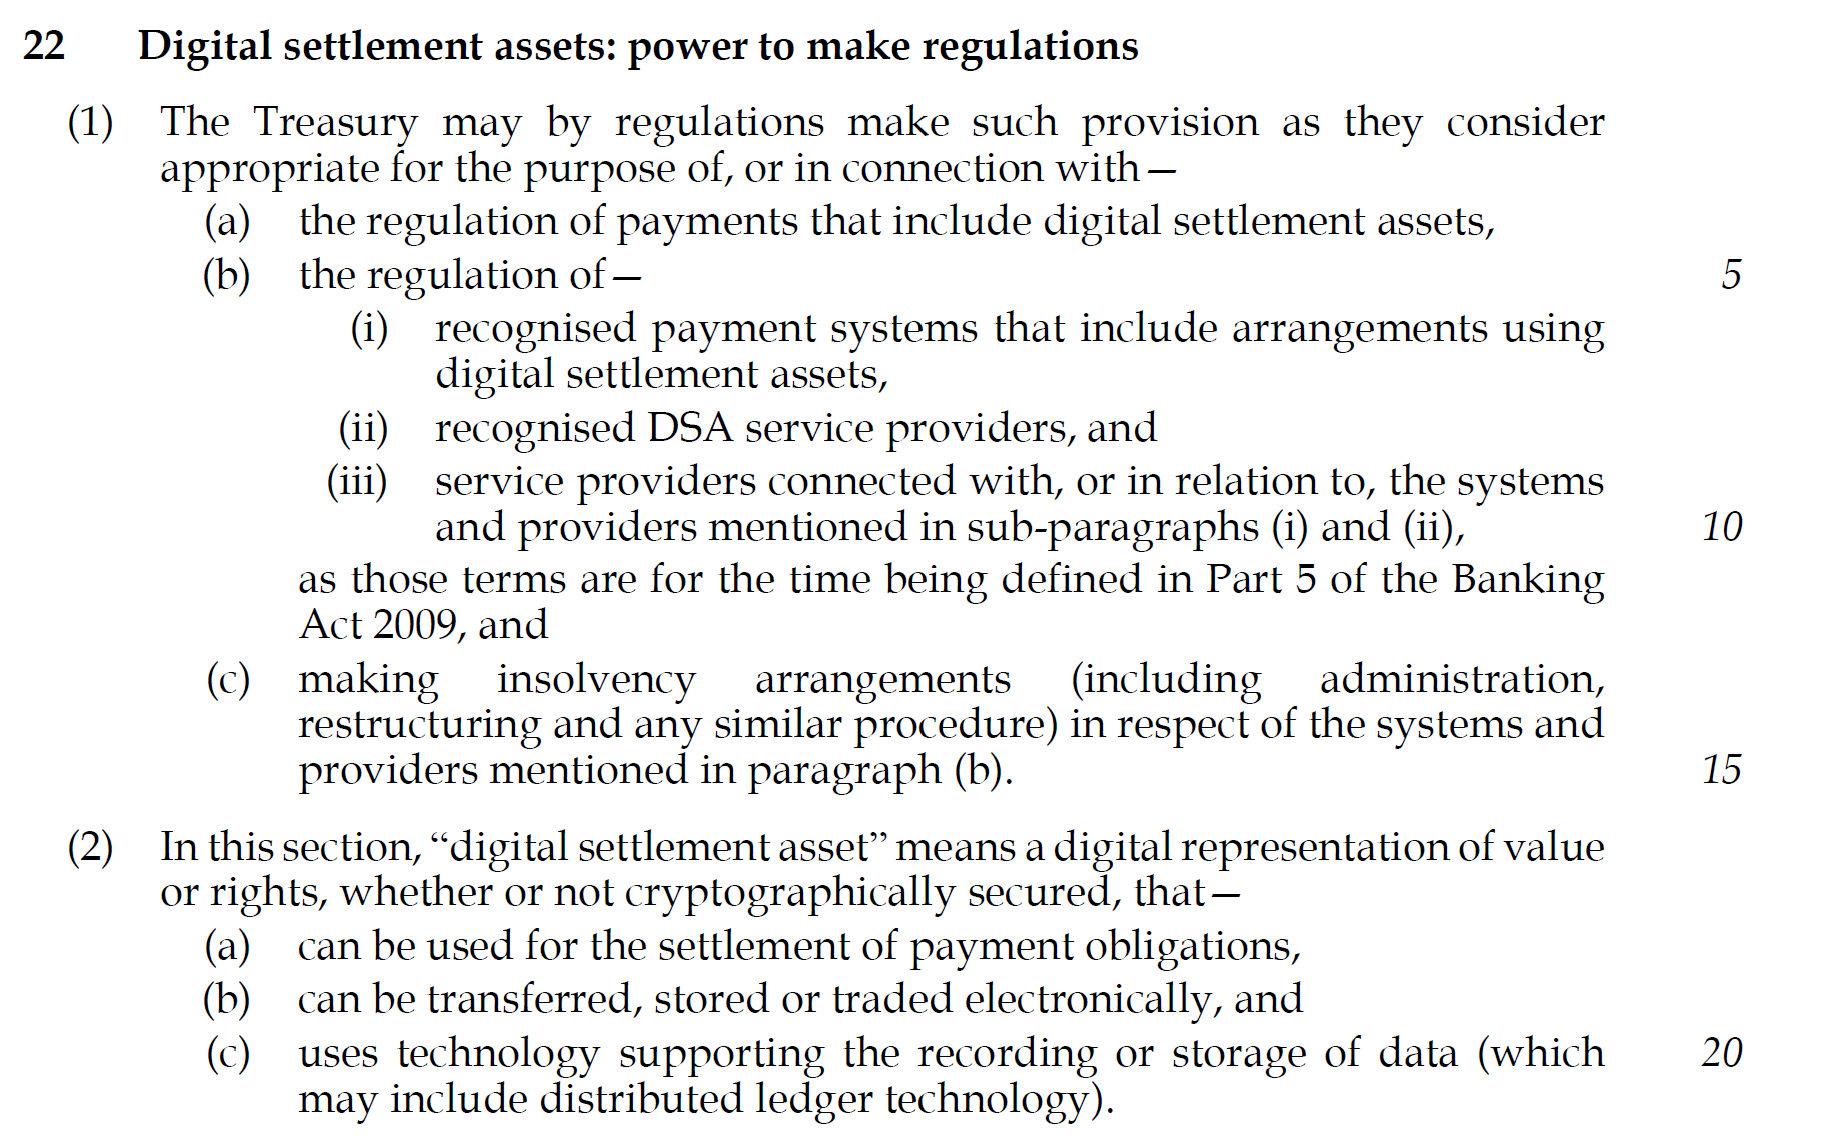
\includegraphics[width=\linewidth]{ukdigitalbill}
  \caption{The UK signs into law regulation of digital representatives of value}
  \label{fig:ukdigitalbill}
\end{figure}

\subsubsection{Stables in metaverse applications}
It makes a \textbf{lot} of sense to consider stablecoin transfer as the money in metaverses. USDC is furthest along this possible adoption curve. Their partnership with global payment provider Stripe has \href{https://stripe.com/blog/expanding-global-payouts-with-crypto}{enabled global dollar transfer} within Twitter for users of their `Connect' platform. This leverages the Polygon chain (mentioned in the blockchain chapter). Many digital wallets can be connected from the user end, with Metamask potentially being the easiest to integrate. This has also been mentioned in the book. The downside of this for our open platform is that none of these elements are particularly open, or distributed, and the users of the platform will still need to use an exchange to get the USDC to spend. This approach makes it easier for the vendors and product providers in the metaverse applications to accept USDC, but everything else is actually harder.

\section{Central bank digital currencies}
If 2022 was the year of the stablecoin then 2023 is likely to be the year of the central bank digital currency (CBDC). CBDCs would likely not exist without the 2019 catalyst of \href{https://www.thetimes.co.uk/article/facebooks-libra-cryptocurrency-project-ends-in-failure-cxvnnc3kx}{Facebook Libre} crypto currency project, which is now \href{https://fortune.com/2022/07/01/meta-novi-crypto-payments-wallet-end-september-2022/}{cancelled} and defunct, \href{https://www.theguardian.com/world/2021/jul/09/currency-and-control-why-china-wants-to-undermine-bitcoin}{pressure exerted on central banks} by the concept of Bitcoin, and the stablecoins which emerged from the technology.\par
It now seems plausible that the world is moving toward a plurality of national and private digital currencies. Figure \ref{fig:CBDClikely} from the Bank for International Settlement, shows the growing acceptance within central banks. Their 2022 annual economic report dedicates \href{https://www.bis.org/publ/arpdf/ar2022e3.pdf}{a 42 page chapter} to the subject. Hyun Song Shin, head of research at BIS said \textit{``Our broad conclusion is captured in the motto, ‘Anything that crypto can do, CBDCs can do better.``}\par
This text from the \href{https://voxeu.org/article/benefits-central-bank-digital-currency}{thinktank VoxEU} highlights the pressure on not to be \href{https://himes.house.gov/u-s-central-bank-digital-currency}{`left behind'}: \textit{``Given the rapid pace of innovations in payments technology and the proliferation of virtual currencies such as bitcoin and ethereum, it might not be prudent for central banks to be passive in their approach to CBDC. If the central bank does not produce any form of digital currency, there is a risk that it loses monetary control, with greater potential for severe economic downturns. With this in mind, central banks are moving expeditiously when they consider the adoption of CBDC.''} The Atlantic Council \href{https://www.atlanticcouncil.org/cbdctracker/}{have a website} which tracks global adoption.\par\par
\begin{figure}
  \centering
    \includegraphics[width=\linewidth]{CBDClikely}
  \caption{More than half of central banks \href{https://www.bis.org/publ/bppdf/bispap125.htm}{surveyed by the BIS} said they saw issuance of a CBDC as possible.}
  \label{fig:CBDClikely}
\end{figure}
CBDCs are wholly digital representations of national currencies, and as such are centralised database entries, endorsed and potentially issued by national governments. The \href{https://www.federalreserve.gov/publications/files/money-and-payments-20220120.pdf}{USA's whitepaper} shows the approach. Curiously only \href{https://www.sanddollar.bs/about}{The Bahamas} seem to have a successful implementation, but it is a rapidly evolving space, and many nations are now scrambling to \href{https://twitter.com/GobiernoMX/status/1476376240873517061}{catch up}. A \href{https://www.linkedin.com/feed/update/urn:li:activity:6980330210030145536/}{post on the LinkedIn page} of the Bank of International Settlements highlights a research project between 20 Asian banks which settles tens of millions of dollars using CBDC tooling.\par
The following text is taken from the March 2021 Biden government ``executive order'' on digital assets, and defines the current global legislative position well.\\
\textit{``Sec. 4.  Policy and Actions Related to United States Central Bank Digital Currencies.  (a)  The policy of my Administration on a United States CBDC is as follows:\\
(i) Sovereign money is at the core of a well-functioning financial system, macroeconomic stabilization policies, and economic growth.  My Administration places the highest urgency on research and development efforts into the potential design and deployment options of a United States CBDC.  These efforts should include assessments of possible benefits and risks for consumers, investors, and businesses; financial stability and systemic risk; payment systems; national security; the ability to exercise human rights; financial inclusion and equity; and the actions required to launch a United States CBDC if doing so is deemed to be in the national interest.\\
(ii)   My Administration sees merit in showcasing United States leadership and participation in international fora related to CBDCs and in multi‑country conversations and pilot projects involving CBDCs.  Any future dollar payment system should be designed in a way that is consistent with United States priorities (as outlined in section 4(a)(i) of this order) and democratic values, including privacy protections, and that ensures the global financial system has appropriate transparency, connectivity, and platform and architecture interoperability or transferability, as appropriate.\\
(iii)  A United States CBDC may have the potential to support efficient and low-cost transactions, particularly for cross‑border funds transfers and payments, and to foster greater access to the financial system, with fewer of the risks posed by private sector-administered digital assets.  A United States CBDC that is interoperable with CBDCs issued by other monetary authorities could facilitate faster and lower-cost cross-border payments and potentially boost economic growth, support the continued centrality of the United States within the international financial system, and help to protect the unique role that the dollar plays in global finance.  There are also, however, potential risks and downsides to consider.  We should prioritize timely assessments of potential benefits and risks under various designs to ensure that the United States remains a leader in the international financial system.''}\par

In traditional nation state currencies the central banks \href{https://www.bankofengland.co.uk/markets/bank-of-england-market-operations-guide}{control the amount} of currency in circulation by issuing debt to private banks, which is then loaned out to individuals \cite{wang2021central}. The debt is `destroyed' on the balance sheet to remove currency through the reverse mechanism. They also facilitate government debt \cite{filardo2012central}, and work (theoretically) outside of political control to adjust interest rates, in order to manage growth and flows of money. \par
It is somewhat surprising that Powell, chair of the US Federal Reserve has \href{https://www.federalreserve.gov/newsevents/speech/powell20220617a.htm}{recently said} \textit{``Rapid changes are taking place in the global monetary system that may affect the international role of the dollar. A US central bank digital currency is being examined to help the US dollar's international standing.''}. This is a rapid evolution of the narrative, with implications. It seems unlikely that the world would sacrifice the traditional banking system in favour of centrally controlled money, but many things which cannot be done with traditional nation state money systems are possible with CBDCs, because they \href{https://voxeu.org/article/benefits-central-bank-digital-currency}{remove the middleman} of private banking between the end user and the policy makers. 
\begin{itemize}
\item Negative interest rates are possible, such that all of the money can lose purchasing power over time, and at a rate dictated by policy. This ``removal of the lower bound'' has been discussed by economists over the last couple of decades as interest rate mechanisms have waned in efficacy. It is not possible in the current system, and instead money must be added through \href{https://www.bankofengland.co.uk/monetary-policy/quantitative-easing}{quantitative easing}, which disproportionately benefits some though Cantillon effects \cite{cantillon1756essai, bordo1983some}.  
\item Ubiquitous basic income is possible in that money can be issued directly from government to all approved citizens, transferring spending power directly from the government to the people. This also implies efficiency savings for social support mechanisms.
\item Asset freezing and confiscation are trivial if CBDCs can replace paper cash money completely, as a bearer asset. Criminals and global `bad actors' could have their assets temporarily or permanently removed, centrally, by suspending the transferability of the digital tokens.
\item Targeted bailouts for vital institutions and industries are possible directly from central government policy makers. Currently private banks must be incentivised to make cheap loans available to sectors which require targeted assistance.
\item Financial surveillance of every user is possible. In this way a `panopticon of money' can be enacted, and spending rulesets can be applied. For instance, social support money might only be spendable on food, and child support only on goods and services to support childcare. This is a very dystopian set of ideas. Eswar Prasad says ``In authoritarian societies, central bank money in digital form could become an additional instrument of government control over citizens rather than just a convenient, safe, and stable medium of exchange\cite{prasad2021future}.'' This is possibly \href{https://twitter.com/WallStreetSilv/status/1581378124452753408}{already happening} in China through integration of outstanding debt data with the social credit system.  
\item It's a virtually cost free medium of exchange, since there is no physical instrument which must be shipped, guarded, counted, assayed, and securely destroyed.
\item The counterfeiting risk is significantly reduced because of secure cryptographic underpinnings rather than paper or plastic anti counterfeiting technologies.
\item Global reach and control is instantly possible for the issuer. This is a big problem especially for a reserve currency such as the dollar. Two thirds of \$100 bills are \href{https://www.federalreserve.gov/pubs/ifdp/2012/1058/default.htm}{thought to} reside outside of the USA.
\item System level quantitative easing and credit subsidies are made far simpler and less wasteful when centrally dictated.
\item Transfer of liability and risk to the holder globally reduces the management costs for global deposits of a currency. 
\item It may be possible to automate the stability of a currency through continuous adjustment of the `peg' through algorithms or AI.
\end{itemize}

The UK has signalled that it is not interested in developing a CBDC at this time. It is viewed as a \href{https://committees.parliament.uk/publications/8443/documents/85604/default/}{solution in search of a problem}, with the Lords economic affairs committee saying:\textit{``The introduction of a UK CBDC would have far-reaching consequences for households, businesses, and the monetary system for decades to come and may pose significant risks depending on how it is designed. These risks include state surveillance of people’s spending choices, financial instability as people convert bank deposits to CBDC during periods of economic stress, an increase in central bank power without sufficient scrutiny, and the creation of a centralised point of failure that would be a target for hostile nation state or criminal actors.''}\par
Meanwhile in Europe, ECB President \href{https://www.ecb.europa.eu/press/pressconf/2022/html/ecb.is220310~1bc8c1b1ca.en.html#qa}{Christine Legarde} said: \textit{``On your question concerning CBDC, you know my views on CBDC and you know that I have pushed that project. Fabio Panetta is working hard on that together with members in the entire Eurosystem with the high-level taskforce that is working really hard on moving forward. But in a way, I am really pleased that attention is now focussed on the role that cryptos can play and the role that Central Bank Digital Currency can have when they are implemented. We have a schedule, as you know. The Governing Council decided back in October '21 to launch a two-year investigation phase, and it is at the end of that investigation phase that the decision will definitely be made to launch the CBDCs and to make it a reality. We can't go wrong with that project. I am confident that we will move ahead, but that's going to be a decision of the Governing Council. I think it's an imperative to respond to what the Europeans expect, and I think we have to be a little bit ahead of the curve if we can on that front. If we can accelerate the work, I hope we can accelerate the work. I will certainly support that and I was delighted to see that in the United States there was an executive order by President Biden to actually expect similar effort and focus and progress on CBDC, cryptos. I think that it will take all the goodwill of those who want to support sovereignty, who want to make sure that monetary policy can be transmitted properly using our currency, will endeavour.''}\par
India has expressed far more interest in the technology, and of course their addressable market is huge! They have published a  `\href{https://twitter.com/RBI/status/1578329048446828544?}{concept note}' in which they assert that a digital Rupee would be faster, cheaper, and easier to maintain. The key difference in India's situation is the large areas of the rural population where mobile internet is more patchy. In such situations a cash equivalent stablecoin token with cash finality which can be transferred between mobile phone wallets \textit{without} an internet connection is a huge boon. It seems very likely that India is moving to react to the innovation threat posed by cryptocurrencies to their own cash infrastructure. They are moving toward a pilot programme.\par
In the USA this text from Congressman Tom Emmer shows how complex and interesting this debate is becoming.\textit{``Today, I introduced a bill prohibiting the Fed from issuing a central bank digital currency directly to individuals. Here’s why it matters: As other countries, like China, develop CBDCs that fundamentally omit the benefits and protections of cash, it is more important than ever to ensure the United States’ digital currency policy protects financial privacy, maintains the dollar’s dominance, and cultivates innovation.\\
CBDCs that fail to adhere to these three basic principles could enable an entity like the Federal Reserve to mobilize itself into a retail bank, collect personally identifiable information on users, and track their transactions indefinitely.\\
Not only does this CBDC model raise ``single point of failure'' issues, leaving Americans’ financial information vulnerable to attack, but it could be used as a surveillance tool that Americans should never be forced to tolerate from their own government.\\
Requiring users to open an account at the Fed to access a United States CBDC would put the Fed on an insidious path akin to China’s digital authoritarianism.\\
Any CBDC implemented by the Fed must be open, permissionless, and private. This means that any digital dollar must be accessible to all, transact on a blockchain that is transparent to all, and maintain the privacy elements of cash.\\
In order to maintain the dollar’s status as the world’s reserve currency in a digital age, it is important that the United States lead with a posture that prioritizes innovation and does not aim to compete with the private sector.\\
Simply put, we must prioritize blockchain technology with American characteristics, rather than mimic China’s digital authoritarianism out of fear.''}\par
Most analysts now seem to think that there is little appetite to replace established 'Western' cash with CBDCs. Most significantly such products would need the support of retail banks, and it is not in their interest to service such a product. Their business model relies on using retail deposits for providing loans, and it is these deposits, not cash itself that would be the most addressable market for a CDBC. Banks don't want people to self custody money. In addition it exposes the whole banking system to a higher risk of bank runs. Such a self custody, interest bearing, central government backed asset would have significantly less counterparty risk than even bank deposits, and at times of high systemic stress it seems likely that money would flow to where it's thought safest, exposing the retail banks to runs. All of the proposed solutions to these problems such as caps and negative interest penalties seem poorly thought through.\par
It is far more likely that a blend of stablecoins, private bank issued digital currency (with a yield incentive) and perhaps some limited CBDC, alongside the new contender Bitcoin, will present a new landscape of user choice. Different models of trust, insurance, yields, acceptability, and potentially privacy, will emerge. \par
Clearly a global, stable, wholly digital bearer asset in a native currency would be the ideal integration for money in a metaverse application, but it is likely that a transition to such a technology would be complex and painful. It is certainly not ready for consideration now.
\section{Bitcoin as a money}
Nwosu, cofounder of Coinfloor exchange in the UK, and cofounder of the aforementioned Fedimint and says that a digital money needs the following four characteristics:
\begin{itemize}
\item that it be technically mature. %Nwosu does not see Ethereum as demonstrating this for instance due to it's change to proof of stake. This is the same reasoning outlined in the blockchain section of this book.
\item it should have strong community support and network effect. We have seen that this is more simply a feature of money itself.
\item that there should be regulatory clarity around the asset, a feature which even Bitcoin currently struggles with.
\item it should demonstrate a core use case of `store of value' which sounds simple enough, but again is contestable because of the volatility of Bitcoin.
\end{itemize}
\subsection{Spending it}
Since this book seeks to examine transfer of value within a purely digital environment it is necessary to ask the question of whether Bitcoin is money. This short \href{https://bitcoin-zar.blogspot.com/2018/07/duality-excerpt-by-satoshi-nakomoto.html}{`story'}, purportedly written by Nakamoto, is a fabulous look at the money values of the technology, irrespective if it's provenance. In it is the following text: \textit{``Here, for once, was this idea that you could generate your own form of money. That's the primary and sole reason, is because it was related to this thing called money. It wasn't about the proficiency of the code or the novelty, it was because it had to do with money. It centered around money. That is something people cared about. After all, plenty of projects on Sourceforge at the time were just as well coded, well maintained, if not better, by teams, and even if someone else had created the blockchain before me, had it been used for something else beyond currency, it probably would not have had much of an outcome.}\par
Again, irrespective of the author here, this point seems to ring true. The memetic power of Bitcoin is in it's proximity to `money', and the potential of the separation of money from the state. \par
It is beyond argument that the Bitcoin network is a rugged message passing protocol which achieves a high degree of consensus about the entries on it's distributed database.\par Ascribing monetary value to those database entries is a social consensus problem, and this itself is a contested topic. The most useful `hot take' here is that Bitcoin behaves most like \href{https://twitter.com/saylor/status/1395788419301773312}{a `property'}, while it's network behaves far more like a monetary network which is created and supported by the \href{https://saito.tech/an-response-to-paul-krugman-from-a-keynesian-bitcoiner/}{value of the Bitcoin tokens}. \par
Jack Mallers, of Strike \href{https://www.youtube.com/watch?v=jb-45m9f76I}{presentation to the IMF} identified the following challenges which he claims are solved by the bitcoin monetary network.
\begin{itemize}
\item Speed
\item Limited transparency and dependability
\item High cost
\item Lack of interoperability
\item Limited Coverage
\item Limited accessibility
\end{itemize}
He further identifies the attributes of the ideal global money. 
\begin{itemize}
\item Uncensorable
\item Unfreezable
\item Permissionless
\item Borderless
\item Liquid
\item Digital
\end{itemize}
Mallers has recently announced USA focused partnerships which leverage his Strike product to enable spending Bitcoin, through Lightning, as Dollars in much of the \href{https://www.ncr.com/point-of-sale-pos-systems}{point of sale} infrastructure in the USA. This is a huge advance as it immediately enables the vendors both online and at physical locations to either save 3\% costs for card processors, or else pass this on as a discount. Crucially for `Bitcoin as a money' it also allows the vendors to receive the payment \textbf{as} Bitcoin, not Dollars. A possible further and highly significant feature is that it might now be possible to divest of Bitcoin in the USA, buying goods, without a capital gains tax implication. Mallers claims to have legislative backing for this product, but the devil will likely be in the detail. The likely mechanism for this product is that the EPOS partner sends a Lighting request to Strike, which liquidates some of their Bitcoin holding to a dollar denominated stablecoin, but in a tax free jurisdiction such as El Salvador. This stablecoin will then be sent to the EPOS handing partner such as NCR. Stablecoin to Dollar transactions in the USA are much murkier and likely don't cost anything for these companies. This agent will then authorise the Dollar denominated sale to the American digital till. Crucially nobody has a US capital gains tax exposure in this chain, and all of the settlements were near free, and instantaneous, with `cash finality' for everyone except the EPOS company. They are likely actually exposed to a small risk here because uptake will be very low level. The novelty opportunity will likely cover any potential exposure to stablecoin collapse. This is a radical upgrade on the normal flow of divesting Bitcoin for American users. \par
Using this open product to spend Bitcoin as Bitcoin to vendors might be available through Shopify globally. Again, it's too new to be sure. Promisingly a \href{https://www2.deloitte.com/content/dam/Deloitte/us/Documents/technology/us-cons-merchant-getting-ready-for-crypto.pdf}{Deloitte study} has found that 93\% of businesses accepting Bitcoin have seen revenue and brand perception improve, and 75\% of USA sales execs plan to accept digital assets at some point in the next 2 years. This ambition in the US markets is likely to benefit from the proposed \$200 tax exempt law for purchasing goods and services with Bitcoin.\par
Of these recent developments in Lightning \href{https://twitter.com/LynAldenContact/status/1512188883101966351}{Lyn Alden says}: \textit{Some people naturally dismiss [strike] because they don't want to spend their BTC; they want to save it. However, the more places that accepted BTC at point of sale (on-chain or Lightning or otherwise), the more permissionless the whole network is. This is because, if all you can do with BTC is convert it back into fiat on a major exchange, then it's easy to isolate it, effectively blacklist addresses, etc. But if you can directly spend it on goods and services across companies and jurisdictions, it's harder to isolate. There are now plenty of vendors that make this easy for merchants to implement, and the merchant can still receive dollars if they want (rather than BTC), or can decide their \% split. Since it's an open network, anyone can build on it, globally. And then when you add fiat-to-BTC-to-fiat payments over Lightning, it gets even more interesting because it doesn't necessarily need to be a taxable event. Lightning wallets with a BTC balance and a USD/stablecoin balance. Lower fees than Visa and others.}\par
\subsubsection{Bitcoin based FIAT}
More interestingly for metaverse applications Mallers has opened this section of the company to interact with the public Lightning network, allowing people with a self hosted wallet or node to pay directly for goods across America, settling immediately in Dollars, using their Bitcoin, at zero cost. \textbf{This opens the possibility to buy from US based (Dollar denominated) metaverse stores, using the capabilities of the stack assembled at the end of the book}. The implications globally are unclear at this time.\par
\href{https://stablesats.com/}{Stablesats} is another approach which uses exclusively lightning bitcoin but makes the value stable against the US dollar using an algorithm. This is a very interesting option and will be explored in detail at some point.
\subsection{Saving with it} 
The Bitcoin community believes that \href{https://svetski.medium.com/why-bitcoin-not-shitcoin-6cc826f4fa52}{Bitcoin is the ultimate money}, a \href{https://www.coindesk.com/business/2022/01/07/jpmorgan-sees-more-crypto-adoption-in-2022-debates-bitcoins-status-as-store-of-value/}{`store of value'}, chance to \href{https://www.forbes.com/sites/leeorshimron/2020/06/30/bitcoin-is-the-separation-of-money-and-state/?sh=49294a8356db}{separate money from state}, increase \href{https://www.washingtonpost.com/national/locked-out-of-traditional-financial-industry-more-people-of-color-are-turning-to-cryptocurrency/2021/12/01/a21df3fa-37fe-11ec-9bc4-86107e7b0ab1_story.html}{equality of opportunity} and \href{https://iai.tv/articles/the-rich-get-richer-the-poor-get-bitcoin-auid-1766}{ubiquity of access}, while others view it as \href{https://www.cnbc.com/2021/06/22/a-third-of-investors-think-bitcoin-is-rat-poison-jpmorgan-survey-says.html}{`rat poison'}, or a \href{https://jacobinmag.com/2022/01/cryptocurrency-scam-blockchain-bitcoin-economy-decentralization}{fraudulent Ponzi scheme} \cite{ponzi2021alden}. A notable exclusion from the negative rhetoric is Fidelity, the global investment manager, who have always been positive and have \href{https://www.fidelitydigitalassets.com/articles/bitcoin-first?sf253214177=1}{recently said}: 
\textit{``Bitcoin is best understood as a monetary good, and one of the primary investment theses for bitcoin is as the store of value asset in an increasingly digital world.''}\par
The following paraphrases Eric Yakes, author of \href{https://yakes.io/book/}{`The 7th Property'}. Again, this is an Austrian economics perspective, and like much economic theory the underlying premise \href{https://medium.datadriveninvestor.com/do-you-understand-the-austrian-vs-keynesian-economic-debate-2f4b152c6a6b}{is contested}\cite{maurel2012keynesian}: \textit{``Paper became money because it was superior to gold in terms of divisibility and portability BUT it lacked scarcity. People reasoned that we could benefit from the greater divisibility/portability of paper money as long as it was redeemable in a form of money that was scarce. This is when money needed to be ``backed'' by something. \\
Since we changed money to paper money that wasn't scarce, it needed to be backed by something that was. Since the repeal of the gold standard, politicians have retarded the meaning of the word because our money is no longer backed by something scarce.\\
So, what is bitcoin backed by? Nothing.\\
Sound money, like gold, isn’t ``backed''.
Only money that lacks inherent monetary properties must be backed by another money that maintains those properties. The idea that our base layer money needs to be backed by something is thinking from the era of paper money. Bitcoin does not require backing, it has inherent monetary properties superior to any other form of money that has ever existed.''}\par
The 2022 ARK Big Ideas report again provides some useful market insight. They posit that demand for the money features of Bitcoin could drive the price of the capped supply tokens to around 1M pounds per Bitcoin as in Figure \ref{fig:BitcoinShareOfMoney}. Take this with the usual pinch of salt, as Ark have been performing notably badly lately with their predictions.
\begin{figure}
  \centering
    \includegraphics[width=\linewidth]{BitcoinShareOfMoney}
  \caption{Potential market exposure to Bitcoin as a money}
  \label{fig:BitcoinShareOfMoney}
\end{figure}
Perhaps more than any of these takes, it is worth considering the current public perception of the technology as a money and store of value. This \href{https://twitter.com/saquon/status/1480738426236375041}{twitter thread} from professional sportsman Saquon Barkley, to his half million followers on the platform, captures the mood. He is one of a handful of athletes now being \href{https://www.buybitcoinworldwide.com/athletes/}{paid directly} in Bitcoin.\par
\textit{``I want my career earnings to last generations. The average NFL career is 3 years and inflation is real. Saving and preserving money over time is hard, no matter who you are.
In today’s world: How do we save? This is why I believe in bitcoin. Almost all professional athletes make the majority of their career earnings in their 20s. With a lack of education, inaccessible tools, and inflation, a sad yet common reality is many enter bankruptcy later on. We can do better. We need to improve financial literacy. Bitcoin is a proven, safe, global, and open system that allows anyone to save money. It is the most accessible asset we’ve ever seen.''}\par
This ubiquity of access is what probably most distinguishes Bitcoin. Previously it could be argued that only the most wealthy could access the `means' to store their labour without loss of value over time (through inflation). To be clear, inflation is an important part of the money system, somewhat within the control of the central banks, and approximate to taxation. It applies equally to all holders of the money supply. Asserting that money should be replaced by a `hard asset' such as Bitcoin, in the place of the more controllable utility of money, is likely both a fantasy, and wrong minded. This conflation of money and property is a confusion caused by Bitcoin's proximity to money, and it's `money like' network, and is extremely commonplace.\par
These narrative takes are all rooted in the popular idea that Bitcoin is a `hedge against inflation'; an increasingly fragile take, as the price plummets with global markets. The Bitcoin community seems somewhat confused about the nature of money, which is predictable because we can see in these sections that money is pretty confusing. Money is the fluid, elastic \cite{cagan1958demand}, and thin `working credit' layer on top of historical human production, which provides transaction convenience, and tools for credit. Value is effectively swapped in and out of this layer through the actions of central banks, controlling inflation into acceptable margins. Simplistically this is done through manipulation of interest rates (the easiness of credit), quantitative easing (buying of assets) and quantitative tightening (selling of assets). It is primarily \textit{not} a long term store of value, as Austrian economists perhaps believe it should be. This function is left to assets. The Austrian thesis of `hard money' (which cannot be `debased' by government action) seems somewhat naive when one considers that if credit exists anywhere in the world (ie, the creation of paper money through loans) then this would be used to buy up a hard money asset in the long run, causing a scarcity crisis. This is what happened to gold in the middle of the last century. \par 
Fundamentally, Bitcoin isn't money (in the traditional sense) because it's not an IOU, which money certainly is. It's a bearer instrument, novel asset class, with money like properties, as identified above. As said again and again it functions most like a `property' which can be invested in by anyone, with all the attendant risks of that property class to the holder. Lyn Alden says it sits \href{https://www.lynalden.com/what-is-money/}{somewhere between} a saving tool, and an investment, acting as ``programmable commodity money''.\par 
\href{https://andrewmbailey.com/}{Andrew M. Bailey} says \textit{``in an ideal world where governments honour the rights of citizens, they don't spy, they don't prohibit transactions, they manage a sound money supply, and they make sound decisions, the value of bitcoin is very low; we're just not in an ideal world''}\par
Another potentially important differentiating affordance is censorship resistance. There's really nothing else like it for that one feature. With that said Bitcoin is only a viable `money like thing' when viewed in the layers described in this book, \href{https://giacomozucco.com/layers-before-bitcoin}{and elsewhere}\cite{Bhatia2021}. The base chain layer is an apex secure store of value. Whatever layer 2 ultimately emerges is the transactional layer which could replace day to day cash money, while the hypothetical layer 3 might be useful for complex financial mechanisms and contracts operating automatically, and also provides the opportunity for using the security model of the chain to support other digital assets, including government currencies through stablecoins. All these things have a natural home in borderless social spaces.
\section{Risks (money, not technical)}
Special thanks to economist Tim Millar for help with this section.
\subsection{Risks to Bitcoin the money}
\subsubsection{Geopolitics}
It can be seen that following the invasion of Ukraine by Russia, that sanctions of various kinds were applied to the Russian economy. One of these was the previously dicussed Swift international settlement network. Another whole catagory was the removal of support by private businesses domiciled outside of Russia and Ukraine, and pertinent here is that VISA, Mastercard, Paypal, and Western Union all removed support for their product rails. This means that while some cards and services still work, and will likely work again through Chinese proxies in the coming months, considerable disruption will be felt by Russian companies and individuals. This is not to say that this disruption is necessarily wrong, but it is clear now that all of these global financial transfer products and services are contingent on political factors. The same might be true of CBDC products if they gain traction globally. There is certainly no reason why all money within a physically delineated border could not be blocked or cancelled. This is not as true for Bitcoin at this time. \par 
However, with enough political will it is technically plausible to incentivise miners with additional payments to exclude transactions from geolocated wallets. This would be mitigated by Tor, and in a global anonymous network it is very likely that a miner could be found at a higher price for inclusion in the next block. \par
We have already seen much negative political positioning related to the energy concerns in an earlier chapter. There are similar noises coming from policy makers with regard to the money utility of the technology. The United Nations \href{https://unctad.org/system/files/official-document/presspb2022d8_en.pdf}{have made the following recommendations}:
\textit{``Developing countries may have less room to manoeuvre, yet the regulation of cryptocurrencies is possible. The following policies, among others, have the potential to curb the further spread of the risks of cryptocurrencies and stablecoins:
\begin{itemize}
\item Ensuring comprehensive financial regulation, through the following actions:
\begin{itemize}
\item Require the mandatory registration of crypto-exchanges and digital wallets and make the use of cryptocurrencies less attractive, for example by charging entry fees for crypto-exchanges and digital wallets and/or imposing financial transaction taxes on cryptocurrency trading;
\item Ban regulated financial institutions from holding stablecoins and cryptocurrencies or offering related products to clients;
\item Regulate decentralized finance (such finance may, in fact, not be fully decentralized, given its central management and ownership, which form an entry point for regulation);
\end{itemize}
\item Restricting or prohibiting the advertisement of crypto-exchanges and digital wallets in public spaces and on social media. This new type of virtual, and often disguised, advertisement requires policymakers to expand the scope of regulation beyond traditional media. This is an urgent need in terms of consumer protection in countries with low levels of financial literacy, as even limited exposure to cryptocurrencies may lead to significant losses;
\item Creating a public payment system to serve as a public good, such as a central bank digital currency. In the light of the regulatory and technological complexity of central bank digital currencies and the urgent need to provide safe, reliable and affordable payment systems, authorities could also examine other possibilities, including fast retail payment systems.
\end{itemize}
}
This is tough talk. We have seen that the IMF is willing to make their loans contingent on such regulation. This global response to the technology is a significant headwind, but like the internet itself, it's very hard to actually stop these products being used.
\subsubsection{Liquidity Lottery}
Because holders of BTC are disincentived to sell the asset (assuming future gains) it is likely vulnerable to something \href{https://twitter.com/UrbanKaoboy/status/1526311908709502977}{Kao called the `liquidity lottery'}. This is a supply/demand mismatch which he thinks could spell the end of the asset class in time. 
\subsubsection{Manipulation of price or the network}
Bitcoin is still young and illiquid enough to be highly manipulable. Imagine for instance if a major organisation or nation state wished to accumulate a significant amount of the asset, but would prefer a lower price. \par%To pick a mechanism at random, they could force a de-pegging of UST in the Terra/Luna ecosystem, forcing the algorithmic selling of Do Kwon's multi-billion dollar Bitcoin reserve contingency. This would immediately crash the price. 
There is an unknown level of exposure to risk from centralised mining. If a few of the major mining pools were simultaneously infiltrated by a nation state actor then it might be possible to engineer a `deep re-org' of a large transaction. This would be dealt with quickly and almost certainly be a transient attack, but the damage to the narrative might be substantial. A similar vulnerability exists in the centralisation at the level of internet service providers \cite{apostolaki2017hijacking}. This or some other flaw might lead to a selling cascade. Nobody knows just how vulnerable to selling cascades Bitcoin might be against a really serious challenge by an empowered actor, but it's already high volatility is suggestive of risk. 
\subsubsection{Rehypothecation}
It's vulnerable to rehypothecation (paper bitcoin managed by centralised entities running a fractional reserve). It seems that Figure \ref{fig:talebturkey} by  Nassim Taleb is a cautionary tale \cite{taleb2012antifragile}.
\begin{figure}
  \centering
    \includegraphics[width=0.7\linewidth]{talebturkey}
  \caption{Nassim Taleb's Turkey Problem}
  \label{fig:talebturkey}
\end{figure}
\subsubsection{Scale}
Scalability is always going to be a problem for Bitcoin, for all the reasons discussed in the blockchain chapter. There is no ``ready to go'' solution (except perhaps federations) that could onboard the whole world at this time because of the limited number of available UTXOs.\par 
Finally, a lack of fungibility, and privacy by default in Bitcoin, trends towards blacklists and over time this could seriously compromise the use of the asset. 
\subsubsection{Centralisation of the money over time}
In a medium term future it's possible to imagine a smart enough autonomous AI or ML actor managing to accrue Bitcoin through fast and smart `decisions'. This could unreasonably centralise the asset, and it would be impossible to claw this situation back. These constructs would last for the lifetime of the chain unless constrained by timelock multisigs for instance. 
\subsection{Bitcoin externalities}
This section is the risks that Bitcoin poses to external money systems, but it's worth pointing out that a risk to wider society is clearly \textit{also} a risk to Bitcoin itself.
\subsubsection{Inherent volatility}
One of the better public analysts of the asset, \href{https://twitter.com/davthewave/status/1072441941390974982/photo/1}{sees the price} eventually fluctuating somewhere between ~\$700k and ~\$300k.  Figure \ref{fig:davethewave}. This is not how a money is supposed to work.  

\begin{figure}
  \centering
    \includegraphics[width=\linewidth]{davethewave}
  \caption{\href{https://davethewave.substack.com/p/cycle-theory-revisited?s=r}{Cycle theory revisited blog post} [Image used with permission]}
  \label{fig:davethewave}
\end{figure}

Neither though is it the endless \href{https://stephanlivera.com/episode/147/}{``number go up''} that speculators have been promised. The aims of the project have a cognitive dissonance right at the core. The volatility trends toward:
\subsubsection{Unfair distribution}
By design the distribution of Bitcoin is likely `fair`, in that everyone has been able to access and secure the asset long term without prejudice. Figure \ref{fig:btcdistribution} from Twitter user @Geertjancap shows the distribution in 2021. Whether this is judged to be fair if the asset jumps to 10 times it's current value, minting a new class of hyper rich holders, is another matter. 
\begin{figure}
  \centering
    \includegraphics[width=\linewidth]{btcdistribution}
  \caption{\href{https://twitter.com/Geertjancap/status/1380972132990136322/photo/1}{Bitcoin distribution is skewed to s few early holders, but it likely \textbf{is} fair.} [Image used with permission]}
  \label{fig:btcdistribution}
\end{figure}
This pressure to emulate the early winners leads to:
\subsubsection{Endless HODL}
It's possible that there's a problem with people not wanting to sell the asset, because they are predisposed to a particular fervour promoted within the community. This can be seen in the \href{https://en.macromicro.me/charts/32355/bitcoin-supply-last-active-1plus-years-ago}{glassnode data}, where the black line in Figure \ref{fig:notselling} shows that the asset held for more than a year (illiquid) has increased over the years.
\begin{figure}
  \centering
    \includegraphics[width=0.5\linewidth]{notselling}
  \caption{Supply of bitcoin that \href{https://en.macromicro.me/charts/32355/bitcoin-supply-last-active-1plus-years-ago}{hasn't moved} for over 1 year}
  \label{fig:notselling}
\end{figure}
There's real recalcitrance about using the asset as a money, which leads to:
\subsubsection{Reduction of funding source / liquidity in legacy finance}
In the current financial system remuneration for labour performed in the workforce is loaned into the money system, where it's put to work providing liquidity for creation of more opportunity. This system actually works pretty well. The more of this deferred labour that's taken out of the legacy system, the less work can be done with what remains. This isn't to say that Bitcoin will cause a liquidity crisis, but there is possibly a cost if the current trend continues. This isn't as bad as:
\subsubsection{Bitcoin collapse system shock}
In the event of an existential collapse of the Bitcoin network the erasure of so much capital would certainly have a contagion effect on the whole global financial system. It's hard to imagine what such an event could be, this being the nature of ``black swans''. One cited example is the unravelling of cryptography by quantum computing. Some conspiracy theorists in the past have even speculated that Bitcoin is itself a canary in the coal mine, engineered by the NSA to warn about emergent quantum computing somewhere in the world. It's all pretty silly because without cryptography Bitcoin would be the least of humanities problems. The risk of `something' does exist though. The same anti-fragile feature can't be said about the technologies around Bitcoin, which gives us:
\subsubsection{Stablecoin collapse system shock}
This is much more likely. Stablecoins are under regulated, centralised, under collateralised, ponzo like structures, which could quite clearly fall apart at any point. The contagion effects of this are unclear as they're not yet too significant. They're a risk nontheless, and may be an indicator of:
\subsubsection{Tech for techs sake yielding unexpected outcomes}
The whole question of what Bitcoin addresses, whether it's been properly thought about, what the end goals are, and what the risks are is significant. It's a computer science and engineering solutions gone completely wild. It's clearly got benefits and there's clearly human appetite for this technology, but it's probably running ahead of the knowledge base around it. This is most exemplified in:
\subsubsection{No agreed measurable end goal}
 Bitcoin is a game theoretic juggernaut, where success of the network breeds more success for the network. The was obviously a great design choice for the computer scientists trying to solve the problem of a secure, and scalable, electronic cash, which couldn't be confiscated. Ironically for a global consensus mechanism it seems that nobody wants to discuss what constitutes a successful end point to this, and especially not what `successful' endpoints for the game theory which have calamitous negative repercussions for wider society look like.  This might have implications for:
\subsubsection{National security / actual warfare}
There's some national security implications for Bitcoin which are discussed both in the \href{https://twitter.com/JasonPLowery/status/1512775981693648897?}{fringes} and the \href{https://www.coindesk.com/layer2/2022/04/04/why-bitcoin-mining-is-a-matter-of-national-security/}{sector media}. Essentially, the industrial mining complexes which are more commonplace now, are easily identifiable targets, and provide nations with both some leverage over the global network, and a considerable source of income. The IMF correctly identifies these facilities as a way for nation states to \href{https://www.imf.org/en/Publications/GFSR/Issues/2022/04/19/global-financial-stability-report-april-2022}{monetise their energy reserves} without the need for foreign markets, opening the door to sanction avoidance. In the case of smaller and developing nation states who are perhaps subject to financial penalties on the global stage for whatever reason, these facilities start to look like legitimate targets for cyber and conventional warfare. This `weaponisation' of a neutral technology is already manifest in:
\subsubsection{Bitcoin as a culture war foil}
Bitcoin's online community skews very hard toward right wing libertarianism. This isn't to say there are no other voices, but they are certainly outnumbered. This imbalance is almost certainly a product of the ESG concerns around the technology. There has been a notable increase in diversity of thought since the evolution of the energy narrative, but it persists. This leads to a paucity of voices in policy making circles, and in the USA a strong delineation between policy makers along party lines. This kind of thing tends to be self reinforcing, and it seems very possible that the global liberal left will swing mainly against the technology, while the neoliberal right will be attracted more to it. As tensions increase so it seems does the online rhetoric. Even scientists now seem to agree that Bitcoin investors are calculating psychopaths \cite{martin2022dark}. This leads to:
\subsubsection{Self reinforcing monocultures}
There are some powerful `pockets' of fringe thinking within the \href{https://pourteaux.substack.com/p/bitcoin-culture-burn-it-to-the-ground?}{vocal, online, Bitcoin communities}. The \href{https://www.forbes.com/sites/peterizzo/2022/07/04/bitcoin-maximalism-is-dead-long-live-bitcoin-maximalism/?}{most palatable} of these are figures like \href{https://www.saylor.org/about/}{Michael Saylor}, Elon Musk and Jack Dorsey, but there's whole subcultural intersections around antivax, anti-woke, anti cancel culture, and fad diets. It might seem that this isn't terribly important, but Bitcoin viewed though the lens of these of these communities looks pretty strange to the newcomer. The early adopters are just using their wealth to leave the battlefield behind using:
\subsubsection{Jurisdictional / legislative  arbitrage}
The reach of Bitcoin and it's ability to undercut the global money systems, delivering savings for those with a first mover advantage, and the current paucity of agreed legislation has set up an interesting and rare condition. Bitcoin encourages something called jurisdictional arbitrage; the race to take advantage of the variance in national approaches to the asset class. This section could perhaps be explored as a list of opportunities, but from the viewpoint of our SME business use case it's far more likely that these destabilising `features' are risks: 
\begin{itemize}
\item \textbf{Difference in `crypto' profit models}. Countries and jurisdictions can apply different charges for use of trading platforms and capital gains tax enjoys huge variance. Some countries are now competing to offer zero tax as a way to attract valuable tech mind share. 
\item \textbf{Income tax} is harder to monitor in a truly international context. This is variously pitched around the world.  It's hard to monitor this stuff and tax at source like with company employees wages, because it's basically designed to be hard to monitor. This results in:
\item \textbf{Passport perks}. Countries are already selling residence and company rights against Bitcoin marketing. There's a lot of new ways to buy passports and citizenship based on `inclusion' in this community now. It's a terrible look. The early adopters can live international jetsetter lifestyles and ca benefit from:
\item \textbf{Business subsidies} such as those appearing in Switzerland, \href{https://davisclute.medium.com/visiting-a-startup-city-in-honduras-73d9c026ee6d}{Hondoras}, El Salvador, Africa etc. This means a new divide is emerging since some countries are in instead applying:
\item \textbf{KYC/AML} rules which make onboarding into this technology harder. Currently there's a trend toward globally capturing information about people buying these assets, but it's effectively tech warfare now with engineers, rapidly producing tools to circumvent slow and varied legislation. The best example of this remains El Salvador, where Bitcoin is legal tender, and has perhaps kickstarted:
\item \textbf{Bond issuances}. El Salvador are having a \href{https://www.ft.com/content/4fa63c8c-51f5-4512-b522-76dd75e62916}{faltering start} to their promised bond issuance. It might be that all of this is a harbinger of the rise of: 
\item \textbf{The Network State} is a proposal by Srinivasan \cite{Srinivasan2022}. His is a transhumanist thesis which he describes: \textit{``The fundamental concept behind the network state is to assemble a digital community and organize it to crowdfund physical territory. But that territory is not in one place — it’s spread around the world, fully decentralized, hooked together by the internet for a common cause, much like Google’s offices or Bitcoin’s miners. And because every citizen has opted in, it’s a model for 100\% democracy rather than the minimum threshold of consent modeled by 51\% democracies.''}
%\href{https://prospera.hn/news/press-releases/pr\%C3\%B3spera-announces-bitcoin-bond-authority-in-the-first-crypto-friendly-jurisdiction-that-is-fully-aml-kyc-compliant}{Prospera}\\
\end{itemize}
\subsubsection{Hyperbitcoinization}
All of the above starts to look like convergence on something the crypto community regularly describes to itself within it's internal media. Hyperbitcoinization is a term coined in 2014 by Daniel Krawisz \cite{krawisz2014hyperbitcoinization}. It is the hypothetical rise of Bitcoin to become the global reserve currency, and the demonetisation of all other store of value assets. This seems unlikely but is hinted at in a game theoretic analysis of both Bitcoin and current macro economics. Again, Bitcoin is a likely very poor replacement for money. The ability to monetise assets through banks, backed by law and contracts (the debt based system), is a highly refined human concept, while Bitcoin is a fusion of Austrian economics, and a computer science project. The hyperbitcoinization idea finds it's ultimate expression in Svalholm's ``Everything Divided by 21 Million'', a hypothetical re-accounting of all human production into the Bitcoin ledger \cite{booth2022bitcoin}.\par
Nobody is sure what a \href{https://fredblog.stlouisfed.org/2022/07/inflation-and-deflation-with-a-fixed-money-supply/}{regular deflationary cycle} might do to global supply chains. Malherbe et al. point out the inherent unsuitability of a deflationary asset such as Bitcoin as the global reserve currency \cite{malherbe2019cryptocurrencies} and feel that perhaps other cryptocurrencies might be more suitable for adoption by governments.  Interestingly this is the only paper to reference `Duality' (the only thing purportedly written by Satoshi Nakamoto after they left the project). \par
Writer and activist Cory Doctorow is \href{https://onezero.medium.com/the-byzantine-premium-8411521db843}{not a fan of Bitcoin}. He provides an excellent summary of what he sees as the \href{https://doctorow.medium.com/finance-caused-the-fall-of-rome-fd091fa02973}{basic societal mistake} of the libertarian ideals around strong property rights and hard money. In a hyperbitcoinised world where debt law would be enforced by distributed code, it might be far harder to prevent the ``fall of Rome'' scenario he describes.  \par  
Fulgur Ventures (a venture capital firm) provide a \href{https://medium.com/@fulgur.ventures/the-roads-to-hyperbitcoinization-part-1-27dc84d0e5e5}{blog post series} about the route this might take. It's important to note that Budish suggested that the usefulness of Bitcoin (and blockchain) cannot exceed the cost to attack it. The is highly suggestive that hyperbitcoinisation is impossible \cite{budish2018economic}. It's beyond the scope of this book to look at the implications of all this. 

\section{Does DeFi matter to SMEs }
DeFi is decentralised finance, and might only exist because of partial regulatory capture of Bitcoin. If peer-to-peer Bitcoin secured yield and loans etc were allowed then it seems unlikely that the less secure and more convoluted DeFi products would have found a footing. DeFi  has been commonplace over the last couple years, growing from \href{https://a16zcrypto.com/state-of-crypto-report-a16z-2022/}{essentially zero to \$100B} over the last two or three. It enables trading of value, loans, and interest (yield) without onerous KYC. If Bitcoin's ethos is to develop at a slow and well checked rate, and Ethereum's ethos is to move fast and break things, then DeFi could best be described as throwing mud and hoping some sticks. A counter to this comes from Ross Stevens, head of NYDig \href{https://nydig.com/on-impossible-things-before-breakfast}{who says} \textit{``The concept of decentralized finance is powerful, noble, and worthy of a lifetime of focused effort.''}. This may be true in principle, but certainly isn't the case as things stand.\par
According to a recent JPMorgan industry insider report, around 40\% of the locked value on the Ethereum network is DeFi products. It is characterised by rapid innovation, huge yields for early adopters, incredibly high risk, and a culture of speculation which leads to products being discarded and/or forked into something else in the pursuit of returns. Ethereum also allows miners of the blockchain to cheat the system \cite{piet2022extracting}.\par 
Much of the space is now using arcane gamification of traditional financial tools, combined with memes, to promote what are essentially pyramid schemes. Scams are very commonplace. Loss of funds though code errors are perhaps even more prevalent.\par
The Bank for International Settlements have the stated aim of supporting central banks monetary and financial stability. Their \href{https://www.bis.org/publ/qtrpdf/r_qt2112b.pdf}{2021 report on DeFi} noted the following key problems.
\begin{itemize}
\item ..a ``decentralisation illusion'' in DeFi due to the inescapable need for centralised governance and the tendency of blockchain consensus mechanisms to concentrate power. DeFi`s inherent governance structures are the natural entry points for public policy.
\item DeFi’s vulnerabilities are severe because of high leverage, liquidity mismatches, built-in interconnectedness and the lack of shock-absorbing capacity.
\end{itemize}
These are two excellent and likely true points. European Parliament Vice President \href{https://cointelegraph.com/news/wef-2022-most-defi-protocols-aren-t-really-decentralized-says-european-parliament-vp?}{Eva Kaili made this same point} at the World Economic Forum, so clearly regulators are aware of the lack of meaningful distribution in DeFi. In addition access to DeFi is `usually' through Web2.0 centralised portals (websites) which are just as vulnerable to legal takedown orders as any other centralised technology. Given who the major investment players seem to be in this `new' financial landscape it seems very likely that regulatory capture is coming. The seemingly unironic trend towards CeDeFi (\href{https://www.nasdaq.com/articles/cedefi-what-it-is-and-why-it-matters}{centralised decentralised finance}) illustrates this; it's is all likely a fad.\par
There are more recent DeFi on Bitcoin contenders, but these are vulnerable to the \href{https://bisq.community/t/trading-halted-until-v1-3-0-hotfix/9208}{same attacks} and problems in the main. \par 
There is likely no use for this technology for small and medium sized companies on the international stage. It is far more likely that reputation would be damaged. The `best' of the portfolio of DeFi offerings is perhaps high yield stablecoin accounts, where dollars equivalent tokens are locked up providing very high return rates of up to 20 percent. It's also possible to \href{https://www.coindesk.com/layer2/2022/07/20/the-credit-crunch-is-not-the-end-of-crypto-lending/}{get loans} (by extension business loans) out of such systems at relatively low risks. The best `distributed' example of this is probably \href{https://lend.hodlhodl.com/}{Lend, at HODLHODL}, which is a peer-to-peer loan marketplace. \href{https://atomic.finance/blog/a-laypersons-guide-to-discreet-log-contracts-atomic-yield-series-part-3/}{Atomic Finance} leverages \href{https://adiabat.github.io/dlc.pdf}{discrete log contracts} amongst other more edge uses of Bitcoin, to provide financial services without custody of the users' Bitcoin. It is possible to make the argument that between hodlhodl loans, taro asset issuance, boltz exchange, and lightning escrow that all of the ``classes'' of DeFi smart contract can be serviced already by Bitcoin alone.\par
Many more custodial options exist for loans (CASA, BlockFi, Nexo, Ledn, Abra etc). These might not really fit the definition of DeFi at all. Many of these centralised DeFi companies (CeDeFi) have imploded in the wake of the Terra/Luna collapse since they were generating yield from one another and ultimately Terra. The maxim seems to be that if you don't know how the system is monetised then you are likely the product. DeFi itself weathered the recent market turmoil comparatively well and it's possible that as these products evolve they may be useful to companies who have Bitcoin and stablecoins on their balance sheet long term. Dan Held maintains an \href{https://docs.google.com/spreadsheets/d/1ZoapTCl76wahFMeNISSx9UdC3QBx-zC_jY4Le1H5Sdg/htmlview#}{online spreadsheet} which compares these products.\par


%\chapter{Distributed Autonomous Organisations}
%A distributed autonomous organisation, or DAO is a governance structure which is built in distributed code on a blockchain smart contract system. Token holders have voting rights proportional to their holding. The first decentalised autonomous organisation was simply called ``The DAO'' and was launched on the Ethereum network in 2016 after raising around \$100M. \href{https://www.gemini.com/cryptopedia/the-dao-hack-makerdao#section-what-is-a-dao}{It quickly succumbed to a hack and the money was drained}. This event was an important moment in the development of Ethereum and resulted in a code fork which preserves two separate versions of the network to this day, though one is falling into obsolescence. Again, this is covered in Shin's book on the period in extreme detail, but it seems this stuff is falling into dusty history now, leaving only a somewhat tarnished and technically shaky legacy \cite{cryptopians}. \\
In practice DAOs have very few committed `stakeholders' and the same names seem to crop up across multiple projects. Some crucial community decisions within large projects only poll a couple of dozen eligible participants. Its might be that the experiment of distributed governance is failing at this stage. \par
Perhaps more interesting is the use of the DAO concept to crowd fund global projects, currently especially for the acquisition of important art or cultural items. DAOs are also emerging as a way to fund promising technology projects, though this is reminiscent of the 2017 ICO craze which ended badly and is likely to \href{https://www.cftc.gov/PressRoom/PressReleases/8590-22}{fall foul of regulations}.\par
Within the NFT and digital art space  PleaserDAO has quickly established a strong following.
``PleasrDAO is a collective of DeFi leaders, early NFT collectors and digital artists who have built a formidable yet benevolent reputation for acquiring culturally significant pieces with a charitable twist.\par
Opensea wrangle between IPO and governance token.\par
ConstitutionDAO, Once upon a time in Shaolin etc 
%https://harpers.org/archive/2015/01/come-with-us-if-you-want-to-live/

\subsection{Bisq DAO}
One of the better designed DAOs is \href{https://bisq.network/dao/}{Bisq DAO}. It's slightly different design trys to address the issue of overly rigid software intersecting with more intangible and fluid human governance needs. From their website:\par
\textit{``Revenue distribution and decision-making cannot be decentralized with traditional organization structures—they require legal entities, jurisdictions, bank accounts, and more—all of which are central points of failure.
The Bisq DAO replaces such legacy infrastructure with cryptographic infrastructure to handle project decision-making and revenue distribution without such central points of failure.''}

\subsection{Risks}

The most interesting thing about DAOs is that they belong more in this money chapter than they do in blockchain. As we have seen they're finding most success as loosely regulated crowd funding platforms. If a small company did find itself wishing to explore this fringe mechanism for raising capital, then we would certainly recommend keeping a global eye on evolving regulation and the onward legal exposure of the company. 

\chapter{Distributed Identity \& Trust}
%\section{Notes and thoughts - to be completed}
For distributed Web3, and by extension metaverse applications to flourish it is necessary to solve the identification problem \cite{king1966fisher}. Without a \href{https://joshgans.medium.com/web3-isnt-going-to-work-without-identification-6aa776d674}{solution to this} bots, scammers, and AI actors will reduce usefulness and usability of and already quite arcane user experience.\par  
This chapter is an oddity because most of traditional DID/SSI isn't really fit for purpose. Distributed self sovereign identity has a great elevator pitch though. Individuals should be empowered through technology to manage their own data, without manipulation or exploitation by centralised corporate behemoths. In practice it's a staggeringly complex proposition which increases risk to the individual, decreases convenience, and despite much work, does not even make much sense in it's own terms. Webs of trust are viable so this means Nostr, \href{https://github.com/project-bitmark/marking/wiki#marking}{Marking}, or Slashtags which will be discussed, but are early products. %Maybe LNURL-Auth can do it. \par 
Thanks to \href{https://github.com/melvincarvalho}{Melvin Carvalho} for advice with this section.
\section{Applications of DID/SSI}
Some of the likely, and discussed applications for DID/SSI are the more inherently private and personally valuable sets of data an individual might generate throughout their life. The theory is that subsets of such data could then be digitally revealed by the individual when required, and that cryptographic verification built into the system would guarantee the veracity of the data to the receiving party. It is also possible to make use of ``zero-knowledge proof'' such that assertions can be made about about the contents of the data without revealing the data itself. A good example of this an age verification challenge, where a threshold age could be asserted without necessarily revealing the date of birth. 
Other keystone uses of the technology are:
\begin{itemize}
\item health documents history
\item qualifications and certifications
\item financial record and relationships with those of others
\item contacts, connections to other people and their appropriate data, including things like shared and personal calendars
\end{itemize}  
It's also possible to extend this key management ethos to all login credentials, and all data currently stored on centralised servers. This is the tension discussed in the chapter about Web3. Proponents think that using something like a DID/SSI stack to manage encryption, decryption and access to data within cloud services gives the user the best of all worlds. They see simply logging in with a cryptographic wallet, and using that same public/private key pair to manage the data beyond as some kind of panacea. This is very complex stuff though, and it seems very likely they just haven't thought this through enough.
\section{Classic DID/SSI}
Distributed identity / self sovereign identity has been extensively researched for decades, with hundreds of peer reviewed papers, and extensive support from the \href{https://www.w3.org/TR/did-core/}{world wide web consortium}. The academic field now seems quite ossified and has settled on a couple of hundred `schema' which they feel underpin the next layer of development. It is a \href{https://medium.com/decentralized-identity/overview-of-decentralized-identity-standards-f82efd9ab6c7}{complex field}, and the language and diagrams are arcane and self referential as seen in Figure \ref{fig:DID}.
\begin{figure}
\includegraphics[width=\linewidth]{DID}
  \caption{Part of the DID SSI specs}
  \label{fig:DID}
\end{figure}. 
Moreover the minimal implementation of such proposed systems hints at a \href{https://www.w3.org/community/perma-id/}{federated model} of \href{https://github.com/w3c/vc-data-model/issues/947#issuecomment-1276186406}{centralised/federated `truth'} to enable persistence of identifiers over time.\\
The major failing of the DID/SSI work to date is a lack of meaningful use cases with incentives for adoption. This is clearly explained by Lockwood \cite{lockwood2021exploring} who proposes that the pathway to adoption of `classic' DID/SSI requires an incentive over and above the current identity management on the web. Being distributed is not enough. Especially in the light of questionable assurances of this even being true.\\
Perhaps most concerning is this \href{https://lists.w3.org/Archives/Public/public-credentials/2022Mar/thread.html}{recent exchange} on the mailing lists. Here, two long standing developers of DID say the following:\\
\textit{``Not a single entity I know that's doing production deployments has actually vetted did:ion and found it to be production capable. This goes for every DLT-based DID Method out there - even the one we're working on. I am highly sceptical of anyone that says that any DID Method is ready for production usage at present.\\
Agreed — as one of the proponents of DLTs (in particular permissionless public ones) none are mature enough yet for production.''}.
It seems then that we can rule out use of these technologies?

\subsubsection{DID principles}
The core principles of distributed identity are that there should be persistent identifiers, like real world documents which assert identity, but with extended use cases. These should be permanent, and resolvable everywhere, forever. Underpinning this is cryptographically verifiable and decentralised data, managed by the user, or their trusted proxy. As primitives this makes them lifetime digital assets, that are portable, and unconfiscatable, with no required reliance on a trusted third party. By this stage in the book you should be familiar with these concepts, but application of this fundamental mindset to all personal data and digital interactions is a bigger reach even than money and value.
\subsubsection{What's in a DID document?}
All classic DID is underpinned by a DID document what bootstrap the services it's connected to. It is made up of one or more public keys. The documents can make use of services such as timestamps, cryptographic signatures, proofs, delegations, and authorisations. They should contain the minimum amount of information to accomplish the specific task required of them.

\section{Newer Technologies}

%modelling reputation diagram 2.3.2 %\cite{mui2002computational}
\subsection{Lightning}
It is possible to log into a website using only Lighting, as in \href{https://stacker.news/login?callbackUrl=https://stacker.news/}{Stacker News}.
\subsection{Slashtags}
Slashtags is a new distributed identity open method being developed by Bitfinex and Tether under the Synonym suite. It uses Bitcoin keys for authentication, but communicates a schema through a metadata exchange.\\
This section needs a rebuild as they have landed a terrific ecosystems and we will certainly have to integrate some of it.
\subsection{Web5, Bluesky, \& Microsoft ION}
Promisingly Jack Dorsey's company TBD is working on a project \href{https://developer.tbd.website/projects/web5/}{called ``Web5''}. Details are scant but the promise is decentralised and/or self hosted data and identity running on Bitcoin, without recourse to a new token. \textit{``Components include decentralized identifiers (DIDs), decentralized web node (DWNs), self-sovereign identity service (SSIS) and a self-sovereign identity software development kit (ssi-sdk)''}.\par
Web5 leverages the ION identity stack. All this looks to be exactly what our metaverse system requires, but the complexity is likely to be quite high as it is to be built on existing DID/SSI research which is pretty complex and perhaps has problems.\par 
They readily admit they \href{https://atproto.com/guides/identity}{do not have a working solution} at this time: \textit{``At present, none of the DID methods meet our standards fully. Many existing DID networks are permissionless blockchains which achieve the above goals but with relatively poor latency (ION takes roughly 20 minutes for commitment finality). Therefore we have chosen to support did-web and a temporary method we've created called did-placeholder. We expect this situation to evolve as new solutions emerge.''}
\subsubsection{ION} 
While working at Microsoft on ION Daniel Buchner (now working at Square) or Henry Tsai \href{https://github.com/decentralized-identity/ion/blob/master/docs/Q-and-A.md}{said the following}, which is worth quoting verbatim:\par
``While ledger-based consensus systems, on the surface, would seem to provide the same general features as one another, there are a few key differences that make some more suitable for critical applications, like the decentralized identifiers of human beings. Some of these considerations and features are:
\begin{itemize}
\item The system must be open and permissionless, not a cabal of authorities who can exclude and remove participants.
\item The system must be well-tested, and proven secure against attack over a long enough duration to be confident in.
\item The system must produce a singular, independently verifiable record that is as immutable as possible, so that reversing the record the system produces is infeasible.
\item The system must be widely deployed, with nodes that span the globe, to ensure the record is persisted.
\item The system must be self-incentivized, so that nodes continue to operate, process, and secure the record over time. The value from operation must come from the system directly, because outside incentive reliance is itself a vector for attack.
\item The cost to attack the system through any game theoretically available means must be high enough that it is infeasible to attempt, and even if an ultra-capitalized attacker did, it would require a weaponized mobilization of force and resources that would be obvious, with options for mitigation.\par

The outcome:

\item Number 1 eliminates private and permissioned ledgers
\item Number 2 eliminates just about all other ledgers and blockchains, simply because they are inadequately tested
\item For the metrics detailed in 3-6, Bitcoin is so far beyond all other options, it isn't even close - Bitcoin is the most secure option by an absurdly large margin.''
\end{itemize}

On the surface then it might seem that the choice is Bitcoin again, and indeed that the open source Microsoft ION stack is a natural choice, but it's complex to run, the interactions with the blockchain have a cost implication which can't be surmounted without every user owning some Bitcoin, and as we have seen, there is no formal validation of this system. In addition (in the current implementation) an identity proof does not need to be published to be valid, just timestamped. In this way an identity can be stolen and used years later to claim later chains of proof. It seems that it might be somewhat useful `at scale' and is worth additional monitoring and investigation, especially given it's integration into TBD - Web5.
\subsection{Nostr}
Nostr is ``The simplest open protocol that is able to create a censorship-resistant global "social" network once and for all.'' according to it's \href{https://github.com/fiatjaf/nostr}{github page}. More than that it's a client side validated proof of who a user is interacting with, hence being in this identity section. To be clear, it's not a completely peer to peer system in that it uses relay servers, but this gives it some of the best characteristics of both paradigms. This has the following advantages for our metaverse application; 
\begin{itemize}
\item it's lightweight, with minimal network overhead and complexity
\item it's real-time using websockets
\item anyone can run a relay server, so one can be run in the deployment in the final section of the book.
\item Each of the client peers connecting to the metaverse can be a relay and able to pass messages and proofs to the other clients without the metaverse server seeing the data or being online 
\item it's opensource
\item there are multiple usable libraries and tools
\item it's under active development with an excellent team. The lead, `Fiatjaf' is one of the most \href{https://github.com/fiatjaf}{prolific developers} in the lightning space.
\item it's based on the same underlying cryptographic technology we are using elsewhere, indeed with it's use of Bitcoin keys the identity system is global
\item it provides the identity proof that we need to validate users and objects into a virtual space
\item it enables message passing
\item it scales to be a social network as required
\item it need not rely on anything outside of a relay hosted on the metaverse server
\item it can likely be scaled to provide one to many bulletin board style applications within the metaverse
\item it can easily operate outside of the walled garden of the metaverse, extending the reach of the messages
\end{itemize} 
Nostr is incredibly promising, and integrating these relays in the metaverse servers and clients of the proposed technology stack in this book might allow us globally provable identity, with privacy by design. It can provide message passing. If all entities in the metaverse scenegraphs are also Nostr key pairs then schema can be applied consistently with the economic layer using the same key system as Bitcoin. A curated list of projects and libraries is \href{https://github.com/aljazceru/awesome-nostr}{available on github}.\par
\subsubsection{Anigma}
Anigma is a Nostr based clone of popular messenger client Telegram. This provides a web2 interface into the metaverse providing:
\begin{itemize}
\item simple cryptographic identity assurance
\item private peer to peer chat
\item group chats and channels
\item email to private message relay
\item links into media on web2 hosts
\end{itemize}
The proposed integration of Nostr, LnBit, Vircadia, and Bitcoin is the core value proposition of this book, with Anigma the final component.
\section{Federated social media trust}
Keybase provides a model of \href{https://book.keybase.io/account#proofs}{importing proofs} from various social media sites. This allows importing of reputation into new ecosystems.
\section{Micropayment based web}
It seems the war against disinformation is now being lost. Much is written in the media about Deepfake technology creating plausible fake videos, but probably more pernicious is the use of toolkits to create entire plausible fake news sites using natural language AI such as GPT3. This makes it cheap to publish potentially market moving news which is then rehypothecated by online news vendors who are hungry for clicks. As these pipelines become more mature it will be difficult to keep fake news for financial or political gain out of the system. One interesting way to do this that \textit{isn't} webs of trust or true cryptographic identity is to charge micropayments for ``one to many'' publication models. This would imply a tiny instant payment for clicks, especially on social media sites such as twitter. This kind of model has been discussed but is only possible in the context of systems such as Lightning where instant micropayment can be realised. It seems possible that this would price out speculative `noise' spam from the information space. It's interesting and ironic that the origin of proof of work was to underpin just such a spam defeating system  \cite{dwork1992pricing}, and that Nakamoto \href{https://www.metzdowd.com/pipermail/cryptography/2009-January/015014.html}{mentioned this application for Bitcoin} back in 2009. There is now much chatter about the integration of Bitcoin with Twitter in light of Musks buyout of the social network.
%\subsection{Open World assumption}
%\href{https://en.wikipedia.org/wiki/Open-world_assumption}{this needs unpacking}
%------------------------------------------------
%\section{File storage}
%This is a tricky section as nothing seems to work. Come back later.
%https://fiatjaf.com/d5031e5b.html
\begin{figure}
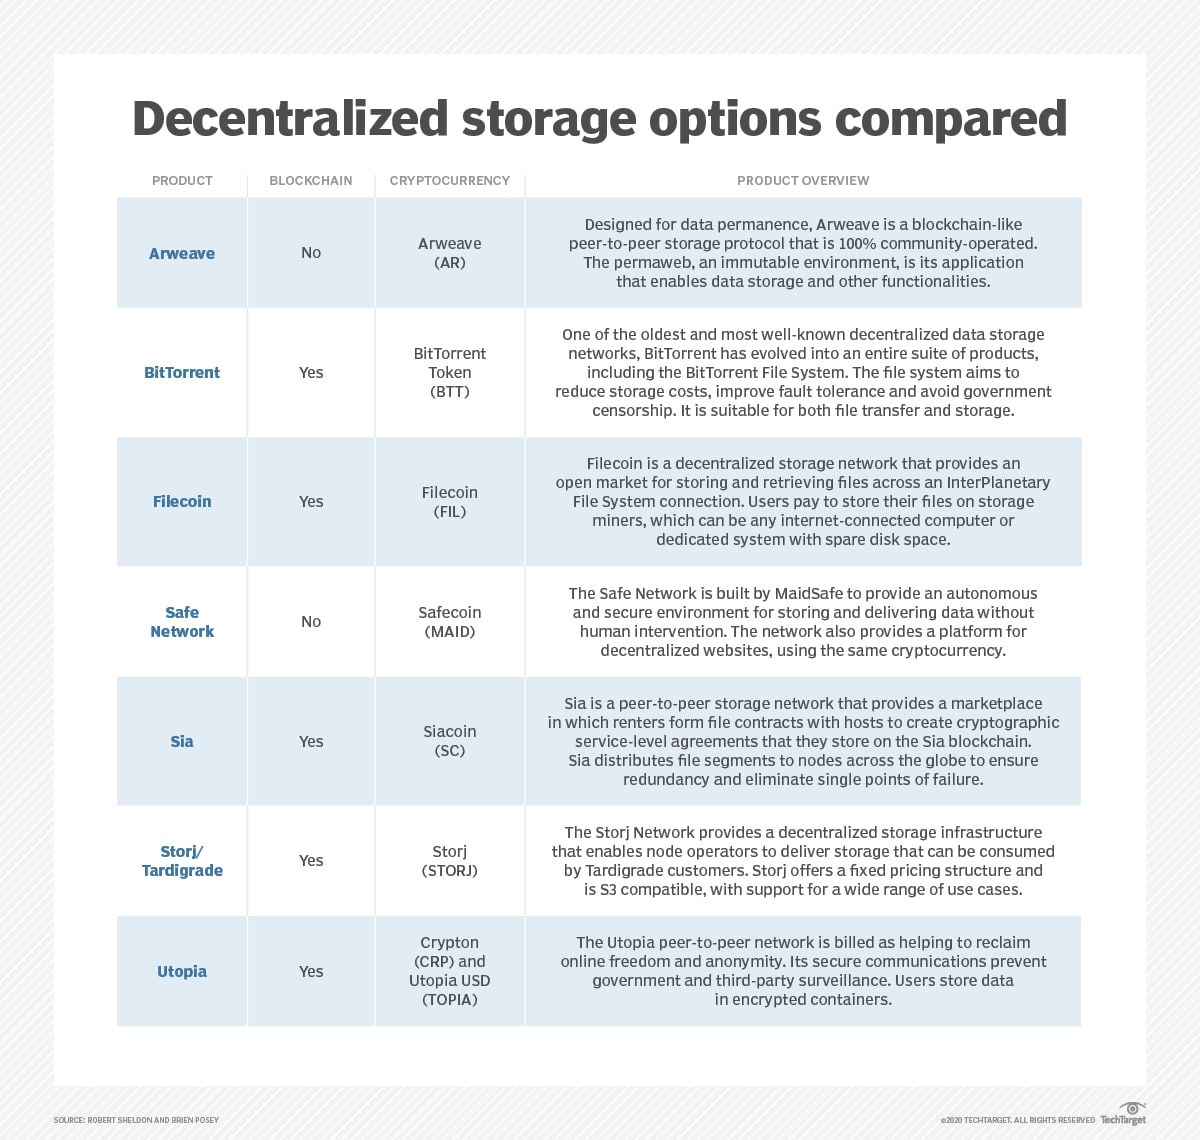
\includegraphics[width=\linewidth]{files}
  \caption{Comparison of distributed file stores}
  \label{fig:Files}
\end{figure}. 
\section{Are DAOs useful for us?}
A distributed autonomous organisation, or DAO is a governance structure which is built in distributed code on a blockchain smart contract system. Token holders have voting rights proportional to their holding. The first decentalised autonomous organisation was simply called ``The DAO'' and was launched on the Ethereum network in 2016 after raising around \$100M. \href{https://www.gemini.com/cryptopedia/the-dao-hack-makerdao#section-what-is-a-dao}{It quickly succumbed to a hack and the money was drained}. This event was an important moment in the development of Ethereum and resulted in a code fork which preserves two separate versions of the network to this day, though one is falling into obsolescence. Again, this is covered in Shin's book on the period in extreme detail, but it seems this stuff is falling into dusty history now, leaving only a somewhat tarnished and technically shaky legacy \cite{cryptopians}. \\
In practice DAOs have very few committed `stakeholders' and the same names seem to crop up across multiple projects. Some crucial community decisions within large projects only poll a couple of dozen eligible participants. Its might be that the experiment of distributed governance is failing at this stage. \par
Perhaps more interesting is the use of the DAO concept to crowd fund global projects, currently especially for the acquisition of important art or cultural items. DAOs are also emerging as a way to fund promising technology projects, though this is reminiscent of the 2017 ICO craze which ended badly and is likely to \href{https://www.cftc.gov/PressRoom/PressReleases/8590-22}{fall foul of regulations}.\par
Within the NFT and digital art space  PleaserDAO has quickly established a strong following.
``PleasrDAO is a collective of DeFi leaders, early NFT collectors and digital artists who have built a formidable yet benevolent reputation for acquiring culturally significant pieces with a charitable twist.\par
Opensea wrangle between IPO and governance token.\par
ConstitutionDAO, Once upon a time in Shaolin etc 
%https://harpers.org/archive/2015/01/come-with-us-if-you-want-to-live/

\subsection{Bisq DAO}
One of the better designed DAOs is \href{https://bisq.network/dao/}{Bisq DAO}. It's slightly different design trys to address the issue of overly rigid software intersecting with more intangible and fluid human governance needs. From their website:\par
\textit{``Revenue distribution and decision-making cannot be decentralized with traditional organization structures—they require legal entities, jurisdictions, bank accounts, and more—all of which are central points of failure.
The Bisq DAO replaces such legacy infrastructure with cryptographic infrastructure to handle project decision-making and revenue distribution without such central points of failure.''}

\subsection{Risks}

The most interesting thing about DAOs is that they belong more in this money chapter than they do in blockchain. As we have seen they're finding most success as loosely regulated crowd funding platforms. If a small company did find itself wishing to explore this fringe mechanism for raising capital, then we would certainly recommend keeping a global eye on evolving regulation and the onward legal exposure of the company. 
\section{Risks \& Challenges?}
Classic DID/SSI risks fragmentations. 
In all DID applications, scaling to a world where the user is managing potentially thousands of these critical cryptographic data files is daunting.
Abstracting the guts of this away to make the use simple, and only mindful of thet right level of information, turns out to be huge problem that nobody has solved
It's not clear that users want this. 
In the case of web of trust like Slashtags it's a big piece of work for the users to rate all of their digital interactions with a trust metric.




\chapter{Non Fungible Tokens}
Nonfungible tokens are a whole `class' of digital token, separate and distinct from everything discussed to this point. They are generally \href{https://www.signaturelitigation.com/nfts-recognised-as-property-lavinia-deborah-osbourne-v-1-persons-unknown-2-ozone-networks-inc-trading-as-opensea/}{recognised in law} as property in their own right \cite{moringiello2021property, fairfield2021tokenized}. In the Initial Coin Offering (ICO) and project tokens detailed earlier, and limiting this description to the Ethereum network for now, a project launching an ERC-20 token commits contract code to the blockchain, and this contract then mediates the issuance and management of millions or billions of tokens associated with that project, and it's use case. \href{https://ethereum.org/en/developers/docs/standards/tokens/erc-20/}{ERC-20} is a \href{https://en.wikipedia.org/wiki/Fungibility}{fungible} token issuance. Each of the projects' tokens is interchangeable with any other token. They're all the same from the point of view of the user.\par
Rather than the ERC-20 contract type used for fungible token issuance NTFs predominantly use ERC-721 protocol on Ethereum (just different instructions). It's the case that most NFTs in the 2021/2 hype bubble are algorithmically generated sets of themed art (so called PFP-NFT). Tens of thousands of distinct tokens are `minted', each one being a complex transaction commitment to the Ethereum blockchain, along with it's associated gas fee. These minting events were much hyped social occasions (before the \href{https://www.theguardian.com/technology/2022/jul/02/nft-sales-hit-12-month-low-after-cryptocurrency-crash?}{2022 market crash}), and happened very quickly, with users clamouring to create art with randomly allocated features from the art schema associated with the project. Lucky winners could find themselves with an NFT art piece with more than an average number of `rare' features. If the overall mint becomes more popular, then the secondary market for all of those mints goes up, and because of the liquidity premium they can go up a lot. The perceived rarer mints go up a lot more. This whole process is \href{https://memoakten.medium.com/the-unreasonable-ecological-cost-of-cryptoart-2221d3eb2053}{very energy intensive} on the chain, and the vast majority of these project simply \href{https://www.turing.ac.uk/blog/non-fungible-tokens-can-we-predict-price-theyll-sell}{trend to zero value}. In response to this appalling cost benefit analysis the Ethereum foundation have proposed \href{https://eips.ethereum.org/EIPS/eip-2309}{EIP-2309} to make minting NFTs more efficient. They say ``This standard lets you mint as many as you like in one transaction!''\par
The Ethereum foundation give their somewhat constrained view of \href{https://ethereum.org/en/nft/}{NFTs on their website} and it's a useful primer. On that page they detail some of the use cases, as listed below, with a critique added:
\begin{itemize}
\item Digital content; this is the dominant use case right now. Much more on this later.
\item Gaming items; again more on this later, it's an obvious enough use case but \href{https://climatereplay.org/nfts/nft-digital-ownership-pledge/}{complex politics} in the intersection of games and crypto have stalled the adoption curve.
\item Domain names; this is just starting to reach for applications now, why not a database with the ISP/host?
\item Physical items; seemed like a clear over-reach as transfer of the NFT does not imply transfer of the object, but this is emerging as the growth use case.
\item Investments and collateral; while this was an emergent option in the space, it's likely been a bubble, as owners of the tokens cast around for additional liquidity, and loan businesses chased yield with higher risk. The \href{https://newsletter.banklesshq.com/p/three-arrows-capital-grayscale-maker-lido}{recent implosion} of lenders and funds in the crypto space was partly a function of supposedly world class risk managers accepting jpegs as collateral.
\end{itemize}
Moving away from Ethereum, NFTs can be minted on most of the other level one chains. Solana is a great newcomer example. Sol is a terrible chain with regards to decentralisation, but thanks to that it's far cheaper and faster to mint NFTs on it, and it was becoming a \href{https://markets.businessinsider.com/news/currencies/ethereum-eth-killers-nfts-defi-solana-cardano-wax-crypto-investing-2022-1}{troubling competitor} for Eth before the FTX ponzi scheme collapse destroyed it's market value (Figure \ref{fig:solnfts}).\par 
\begin{figure*}[ht]\centering % Using \begin{figure*} makes the figure take up the entire width of the page
	\includegraphics[width=0.7\linewidth]{solnfts}
	\caption{Solana NFT markets are enjoying growth compared to Opensea on Ethereum, even in the downturn.}
	\label{fig:solnfts}
\end{figure*}
The same might be true for Cardano's ADA, though ADA is struggling to hold onto it's market position despite some technical advances. It's worth reiterating here that the nature of these digital tools likely makes for a `winner take all' market dynamic over time. With fees being central to this generative NFT use case it's possible to see that highly centralised, fast, and cheap chains will capture and eventually dominate the space. Remember that this likely (game theoretic) outcome might as well be a database running without the stark inefficiencies of blockchain. The whole NFT space is a gamble on consumer enthusiasm for spending money continuing to outpace logic.\par 
Astonishingly, according to a JPMorgan insider market report (\href{https://www.coindesk.com/podcasts/the-breakdown-with-nlw/jpmorgan-bitcoin-shows-some-merit-as-a-store-of-value/}{reported on in a podcast}), only around 2 million people have ever actually interacted with NFTs. One analysis suggests that a single entity accounts for 3 of the top 4 holders, having made 32,000 ETH from the NFT boom. This suggests heavy market manipulation and is far from the egalitarian landscape claimed in the hype. Tellingly it's thought around \href{https://uk.finance.yahoo.com/news/three-arrows-wanted-100m-nft-161811450.html}{10\% of the trading volume} on market leading platform `Super Rare' was by the now bankrupt venture capital firm `Three Arrows'. \par
With that said NFTs have clearly allowed \href{https://en.wikipedia.org/wiki/List_of_most_expensive_non-fungible_tokens}{digital and new media artists} to connect with audiences without gatekeepers. Established mediators and curators of art have been caught totally wrongfooted, and NFTs seem to give a way for them to be cut out completely. There are suggestions of applications beyond this initial digital art scope. This is a compounding, and disrupting paradigm change.\par
%Users of NFT markets have \href{https://blog.chainalysis.com/reports/nft-market-report-preview-2021/}{injected around \$30 billion into the tokens during 2021}. 
\section{Key use cases}

\subsection{Art}
The recent surge of interest in NFT's during early 2021 has largely been
driven by digital art NFT's, despite the origins of digital art NFT's
started much earlier in 2014. New York artist \href{https://www.mccoyspace.com/project/125/}{Kevin McCoy's
\emph{Quantum}} is widely recognised as the first piece of art created
as an NFT. However it was during early 2021 that art NFT's started to
gain significant attention; by the end of 2021, nearly \href{https://www.paymentscardsandmobile.com/state-of-the-blockchain-nfts-explode-onto-scene-in-2021/}{£31b
had been spent} on NFT purchases, a considerable and exponential growth
given \href{https://raritysniper.com/news/nfts-exploded-in-2021-with-25-billion-in-sales/}{2020
sales of \textasciitilde£71m}
High profile digital artists such as \emph{Beeple} whose
\href{https://www.forbes.com/sites/abrambrown/2021/03/11/beeple-art-sells-for-693-million-becoming-most-expensive-nft-ever/?sh=3f237d1c2448}{recent
recording break sale} of his NFT \emph{``The first 5000 days''} (Figure \ref{fig:first5000days}) at Christies (a long established British auction house,
specialising in high profile precious work of art) for £52.9m helped
bring NFT's into the public spotlight and wider give them global
attention.

\begin{figure*}[ht]\centering % Using \begin{figure*} makes the figure take up the entire width of the page
	\includegraphics[width=\linewidth]{first5000days}
	\caption{Beeple: First 5000 days, \href{https://onlineonly.christies.com/s/beeple-first-5000-days/lots/2020}{taken from the Christies website, assumed fair use}.}
	\label{fig:first5000days}
\end{figure*}

Art as NFT's offer the following advantages:

\subsubsection{Immutable Nominal Authenticity} 
Art fraud such as false
  representation, forgeries, plagiarism have been a reoccurring blight
  since art has existed; artists and works of art have been open to
  abuse by forgers, black market profiteers and even fellow artists
  laying claim to works of art of others. Unless a work of art is sold,
  exhibited or listed, documenting when and who created it, the
  \emph{nominal authenticity,} which Dutton states as the
  \emph{``correct identification of the origins, authorship, or
  provenance of an object''} \cite{dutton2003authenticity} can be increasingly mutable over a period
  of time, dependent on a multitude of factors, including; the artists
  existing profile, how widely and where the work of art is exhibited,
  if the work of art is commissioned by a patron, if it's sold, and
  profile of the buyer/collector. At its most basic level, once a work
  of art is `minted' as an NFT (publishing the art work as a unique
  token on the blockchain) this functions as an immutable publicly
  accessible proof of ownership and by extension proof of creation. The
  act of minting is not purely limited to digital art; all an artist
  requires is a digital representation of any physical art (sculpture,
  physical painting, installation etc..) which can be used as a proxy
  allowing artists to record the date of creation/origin of a physical
  piece of art on the blockchain, a buyer purchasing the NFT can be
  provided the actual physical artwork as part of the NFT. Nominal
  authenticity becomes secure and immutable for the lifetime of the blockchain (by no means assured).

\subsubsection{Secure Digital Provenance}
\href{https://en.wikipedia.org/wiki/Provenance}{Provenance} (or the chain of custody) is an important aspect in works of art, antiques and antiquities. Provenance not only helps assign work to an artist but also documents ownership history. Digital provenance, an inherent feature of NFT's means provenance now no longer becomes what has historically sometime been a contentious detective's game at the best of times; one that is open to fraud, misinterpretation and entirely reliant on good record keeping.\par
Since provenance can contribute to the value of a piece of art (benefiting both the creator and collector) the use of the blockchain as an open, secure ledger is a far more trustworthy system than traditional methods of artistic provenance that were cobbled together; often
consisting of a mix of physical and digital documents spanning private
\& public sale receipts, art/museum gallery exhibitions and private
record keeping). Digital provenance provided when an artist `mints' a
piece of art into an NFT allows artists and collectors to record a
secure, permanent unalterable history of transactions for a specific
piece of art, providing future collector complete trust in the origin
and custody of a piece of art.
\subsubsection{Decentralised automated royalty payments} 
Traditionally if a  piece of art is sold, the first sale may (but not always) benefit the
  artist financially, however secondary and any subsequent sales would
  only ever financially benefit the buyer/collector; the original artist
  would rarely benefit. However If a work of art is minted into an NFT,
  royalty payments can be predetermined and automated in perpetuity
  directly by the use of a `smart contract'. Smart contracts are small,
  automated scripts/programs that run automatically and independently of
  a buyer/seller; pre-determined conditions are set by the buyer; these
  trigger when certain conditions are met i.e. These cannot yet be enforced ``on chain'' and the NFT auction houses online have engaged in a race to the bottom and stopped enforcing royalty payments through their systems. This element might not even be possible, though there is some hope that we could enable this in the complex logic offered by the RGB protocol.
\subsubsection{On sale transfer}
20\% of total sale amount into digital wallet of the creator.
80\% of total sale amount into digital wallet of the seller.

Once the royalty payment rate is set by the artist/creator, future
royalties of all sales can be paid directly to the artist/creator
account (via a digital wallet) without the need of a third party
(traditionally a gallery/agent etc..).

Smart contract driven NFT's means that even if piece of art is resold 5,
10 or even a 100,000 times moving through 5, 10 or even a 100,000
different collectors; a pre-determined royalty payment rate set by the
creator would still guarantee the artist/creator is paid directly from
each and every future sale.

Historically provenance for works of art may span across generations,
for instance Gabriël Metsu's oil on canvas painting \emph{The Lace
Maker's} provenance, first recorded in 1722, now spans 300 years of
ownership, including from a British Baron in the 19\textsuperscript{th}
century to an American philanthropist in the 20\textsuperscript{th}
century.) Metsu died young at the age of 38, leaving a widow; neither
his/her relatives/descendants benefit from his original work, 300 years
later this would be near impossible to facilitate with traditional
systems, as even legal contracts are open and prone to the ravages of
time.

NFT smart contracts hold an incredibly potential; an artists descendants
financially benefiting directly from the resale of a piece of work long
after the artist/museum's/gallery or even state have turned to dust as
long as the original creator's digital wallet is accessible, \emph{the
blockhain becomes an everlasting digital patron} ensuring


NFT art currently suffers from the same failure of decentralisation already discussed in the Ethererum technology stack, but this is compounded by the normalisation of intermediate art brokers \href{https://moxie.org/2022/01/07/web3-first-impressions.html}{continuing to custody} the NFTs even after sale. They are usually selling a pointer to their own servers. The market is nascent and evolving, but it's currently not delivering on it's core promise.\par
Proof of ownership is intuitively a pretty obvious application for the technology, but again it's hard to justify the expense when the benefits are so slim. \href{https://www.bullishlybred.com/}{Bulldogs on the blockchain} is a clear gimmick, and might even incentivise poor behaviours as there are two products here which are not necessarily aligned. Much has been written over the years about \href{https://propy.com/browse/propy-nft/}{deeds to property} being passed through blockchains, cutting out the middle man, but in the event that a house deed NFT was hacked and stolen it's obviously not the case that the property would then pass to the hacker.\par 
One of the most interesting companies is Yuga Labs, who launched the incredibly popular Bored Ape Yacht club set of 10,000 algorithmically generated NFTs. These Ethereum based NFTs were based loosely on the `Crypto Punks' model of PFP-NFT (variously profile picture project, picture for proof, and picture for profile - no definition remains uncontested for long). Yuga launched with a better commercialisation model for the holders, and a strong marketing drive into celebrity circles. They now regularly change hands for hundreds of thousands of pounds. Even this `blue chip' NFT is not without \href{https://twitter.com/coryklippsten/status/1538909505236283392}{serious criticism}: \textit{``I'd put it at 99.99\% the project is in fact a deliberate troll, intentionally replete with Nazi symbols and esoteric racist dog whistles''}\par
Yuga recently bought the artistic rights to the commercial reuse of similarly popular (and preceding) Punks set. This is interesting because they have again handed the commercial re-use rights to the owners of the individual NFTs. This raises the same \href{https://www.bloomberg.com/news/articles/2022-03-21/bored-ape-nft-spinoff-venture-gone-sour-sparks-legal-fight}{confusing problem} with attaching commercial rights to an easily stolen token as NFTs for real estate does. This has been demonstrated recently when Seth Green had a Bored Ape stolen after \href{https://www.buzzfeednews.com/article/sarahemerson/seth-green-bored-ape-stolen-tv-show}{creating an animated show around it's IP}. Many more contradictions and ambiguities in NFT licenses are emerging. Galaxy Digital have \href{https://www.galaxy.com/research/insights/a-survey-of-nft-licenses-facts-and-fictions/}{surveyed the landscape}:
\textit{``Contrary to the ethos of Web3, NFTs today convey exactly zero ownership rights for the underlying artwork to their token holders. Instead, the arrangements between NFT issuers and token holders resemble a distinctly Web2 maze of opaque, misleading, complex, and restrictive licensing agreements, and popular secondary markets like OpenSea provide no material disclosures regarding these arrangements to purchasers. Something more is required, and that `something' is a legal agreement between the owner of the image—known as the `copyright holder' and the NFT holder specifying what rights the NFT holder has with respect to the image. To the extent an NFT purchaser has any rights to the image associated with his or her NFT at all, those rights flow not from his or her ownership of the token, but from the terms and conditions contained in the license issued by the NFT Project governing the NFT holder’s purchase and use of the image. Accordingly, for the vast majority of NFT projects, owning the NFT does not mean you own the corresponding digital content that is displayed when you sync your wallet to OpenSea. That content, as it turns out, is owned and retained by the owner of the copyright associated with that digital content, typically the NFT project.
After reviewing the most used license agreements for NFT projects, it becomes apparent that NFT standards and smart contracts do not recognize off-chain law.''} There may already be a response from the industry to this in the shape of \href{https://a16zcrypto.com/introducing-nft-licenses/}{a16z's ``can't be evil'' license proposal}.\par
Even so, the community around these collections is incredibly strong, mixing developers, artists, the rich and famous, and the fortunate and early, into a cohesive community who communicate online. The developer `good will' is enormous, and it seems possible that this will lead to faster and broader innovation around the collections, and out into \href{https://twitter.com/yugalabs/status/1505014986556551172?}{metaverse applications}. The brand is strong, and the individual NFT items both benefit from, and reinforce that brand, while adding personal narratives and human interest.\par 
As a gauge of how frothy this market still is it's interesting to look at the APE token which Yuga just launched. They airdropped 10,000 of the tokens free to each of the 10,000 NFT holders. This instantly created a multi-billion dollar market cap, and a top 50 `crypto' out of thin air, based purely on their brand. It's clear that there is both brand, and a market here.\par
A recent report from "Base Layer" tries to capture the community `feature' of big brand NFTs. \href{https://baselayer.so/crypto-culture-decoded}{``Crypto culture decoded''} explains that is is these online communities which are the attraction not necessarily the art. This is a powerful `in group' argument, though speculation remains the most likely underpinning.\par

%\href{https://amycastor.com/2021/03/14/metakovan-the-mystery-beeple-art-buyer-and-his-nft-defi-scheme/}{Beeple scam}

While it is likely that this is currently a speculative bubble, that is \href{https://www.bbc.co.uk/news/business-61102759}{waning already} (Figure \ref{fig:monkey}), it seems certain that the technology is here to stay in some form.\par

\begin{figure*}[ht]\centering % Using \begin{figure*} makes the figure take up the entire width of the page
	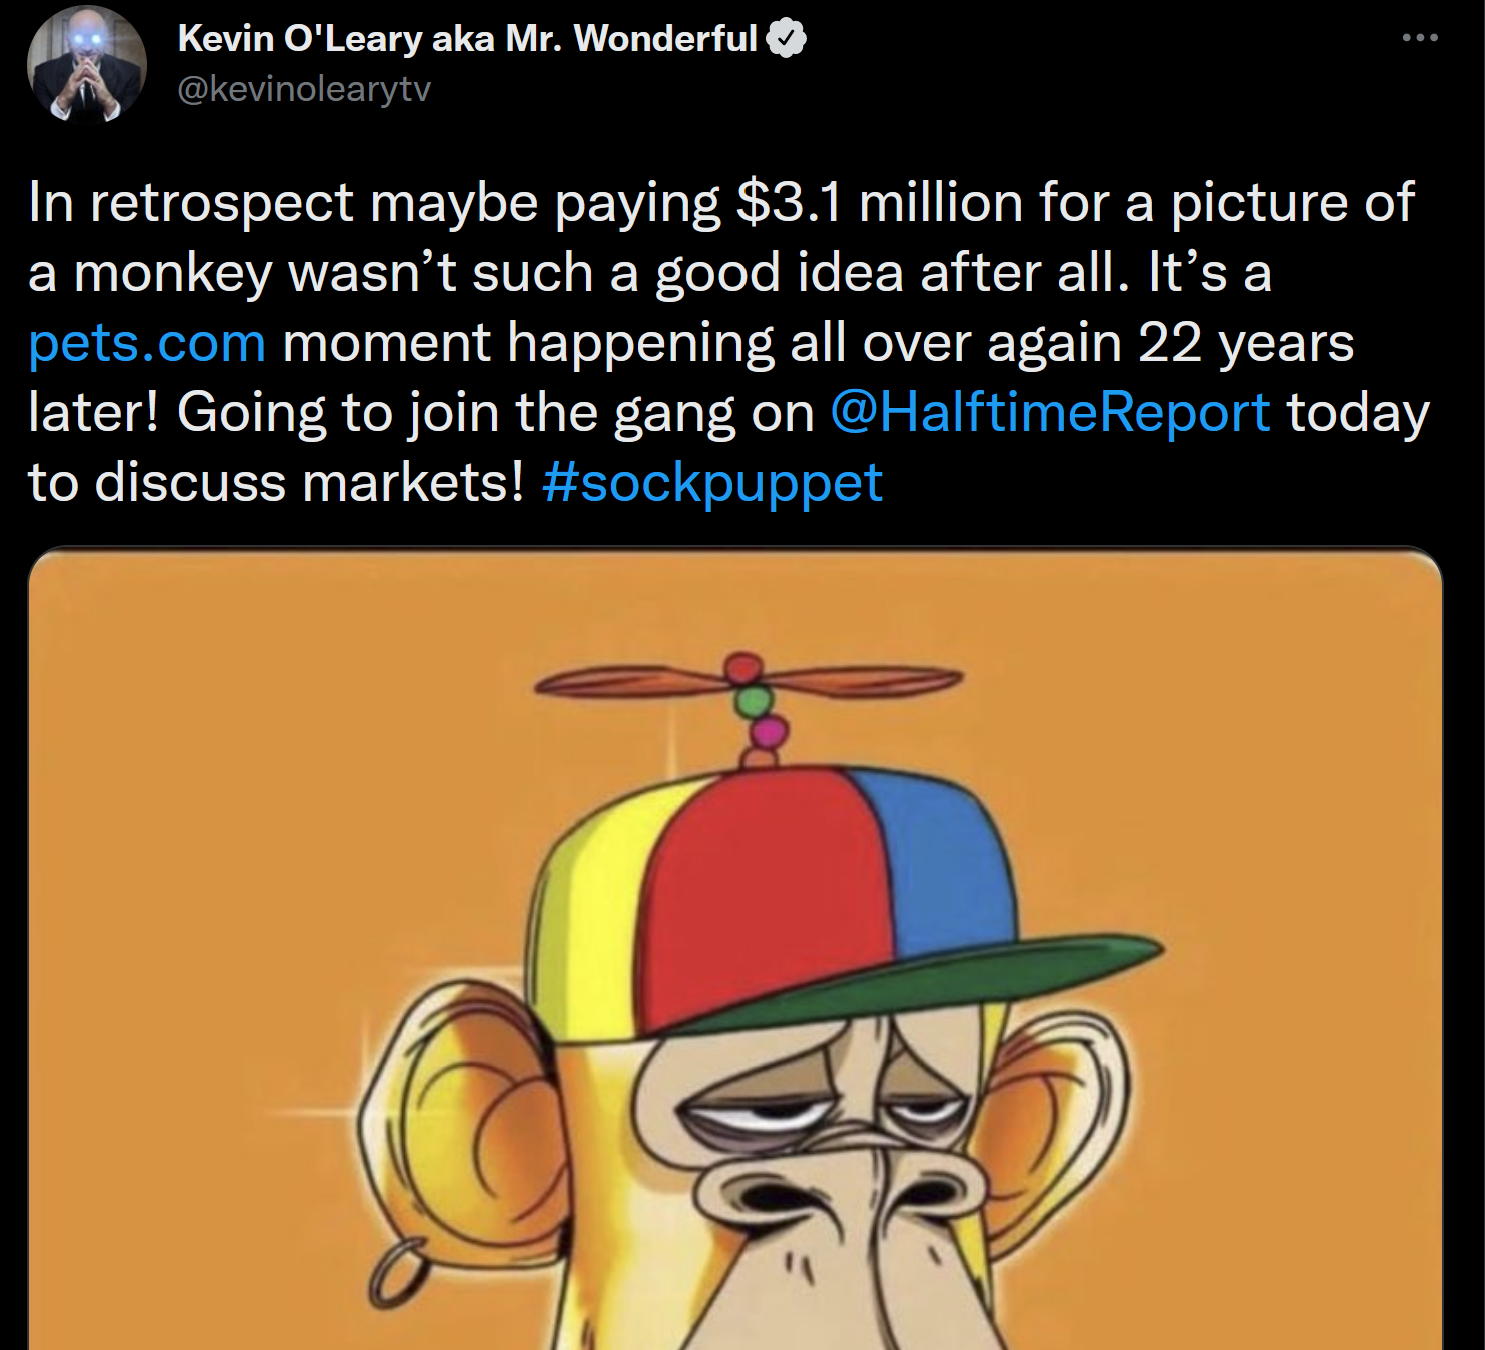
\includegraphics[width=\linewidth]{monkey}
	\caption{The \href{https://www.coingecko.com/en/nft/bored-ape-yacht-club}{bubble bursts} on Yuga Bored Apes for now.}
	\label{fig:monkey}
\end{figure*}


\subsection{Computer \& Video Games}
Computer \& Video games are a huge global business, exponential global
growth over the last 30 years has seen this grow to a point where it has
eclipsed both the
\href{https://www.businessinsider.com/video-game-industry-revenues-exceed-sports-and-film-combined-idc-2020-12?r=US\&IR=T}{global
movie and North American sports industries} combined.

A global industry with revenues over £120b,
\href{https://www.wepc.com/news/video-game-statistics/}{with
\textasciitilde half the people on the planet} playing some form of
games in 2021.

As the games industry has evolved and matured over the last 40 years,
secondary markets have emerged, most notably the `second hand' games
resale market. The rise of `retro' gaming, has demonstrated the second
hand market is a lucrative one for private resellers, an unopened copy
of Super Mario Bros for the Nintendo Entertainment System
\href{https://www.nytimes.com/2021/08/06/business/super-mario-bros-sale-record.html}{recently
selling for £1.5M} to the extent the market has seen
\href{https://www.businessinsider.com/retro-gaming-market-being-overtaken-by-speculators-2021-9?r=US\&IR=T}{speculators
looking to cash in} on the huge global interest in retro/second hand
games.\par
Despite publishers and developers increasingly moving to non-physical
digital only' games, the demand for used games remains incredibly high.\par
Whilst some retailers have adapted their business models to include reselling of retro/second hand games, the vast majority of publisher/developers/retailers aren't able to directly benefit from the
emerging retro/second hand games market. The potential of \emph{video
games as NFT's} presents a huge opportunity for publishers, developers
and players alike, offering the following advantages:
\subsubsection{Royalty Sales on Pre-owned Games} ; A predetermined proportion
  of any resale of a used game can automated in perpetuity via smart
  contracts; once these are set by the publisher, future royalties of
  all sales can be paid directly to the publishers/developers wallets (a
  digital account) without the need of a third party (traditionally a
  retail entity). Traditionally only the initial first sale of a game
  would financially benefit the publisher/developer/retailer, secondary
  and subsequent sales would only ever financially benefit the
  purchaser, with many developers/publishers arguing this is hurting the
  wider industry through the loss of significant income generated by the
  secondary and subsequent sales, sometimes over the course of decades.
  However the use of NFT's smart contracts means that if a game is
  sold/resold through 10,000 collectors; a pre-determined royalty
  payment rate set by the publisher would still guarantee the publisher
  (and or developer/retailer) takes a proportion of any future sales.
\subsubsection{Monetisation of User Generated Content:} Games as a NFT's
  offer ability to monetise UGC: User generated content. Video games such as
\href{https://www.businessofapps.com/data/pokemon-go-statistics/}{Nintendo's
\emph{Pokemon Go}} \emph{(166 million players)},
\href{https://techacake.com/destiny-2-player-count/\#:~:text=The\%20total\%20player\%20base\%20of,to\%20be\%2038\%20million\%20players.\&text=According\%20to\%20the\%20source\%2C\%20the,in\%20terms\%20of\%20player\%20population.}{Bungie's
\emph{Destiny 2}} \emph{(38 million players)} or
\href{https://fictionhorizon.com/how-many-people-play-genshin-impact/\#:~:text=Genshin\%20Impact\%20had\%20approximately\%209,million\%20users\%20in\%20June\%202021.}{miHoYo's
Genshin Impact} (\emph{9 million players} ) all have large, established
and significant player bases. What is noteworthy, the games are designed
to encourage players may spend hundreds, or in some cases thousands of
hours on one game alone; according to
\href{https://destinytracker.com/destiny/leaderboards/all/minutesplayedtotal?grouped=true\&page=1}{Destinytracker.com},
the top players have amassed total play times over 20,000 hours, close
to 1,000 days or \textasciitilde{} 3 years, which is incredible feat
given Destiny 2 only launched 5 years ago in 2017.\par
Destiny/Pokemon Go and Genshin Impact revolve around a central key game
mechanic; players investing significant amounts of time collecting in
game digital assets; characters/weapons/items, often classed as `rare'
or `exotic' or `5 Star'. These collectibles usually found by a
combination of the accrual of in-game time, completing quests,
purchasing additional in-game items/boosters, and luck (`RNG'). Players
are often encouraged to share their collections of rare
characters/weapons/ objects through in-game achievements, triumphs,
scores acting as a mark of distinction/status symbol.\par
Traditionally there has been nothing that went beyond sharing the
\emph{digital badge} (i.e triumph/achievement/accomplishment) on a on
social media/gamer's platform profile. However NFT's offer the ideal
system for developers/publishers and even players to monetise user
generated/customised data (such as a players unique save game data), simultaneously allowing:
a) creation of an additional monetised ecosystem to meet player demands
i.e. some players who are willing to monetise and `sell' their invested
time in a particular product/service to other players with little time
but willing to pay other players for `grinding' (progressing laborious
in game tasks) and a more advanced in-game progression point.
The potential to provide publishers/developers with an additional
long-term income stream, providing a better ROI on computer \& video
game development, which in many instances can cost hundreds of millions
in development costs spanning 5/10 years, is undeniable.
\subsubsection{Play to earn revenue models}
This is morally dicey at this time and early startups like \href{https://www.bloomberg.com/news/features/2022-06-10/axie-infinity-axs-crypto-game-promised-nft-riches-gave-ruin}{Axie Infinity are in serious trouble}. A (long) \href{https://www.youtube.com/watch?v=YQ_xWvX1n9g}{video by Dan Olsen} highlights the structural problems with both play to earn and NFTs. On chain analysis suggested that 40\% of accounts in 200 current Web3 games \href{https://gallery.usejigger.com/}{are bots}. 
\subsubsection{Monetizing In game collectibles}
customisable in game assets (vanity
  items such as cosmetic character skins/clothing or collectible items
  that offer player advantages(new weapons/vehicles/mods etc,..)



Traditional gamers have pushed back on the seemingly useful idea of integrating NTFs with traditional games. This may be in part because Ethereum mining has kept graphics card prices high for a decade.

\href{https://www.prnewswire.com/news-releases/hbar-foundation-and-ubisoft-partner-to-support-growth-of-gaming-on-hedera-network-301474971.html}{HBAR partnerships}\par
\href{https://finance.yahoo.com/news/epic-games-vp-people-have-lost-interest-in-the-metaverse-200725562.html}{Critique from Marc Petit of Epic and Unreal}.\par
The \href{https://twitter.com/justinkan/status/1491270239967154178}{following text} is from Justin Kan, co-founder of twitch: \textit{``NFTs are a better business model for games. Many gamers seem to be raging hard against game studios selling NFTs. But NFTs are also better for players. Here’s why I think blockchain games will be the predominant business model in gaming in ten years. NFTs are a better business model for funding games . Example: recently I invested in a new web3 game SynCityHQ. They are building a mafia metaverse and raised \$3M in their initial NFT drop.\\ NFTs give studios access to a new capital market for raising capital from the crowd.NFTs can be a better ongoing model for games. Web3 games will open economies, and by building the games on open and programmable assets (tokens + NFTs) they will create far more economic value than they could from any one game. Imagine Fortnite, but other developers can build experiences on top of the V-Bucks and skins. Epic would get a royalty every time any transaction happens. As big as Fortnite is today, Open Fortnite could be much bigger, because it will be a true platform. NFTs are better for gamers Allowing gamers to have ownership of the assets they buy and earn in game allows them to participate in the potential growth of a game. It lets gamers preserve some economic value when they switch to playing something new. But what about the criticisms of NFTs?\\
Here are my thoughts on the common FUDs: "It’s just a money grab on the part of the studios!"\\
Game studios already switched over to the model of selling in-game items, cosmetics, etc to players long ago. But currently the digital stuff players are buying isn’t re-sellable. NFT ownership is strictly better for players. "The games aren’t real games." This reminds me of the criticism of free-to-play in 2008, when the games were Mafia Wars / FarmVille. We haven’t had time for great developers to create incredible experiences yet. Everyone investing in games knows there are great teams building. "Game NFTs aren’t really decentralized because they rely on models / assets inside centralized game clients."
Crypto is as much a movement as it is a technology. Putting items on a blockchain is what gives people trust that they have participatory ownership...which make people willing to buy in to the game. These assets are “backed” by blockchain.
The fact that these item collections are NFTs will make other people willing to build on top of them. "NFTs are bad for the environment." Solana and L2s solve this. NFT games are better for players and for game developers. Like the free-to-play revolution changed gaming, so will blockchain. The games of the future will be fully robust, with open and programmable economies.}''
\section{Broader and metaverse uses}
So far according to a16z NFTs break down into:
\begin{itemize}
\item Profile pictures: These were discussed at the start of the chapter and have felt ubiquitous on Twitter over the last couple of years. The major projects will likely hold value, but the hype cycle will likely lead to all profile NFTs going in and out of fashion. There's potentially a fresh wave of this same kind of low key identity hype possible in the metaverse, and indeed the two plausible both intersect and converge.
\item Art and Music: Art has also been discussed above. Peter Thiel, the billionaire venture capitalist who founded PayPal has invested in expanded NTF use cases. The first is `Royal' which is experimentally \href{https://royal.io/}{selling limited NFT tokens} which contractually entitle the holder to a portion of music artist royalties. Spotify are experimenting with music NFTs (and of course in the metaverse). This is an early adopter area, and again likely converges with our planned uses cases as more complex tooling appears. For instance Tim Exile of \href{https://endlesss.fm/}{Endless.fm} talks about digital assets extending to the building blocks of co-created music, and wished to build a music creator economy which distributes value to creators at the instant of the final value transaction with the consumer.
\item Gaming: As discussed there's pushback from the gaming community, but huge investment from the likes of Lego, Blizzard, Epic, Ubisoft etc.
\item Gig tickets: Not only the straightforward use of \href{https://news.yahoo.com/psg-sells-us-220-000-030927515.html}{transferable tickets for events} as NFTs on a blockchain (which is impossible due to the cost right now) but also onward monetisation of ticket stubs as memorabilia. The NBA is \href{https://deadspin.com/investing-in-nft-ticket-stubs-is-likely-one-of-the-nba-1848991991}{already looking at this}.\\
\textit{``The team sells the ticket for face value many many years ago, but when that stub is being sold now for much more many times over, the team gets none of that money,'' York explained. ``But with an NFT stub that changes. Let’s say a new rookie enters the NBA next season and he turns out to be the next LeBron James. That ticket stub from his first game, as an NFT, the team can put a commission on it — 20 percent or however much, the NBA decides that. In 10 years when it’s worth a lot of money, I or whoever owns that NFT, can sell it for say \$100,000. The NBA can still collect 20 percent of that sale, because it’s all on a smart contract.''}\par
It seems so obvious that this will extend to the virtual events space in the metaverse.
\item Utility: These are broadly `membership' style tokens, and this seems like a sensible fit. Peter Thiel (again) for instance launches a \href{https://www.ztonft.com/}{political funding NFT} from Blake Masters to support his senate ambitions. To be clear, Thiel is a fundamentalist libertarian, and at the very least \href{https://gizmodo.com/peter-thiel-bitcoin-talk-miami-2022-1848764790}{highly eccentric}. This is not necessarily a positive for the technology.
\item Virtual worlds are a huge application for NFTs, and this seems like it would be a natural fit for out metaverse application. In reality the \$2B of sold so far is mostly `allocations' in nascent ecosystems, being sold as highly speculative assets, without even a metaverse to use. The majority of that amount is the hyped `Otherland' plots sold under the Bored Apes brand.
\item ``Full stack'' luxury brands. \href{https://medium.com/@nic__carter/redeem-and-retain-nfts-are-the-future-of-luxury-goods-760f00dbce23}{Nic Carter describes} a mating of physical and virtual luxury goods. His is a useful article on the future direction, and he has also \href{https://medium.com/@nic__carter/why-nfts-are-hard-to-explain-48f0ab0a35bf}{provided a primer on NFTs}. There are many such examples already, such as \href{https://nft.tiffany.com/faq/}{Tiffanys `NFTiff' - cryptopunks} collaboration which will automatically generate royalties for Tiffanys and parent company Louis Vitton in perpetuity. Such products prove provenance, create new aftermarket opportunities, and unlock metaverse applications.
\end{itemize}
It is completely reasonable to assert that these use cases could be accomplished without the use of NFT technology, and is part of the hype bubble.\par
Twitter user Cantino.Eth offers an exhaustive roundup of what they think future uses might be. It's a \href{https://twitter.com/chriscantino/status/1542930648750608387}{thread full of industry insider jargon} but it's indicative of a shift in focus from speculation to `building' as the market conditions change. Some of the more interesting (less arcane) use cases identified in the thread are summarised very briefly below, again with comments as to how this might pertain to our metaverse applications.
\begin{itemize}
\item Hobby tokens, demonstrating interest in an activity. This is potentially a metaverse adaptation of badges on a blazer in the real world, and might serve to drive communities in a metaverse. The same is true for activism and political alighnment. It's a great idea and worth developing.
\item Professional Networks and qualification badges, like a LinkedIn qualification panel, but in the metaverse. A cisco NFT in the metaverse for a CCNA qualification makes intuitive sense. 
\item Badges to indicate membership of distributed projects within a metaverse. This allows users to identify avatars with shared goals in the metaverse.
\item Retail incentives, like brand loyalty stamps or rewards for participation in marketing, or early access programmes. This is a true in a metaverse marketplace as it is in a real world coffee shop.
\item Multiplayer communities with incentives to hit collective milestones. ``Collecting as a team sport''. This again seems like a great and intuitive opportunity, but is perhaps less suitable for our more business focussed space.
User content submission and automatic monetisation when reused by brands, bonded to an NFT contract.
\item Customer Cohort NFTs: early adopters of successful brands would be able to prove the provenance of their enthusiasm for a new product, and this might unlock brand loyalty bonuses. It seems this wouldn't be a transferable NFT, and is more like the ``soulbound'' idea advanced by Meta.
\item Education and Customer Support, think an NFT of a great score on reddit community support forums. A trusted community member badge, but visible in the metaverse. This is somewhat like the web of trust model advanced earlier in the book.
\item NFTs as contracts is far more likely in the metaverse than it has proved to be in real life. This is how `digital land' and objects will be transferred anyway, but with the addition of contractual conditionals with external inputs more subtle products may appear.
\end{itemize}
%Samsung for instance have announced that their TVs will support not only \href{https://news.samsung.com/us/samsung-2022-micro-led-neo-qled-lifestyle-tvs-personalization-options-ces-2022/}{display of NFTs} with artist defined settings in the metadata, but also an integrated marketplace for browsing and purchasing.\par

\section{Objects in our metaverse}
There has been a recent shift away from the `toxic' moniker of NFT and toward `Digital objects', and seem to be judged crucial to metaverse applications. The success of avatar `collectibles' markets in the Reddit ecosystem, and Meta (ex Facebook) similarly divesting themselves of the NFT term seem to suggest a pivot point in the industry. Meta are encouraging adoption through zero fee incentives but are likely hanging their monetisation of their whole rebrand on taking a huge cut from NFT content creators on their platform. Crucially for the whole concept of NFTs in crypto it looks like they will custody the digital objects within their databases, and allow them to be both bought and sold through interactions with `normal' Fiat money. This completely breaks the model of what an NFT represents, and may in time dilute the technology to the point of being completely meaningless.\par
We have a path to assets and NFTs within the layer 3 elements of our choice (RGB \& Pear Credits), but they're not yet fit for purpose. There are compromise options already available, as below. 
\subsection{Liquid tokens}
We have seen that Liquid from Blockstream is a comparatively mature and battle tested sidechain framework, based upon Bitcoin. It is possible to issue tokens on Liquid, and these have their own hardware wallet available. This makes the technology a strong contender for our uses.
\subsection{Sovryn and RSK}
It's slightly unclear when RSK will support assets at this level. This needs to be revisited.
%\subsubsection{Optimistic rollups}
%\lipsum[50]
%\subsubsection{Zero Knowledge rollups}
%\lipsum[50]
\subsection{Stacks and STX}
There's another possible option is Stacks, without the network effect of Ethereum, but closer to the other design choices made so far. ``Stacks is an open-source network of decentralized apps and smart contracts built on Bitcoin.''\\ 
This novel approach saw the launch of a layer 1 blockchain token called STX, which is used in a similar way to gas in Ethereum. but claims settlement on the Bitcoin network. This is achieved through a novel bridging approach which they call Proof of Transfer (PoX).\\
Stacks users say this hybrid approach is a pragmatic solution which enables dApps, smart contracts, DeFi, NFTs etc without compromising security. In practice the speculative component of the STX tokens which underpin these operations clouds the issue somewhat. It is a potentially useful middle ground solution with a great deal of developer attention.
\subsection{Ethereum}
While it's been discounted elsewhere it's hard to ignore the network effect of Eth NFTs. If the aspiration is to attract the bulk of the `legacy' creator/consumer markets then it will be necessary to support integration of Metamask into any FOSS stack. This isn't a huge technical challenge, nor is it particularly of interest to our use cases at this stage, but it remains a possibility. The main problems remain the slow speed and high expense of the system.
\subsection{Solana}
Solana is both cheap and fast, because it's very highly centralised. It seems unlikely that it's worth this level of compromise. It has also become embroiled with the fallout from the enormous FTX exchange fraud, threatening the existence of the assets (NFTs) issued and stored upon it.
\subsection{Satoshi Ordinals}
Satoshi ordinals \href{https://github.com/casey/ord}{allow tracking of Sats across transactions}, enabling NFT like assignment tracking. This is a hugely exciting development but extremely early.
\subsection{Peerswap}
It may be possible to use ``Peerswap'' to execute rebalancing and submarine swaps into and out of Liquid assets on the sidechain in a single tx. This is anunder explored area at this time.
\subsection{FROST on Bitcoin}
It \textbf{might} be possible to transfer ownership of a UTXO on the Bitcoin base chain using FROST \cite{komlo2020frost}. In this Schnorr \& Taproot based threshold signature system it's possible to \href{https://btctranscripts.com/sydney-bitcoin-meetup/2022-03-29-socratic-seminar/}{add and remove signatories} and thresholds of signing without touching the UTXO itself. In principle (though not yet in practice) this might allow transfer of UTXO ownership. 
\subsection{Spacechains}
It feels like spacechains are almost ready, so this is worth keeping an eye on. It's the `cleanest' way to issue assets using Bitcoin because there's no additional speculative chain. As briefly explained in the earlier section Bitcoin is destroyed to create a new chain which then inherits the security of Bitcoin through onward mining. This new asset or chain is able to accrue value and trade independently based purely on it's value to the buyer, not as a function of a wider speculative bubble attached to a token with multiple use cases.
\subsection{Pear credit}
The outstanding contender at this stage is Pear Credit from Hypercore. This section needs a full explanation later. For now a \href{https://medium.com/@observer1/tether-announced-the-launch-of-pear-credit-8d4f66ccd97b}{blog post on the subject} will have to do.


\chapter{Metaverses}
\section{Toward an open metaverse}
For our purposes in this book and product design the interface between the previous chapter (NFTs) and this metaverse chapter is crucial. Punk6529 is a pseudonymous twitter account and thought leader in the ``crypto'' space. The text below encapsulates much of the reasoning that led to this book and product exploration, and is paraphrased \href{https://twitter.com/punk6529/status/1536046831045685248}{from this thread} for our purposes.\par
\textit{Bit by bit, the visualization layer of the internet will get better until it is unrecognisably better (+/- 10 years). As the visualization layer of the internet gets better, digital objects will become more useful and more important. Avatars (2D and 3D), art, schoolwork, work work, 3D virtual spaces and hundreds of other things. Not only will the objects themselves become more important, they will lead to different emergent behaviours. We see this already with avatars and mixed eponymous/pseudonymous/anonymous communities. Yes, it is the internet plumbing underneath, but just like social media changed human behaviour on the internet, metaverse type experiences will further change it. NFT Twitter + Discord + various virtual worlds is a form of early metaverse. I feel like I am entering a different world here, not just some websites. The most important question for the health of the internet/metaverse/human society in the 2030s will be decided now. And that question is: "who stores the definitive ownership records of those digital objects". There are two answers: a company's database OR a blockchain. If we end up with "a company's database" we will end up with all the web2 dysfunctions, but worse. SMTP is an open protocol that anyone can use so we don't have societal level fights on "who is allowed to use email". Short messaging online ended up becoming Twitter. So we end up having the most absurd, surreal discussions on the topic of "who is allowed to use short-messaging" being dependant on "who is the CEO of Twitter". There is no way this is the correct architecture for our progressively more digital economy.... If this is your first time around here, we are fighting for an open metaverse.''}\par
It seems that industry shares much of this opinion regarding an open metaverse. The proposal of a persistent interactive digital universe online is \textbf{so} vast that major players recognise that they will not be able to monopolise this space, though Facebook/Meta are clearly attempting to. The \href{https://metaverse-standards.org/news/press-releases/leading-standards-organizations-and-companies-unite-to-drive-open-metaverse-interoperability/}{Metaverse Standards Forum} is clearly an attempt by the other industry players to catch up and then get out ahead of Meta in this regard. It's also possible to view this as just another land grab, but through the vehicle of a standards body. Time will tell. They say:\par
\textit{``Announced today, The Metaverse Standards Forum brings together leading standards organizations and companies for industry-wide cooperation on interoperability standards needed to build the open metaverse. The Forum will explore where the lack of interoperability is holding back metaverse deployment and how the work of Standards Developing Organizations (SDOs) defining and evolving needed standards may be coordinated and accelerated. Open to any organization at no cost, the Forum will focus on pragmatic, action-based projects such as implementation prototyping, hackathons, plugfests, and open-source tooling to accelerate the testing and adoption of metaverse standards, while also developing consistent terminology and deployment guidelines.''}\par
This looks like it will be a useful project and community for the purposes outlined in this book, but the technology is young enough (in that it doesn't really exist) for multiple approaches to be trailed.
\subsection{Primitives}
The Metaverse Standard Forum highlights the following, which reads like the output from a brainstorm between academia and industry stakeholders.
\begin{itemize}
\item collaborative spatial computing
\item interactive 3D graphics 
\item augmented and virtual reality
\item photorealistic content authoring
\item geospatial systems
\item end-user content tooling
\item digital twins
\item real-time collaboration
\item physical simulation
\item online economies
\item multi-user gaming
\item new levels of scale and immersiveness. 
\end{itemize}
It's not a useless list by any means, but it lacks the kind of product focus we need for detailed exploration of value and trust transfer. \par
Mystakidis identifies the following \cite{mystakidis2022metaverse}:
\begin{itemize}
\item Principles
\begin{itemize}
\item Interoperable
\item Open
\item Hardware agnostic
\item Network
\end{itemize}
\item Technologies
\begin{itemize}
\item Virtual reality
\item Augmented reality
\item Mixed reality
\end{itemize}
\item Affordances
\begin{itemize}
\item Immersive
\item Embodiment
\item Presence
\item Identity construction
\end{itemize}
\item Challenges
\begin{itemize}
\item Physical well-being
\item Psychology
\item Ethics
\item Privacy
\end{itemize}
\end{itemize}
This is quite an academic list. A lot of these words will be explored in the next section which is more of an academic literature review.\par
Turning to industry; John Riccitiello, CEO of Unity Technologies says that metaverse is \textit{``The next generation of the internet that is (1) always real-time and (2) mostly 3D (3) mostly interactive, (4) mostly social and (5) mostly persistent''}. This is a useful (if still quite vague) framework. Expanding this slightly we will us the following primitives of what we think are important for a metaverse:
\begin{itemize}
\item Fusing of digital and real life
\item Social first
\item Real time interactive 3d graphics first
\item Persistent
\item Supports ownership
\item Open
\item Trusted / secure
\end{itemize} 
Added to this are externalities such as the shifting exceptions of younger demographics.
\begin{itemize}
\item Convergence of film and games
\item Blurring of IP boundaries
\item Blurring of narrative flow
\item User generated content
\item Mobile first experiences
\item Safeguarding, and governance
\end{itemize}
There is a \textbf{lot} of work for the creative and technical industries to do to integrate human narrative creativity this nascent metaverse, and it's not even completely clear that this is possible, or even what people want.
\section{History}
\textbf{This chapter is being rewritten now.} %[\href{https://scholar.google.com/citations?hl=en&user=jE9vLG0AAAAJ&view_op=list_works}{Rabindra+Ratan} notes to include new researchers in the lit survey].\par
The word metaverse was coined by the author Neal Stephenson in his 1992 novel Snowcrash. It started popping up soon after in \href{https://www.newscientist.com/article/mg14819994-000-how-to-build-a-metaverse/}{news articles} and research papers \cite{mclellan1993avatars}, but in the last five years it has been finding a new life within a silicon valley narrative.\par
There were clear precursors to modern social VR, such as \href{https://www.howtogeek.com/778554/remembering-vrml-the-metaverse-of-1995/}{VRML in the 1990's} which laid much of the groundwork for 3D content over networked computers.\par% The author used to create commercial 3D scenes on Silicon Graphics systems back in the late 90s.\par
It might seem that there would be a clear path from there to now, in terms of a metaverse increasingly meaning connected social virtual spaces, but this has not happened. Instead interest in metaverse as a concept waned, MMORG (described later) filled in the utility, and then recently an entirely new definition emerged. Park and Kim surveyed dozens of different historical interpretations of the word, and the generational reboot they describe makes it even less clear \cite{park2022metaverse}. The concept of the Metaverse is extremely plastic at this time (Figure \ref{fig:muskWeb3}).\par
It's arguable that what will be expanding in this chapter is more appropriately `Cyberspace' as described by William Gibson in Neuromancer \cite{gibson2019neuromancer} \textit{``A global domain within the information environment consisting of the interdependent network of information systems infrastructures including the Internet, telecommunications networks, computer systems, and embedded processors and controllers.''}\par
Park and Kim identify the generational inflection point which has led to the resurgence of the concept of Metaverse \cite{park2022metaverse}: 
\textit{``Unlike previous studies on the Metaverse based on Second Life, the current Metaverse is based on the social value of Generation Z that online and offine selves are not different.''} \par
The book will aim to build toward an understanding of metaverse as a useful social mixed reality, that allows low friction communication and economic activity, within groups, at a global scale. Cryptography and distributed software can assist us with globally `true' persistence of digital data, so we will look to integrate this with our social XR.  This focus on persistence, value, and trust means it's most appropriate to focus on business uses as there is more opportunity for value creation which will be important to bootstrap this technology.\par
This chapter will first attempt to frame the context for telepresence (the academic term for communicating through technology), and then explain the increasingly polarised options for metaverse. It's useful to precisely identify the primitives of the product we would like to see here, so this chapter is far more a review of academic literature in the field, culminating in a proposed framework.\par
\begin{figure}
  \centering
    \includegraphics[width=\linewidth]{muskWeb3}
  \caption{Elon Musk agrees with this on Twitter. It's notable that Musk is now Twitters' \href{https://twitter.com/paraga/status/1511320953598357505}{biggest shareholder}, and has been vocal about Web2 censorship on the platform.}
  \label{fig:muskWeb3}
\end{figure}

\section{Video conferencing, the status quo}
Video-conferencing has become more popular as technology improves, as it gets better integrated with ubiquitous cloud business support suites, and as a function of the global pandemic and changing work patterns. There is obviously increasing demands for real-time communication across greater distances.\par
The full effects of video-conferencing on human communication are still being explored, as seen in the experimental \href{https://news.microsoft.com/innovation-stories/microsoft-teams-together-mode/}{``Together Mode''} within Microsoft Teams. Video-conferencing is presumed to be a somewhat richer form of communication than email and telephone, but not quite as informative as face-to-face communication. \par
In this section we look at the influence of eye contact on communication and how video-conferencing mediates both verbal and non-verbal interactions. Facilitation of eye contact is a challenge that must be addressed so that video-conferencing can approach the rich interactions of face-to-face communication. This is an even bigger problem in the emerging metaverse systems, so it's important that we examine the history and trajectory.\par
There is a tension emerging for companies who do not necessarily need to employ remote meeting technology, but also cannot afford to ignore the competitive advantages that such systems bring. In an experiment preformed well before the 2020 global pandemic at CTrip, Bloom et al describe how home working led to a 13\% performance increase, of which about 9\% was from working more minutes per shift (fewer breaks and sick-days) and 4\% from more calls per minute (attributed to a quieter working environment) \cite{Bloom2015}. Home workers also reported improved work satisfaction and experienced less turnover, but their promotion rate conditional on performance fell. This speaks to a lack of management capability with such systemic change. It's clearly a complex and still barely understood change within business and management. \par
Due to the success of the experiment, CTrip rolled-out the option to work from home to the whole company, and allowed the experimental employees to re-select between the home or office. Interestingly, over half of them switched, which led to the gains almost doubling to 22\%. This highlights the benefits of learning and selection effects when adopting modern management practices like working from home. Increasingly this is becoming a choice issue for prospective employees, and an advantage for hiring managers to be able to offer it.\par
More recent research by Barrero, Bloom and Davies found that working from home is likely to be ``sticky'' \cite{barrero2021working}. They found:
\begin{itemize}
\item better-than-expected WFH experiences, 
\item new investments in physical and human capital that enable WFH, 
\item greatly diminished stigma associated with WFH, 
\item lingering concerns about crowds and contagion risks,
\item a pandemic-driven surge in technological innovations that support WFH.
\end{itemize}
More recently Enterprise Collaboration Systems (ECS) provide rich document management, sharing, and collaboration functionality across an organisation. The enterprise ECS system may integrate collaborative video \cite{prakash2020characteristic}. This is for instance the case with Microsoft Teams / Sharepoint. This integration of ECS should be considered when thinking about social VR systems which wish to support business, value, and trust. It is very much the case that large technology providers are attempting to integrate their `business back end' systems into their emerging metaverse systems. Open source equivalents are currently lacking.
\subsection{Pandemic drives adoption}
The ongoing global COVID-19 pandemic is \href{https://blog.yelp.com/news/the-future-of-work-is-remote/}{changing how people work}, toward a new global `normal'. Some ways of working are overdue transformation, and will be naturally disrupted. In the UK at least it seems that there may be real appetite to shift away from old practises. This upheaval will inevitably present both challenges and opportunities.\par
Highly technical workforces, especially, can \href{https://globalworkplaceanalytics.com/telecommuting-statistics}{operate from anywhere}. The post pandemic world seems to have stronger national border controls, with a resultant shortage of highly technical staff. This has forced the hand of global business toward \href{https://www.lifeatspotify.com/being-here/work-from-anywhere}{internationally distributed teams}. \par
If only a small percentage of companies allow the option of remote working, then they gain a structural advantage, enjoying benefits of reduced travel, lower workplace infection risk across all disease, and global agility for the personnel. Building and estate costs will certainly be reduced. More diversity may be possible. Issues such as sexual harassment and bullying may be reduced.  With reduced overheads product quality may increase. If customers are happier with their services, then over time this `push' may mean an enormous shift away from centralised working practises toward distributed working. \par
Technologies which support this working style were still in their infancy at the beginning of the pandemic. The rush to `Zoom', a previously relatively unknown and insecure \cite{aiken2020zooming} web meeting product, shows how naive businesses were in this space. \par
Connection of multiple users is now far better supported, with Zoom and \href{https://www.microsoft.com/en-us/Investor/earnings/FY-2021-Q1/press-release-webcast}{Mircosoft Teams} alone supporting hundreds of millions of chats a day. This is a 20x increase on market leader Skype's 2013 figure of \href{https://www.microsoft.com/en-us/Investor/earnings/FY-2013-Q1/press-release-webcast}{280 million} connections per month. Such technologies extend traditional telephony to provide important multi sensory cues.  However, these technologies demonstrate shortfalls compared to a live face-to-face meeting, which is generally agreed to be optimal for human-human interaction \cite{Wolff2008}.\par
While the research community and business are learning how to adapt working practises to web based telepresence \cite{oeppen2020human}, there remains little technology support for ad-hoc serendipitous meetings between small groups. It's possible that Metaverse applications can help to fill this gap, by gamification of social spaces, but the under discussed problems with video conferencing are likely to be even worse in such systems. \par
Chris Herd of ``FirstBase'' (who admittedly have a bias) provides some fascinating speculations: \par
\textit{``I've spoken to 2,000+ companies with 40M+ employees about remote work in the last 12 months 
A few predictions of what will happen before 2030:
\begin{itemize}
\item Rural Living: World-class people will move to smaller cities, have a lower cost of living \& higher quality of life.
\item These regions must innovate quickly to attract that wealth. Better schools, faster internet connections are a must.
\item Async Work: Offices are instantaneous gratification distraction factories where synchronous work makes it impossible to get stuff done.
\item Tools that enable asynchronous work are the most important thing globally remote teams need. A lot of startups will try to tackle this.
\item Hobbie Renaissance: Remote working will lead to a rise in people participating in hobbies and activities which link them to people in their local community.
\item This will lead to deeper, more meaningful relationships which overcome societal issues of loneliness and isolation.
\item Diversity \& Inclusion: The most diverse and inclusive teams in history will emerge rapidly
Companies who embrace it have a first-mover advantage to attract great talent globally. Companies who don't will lose their best people to their biggest competitors.
\item Output Focus: Time will be replaced as the main KPI for judging performance by productivity and output.
\item Great workers will be the ones who deliver what they promise consistently
\item Advancement decisions will be decided by capability rather than who you drink beer with after work.
\item Private Equity: The hottest trend of the next decade for private equity will see them purchase companies, make them remote-first
The cost saving in real-estate at scale will be eye-watering. The productivity gains will be the final nail in the coffin for the office
Working Too Much: Companies worry that the workers won't work enough when operating remotely.
\item The opposite will be true and become a big problem.
\item Remote workers burning out because they work too much will have to be addressed.
\item Remote Retreats: Purpose-built destinations that allow for entire companies to fly into a campus for a synchronous week.
\item Likely staffed with facilitators and educators who train staff on how to maximize effectiveness.
\item Life-Work Balance: The rise of remote will lead to people re-prioritizing what is important to them.
\item Organizing your work around your life will be the first noticeable switch. People realizing they are more than their job will lead to deeper purpose in other areas.
\item Bullshit Tasks: The need to pad out your 8 hour day will evaporate, replaced by clear tasks and responsibilities.
\item Workers will do what needs to be done rather than wasting their trying to look busy with the rest of the office
\end{itemize}
''}

            \subsection{Point to Point Video Conferencing}
                O'Malley et al. showed that face-to-face and video mediated employed  visual cues for mutual understanding, and that addition of video to the audio channel aided confidence and mutual understanding. However, video mediated did not provide the clear cues of being co-located \cite{OMalley1996}.\par
                Dourish et al. make a case for not using face-to-face as a baseline for comparison, but rather that analysis of the efficacy of remote tele-collaboration tools should be made in a wider context of connected multimedia tools and `emergent communicative practises' \cite{Dourish1996}. While this is an interesting viewpoint it does not necessarily map well to a recreation of the ad-hoc meeting.\par
There is established literature on human sensitivity to eye contact in both 2D and 3D VC \cite{Criminisi2003, Van_Eijk2010}, with an accepted minimum of 5-10 degrees before observers can reliably sense they are not being looked at \cite{Chen2002}. Roberts et al. suggested that at the limit of social gaze distance (~4m) the maximum angular separation between people standing shoulder to shoulder in the real world would be around 4 degrees\cite{Roberts2013}. \par
                Sellen found limited impact on turn passing when adding a visual channel to audio between two people when using Hydra, an early system which provided multiple video conference displays in an intuitive spatial distribution\cite{Sellen1992}. She did however, find that the design of the video system affected the ability to hold multi-party conversations \cite{Sellen1995}.\par
                Monk and Gale describe in detail experiments which they used 
 for examining gaze awareness in communication which is mediated and unmediated by technology.  
  They   found that gaze awareness increased message understanding  
  \cite{Monk2002}.\par
                Both Kuster et al. and Gemmel et al. have successfuly demonstrated software systems which can adjust eye gaze to correct for off axis capture in real time video systems\cite{Gemmell2000, Kuster2012}.\par
                Shahid et al. conducted a study on pairs of children playing games with and without video mediation and concluded that the availability of mutual gaze affordance enriched social presence and fun, while its absence dramatically affects the quality of the interaction. They used the `Networked Minds', a social presence questionnaire.                
        \subsection{Triadic and Small Group}
Early enthusiasm in the 1970's for video conferencing, as a medium for small group interaction quickly turned to disillusionment. It was agreed after a flurry of initial research that the systems at the time offered no particular advantage over audio only communication, and at considerable cost \cite{Williams1977}.\par
Something in the breakdown of normal visual cues seems to impact the ability of the technology to support flowing group interaction. Nonetheless, some non-verbal communication is supported in VC with limited success. \par
Additional screens and cameras can partially overcome the limitation of no multi-party support (that of addressing a room full of people on a single screen) by making available more bidirectional channels. For instance, every remote user can be a head on a screen with a corresponding camera. The positioning of the screens must then necessarily match the physical organization of the remote room.\par
Egido provides an early review of the failure of VC for group activity, with the ``misrepresentation of the technology as a substitute for face-to-face" still being valid today \cite{Edigo1988}.\par
Commercial systems such as Cisco Telepresence Rooms cluster their cameras above the centre screen of three for meetings using their telecollaboration product, while admitting that this only works well for the central seat of the three screens. They also group multiple people on a single screen in what Workhoven et al. dub a ``non-isotropic" configuration \cite{Pejsa2016}. They maintain that this is a suitable trade off as the focus of the meeting is more generally toward the important contributor in the central seat. This does not necessarily follow for less formal meeting paradigms.\par
            In small groups, it is more difficult to align non-verbal cues between all  parties, and at the same time, it is more important because the hand-offs between parties are more numerous and important in groups. A breakdown in conversational flow in such circumstances is harder to solve. A perception of the next person to talk must be resolved for all parties and agreed upon to some extent.\par
                However, most of the conventional single camera, and expensive multi camera VC systems, suffer a fundamental limitation in that the offset between the camera sight lines and the lines of actual sight introduce incongruities that the brain must compensate for \cite{Wolff2008}.\par
   %  For experimental design Bailenson found the game `20 questions' to be effective in analysis of triadic attention, specifically watching the head gaze \cite{Bailenson2002}.
\subsection{Other Systems to Support Business}                  
There have been many attempts to support group working and rich data sharing between dispersed groups in a business setting. So called 'smart spaces' allow interaction with different displays for different activities and add in some ability to communicate with remote or even mobile collaborators on shared documents \cite{Bardram2012}, with additional challenges for multi-disciplinary groups who are perhaps less familiar with one or more of the technology barriers involved \cite{Adamczyk2007}.\par
Early systems like clearboard \cite{Ishii1993} demonstrated the potential for smart whiteboards with a webcam component for peer-to-peer collaborative working. Indeed it is possible to support this modality with Skype and a smartboard system (and up to deployments such as Accessgrid). They remain relatively unpopular however.\par
\subsection{Mona Lisa Type Effects}
Almost all traditional group video meeting tools suffer from the so-called Mona Lisa effect which describes the phenomenon where the apparent gaze of a portrait or 2 dimensional image always appears to look at the observer regardless of the observer's position \cite{Vishwanath2005, Anstis1969, Wollaston1824}. This situation manifests when the painted or imaged subject is looking into the camera or at the eyes of the painter \cite{Loomis2008, Fullwood2006}.\par
Single user-to-user systems based around bidirectional video implicitly align the user's gaze by constraining the camera to roughly the same location as the display. When viewed away from this ideal axis, it creates the feeling of being looked at regardless of where this observer is \cite{Moubayed2012, Vishwanath2005, Anstis1969, Wollaston1824}, or the ``collapsed view effect'' \cite{Nguyen2005} where perception of gaze transmitted from a 2 dimensional image or video is dependent on the incidence of originating gaze to the transmission medium. \par
Multiple individuals using one such channel can feel as if they are being looked at simultaneously, leading to a breakdown in the normal non-verbal communication which mediates turn passing \cite{Vertegaal2002}.    
There is research investigating this sensitivity when the gaze is mediated by a technology, finding that ``disparity between the optical axis of the camera and the looking direction of a looker should be at most 1.2 degrees in the horizontal direction, and 1.7 degrees in vertical direction to support eye contact" \cite{Van_Eijk2010, Bock2008}. It seems that humans assume that they are being looked at unless they are sure that they are not \cite{Chen2002}.\par
To be clear, there are technological solutions to this problem, but it's useful in the context of discussing metaverse to know that this problem exists. It's known that there are cognitive dissonances around panes of video conference images, but it seems that the effect is truely limited to 2D surfaces. A 3D projection surface (a physical model of a human) designed to address this problem completely removed the Mona Lisa effect \cite{Moubayed2012}.\par 
Metaverse then perhaps offers the promise of solving this, making more natural interaction possible, but it's clearly a long way from delivering on those promises right now. We need to understand what's important and try to map these into a metaverse product.
\section{What's important for human communication}
\subsection{Vocal}
The ubiquitous technology to mediate conversation is, of course, the telephone. The \href{https://www.ericsson.com/en/reports-and-papers/mobility-report/reports/november-2021}{2021 Ericsson mobility report}  states that there are around 8 billion mobile subscriptions globally. More people have access to mobile phones than to working toilets \href{https://www.unicef.org/innovation/stories/more-cellphones-toilets}{according to UNICEF}.\par
Joupii and Pan designed a system which focused attention on spatially correct high definition audio. They found ``significant improvement over traditional audio conferencing technology, primarily due to the increased dynamic range and directionality. \cite{Jouppi2002}. Aoki et al. also describe an audio only system with support for spatial cues \cite{Aoki2003}.\par
In the following sections we will attempt to rigorously identify just what is important for our proposed application of business centric communication, supportive of trust, and thereby value transfer.\par
In his book `Bodily Communication' \cite{Argyle1988} Michael Argyle divides vocal signals into the following categories:
\begin{enumerate}
\item Verbal
\item Non-Verbal Vocalisations
\begin{enumerate}
       \item Linked to Speech
       \begin{enumerate}
         \item   Prosodic
         \item   Synchronising
         \item   Speech Disturbances
         \end{enumerate}
      \item  Independent of Speech
      \begin{enumerate}
        \item    Emotional Noises
         \item   Paralinguistic (emotion and interpersonal attitudes)
         \item   Personal voice and quality of accent
         \end{enumerate}
\end{enumerate}
\end{enumerate}               
Additional to the semantic content of verbal communication there is a rich layer of meaning in pauses, gaps, and overlaps \cite{Heldner2010} which help to mediate who is speaking and who is listening in multi-party conversation. This mediation of turn passing, to facilitate flow, is by no means a given and is highly dependent on context and other factors \cite{Kleinke1986}. Interruptions are also a major factor in turn passing.\par
This extra-verbal content \cite{Ting-Toomey2012} extends into physical cues, so-called `nonverbal' cues, and there are utterances which link the verbal and non-verbal \cite{Otsuka2005}. This will be discussed later, but to an extent, it is impossible to discuss verbal communication without regard to the implicit support which exists around the words themselves.\par
In the context of all technology-mediated conversation the extra-verbal is easily compromised if technology used to support communication over a distance does not convey the information, or conveys it badly. This can introduce additional complexity \cite{Otsuka2005}.\par
These support structures are pretty much lacking in metaverse XR systems. The goal then here perhaps is to examine the state-of-the-art, and remove as many of the known barriers as possible. Such a process might better support trust, which might better support the kind of economic and activity we seek to engineer.\par
When examining just verbal / audio communication technology it can be assumed that the physical non-verbal cues are lost, though not necessarily unused. In the absence of non-verbal cues it falls to timely vocal signals to take up the slack when framing and organising the turn passing. For the synchronising of vocal signals between the parties to be effective the systemic delays must remain small. System latency, the inherent delays added by the communication technology, can allow slips or a complete breakdown of 'flow' \cite{katagiri2007aiduti}. This problem can be felt in current social VR platforms, though people don't necessarily identify the cause of the breakdown correctly. In the main they feel to the users like a bad ``audio-only'' teleconference.\par
With that said, the transmission of verbal / audio remains the most critical element for interpersonal communication as the most essential meaning is encoded semantically. There is a debate about ratios of how much information is conveyed through the various human channels \cite{Loomis2012}, but it is reasonable to infer from its ubiquity that support for audio is essential for meaningful communication over a distance. We have seen that it must be timely, to prevent a breakdown of framing, and preferably have sufficient fidelity to convey sub-vocal utterances. \par
For social immersive VR for business users, a real-time network such as websockets, RTP, or UDP seems essential, much better microphones are important, and the system should support both angular spatialisation, and respond to distance between interlocutors.
\subsection{Nonverbal}
We have already seen that verbal exchanges take place in a wider context of sub vocal and physical cues. In addition, the spatial relationship between the parties, their focus of attention, their gestures and actions, and the wider context of their environment all play a part in communication \cite{Goodwin2000}. These are identified as follows by Gillies and Slater \cite{Gillies2005} in their paper on virtual agents.\par
\begin{itemize}
\item Posture and gesture
\item Facial expression
\item Gaze
\item Proxemics
\item Head position and orientation
\item Interactional synchrony
\end{itemize}

This is clearly important for our proposed metaverse application. Below we will examine these six areas by looking across the wider available research.

\subsubsection{Gaze}
Of particular importance is judgement of eye gaze which is normally fast, accurate and automatic, operating at multiple levels of cognition through multiple cues \cite{Argyle1988,Argyle1976,Argyle1965,Argyle1976,Argyle1969, Kendon1967,Monk2002}.\par
Gaze in particular aids smooth turn passing \cite{Hedge1978} \cite{Novick1996} and lack of support for eye gaze has been found to decrease the efficiency of turn passing by 25\% \cite{Vertegaal2000}.\par
There are clear patterns to eye gaze in groups, with the person talking, or being talked to, probably also being looked at \cite{Vertegaal2001} \cite{Langton2000}. To facilitate this groups will tend to position themselves to maximally enable observation of the gaze of the other parties \cite{Kendon1967}. This intersects with proxemics which will be discussed shortly.  In general people look most when they are listening, with short glances of 3-10 seconds \cite{Argyle1965}. %Novick et al. performed analysis gaze patterns utilised for on task hand-off, which is potentially useful for extension into shared task experiment design \cite{Novick1996}.\par
Colburn et al. suggest that gaze direction and the perception of the gaze of others directly impacts social cognition \cite{Colburn2000} and this has been supported in a follow up study \cite{Macrae2002}.\par
The importance of gaze is clearly so significant in evolutionary terms that human acuity for eye direction is considered high at ~30 sec arc \cite{Symons2004} with straight binocular gaze judged more accurately than straight monocular gaze \cite{Kluttz2009}, when using stereo vision. \par
Regarding the judgement of the gaze of others, Symons et al. suggested that ``people are remarkably sensitive to shifts in a person's eye gaze'' in triadic conversation \cite{Symons2004}. 
This perception of the gaze of others operates at a low level and is automatic. Langton et al. cite research stating that the gaze of others is ``able to trigger reflexive shifts of an observer's visual attention'' and further discuss the deep biological underpinnings of gaze processing \cite{Langton2000}. \par  
When discussing technology-mediated systems, Vertegaal \& Ding suggested that understanding the effects of gaze on triadic conversation is ``crucial for the design of teleconferencing systems and collaborative virtual environments'' \cite{Vertegaal2002}, and further found correlation between the amount of gaze, and amount of speech. Vertegaal \& Slagter suggest that ``gaze function(s) as an indicator of conversational attention in multiparty conversations'' \cite{Vertegaal2001}. It seems like is we are to have useful markets within social immersive environments then support for natural gaze effects should be a priority.\par  
Wilson et al. found that subjects can ``discriminate gaze focused on adjacent faces up to [3.5m]'' \cite{Wilson2000}. This perhaps gives us a testable benchmark within a metaverse application which is eye gaze enabled. In this regard Schrammel et al. investigated to what extent embodied agents can elicit the same responses in eye gaze detection \cite{Schrammel2007}.\par       
Vertegaal et al. found that task performace was 46\% better when gaze was synchronised in their telepresence scenario. As they point out, gaze synchonisation (temporal and spatial) is `commendable' in all such group situations, but the precise utility will depend upon the task \cite{Vertegaal2002}.\par
There has been some success in the automatic detection of the focus of attention of participants in multi party meetings \cite{Stiefelhagen2001, Stiefelhagen2002}.  More recently, eye tracking technologies allow the recording and replaying of accurate eye gaze information \cite{Steptoe2009} alongside information about pupil dilation toward determination of honesty and social presence \cite{Steptoe2010}. It seems there are trust and honesty issues conflated with how collaborants in a virtual space are represented.\par               
In summary, gaze awareness does not just mediate verbal communication but rather is a complex channel of communication in its own right. Importantly, gaze has a controlling impact on those who are involved in the communication at any one time, including and excluding even beyond the current participants. Perhaps the systems we propose in this book need to demand eye gaze support, but it is clear that it should be recommended, and that the software selected should support the technology integration in principle.\par
\subsubsection{Mutual Gaze}
Aygyle and Cook established early work around gaze and mutual gaze, with their seminal book of the same title \cite{Argyle1976}, additionally detailing confounding factors around limitations and inaccuracies in observance of gaze and how this varies with distance \cite{Argyle1969, Argyle1988, Cook1977}.\par
Mutual gaze is considered to be the most sophisticated form of gaze awareness with significant impact on dyadic conversation especially \cite{Cook1977, Kleinke1986, Fagel2010}. The effects seem more profound than just helping to mediate flow and attention, with mutual eye gaze aiding in memory recall and the formation of impressions \cite{Bohannon2013}.\par
While reconnection of mutual eye gaze through a technology boundary does not seem completely necessary it is potentially important, with impact on subtle elements of one-to-one communication, and therefore discrimination of eye gaze direction should be bi-directional if possible, and if possible have sufficient accuracy to judge direct eye contact. In their review Bohannon et al. said that the issue of rejoining eye contact must be addressed in order to fully realise the richness of simulating face-to-face encounters \cite{Bohannon2013}.\par
Mutual gaze is a challenging affordance as bi-directional connection of gaze is not a trivial problem. It's perhaps best to view this as at the `edge' of our requirements for a metaverse.
                   \subsubsection{Mutual Gaze in Telepresence}
          We have seen that transmission of attention can broadly impact communication in subtle ways, impacting empathy, trust, cognition, and co-working patterns. Mutual gaze (looking into one another's eyes), is currently the high water mark for technology-mediated conversation.\par
          Many attempts have been made to re-unite mutual eye gaze when using tele-conferencing systems. In their 2015 review of approaches Regenbrecht and Langlotz found that none of the methods they examined were completely ideal \cite{Regenbrecht2015}. They found most promise in 2D and 3D interpolation techniques, which will be discussed in detail later, but they opined that such systems were very much ongoing research and lacked sufficient optimisation.\par
          A popular approach uses the so called 'Peppers Ghost' phenomenon \cite{Steinmeyer2013}, where a semi silvered mirror presents an image to the eye of the observer, but allows a camera to view through from behind the angled mirror surface. The earliest example of this is Rosental's two way television system in 1947 \cite{Rosenthal1947}, though Buxton et al. `Reciprocal Video Tunnel' from 1992 is more often cited \cite{Buxton1992}. This optical characteristic isn't supported by retroreflective projection technology, and besides requires careful control of light levels either side of the semi-silvered surface.\par  
The early GAZE-2 system (which makes use of Pepper's ghost) is novel in that it uses an eye tracker to select the correct camera from several trained on the remote user. This ensures that the correct returned gaze (within the ability of the system) is returned to the correct user on the other end of the network \cite{Vertegaal2003}.
Mutual gaze capability is later highlighted as an affordance supported or unsupported by key research and commercial systems.                           


\subsubsection{Head Orientation}
Orientation of the head (judged by the breaking of bilateral symmetry and alignment of nose) is a key factor when judging attention. Perception of head orientation can be judged to within a couple of degrees \cite{Wilson2000}.\par
It has been established that head gaze can be detected all the way out to the extremis of peripheral vision, with accurate eye gaze assessment only achievable in central vision \cite{Loomis2008}. This is less of use for our metaverses at this time, because user field of view is almost always restricted in such systems. More usefully, features of illumination can alter the apparent orientation of the head \cite{Troje1998}.\par
Head motion over head orientation is a more nuanced propostion and can be considered a micro gesture \cite{Boker2011}. Head tracking systems within head mounted displays can certainly detect these tiny movements, but it's clear that not all of this resolution is passed into shared virtual settings through avatars. It would be beneficial to be able to fine tune this feature within any software selected.\par
                    It is possible that 3D displays are better suited to perception of head gaze since it is suggested that they are more suitable for ``shape understanding tasks'' \cite{St_John2001}\par
                    Bailenson, Baell, and Blascovich found that giving avatars rendered head movements in a shared virtual environment decreased the amount of talking, possibly as the extra channel of head gaze was opened up. They also reported that subjectively, communication was enhanced \cite{Bailenson2002}. \par
                    Clearly head orientation is an important indicator of the direction of attention of members of a group and can be discerned even in peripheral vision. This allows the focus of several parties to be followed simultaneously and is an important affordance to replicate on any multi-party communication system. \par
\subsubsection{Combined Head and Eye Gaze}
Rienks et al. found that head orientation alone does not provide a reliable cue for identification of the speaker in a multiparty setting \cite{Rienks2010}. Stiefelhagen \& Zhu found ``that head orientation contributes 68.9\% to the overall gaze direction on average'' \cite{Stiefelhagen2002}, though head and eye gaze seem to be judged interdependently \cite{Kluttz2009}. Langton noted that head and eye gaze are ``mutually influential in the analysis of social attention'' \cite{Langton2000}, and it is clear that transmission of `head gaze' by any mediating system, enhances rather than replaces timely detection of subtle cues. Combined head and eye gaze give the best of both worlds and extend the lateral field of view in which attention can be reliably conveyed to others \cite{Loomis2008}.
\subsubsection{Other Upper Body: Overview}
While it is well evidenced that there are advantages to accurate connection of the gaze between conversational partners \cite{Argyle1969, Kleinke1986}, there is also a body of evidence that physical communication channels extend beyond the face \cite{Kleinke1986, Nguyen2009} and include both micro (shrugs, hands and arms), and macro movement of the upper body \cite{Ekman1993}. Goldin-Meadow suggests that gesturing aids conversational flow by resolving mismatches and aiding cognition \cite{Goldin-Meadow1999}.\par
                    In their technology-mediated experiment which compared face to upper body and face on a flat screen, Nguyen and Canny found that ``upper-body framing improves empathy measures and gives results not significantly different from face-to-face under several empathy measures'' \cite{Nguyen2009}. 
                    
The upper body can be broken up as follows:\par
\textbf{Facial}\\Much emotional context can be described by facial expression (display) alone \cite{Ekman1993, Chovil1991}, with smooth transition between expressions seemingly important \cite{schiano2004}. This suggests that mediating technologies should support high temporal resolution, or at least that there is a minimum resolution between which transitions between expressions become too 'categorical'. Some aspects of conversational flow appear to be mediated in part by facial expression \cite{ohba1998}. There are gender differences in the perception of facial affect \cite{Hofmann2006}.\par
\textbf{Gesturing} \\(such as pointing at objects) paves the way for more complex channels of human communication and is a basic and ubiquitous channel \cite{Iverson2005}.  Conversational hand gestures provide a powerful additional augmentation to verbal content \cite{Krauss1996}.\par
\textbf{Posture} \\Some emotions can be conveyed through upper body configurations alone. Argyle details some of these \cite{Argyle1988} and makes reference to the posture of the body and the arrangement of the arms (i.e. folded across the chest). These are clearly important cues. Kleinsmith and Bianchi-Berthouze assert that "some affective expressions may be better communicated by the body than the face" \cite{Kleinsmith2013}.\par
\textbf{Body Torque} \\In multi-party conversation, body torque, that is the rotation of the trunk from front facing, can convey aspects of attention and focus \cite{Schegloff1998}.\par
In summary, visual cues which manifest on the upper body and face can convey meaning, mediate conversation, direct attention, and augment verbal utterances. \par
\subsubsection{Effect of Shared Objects on Gaze}
Ou et al. detail shared task eye gaze behaviour ``in which helpers seek visual evidence for workers' understanding when they lack confidence of that understanding, either from a shared, or common vocabulary'' \cite{Ou2005}.\par 
  Murray et al. found that in virtual environments, eye gaze is crucial for discerning what a subject is looking at \cite{Murray2009}. This work is shown in Figure \ref{fig:murrayeyegaze}.\par
It is established that conversation around a shared object or task, especially a complex one, mitigates gaze between parties \cite{Argyle1976} and this suggests that in some situations around shared tasks in metaverses it may be appropriate to reduce fidelity of representation of the avatars. \par
\begin{figure}[!h]
\includegraphics[width=\linewidth]{murrayeyegaze.jpg}
\caption{Eye tracked eye gaze awareness in VR. Murray et al. used immersive and semi immersive systems alongside eye trackers to examine the ability of two avatars to detect the gaze awareness of a similarly immersed collaborator.}
\label{fig:murrayeyegaze}
\end{figure}                                       

  \subsubsection{Tabletop and Shared Task}
In early telepresence research Buxton and William argued through examples that ``effective telepresence depends on quality sharing of both person and task space \cite{Buxton1992}.\par
In their triadic shared virtual workspace Tang et al. found difficulty in reading shared text using a `round the table' configuration, a marked preference for working collaboratively on the same side of the table. They also found additional confusion as to the identity of remote participants \cite{Tang2010}.
Tse et al. found that pairs can work well over a shared digital tabletop, successfully overcoming a single user interface to interleave tasks \cite{Tse2007}.\par
Tang et al. demonstrate that collaborators engage and disengage around a group activity through several distinct, recognizable mechanisms with unique characteristics \cite{Tang2006}. They state that tabletop interfaces should offer a variety of tools to facilitate this fluidity.\par
Camblend is a shared workspace with panoramic high resolution video. It maintains some spatial cues between locations by keeping a shared object in the video feeds \cite{Norris2013, Norris2012}. Participants successfully resolved co-orientation within the system.\par
The t-room system implemented by Luff et al. surrounds co-located participants standing at a shared digital table with life sized body and head video representations of remote collaborators \cite{Luff2011} but found that there were incongruities in the spatial and temporal matching between the collaborators which broke the flow of conversation.
Tuddenham et al. found that co-located collaborators naturally devolved 'territory' of working when sharing a task space, and that this did not happen the same way with a tele-present collaborator \cite{Tuddenham2009}. Instead remote collaboration adapted to use a patchwork of ownership of a shared task. It seems obvious to say that task ownership is a function of working space, but it is interesting that the research found no measurable difference in performance when the patchwork coping strategy was employed.\par
The nature of a shared collaborative task and/or interface directly impacts the style of interaction between collaborators. This will have a bearing on the choice of task for experimentation \cite{Jamil2011, Jetter2011}.

\section{Psychology of Technology-Mediated Interaction}       
\subsection{Proxemics}
Proxemics is the formal study of the regions of interpersonal space begun in the late 50's by Hall and Sommers and building toward The Hidden Dimension \cite{Hall1969}, which details bands of space (Figure \ref{fig:proxemics}) that are implicitly and instinctively created by humans and which have a direct bearing on communication.
\begin{figure}[!h]
\includegraphics[width=\linewidth]{proxemics}
\caption{Bands of social space around a person Image CC0 \href{https://en.wikipedia.org/wiki/Proxemics}{from wikipedia}.}
\label{fig:proxemics}
\end{figure}                                       
Distance between conversational partners, and affiliation, also have a bearing on the level of eye contact \cite{Argyle1965} with a natural distance equilibrium being established and developed throughout, through both eye contact and a variety of subtle factors. Argyle \& Ingham provide levels of expected gaze and mutual gaze against distance \cite{Argyle1969}. These boundaries are altered by ethnicity \cite{Watson1966, Argyle1988} and somewhat by gender \cite{Bruno2013}, and age \cite{Slessor2008, Hofmann2006}.\par
Even with significant abstraction by communication systems (such as SecondLife) social norms around personal space persist \cite{Yee2007, Bailenson2001, Bailenson2003}. Bailenson \& Blascovich found that even in Immersive Collaborative Virtual Environments (ICVE's) ``participants respected personal space of the humanoid representation''\cite{Bailenson2001} implying that this is a deeply held 'low-level' psychophysical reaction \cite{Blascovich2002}. The degree to which this applies to non-humanoid avatars seems under explored.\par
Maeda et al. \cite{Maeda2004} found that seating position impacts the level of engagement in teleconferencing. Taken together with the potential for reconfiguration within the group as well as perhaps signalling for the attention of participants outside of the confines of the group in an open business metaverse setting.\par
When considering the attention of engaging with people outside the confines of a meeting Hager et al. found that gross expressions can be resolved by humans over long distances \cite{Hager1979, Argyle1988}. It seems that social interaction begins around 7.5m in the so-called `public space' \cite{Hall1969}. Recreating this affordance in a metaverse would be a function of the display resolution, and seems another `stretch goal' rather than a core requirement.\par                
\subsection{Attention}
The study of attention is a discrete branch of psychology. It is the study of cognitive selection toward a subjective or objective sub focus, to the relative exclusion of other stimulae. It has been defined as ``a range of neural operations that selectively enhance processing of information'' \cite{Carlston2013}. In the context of interpersonal communication it can be refined to apply to selectively favouring a conversational agent or object or task above other stimuli in the contextual frame.\par
Humans can readily determine the focus of attention of others in their space \cite{Stiefelhagen2001} and preservation of the spatial cues which support this are important for technology-mediated communication \cite{Sellen1992} \cite{Stiefelhagen2002}.\par
The interplay between conversational partners, especially the reciprocal perception of attention, is dubbed the perceptual crossing \cite{Deckers2013, Gibson1963}.\par
This is a complex field of study with gender, age, and ethnicity all impacting the behaviour of interpersonal attention \cite{Bente1998, Slessor2008, Argyle1988, Hofmann2006, Pan2008}.
Vertegaal has done a great deal of work on awareness and attention in technology-mediated situations and the work of his group is cited throughout this chapter \cite{Vertegaal1997}. As an example it is still such a challenge to ``get'' attention through mediated channels of communication, that some research \cite{Fels2000, Sellen1992} and many commercial systems such as `blackboard collaborate', Zoom, and Teams use tell tale signals (such as a microphone icon) to indicate when a participant is actively contributing. Some are automatic, but many are still manual, requiring that a user effectively hold up a virtual hand to signal their wish to communicate.\par
Langton et al. cite research stating that the gaze of others is ``able to trigger reflexive shifts of an observer's visual attention''. \par 
Regarding the attention of others, Fagal et el demonstrated that eye visibility impacts collaborative task performance when considering a shared task \cite{Fagel2010}. Novick et al. performed analysis on task hand-off gaze patterns which is useful for extension into shared task product design \cite{Novick1996}. 
\subsection{Behaviour}
Hedge et al. suggested that gaze interactions between strangers and friends may be different which could have an impact on the kinds of interactions a metaverse might best support \cite{Hedge1978}. Voida et al. elaborate that prior relationships can cause ``internal fault lines'' in group working \cite{Voida2012}. When new relationships are formed the ``primary concern is one of uncertainty reduction or increasing predictability about the behaviour of both themselves and others in the interaction'' \cite{Berger1975}. This concept of smoothness in the conversation is a recurring theme, with better engineered systems introducing less extraneous artefacts into the communication, and so disturbing the flow less. Immersive metaverse are rife with artefacts.\par 
In a similar vein the actor-observer effect describes the mismatch between expectations which can creep into conversation. Conversations mediated by technology can be especially prone to diverging perceptions of the causes of behaviour \cite{Jones1971}. Basically this means misunderstandings happen, and are harder to resolve with more mediating technology.\par 
Interacting subjects progress conversation through so-called `perception-action' loops which are open to predictive modelling through discrete hidden Markov models \cite{Mihoub2015}. This might allow product OKR testing of the effectiveness of engineered systems \cite{doerr2018measure}.\par
It may be that the perception-behaviour link where unconscious mirroring of posture bolsters empathy between conversational partners, especially when working collaboratively \cite{Chartrand1999}, and the extent to which posture is represented through a communication medium may be important.\par
Landsberger posited the Hawthorne effect \cite{Parsons1974}. Put simply this is a short term increase in productivity that may occur as a result of being watched or appreciated. The impression of being watched changes gaze patterns during experimentation, with even implied observation through an eye tracker modifying behaviour \cite{Risko2011}.\par
There are also some fascinating findings around the neural correlates of gratitude, which turn out not to be linked to gratitude felt by a participant, but rather the observation of gratitude received within a social context \cite{fox2015neural}. These findings have potentially useful implications for the behaviours of AI actors and avatars within an immersive social scene.\par
There is much historic work describing ``the anatomy of cooperation" \cite{Kollock1998}, and this might better inform how educational or instructional tasks are built in metaverse applications.\par
Cuddihy and Walters defined an early model for assessing desktop interaction mechanisms for social virtual environments \cite{Cuddihy2000}.                               
\subsubsection{Perception Of Honesty}
Hancock et al. state that we are most likely to lie, and to be lied to, on the telephone \cite{Hancock2004}. Technology used for communication impacts interpersonal honesty. It seems that at some level humans know this; lack of eye contact leads to feelings of deception, impacting trust \cite{Holm2010}. This has a major impact on immersive social XR, which often does not support mutual gaze. Trust is crucial for business interactions.\par
Further there are universal expressions, micro-expressions, and blink rate which can betray hidden emotions \cite{Porter2008}, though the effects are subtle and there is a general lack of awareness by humans of their abilities in this regard \cite{Holm2010}. Absence of support for such instinctive cues inhibits trust \cite{Roberts2015}. Support for these rapid and transient facial features demands high resolution reproduction in both resolution and time domains. There is detectable difference in a participant's ability to detect deception when between video conference mediated communication and that mediated by avatars \cite{Steptoe2010}. Systems should aim for maximally faithful reproduction. 
%\section{Technology-Mediated Interaction}
        \subsection{Presence, Co-presence, and Social Presence}
            Presence is a heavily cited historic indicator of engagement in virtual reality, though the precise meaning has been interpreted differently by different specialisms \cite{Beck2011, Schuemie2001}. It is generally agreed to be the 'sense of being' in a virtual environment \cite{Slater1999}. Slater extends this to include the ``extent to which the VE becomes dominant". \par
Beck et al. reviewed 108 articles and synthesised an ontology of presence \cite{Beck2011} which at its simplest is as follows:
            \begin{enumerate}
				\item Sentient presence
                    \begin{enumerate}
                     \item Physical interaction
                      \item Mental interaction
                    \end{enumerate}
                   \item Non-sentient
                   \begin{enumerate}
                       \item Physical immersion
                       \item Mental immersion = psychological state
                     \end{enumerate}
            \end{enumerate}
            
When presence is applied to interaction it may be split into Telepresence, and Co/Social presence  \cite{Heeter1992, Biocca1997}.  Co-presence and/or social presence is the sense of ``being there with another", and describes the automatic responses to complex social cues \cite{Fulk1987, Haythornthwaite1995}.    Social presence (and co-presence) refers in this research context to social presence which is mediated by technology (even extending to text based chat \cite{Gunawardena1997}), and has its foundations in psychological mechanisms which engender mutualism in the `real'. This is analysed in depth by Nowak \cite{Nowak2001}. An examination of telepresence, co-presence and social presence necessarily revisits some of the knowledge already elaborated.\par
        The boundaries between the three are blurred in research with conflicting results presented \cite{Bulu2012}. Biocca et al. attempted to enumerate the different levels and interpretations surrounding these vague words \cite{Biocca2003}, and to distill them into a more robust theory which better lends itself to measurement. They suggest a solid understanding of the surrounding psychological requirements which need support in a mediated setting, and then a scope that is detailed and limited to the mediated situation.\par
 Since `social presence' has been subject to varied definitions \cite{Biocca2003} it is useful here to consider a single definition from the literature which defines it as ``the ability of participants in the community of inquiry to project their personal characteristics into the community, thereby presenting themselves to the other participants as real people.'' \cite{Garrison1999, Beck2011}. Similarly to specifically define co-presence for this research it is taken to be the degree to which participants in a virtual environment are ``accesible, available, and subject to one another" \cite{Biocca2003}. \par
            Social presence has received much attention and there are established questionnaires used in the field for measurement of the levels of perceived social presence yet the definitions here also remain broad, with some confusion about what is being measured \cite{Biocca2003}.\par            
 Telepresence meanwhile is interaction with a different (usually remote) environment which may or may not be virtual, and may or may not contain a separate social/co-presence component. \par 
       Even in simple videoconferencing Bondareva and Bouwhuis stated (as part of an experimental design) that the following determinants are important to create social presence \cite{Bondareva2004, Jouppi2002}. 
            \begin{enumerate}
            \item    Direct eye contact is preserved
            \item    Wide visual field
            \item    Both remote participants appear life size
            \item    Possibility for participants to see the upper body of the interlocutor
            \item    High quality image and correct colour reproduction
            \item    Audio with high S/N ratio
            \item    Directional sound field
            \item    Minimization of the video and audio signal asynchrony
            \item    Availability of a shared working space.
            \end{enumerate}
			
			     
            Bondareva et al. went on to describe a person-to-person telepresence system with a semi-silvered mirror to reconnect eye gaze, which they claimed increased social presence indicators. Interestingly they chose a checklist of interpersonal interactions which they used against recordings of conversations through the system \cite{Bondareva2004}.  \par
            The idea of social presence as an indicator of the efficacy of the system, suggests the use of social presence questionnaires in the evaluation of the system \cite{Biocca2003}.  Subjective questionnaires are however troublesome in measuring effectiveness of virtual agents and embodiments, with even nonsensical questions producing seemingly valid results \cite{Slater2004}. Usoh et al. found that 'the real' produced only marginally higher presence results than the virtual \cite{Usoh2000}. It would be difficult to test products this way.\par
            Nowak states that ``A satisfactory level of co-presence with another mind can be achieved with conscious awareness that the interaction is mediated" and asserts that while the mediation may influence the degree of co-presence it is not a prohibiting factor \cite{Nowak2001}.\par 
            Baren and IJsselsteijn \cite{Van_Baren2004, Harms2004} list 20 useful presence questionnaires in 2004 of which ``Networked Minds" seemed most appropriate for the research.
            Hauber et al. employed the ``Networked Minds" Social Presence questionnaire experimentally and found that while the measure could successfully discriminate between triadic conversation that is mediated or unmediated by technology, it could not find a difference between 2D and 3D mediated interfaces \cite{Hauber2005, Gunawardena1997}.\par
			In summary, social presence and co-presence are important historic measures of the efficacy of a communication system. Use of the term in literature peaked between 1999 and 2006 according to Google's ngram viewer and has been slowly falling off since. The questionnaire methodology has been challenged in recent research and while more objective measurement may be appropriate, the networked minds questions seem to be able to differentiate real from virtual interactions \cite{Harms2004}.
\section{Other Systems to Support Business}                  
There have been many attempts to support group working and rich data sharing between dispersed groups in a business setting. So called 'smart spaces' allow interaction with different displays for different activities and add in some ability to communicate with remote or even mobile collaborators on shared documents \cite{Bardram2012}, with additional challenges for multi-disciplinary groups who are perhaps less familiar with one or more of the technology barriers involved \cite{Adamczyk2007}.\par
Early systems like clearboard \cite{Ishii1993} demonstrated the potential for smart whiteboards with a webcam component for peer to peer collaborative working. Indeed it is possible to support this modality with Skype and a smartboard system (and up to deployments such as Accessgrid). They remain relatively unpopular however.\par
Displays need not be limited to 2 dimensional screens and can be enhanced in various ways.\par
Stereoscopy allows an illusion of depth to be added to a 2D image by exploiting the stereo depth processing characteristics of the human vision system. This technical approach is not perfect as it does not fully recreate the convergence and focus expected by the eyes and brain.\par %\cite{illusionStereoscopy}. 
There are multiple approaches to separating the left and right eye images, these primarily being active (where a signal selectively blanks the input to left then right eyes in synchronicity with the display), passive, where either selective spectrum or selective polarisation of light allow different portions of a display access to different eyes, or physical arrangements which present different displays (or slices of light as in lenticular systems) to different eyes.\par
These barrier stereoscopy / lenticular displays use vertical light barriers built into the display to create multiple discrete channels of display which are accessed by moving horizontally with respect to the display. In this way it is possible to generate either a left/right eye image pair for 'autostereoscopic' viewing, or with the addition of head tracking and small motors. With these techniques multiple viewpoint or an adaptive realtime viewpoint update can be presented without the glasses required for active or passive stereoscopic systems. \par
\subsection{Spatially Faithful Group}
Hauber et al. combined videoconferencing, tabletop, and social presence analysis and tested the addition of 3D. They found a nuanced response when comparing 2D and 3D approaches to spatiality: 3D showed improved presence over 2D (chiefly through gaze support), while 2D demonstrated improved task performance because of task focus \cite{Hauber2006}.\par
I3DVC reconstructs participants from multiple cameras and places them isotropically (spatially faithful) \cite{Kauff2002, Kauff2002a}. The system uses a large projection screen, a custom table, and carefully defined seating positions. They discussed an ``extended perception space" which used identical equipment in the remote spaces in a tightly coupled collaborative `booth'. It employed head tracking and multi camera reconstruction alongside large screens built into the booth. This system exemplified the physical restrictions which are required to limit the problems of looking into another space through the screen. Fuchs et al. demonstrated a similar system over a wide area network but achieved only limited resolution and frame rate with the technology of the day \cite{Fuchs2002}. \par University of Southern California used a technically demanding real-time set-up with 3D face scanning and an autostereoscopic 3D display to generate multiple `face tracked' viewpoints \cite{Jones2009}. This had the disadvantage of displaying a disembodied head.\par                
MAJIC is an early comparable system to support small groups with life size spatially correct video, but without multiple viewpoints onto the remote collaborators it was a one to 'some' system rather than 'some' to one. Additionally users were rooted to defined locations \cite{Ichikawa1995, Okada1994}.\par
There seems to be less interest recently in large display screens for spatially correct viewpoints between groups. The hardware is technically demanding and there may have been sufficient research done to limit investment in research questions. This doesn't mean that there is no future for metaverse applications. Imagine one of the new XR studio walls such as that used to film the Mandalorian. With application of telepresence research it would be possible to bring external metaverse participants into the `backstage' virtual scene. These avatars would be able to explore the scene invisible to the actors, but could be given access to visual feeds from the stage side. This is a hybrid virtual/real metaverse with a well researched and understood boundary interface. It would be possible to give different access privileges to different levels of paying `film studio tourist' or investor, with VIPs perhaps commanding a view onto the live filming. At the nadir of this it may be possible to bring producers and directors directly into the virtual studio as avatars on the screen boundary, with a spatially faithful view onto the set. For the purposes of this book it's also worth noting that NFTs of the experience and corresponding virtual objects from the scene could be monetised and sold within the metaverse.\subsubsection{Multiview}
In order to reconnect directional cues of all kinds it is necessary for each party in the group to have a spatially correct view of the remote user which is particular for them. This requires a multi-view display, which has applications beyond telepresence but are used extensively in research which attempts to address these issues.\par
Nguyen and Canny demonstrated the `Multiview' system \cite{Nguyen2005}. Multiview is a spatially segmented system, that is, it presents different views to people standing in different locations simultaneously. They found similar task performance in trust tasks to face-to-face meetings, while a similar approach without spatial segmentation was seen to negatively impact performance.\par
                    
%ref Multi-View Lenticular Display for Group Teleconferencing \cite{Lincoln2009a}
In addition to spatial segmentation of viewpoints \cite{Gotsch2018} it is possible to isolate viewpoints in the time domain. Different tracked users can be presented with their individual view of a virtual scene for a few milliseconds per eye, before another viewpoint is shown to another user. Up to six such viewpoints are supported in the c1x6 system \cite{Kulik2011}
Similarly MM+Space offered 4 Degree-Of-Freedom Kinetic Display to recreate Multiparty Conversation Spaces \cite{Otsuka2013}
\subsection{Holography and Volumetric}
Blanche et al. have done a great deal of research into holographic and volumetric displays using lasers, rotating surfaces, and light field technology   \cite{Blanche2010,Tay2008}. They are actively seeking to use their technologies for telepresence and their work is very interesting.\par
Similarly Jones et al. ``HeadSPIN" is a one-to-many 3D video teleconferencing system \cite{Jones2009} which uses a rotating display to render the holographic head of a remote party. They achieve transmissible and usable framerate using structured light scanning of a remote collaborator as they view a 2D screen which they say shows a spatially correct view of the onlooking parties.\par
Eldes et al. used a rotating display to present multi-view autostereoscopic projected images to users \cite{Eldes2013}.\par
Seelinder is an interesting system which uses parallax barriers to render a head which an onlooking viewer can walk around. The system uses 360 high resolution still images which means a new spatially segmented view of the head every 1 degreesof arc. They claim the system is capable of playback of video and this head in a jar multi-view system clearly has merit but is comparatively small, and as yet untested for telepresence \cite{Yendo2010}.\par
These systems do not satisfy the requirement to render upper body for the viewers and are not situated (as described soon).\par
There's a future possible where real-time scanned avatar representation in persistent shared metaverse environments will be able to support business, but the camera rigs which currently generate such models are too bulky and involved for a good costs benefit analysis. It is more likely that recent advances in LIDAR phone scanning show the way. The allow realistic avatars to be quickly created for animation within metaverse scenes \cite{authenticVolume2022}.

\subsection{Simulated Humans}
\subsubsection{Uncanniness}		
When employing simulation representations of humans it may be the case that there is an element of weirdness to some of these systems, especially those that currently represent a head without a body. Mori has demonstrated The Uncanny Valley \cite{Mori1970} effect in which imperfect representations of humans elicit revulsion in certain observers. This provides a toolkit for inspecting potentially `weird' representations, especially if they are `eerie' and is testable through Mori's GODSPEED questionnaire. \par
With an improved analysis of the shape of the likeability curve estimated later showing a more nuanced response from respondents where anthropomorphism of characters demonstrated increased likeability even against a human baseline \cite{Bartneck2007, Bartneck2009}.\par
A mismatch in the human realism of face and voice also produces an Uncanny Valley response \cite{Mitchell2011}.\par
However, there is a possibility that Mori's hypothesis may be too simplistic for practical everyday use in CG and robotics research since anthropomorphism can be ascribed to many and interdependent features such as movement and content of interaction \cite{Bartneck2009}.\par
Bartneck et al. also performed tests which suggest that the original Uncanny Valley assertions may be incorrect, and that it may be inappropriate to map human responses to human simulacrum to such a simplistic scale. They suggest that the measure has been a convenient `escape route' for researchers \cite{Bartneck2009}. Their suggestion that the measure should not hold back the development of more realistic robots holds less bearing for the main thrust of this telepresence research which seeks to capture issues with imperfect video representation rather than test the validity of an approximation.\par
Interestingly Ho et al. performed tests on a variety of facial representations using images.  They found that facial performance is a `double edged sword' with realism being important to robotic representations, but there also being a significant Uncanny Valley effect around `eerie, creepy, and strange' which can be avoided by good design \cite{Ho2008}.\par
More humanlike representations exhibiting higher realism produce more positive social interactions when subjective measures are used \cite{Yee2007} but not when objective measures are used. This suggests that questionnaires may be more important when assessing potential uncanniness.\par
A far more objective method would be to measure user responses to humans, robots, and representations with functional near-infrared spectroscopy and while this has been attempted it is early exploratory research \cite{Strait2014}, an emotional response to `eerie' was discovered.
\subsubsection{Embodiment through robots}
Virtuality human representation extends beyond simple displays into robotic embodiments (which need not be humanoid \cite{Marti2005}), shape mapped projection dubbed ``shader lamps", and hybridisations of the two.\par
Robots which carry a videoconference style screen showing a head can add mobility and this extends the available cues \cite{Adalgeirsson2010, Lee2011, Tsui2011, Paulos1998, Kristoffersson2013}. Interestingly Desai and Uhlik maintain that the overriding modality should be high quality audio \cite{Desai2011}.\par
 Tsui et al. asked 96 participants to rate how personal and interactive they found interfaces to be. Interestingly they rated videoconferencing as both more personal and more interactive than telepresence robots, suggesting that there is a problem with the overall representation or embodiment \cite{Tsui2012}.\par
Kristoffersson et al. applied the Networked Minds questionnaire to judge presence of a telepresence robot for participants with little or no experience of videoconferencing. Their results were encouraging, though they identified that the acuity of the audio channel needing improvement \cite{Kristoffersson2011}.\par
                    There are a very few lifelike robots which can be used for telepresence, and even these are judged to be uncanny \cite{Sakamoto2007}. This is only an issue for a human likeness since anthropomorphic proxies such as robots and toys perform well \cite{Mori1970}.
\subsubsection{Physical \& Hybrid embodiment}
Embodiment through hybridisation of real-time video and physical animatronic mannequins has been investigated as a way to bring the remote person into the space in a more convincing way \cite{Lincoln2009, Lincoln2010, Raskar2001}. \ These include telepresence robots \cite{Lee2011, Sakamoto2007, Tsui2011}, head in a jar implementations such as SphereAvatar \cite{Oyekoya2012, Pan2014, Pan2012} and BiReality \cite{Jouppi2004}, \ UCL's Gaze Preserving Situated Multi-View Telepresence System \cite{Pan2014}, or screen on a stick style representations \cite{Kristoffersson2013}.\par  
Nagendran et al. present a 3D continuum of these systems into which they suggest all such systems can be rated from artificial to real on the three axes, shape, intelligence, and appearance \cite{Nagendran2012}.\par
                    Itoh et al. describe a 'face robot' to convey captured human emotion over a distance. It uses an `average face' and actuators to manipulate feature points \cite{Itoh2005}. It seems that this is an outlier method for communication of facial affect but demonstrates that there are many development paths to a more tangible human display.\par
                    It seems increasingly likely that machine learning models which manipulate images in real time can simulate humans into metaverse applications with very little input data. One such example is Samsung's Megaportraits which can product a realistic human face from a single input stream such as a webcam \cite{Drobyshev22MP}. 
\subsubsection{Shader lamps}
Projection mapping is a computational augmented projection technique where consideration of the relative positions and angles of complex surfaces allows the projection from single or multiple sources to augment the physical shapes onto which they appear. It was first considered by the \href{https://rabcup.com/the-history-of-3d-projection-mapping/}{Disney corporation in 1969} and was given prominence by Raskar and Fuchs with ``office of the future" \cite{Raskar1998} and later by Raskar and other researchers \cite{Raskar2001}. It has since gained considerable commercial popularity in live entertainment.\par
Shader lamps \cite{Raskar2001} is the more formal academic designation for projection mapping. It is possible to use the technique alongside reconstruction to project onto a white facial mannequin. Researchers have attempted to use the technology for remote patient diagnostic, projecting onto styrofoam heads  \cite{Rivera-Gutierrez2012}.\par          
Bandyopadhyay et al. demonstrated \cite{Bandyopadhyay2001} that it is possible to track objects and projection map \cite{Dalsgaard2011} onto them in real time. This is beyond the scope of the proposed projection onto furniture since we wish to keep the system as simple as possible, but could be useful for shared tasks in the future work.\par
Lincoln et al. employed animatronic avatars which they projected with shader lamps. This combination recreated facial expression and head movement though they were limited in speed and range of control of the remote head \cite{Lincoln2010}.\par
While shader lamps are an important and useful technology, there are limitations imposed by its use. In particular if a realtime video feed or reconstruction of a subject is used then that scanned subject must either remain still enough to be correctly mapped onto geometry on the remote side (useful for some virtual patients for instance \cite{Benjamin2012}, or else there must be a computational adjustment made for their changing position to make them appear static, or the projection surface must move to match their movement as in Lincoln et al.

\subsubsection{Metaverse}
In supporting business it's not clear that performance is improved or even maintained by the use of a metaverse. Xi et al. found a significant negative impact to productivity within metaverse applications \cite{xi2022challenges}. It lowers productivity, and may increase anxiety, nausea, VR sickness and even migraines \cite{biener2022quantifying}.  Ir seems at this stage that if we are determined to explore metaverse for business then we \href{http://www.sigtrapgames.com/vrtp/}{should mitigate} the problems as much as possible using the understanding we have gained so far. 
\section{Theoretical Framework toward metaverse} 
\subsection{Problem Statement}
It's very likely that the `social first' metaverse attemps such as \href{https://www.theverge.com/2022/10/6/23391895/meta-facebook-horizon-worlds-vr-social-network-too-buggy-leaked-memo}{Meta Horizons}, Sandbox, and Decentraland are \href{https://www.coindesk.com/web3/2022/10/07/its-lonely-in-the-metaverse-decentralands-38-daily-active-users-in-a-13b-ecosystem/}{failing} to capture audiences. They will likely crash back down the hype curve as `Second Life' did before them. Games based worlds such as Roblox are fairing better, but it's unclear if they have any longevity, and they do not fulfil ambitions of an open metaverse.\par 
Worse yet it seems that metaverse is not the most useful way to conduct business. It is evident that there are multiple factors which contribute to successful human-human communication. These factors remain important in telecommunication supported by technology, and are variously supported, unsupported, or modified by particular technologies. Third person large scale metaverse are clearly amongst the worse of the solutions.\par
Of particular importance is interpersonal gaze \cite{Cook1977, Kleinke1986, Fagel2010}. Non-verbal cues are also important across multiple modalities of sight, sound \cite{Otsuka2005}, and position of interlocutors \cite{Kendon1967}, extending to the whole body \cite{Kleinke1986, Nguyen2009}.\par
While formal meeting paradigms are pretty well supported by commercially deployed systems, such ICT can be expensive, may need to be professionally managed, and high end equipment in board rooms are generally booked well in advance. These meetings seem to demand many smaller supporting meetings between parties or groups of parties. The pressure here is clearly toward the now ubiquitous Teams and Zoom style formats, and these offer very poor support for social cues, and incur additional fatigue. These are known and well researched problems, and is is possible that the \href{https://www.oculus.com/blog/future-of-work-meta-connect-2022-quest-pro-microsoft-accenture/?}{strategic pairing of Meta Horizons and Microsoft Teams} will succeed where previous attempted have failed. They seem to finally have the right assets and opportunity. \par
The `problem' is a supporting technology for small less formal groups, or ad-hoc groups meeting to add clarity or context to formal meetings. Metaverse allows this kind of interaction, while not seeming to replace formal meeting utility. Metaverse also may connect home and work spaces without bringing in those backgrouds, creating a level playing field. A more advanced metaverse interface could also allow dynamism and movement, connection of natural non vocal cues, without too much encumbering technology overhead.
\subsection{Core Assumptions}
Figure \ref{fig:Framework} shows the interlocking relationships between baseline communication where the participants are present, and technology which attempts to support across distance.
                \begin{figure*}[h]
                \centering
                \includegraphics[width=\textwidth]{frameworkVenn.png}
                \caption{The Venn diagram shows areas of research which have been identified in blue. These interlock and overlap as shown. The most relevant identified researchers from the literature are shown in black close to the fields of study which they represent. This diagram is a view of the core assumptions for the research, with the most important fields at the centre. }
                \label{fig:Framework}
                \end{figure*}
                
Of most interest to this research is the centre of the Venn where meeting styles which are less formal, and perhaps dynamic, may occur. Looking at these items one by one gives us our core assumptions.

                \begin{enumerate}
                \item Gaze\par
                 Gaze is broadly agreed to be highly important for mediating flow. Mutual gaze is a rich emotional channel. The research must consider gaze. All of the researchers listed around the Venn have at some point engaged with this topic.
                \item Attention\par
                The non-verbal communication channel employed in `attention' is assumed based upon the literature to be critical to smoothly leaving and entering a fast flowing conversation where concentration around a defined problem may be high (gesturing to a chair for instance). Again, all of the listed researchers have made reference to attention in their work.
                \item Spatial (immersive)\par
Support for spatiality is important in a group setting so that directional non-verbal cues can find their target. The topic of spatial relationships between interlocutors cuts across all of the researchers, but this is not true of immersion. Immersion in a shared virtuality can certainly support the underlying requirements spatial, but the technical infrastructure required is out of scope (so this is struck through on the diagram). Roberts and Steed are the main expertise referenced even though this element is not expanded in the research.
                \item Situated\par
                Situated displays are those which are appropriate for their surrounding context, in this case the informal meeting. Roberts, Pan, Steed and Steptoe seem the most relevant researchers in these technology spaces.
                \item Informal\par
                   Based on the literature proxemics is believed to be relevant in a meeting where subgroups can be instantiated and destroyed as the meeting evolves, and those where people can be invited in from outside the physical bounds of the meeting (informal spaces). Hall is the best source for this work. If it is assumed that people may come and go, and subgroups may be convened then Sermon and Benford are the best references through their work blending real and virtual spaces. This may be more consistent with less organised meetings such as those convened on demand (ad-hoc).
                \end{enumerate}

\subsection{Peripheral Assumptions}
                Surrounding the centre of the Venn are additional relevant topics from social science branches of theory\par
                \textbf{From verbal communication}\par
                It is assumed that the directionality of sound is important \cite{Aoki2003}, and this will be engineered into the experimental design. It is assumed that movement of the lips is an indicator and this is tied to latency and frame rate in the vision system.\par
                \textbf{From non-verbal communication}\par
                It is assumed that eye gaze is of high importance, and that this information channel is supported by head gaze and body torque to a high degree. It is further assumed that mutual eye gaze is of less relevance in a multi party meeting where there is a common focus for attention but can be significant for turn passing.
                It is assumed that upper body framing and support for transmission of micro and macro gesturing is important for signaling attention in the broader group, and for message passing in subgroups.
            
\textbf{Now that we have an idea what's important for business social communication we can look at the available software to find a best fit.}
    
\section{Post `Meta' metaverse}
The current media around ``metaverse'' has been seeded by Mark Zuckerberg's rebranding of his Facebook company to `Meta', and his planned investment in the technology. Kraus et al suggest that this seems more a marketing and communication drive than a true shift in the company business model \cite{kraus2022facebook}, but despite this Park and Kim identify dozens of recent papers of metaverse research emerging from Meta labs \cite{park2022metaverse}. \par
In Stephenson's `Snow Crash' the Hero Protagonist (drolly called Hiro Protagonist) spends much of the novel in a dystopian virtual environment called the metaverse. It is unclear if Facebook is deliberately embracing the irony of aping such a dystopian image, but certainly their known predisposition for corporate surveillance, alongside their attempt at a global digital money is \href{https://www.politico.com/newsletters/digital-future-daily/2022/04/12/the-facebook-whistleblower-takes-on-the-metaverse-00024762}{ringing alarm bells}, as is their \href{https://www.cnet.com/personal-finance/metas-new-47-5-fee-on-metaverse-items-has-nft-twitter-pissed/}{current plan} for monetisation.\par
The second order hype is likely a \href{https://www.goldmansachs.com/insights/pages/framing-the-future-of-web-3.0-metaverse-edition.html}{speculative play} by major companies on the future of the internet. Grayscale investment \href{https://grayscale.com/wp-content/uploads/2021/11/Grayscale_Metaverse_Report_Nov2021.pdf}{published a report} which views Metaverse as a potential trillion dollar global industry. Such industry reports are given to hyperbole, but it seems the technology is becoming the focus of technology investment narratives. Some notable exerts from a \href{https://www.jpmorgan.com/content/dam/jpm/treasury-services/documents/opportunities-in-the-metaverse.pdf}{2021 report} by American bank JPMorgan show how the legacy financial institutions see this opportunity:\par
\begin{itemize}
\item In the view of the report \textit{``The metaverse is a seamless convergence of our physical and digital lives, creating a unified, virtual community where we can work, play, relax, transact, and socialize.'' - this isn't the worst definition, and very much plays into both the value and mixed reality themes explored in this book.}
\item They agree with the industry that monetisation of assets in metaverse applications is called ``Metanomics''. It's worth seeing this word once, as it's clearly gaining traction, but it won't be used in this book.
\item They make a point which is at the core of this book, that value transaction within metaverses may remove effective border controls for working globally. Be this teleoperation of robots, or shop fronts in a completely immersive VR world. They say: \textit{``One of the great possibilities of the metaverse is that it will massively expand access to the marketplace for consumers from emerging and frontier economies. The internet has already unlocked access to goods and services that were previously out of reach. Now, workers in low-income countries, for example, may be able to get jobs in western companies without having to emigrate.''}
\item There is a passage which foreshadows some of the choices made in this book: \textit{``Expanded data analytics and reporting for virtual spaces. These will be specifically designated for commercial and marketing usage and will track business key performance indicators (this
already exists in some worlds, such as Cryptovoxels)''}. More on this later.
\item The report attempts to explore the web3 \& cryptocurrency angles of metaverse. That's also the aim of this book, but they have taken a much more constrained approach, ignoring the possibilities within Bitcoin.
\item They assert that strong regulatory capture, identification, KYC/AML etc should underpin their vision of the metaverse. This is far from the community driven and organically emergent narratives that underpin Web3. This is their corporate viewpoint, something they have to say. On the back of this they pitch their consultancy services in these areas.
\end{itemize}
There has been a reactive pushback against commercialisation and corporateisation by the wider tech community, who are concerned about the aforementioned monetisation of biometrics. \href{https://www.coindesk.com/layer2/2022/01/19/meta-leans-in-to-tracking-your-emotions-in-the-metaverse/}{Observers do not trust} these `Web2' players with such a potentially powerful social medium. It is very plausible that this is all just a marketing play that goes nowhere and fizzles out. It is by no means clear that people want to spend time socialising globally in virtual and mixed reality. These major companies are  making an asymmetric bet that if there is a move into virtual worlds, then they need to be stakeholders in the gatekeeping capabilities of those worlds.\section{Digital Land Metaverses}
One of the most intuitive ways to view a metaverse is as a virtual landscape. This is how metaverse was portrayed in the original Neal Stephenson use of the word. \subsection{Global enterprise perspective}
Microsoft have just bought Activision / Blizzard for around seventy billion dollars. This has been communicated by Microsoft executives as a ``Metaverse play'', leveraging their internal game item markets, and their massive multiplayer game worlds to build toward a closed metaverse experience like the one Meta is planning.
This builds on the success of early experiments like the Fornite based music concerts, which attracted millions of concurrent users to live events.
%Meta,Disney plus, Sportswear manufacturers\par

%\href{https://medium.com/kabuni/fiction-vs-non-fiction-98aa0098f3b0}{Can enough be done to prevent abuse?}
There are three emerging focuses, the social metaverses for pleasure, and business metaverses for larger group meetings and training \cite{heiphetz2010training, aldrich2005learning}, and a nascent \href{https://blogs.nvidia.com/blog/2022/01/04/omniverse-available-free-to-creators/}{collaborative creation metaverse} for digital engineers and creatives. They're all pretty different `classes' of problem. The social metaverse angle where Facebook is concentrating most effort is of less interest to us here, though obviously markets will exist in such systems for business to customer. The next section will explore some of the software tools available to connect people. Everything looks pretty basic right now in all the available systems, but that will likely \href{https://www.youtube.com/watch?v=cRLnR4Kot2M}{change over the next couple of years}.
\section{NFT and crypto as metaverse}
Within the NFT, Web3 and crypto community it is normalised to refer to ownership of digital tokens as participation in a metaverse. This fusing of narratives is reviewed in detail by Gadekallu et al in their excellent recent paper on Metaverse and Blockchain \cite{gadekallu2022blockchain}. They conclude that much remains to be done here. This CNBC article highlights the confusion, as this major news outlet refers to \href{https://www.cnbc.com/2022/01/16/walmart-is-quietly-preparing-to-enter-the-metaverse.html}{Walmart prepares to offer NFTs}'' as an entry ``into the metaverse''.
\section{Immersive and third person XR}
In considering the needs of business to business and business to client social VR is it useful to compare software platforms. We have seen that a global connected multiverse is a marketing proposition only, and may be a decade or more away. Contenders currently look more like one of three catagories; games, limited massively multiplayer worlds, or meeting support software. These will converge.
\subsection{More like a metaverse}
\subsubsection{Second Life}
Notable because it's the original and has a decently mature marketplace. Some \$80M was \href{https://www.zdnet.com/article/high-fidelity-invests-in-second-life-to-expand-virtual-world/}{paid to creators} in Second Life in 2021 in a wider economic ecosystem of around \$650M. It's possible to write a whole book on Second life, and indeed many have. It's longevity means that there's more study of business uses of such systems than in any other platform. 
\subsubsection{Mozilla Hubs}
Hubs is a great option for this proposal, and might be worth integrating later. It runs well in a browser and on VR hardware.
\begin{itemize}
\item Open source, bigger scale, more complex
\item Choose avatars, or import your own
\item Environments are provided, or can be designed
\item Useful for larger conferences with hundreds or thousands of members but is commensurately more complex
\item Quest and PC
\item Larger scenes within scenes
\end{itemize}
\subsubsection{Counter social realms}
A relatively new platform linked to a new model of social media which excludes countries which habitually spam. It uses Mozilla Hubs for it's engine.
\subsubsection{Roblox}
If anything can currently claim to be the metaverse it's probably Roblox. Around 60 billion messages are \href{https://podcasts.apple.com/us/podcast/developments-investments-experiences-in-the-metaverse/id1593908027?i=1000540906629}{sent daily} in Roblox. Investment in the metaverse `angle' of the platform is stepping up with recent announcements such as \href{https://techcrunch.com/2022/05/03/spotify-becomes-first-music-streamer-to-launch-on-roblox/?}{``Spotify Island''}. It's very notable that it still \href{https://fortune.com/2022/06/03/roblox-gaming-ecosystem-metaverse-stocks-profit/}{hasn't become a profitable business}.
\subsubsection{Surreal}
\subsubsection{Sansar}
\subsubsection{Cornerstone}
\subsubsection{AltSpace}
\begin{itemize}
\item Microsoft social meeting platform
\item Very good custom avatar design
\item Great world building editor in the engine
\item Doesn't really support business integration so it's a bit out of scope
\item Huge numbers (many thousands) possible so it's great for global events
\item Mac support
\end{itemize}
\subsubsection{VRChat}
This text is from wikipedia and will be updated when we have a chance to try VRChat properly. It's much loved already by the Bitcoin community.\par
``VRChat's gameplay is similar to that of games such as Second Life and Habbo Hotel. Players can create their own instanced worlds in which they can interact with each other through virtual avatars. A software development kit for Unity released alongside the game gives players the ability to create or import character models to be used in the platform, as well as build their own worlds.\par
Player models are capable of supporting "audio lip sync, eye tracking and blinking, and complete range of motion.\par
VRChat is also capable of running in "desktop mode" without a VR headset, which is controlled using either a mouse and keyboard, or a gamepad. Some content has limitations in desktop mode, such as the inability to freely move an avatar's limbs, or perform interactions that require more than one hand.\par
In 2020, a new visual programming language was introduced known as "Udon", which uses a node graph system. While still considered alpha software, it became usable on publicly-accessible worlds beginning in April 2020. A third-party compiler known as "UdonSharp" was developed to allow world scripts to be written in C sharp.'' 
\subsubsection{Meta Horizon Worlds \& Workrooms}
Horizon Worlds is the Meta (Facebook) meteverse, and Workrooms it's business offering and a subset of the ``Worlds'' global system. It is currently a walled garden without connection to the outside digital world, and arguably not therefore a metaverse.\par
The Financial Times \href{}{took a look} at their patent applications and noted that the travel is toward increased user behaviour tracking, and targeted advertising.\par
Facebook actually have a poor history on innovation and diversification of their business model. This model has previously been tracking users to target ads on their platform, while increasing and maintaining attention using machine learning algorithms. \par
It makes complete sense then to analyse the move by Meta into 3D social spaces as an attempt to front run the technology using their huge investment capacity. Facebook have recently taken a huge hit to their share price. Nothing seems to have changed in the underling business except Zuckerberg's well publicised shift to supporting a money losing gamble on the Metaverse. It is by no means clear that users want this, that Meta will be able to better target ads on this new platform, or that the markets are willing to trust Zuckerburg on this proactive move. \par
With all this said the investment and management capacity and capability at Meta cannot be dismissed. It is very likely that Meta will be able to rapidly deploy a 3D social space, and that it's development will continue to be strong for years. The main interface for Horizon Worlds is through the Meta owned and developer Oculus headset, which is excellent and reasonably affordable. It has been quite poorly received \href{https://kotaku.com/facebook-metaverse-horizon-worlds-vr-oculus-quest-2-cha-1848436740}{by reviewers} but will likely improve, especially if users are encouraged to innovate.
\subsubsection{Webaverse}
\href{https://webaverse.com/}{Webaverse} are an open collective using open source tools to create interoperable metaverses.
\subsubsection{Vircadia}
The applications and platforms detailed above have their benefits, but for the application stack in the next section of the book Vircadia has been chosen. The following text is from their website, and is a placeholder which gives some idea. This section will be written out completely to reflect our use of the product.\par
Vircadia is open-source software which enables you to create and share virtual worlds as virtual reality (VR) and desktop experiences. You can create and host your own virtual world, explore other worlds, meet and connect with other users, attend or host live VR events, and much more.\par
The Vircadia metaverse provides built-in social features, including avatar interactions, spatialized audio, and interactive physics. Additionally, you have the ability to import any 3D object into your virtual environment. No matter where you go in Vircadia, you will always be able to interact with your environment, engage with your friends, and listen to conversations just like you would in real life.\par
What can I do? You have the power to shape your VR experience in Vircadia.
\begin{itemize}
\item EXPLORE by hopping between domains in the metaverse, attend events, and check out what others are up to!
\item CREATE personal experiences by building avatars, domains, tablet apps, and more for you and others to enjoy.
\item SCRIPT and express your creativity by applying advanced scripting concepts to entities and avatars in the metaverse.
\item HOST and make immersive experiences to educate, entertain, and connect with your audience.
\item CONTRIBUTE to the project's endeavor.
\item DEVELOP the project and tailor it to your needs, or just to help out.
\item SECURITY information about the project and its components.
\end{itemize}

\subsection{More like crypto NFT virtual land}
This next three are a placeholder taking text from the \href{https://www.analyticsinsight.net/top-10-metaverse-platforms-that-will-replace-social-media-in-future/}{linked site} and will be swapped out:
\subsubsection{Decentraland}
Decentraland is the first-ever blockchain-powered place in the metaverse. It is a virtual reality platform powered by the Ethereum blockchain. It allows users to create, experience, and monetize content and applications.
\subsubsection{Sandbox}
The Sandbox is a virtual Metaverse where players can play, build, own, and monetize their virtual experiences. The Sandbox blockchain gaming platform consists of three integrated products that together provide a comprehensive experience for user-generated content.
\subsubsection{Space Somnium}  
Somnium Space is a metaverse with a different objective. It allows users to join in either through a downloadable VR client or a browser-based version to function like any other web app.
\subsection{More like meeting support}
\subsubsection{Spatial}
Spatial is worth a quick look because it's a business first meeting tool, and comparatively well received by industry for that purpose.
\begin{itemize}
\item Very compelling. Wins at wow.
\item Great avatars, user generated
\item AR first design
\item Limited scenes
\item Smaller groups (12?)
\item Limited headset support
\item Intuitive meeting support tools
\item No back end integration
\end{itemize}
\subsubsection{MeetinVR}
\begin{itemize}
\item Good enough graphics, pretty mature system
\item OK indicative avatars, user selected
\item VR first design
\item Limited scenes
\item Smaller groups (12?)
\item Quest and PC
\item Writing and gestures supported
\item Some basic enterprise tools integration
\item Bring in 3D objects
\item Need to apply for a license?
\end{itemize}
\subsubsection{Glue}
\begin{itemize}
\item Better enterprise security integration
\item Larger environments, potential for breakouts in the same space. Workshop capable
\item 3D object support, screen sharing, some collaborative tools
\item Apply for a license
\item Fairly basic graphics
\item Basic avatars
\item Quest and PC
\item Writing and gestures supported
\item Mac support
\end{itemize}
\subsubsection{FramesVR}
\begin{itemize}
\item Really simple to join
\item Basic avatars
\item Bit buggy
\item 3D object support, screen sharing, some collaborative tools
\item Quest and PC
\item Larger scenes within scenes
\item Runs in the browser
\end{itemize}
\subsubsection{Engage}
\begin{itemize}
\item Great polished graphics
\item Fully customisable avatars
\item Limited scenes
\item Presentation to groups for education and learning
\item PC first, quest is side loadable but that's a technical issue
\item BigScreen VR
\item Seated in observation points in a defined shared theatre
\item Screen sharing virtual communal screen watching, aimed at gamers, film watching
\item up to 12 user
\end{itemize}
\subsubsection{Gather}
Gather is an oddball meeting space based around fully customisable 2D rooms with a game feel. It's really a spatialised twist on video conferencing but interesting.  
\subsubsection{NEOSVR}
\href{https://neos.com/}{Notable because} it's trying to integrate crypto marketplaces, but we haven't tried it yet.
\section{The future}
\subsection{Augmented reality}
Marc Petit, general manager of Epic Games envisages a 2 watt pair of glasses, connected to a 10 watt phone, connected to a 100 watt computer on the edge. This is a device cascade problem which has not yet been solved, and is at the edge of achievable thermodynamics and latency.\par
The closest technology at this time seems to be \href{https://lumusvision.com/}{Lumus' waveguide projectors} which are light, bright and high resolution. 
\subsection{Ubiquitous displays}
This includes \href{https://skarredghost.com/2022/06/28/mojo-vision-contact-tested-eye/}{laser retinal displays}, and smart screens which are context and user aware.
\section{Risks}
Metaverse is fraught with risks, partly because it's new, and partly because of the pace of adoption.
\begin{itemize}
\item Abuse; because of the real-time and spatio-temporal abuse happens less like in the current web 2 social media, and more like in the real world, but with less opportunity for repercussions. It might be that natural language processing and machine learning can help with this, but it's a tough problem. One idea might be to record the speech to text of interactions between participants, and flag to them if a ``bullying, harassment, predation threshold'' is met. This could be encrypted with the public keys of the participants and a notice sent to them that if they wished to follow up with authorities then they have the necessary attestations and proofs. This is minimally invasive and privacy preserving, and acts as a strong disincentive to repeat offence. It can also feed into a global ``web of trust'' reputation system in a `zero knowledge' way. Users who flag abuse to the reputation system can leverage the machine learning opinion without revealing what happened (though they would have the data). This would also act as a disincentive without the social stigma issues of reporting.\par
Reporting could be achieved without machine learning identification of potential problems, but there would have to be a social cost to reporting (like gossiping incessantly about others) which would erode the social score of the reporting entity. This would mitigate bot based reputation harm.
\item Miscommunication; which as we have seen in the early section of the metaverse chapter is both complex and hard to mitigate
\item Lost information
\item Distraction
\item Jitter, judder, jagginess, and interruption of flow; because the network overhead is higher than other communication media it's much more exposed to latency effects 
\item Physical harms, especially to developing brains and ocular systems
\end{itemize}
\subsection{AI economic actors in mixed reality}
AI actors can now be trusted visually \cite{nightingale2022ai}.
\subsection{Mixed reality as a metaverse}
\input{08_MR}
%\section{Money in metaverses}
%This is going to be a pretty big section.
%\href{Meta Pay for payments across their ecosystems}{https://www.facebook.com/zuck/posts/pfbid021Q1ZMJFWcXBvPcaqpLWgp3x5HTMD3vyVNbPB17BcuX6n1UmAKh7Kyv6dUb6oKP7Nl}
%\input{08_sidelined}

\chapter{Our proposition}
This chapter identifies an intersectional space across the described technologies, and proposes a valuable and novel software stack, which can enable exploration  and product development. It is useful to briefly look at some of the potential applications which might benefit from value and trust exchange within an global shared social space.

\begin{figure*}[ht]\centering 	\includegraphics[width=\linewidth]{highlevelstack}
	\caption{High level overview showing the components for sats, stablecoins on lightning, asssets, and trust}
	\label{fig:highlevelstack}
\end{figure*}

\section{Security evaluation}
As part of developing our stack we will penetration test the deployment as detailed using \href{https://hexway.io/}{Hexway}
\section{Our socialisation best practice}
\subsubsection{Identity}
\subsubsection{Webs of trust}
\subsubsection{Integration of 'good' actor AI entities}
Gratitude practice
Tipping and trust nudging
Feedback into web of trust
\subsection{Emulation of important social cues}
\subsubsection{Behaviour incentives, arbitration, and penalties}

\section{Potential applications }
\begin{itemize}
\item Art / NFT galleries with instant sales
\end{itemize}

This application allows artists and content creator communities to
display and sell NFT and fungible art to global consumer audiences,
instantly.

\begin{itemize}
\item
  Large scale conference center

  \begin{itemize}
  \item
    Academic conferences
  \item
    Political conference
  \item
    Commercial expo
  \end{itemize}
\end{itemize}

In a hypothetical virtual conference centre a true marketplace of ideas
could be enacted, with participants being paid directly by their
audience based on the proximity to the presentation.

\begin{itemize}
\item
  Group entertainment

  \begin{itemize}
  \item Global social puzzle gaming with prizes
  \item
    Music festivals and gigs - Pay live artists and DJs in real time
    depending on location within the extended landscape of the venue.
    Split to music producer a portion of the value
  \item
    Mixed reality theatre
  \item
    murder mystery
  \item
    Mixed reality live immersive MMORG games
  \item
    Bingo and mass participation gameshows
  \item
    Immersive brand storytelling metaverses
  \item
    Escape rooms
  \end{itemize}
\item
  Debating townhall meetings (with voting etc)
\item
  Mixed reality information metaverse

  \begin{itemize}
  \item
    AR based city tours with collectibles
  \item
    AR based collectibles for trails and heritage (museums, libraries)
    with location specific donations.
  \end{itemize}
\item
  Retail applications

  \begin{itemize}
  \item
    Proxy for physical market
  \item
    AR home delivery market interface within physical marketplaces
  \end{itemize}
\item
  Global course / Education provision
    \begin{itemize}
  \item
    Explore the universe as a group of spaceship or planet characters
  \item
    Explore biology and physics at a microscopic and nanoscopic level
  \end{itemize}
\item
  Micro tasking marketplace
\item
  Code bounty marketplace
\item
  Micro remittance role sharing (business PA / reception etc)
\item
  Careers fair with credential passing
\item
  Auctions in mixed reality
\item
  eSports and live sports
\item
  Gambling, betting markets, and financial leverage markets
\end{itemize}

\subsection{Global cybersec course delivery}
Isolating and building out one example here:
\begin{itemize}
\item Elements for the infrastructure: Economic layer, asset layer, content interface, user management, data storage, microsites loaded in Wolvin and webm, accessibility schema, network security, backups, secure messaging. Deployable framework with high modularity. Some more ossified elements for surity, some less so for malleability and open opportunity. Figure \ref{fig:globalclassroom}.
\item Course delivery in XR, how to we develop a platform, marketplace, framework for open contribution.
\item WebXR, Vircadia, any snap in metaverse middleware that is free and open source (action to compare the two). 
\item Define an interface schema for bolting in any commercial or FOSS metaverse engine.
\item VR marketplace (outside the scope of the VR engine) without a trusted third party.
\item Cryptographically managed learning deliverables (coursework as NFT). 
\item Secure messaging and group messaging using cryptographic keys. Check this stuff with the distributed computing science people in the group (action on John)
\item work toward an exemplar MVP which is then "in the wild"
\item Platform for educators
\item Define scheme, documentation, best practice, interfaces, functional objects, pedagogy, accessibility, multi-language. 
\item Define user management system for educators and client learners.
\item Identify the pain points which current FOSS elements which need development time/money
\item separate the UI/engine from the graphical assets, and the educational / pedagogical components, accessibility, and the value and asset transfer layers.
\item Desktop systems are the primary target (low end system)
\item define schema for accessibility. Colour, subtitles, immersion concerns which can be applied to metaverse rooms through API?
\item Start to define the hybrid presentation model we favour. Avatars? Micro sites? A combination of the two? Balance of guided vs unguided experience. Do we need to test the correct way to do delivery? Is there prior art we can draw on? I feel I should know. Is this part of the research that's being done here?
\item Big work package on schema vs key and user management to enforce rules in spaces. Only participants who have provably paid should have access to learning material, the ability to input into the assessment system, and the tokenised learning outcome `NFT' or proof.
\item Proof that XR system improve learning outcomes. Also that the proposed systems for micro-transactions and user and schema management give additional headroom for teaching.
\end{itemize}

Notes on build-out
The world database in the shared rooms in the metaverse is the global object master,  educational materials, videos,  audio content and branded objects are fungible tokens authentically proved by rgb client side validation between parties,  only validated ones will be persisted in shared rooms like conferences and classes according to the room schema. That allows educators to monetise their content.  That can work on lightning.  NFT objects between parties like content crafted by participants (coursework, homework) are not on lightning and will attract main chain fees but are rarer. User authentication and communication will be through nostr.

\begin{figure*}[ht]\centering % Using \begin{figure*} makes the figure take up the entire width of the page
	\includegraphics[width=\linewidth]{globalclassroom}
	\caption{Functional elements for infrastructure.}
	\label{fig:globalclassroom}
\end{figure*}

\begin{figure*}[ht]\centering % Using \begin{figure*} makes the figure take up the entire width of the page
	\includegraphics[width=\linewidth]{systemc4}
	\caption{Client server C4 diagrams.}
	\label{fig:globalclassroom}
\end{figure*}


\part{Guides for deploying the software}
\input{HOWTO}
\hypertarget{lab---vircadia}{%
\section{Lab - Vircadia}\label{lab---vircadia}}

\hypertarget{overview}{%
\subsection{Overview}\label{overview}}

This part of the how-to serves as a guide to setting up a Vircadia
domain server and metaverse server within the Proxmox VE environment.

To familiarise with the technology stack the
\href{https://docs.vircadia.com/explore/get-started/architecture.html}{Vircadia
architecture overview document} is a good place to start and the
\href{https://github.com/vircadia/}{GitHub} contains documentation and
source.

\hypertarget{deploy-a-vircadia-domain-server}{%
\subsection{Deploy a Vircadia domain
server}\label{deploy-a-vircadia-domain-server}}

There are \href{https://vircadia.com/deploy-a-server/}{few different
options} to deploy a server. This guide will use the Linux compile from
source method.

\href{https://github.com/vircadia/vircadia-builder\#supported-platforms}{Various
Linux distributions are supported} and in this setup, Ubuntu 20.04 was
selected.

\hypertarget{prepare-a-virtual-instance-of-ubuntu-20.04-in-the-proxmox-virtual-environment}{%
\subsubsection{Prepare a virtual instance of Ubuntu 20.04 in the Proxmox
Virtual
Environment}\label{prepare-a-virtual-instance-of-ubuntu-20.04-in-the-proxmox-virtual-environment}}

First, obtain the Ubuntu 20.04 desktop image.

Then deploy a virtual machine in Proxmox VE as was done with VyOS and
Debian in the previous sections. The following values were selected for
this setup:

Disk drive: 64GiB\\
CPU: 2 sockets 2 cores\\
RAM: 8192GiB\\
Network adapter: vmbr1 (internal)\\
Name: vircadia-server

When prompted by the installer to choose the packages to install choose
`minimal'.

Remember to remove the media.

Once booted, head to settings:

\begin{figure}
\centering
\includegraphics[width=0.7\paperwidth]{UbuntuDesktop20_04Settings.png}
\caption{Ubuntu 20.04 Desktop Settings}
\end{figure}

Then configure the network connection with the manual method:

\begin{figure}
\centering
\includegraphics[width=0.7\paperwidth]{UbuntuDesktop20_04SettingsNetwork.png}
\caption{Ubuntu 20.04 Desktop Settings - Network}
\end{figure}

With the following:

IP address: 192.168.y.4\\
Gateway: 192.168.y.1\\
DNS: 192.168.y.1\\
Mask 255.255.255.0

Run the software updater.

Restart and run the software updater again.

Once the Operating System is up to date open a terminal and install git:

\texttt{sudo\ apt\ install\ git}

Follow the \href{https://github.com/vircadia/vircadia-builder}{Vircadia
build instructions} along side this how-to guide.

Stood in your home directory or similar run the following:

\begin{verbatim}
git clone https://github.com/vircadia/vircadia-builder.git
cd vircadia-builder
chmod +x vircadia-builder
\end{verbatim}

As this setup requires both the domain server and the ICE server, run
the following:

./vircadia-builder --build=server,ice-server

It is also possible to add a `client' option but this was not opted for
in this setup as the client was
\protect\hyperlink{Client-interface}{Windows based}.

Follow the prompts (defaults were accepted in this setup). The
installation process will begin as shown below:

\begin{figure}
\centering
\includegraphics[width=0.7\paperwidth]{UbuntuDesktop20_04VircadiaBuildSettings.png}
\caption{Vircadia build settings and installation screen grab}
\end{figure}

The first stage of the installer will install dependency packages,
follow the instruction and then if prompted run the build command again.

Note: if you have followed the guide then Qt will not be installed on
the target system, however, the installer will build the correct version
- see below:

\begin{figure}
\centering
\includegraphics[width=0.7\paperwidth]{UbuntuDesktop20_04VircadiaQTWarnings.png}
\caption{Vircadia build Qt warning}
\end{figure}

Once complete (which could take several hours for the Qt step) a text
output similar to the following should be presented:

\begin{verbatim}
Cleaning up install directory...done
Copied : 4626
Skipped: 3208
Deleted: 0
Creating script for assignment-client...done.
Creating script for domain-server...done.
Creating service for assignment-client...done.
Creating service for domain-server...done.
Reloading systemd config... done.


############################################################
# Setting up desktop
############################################################

interface not built, skipping desktop setup
\end{verbatim}

Navigate up one from the build directory and into the Vircadia folder.
In here there should be a build folder with the built binaries and
accompanying scripts - these are the scripts that will be run later
(@todo: section link: \#\#\# Configure the Vircadia server) once port
forwarding is configured.

\hypertarget{configure-port-forwarding-for-vircadia-services}{%
\subsubsection{Configure port forwarding for Vircadia
services}\label{configure-port-forwarding-for-vircadia-services}}

The following ports are required:

40100 (+0): (tcp) administrative http connection

40101 (+1): (tcp) administrative https (encrypted) connection

40102 (+2): (udp) main connection from clients

40103 (+3): (udp) main connection from clients (encrypted)

Note: in this setup non TLS versions are currently used for testing.

Important: for a production version of the system it would be prudent to
enable TLS and completely disallow non TLS traffic (i.e.~remove the port
forwarding rules)

\begin{verbatim}
set nat destination rule 15 description 'Port Forward: 40100 (+0): (tcp) administrative http connection on 192.168.y.4'
set nat destination rule 15 destination port '40100'
set nat destination rule 15 inbound-interface 'eth0'
set nat destination rule 15 protocol 'tcp'
set nat destination rule 15 translation address '192.168.y.4'
set nat destination rule 15 translation port '40100'

set nat destination rule 16 description 'Port Forward: 40101 (+1): (tcp) administrative https (encrypted) connection on 192.168.y.4'
set nat destination rule 16 destination port '40101'
set nat destination rule 16 inbound-interface 'eth0'
set nat destination rule 16 protocol 'tcp'
set nat destination rule 16 translation address '192.168.y.4'
set nat destination rule 16 translation port '40101'

set nat destination rule 17 description 'Port Forward: 40102 (+2): (udp) main connection from clients on 192.168.y.4'
set nat destination rule 17 destination port '40102'
set nat destination rule 17 inbound-interface 'eth0'
set nat destination rule 17 protocol 'tcp'
set nat destination rule 17 translation address '192.168.y.4'
set nat destination rule 17 translation port '40102'

set nat destination rule 18 description 'Port Forward: 40103 (+3): (udp) main connection from clients (encrypted) on 192.168.y.4'
set nat destination rule 18 destination port '40103'
set nat destination rule 18 inbound-interface 'eth0'
set nat destination rule 18 protocol 'tcp'
set nat destination rule 18 translation address '192.168.y.4'
set nat destination rule 18 translation port '40103'

commit

save
\end{verbatim}

\hypertarget{configure-port-forwarding-for-the-ice-server}{%
\subsubsection{Configure port forwarding for the ICE
server}\label{configure-port-forwarding-for-the-ice-server}}

\begin{verbatim}
set nat destination rule 21 description 'Port Forward for ice-server: 7337 to 7337 on 192.168.y.4'
set nat destination rule 21 destination port '7337'
set nat destination rule 21 inbound-interface 'eth0'
set nat destination rule 21 protocol 'tcp'
set nat destination rule 21 translation address '192.168.y.4'
set nat destination rule 21 translation port '7337'

commit

save
\end{verbatim}

\hypertarget{configure-the-vircadia-server}{%
\subsubsection{Configure the Vircadia
server}\label{configure-the-vircadia-server}}

As per the information message:

``Connect a web browser to the server at port 40100. (If you are on the
machine that the server is running on, this would be
http://localhost:40100) Complete the initial setup wizard and you should
have a functioning domain.''

With the port forwarding in place it should be possible to access the
web interface on: 192.168.x.z:40100

Start the configuration:

\begin{figure}
\centering
\includegraphics[width=0.7\paperwidth]{Vircadia1.png}
\caption{Vircadia server configuration landing page}
\end{figure}

Select skip on the import settings and/or content page:

\begin{figure}
\centering
\includegraphics[width=0.7\paperwidth]{Vircadia2.png}
\caption{Vircadia server configuration import page}
\end{figure}

Select skip on the connect to metaverse account page:

\begin{figure}
\centering
\includegraphics[width=0.7\paperwidth]{Vircadia3.png}
\caption{Vircadia server configuration import page}
\end{figure}

Configure security settings for your domain:

\begin{figure}
\centering
\includegraphics[width=0.7\paperwidth]{Vircadia4.png}
\caption{Vircadia server configuration import page}
\end{figure}

Create an admin user for the web panel:

\begin{figure}
\centering
\includegraphics[width=0.7\paperwidth]{Vircadia5.png}
\caption{Vircadia server configuration import page}
\end{figure}

Choose if you would like to turn performance mode on (in the setup
described here performance mode was turned on):

\begin{figure}
\centering
\includegraphics[width=0.7\paperwidth]{Vircadia6.png}
\caption{Vircadia server configuration import page}
\end{figure}

Complete the installation.

\hypertarget{deploy-a-vircadia-metaverse-server}{%
\subsection{Deploy a Vircadia metaverse
server}\label{deploy-a-vircadia-metaverse-server}}

Installation and configuration here follows the
\href{https://github.com/vircadia/vircadia-metaverse/blob/master/docs/Building.md}{Vircadia
metaverse build guide} and
\href{https://github.com/vircadia/vircadia-metaverse/blob/master/docs/NotesOnDevelopment.md}{Iamus:
Notes On Development}.

It is possible to install and run the Vircadia metaverse server on the
same server as the domain server, however, in this setup another VM was
used (separation of concerns).

Note: make sure to put VM disk on the first local-lvm partition and not
the Bitcoin specific one.

Create another VM as in the previous steps with the following
configuration:

Disk drive: 64GiB\\
CPU: 2 sockets 2 cores\\
RAM: 8192GiB\\
Network adapter: vmbr1 (internal)\\
Name: vircadia-metaverse-server

Perform a minimal install of Ubuntu 20.04 Desktop and configure the
network as follows:

IP address: 192.168.y.5\\
Gateway: 192.168.y.1\\
DNS: 192.168.y.1\\
Mask 255.255.255.0

Run the software updater.

Restart and run the software updater again.

\hypertarget{install-node.js-and-npm}{%
\subsubsection{Install Node.js and NPM}\label{install-node.js-and-npm}}

Following the
\href{https://github.com/vircadia/vircadia-metaverse/blob/master/docs/Building.md}{building
and configuration guide}:

Note: as of writing the Node and NPM versions in the package manager are
too low (node \textgreater{} 14 and npm \textgreater{} 6 are required)
so do not use those. Instead navigate to:
https://nodejs.org/en/download/ and get the latest LTS (version: 16.14.2
(includes npm 8.5.0) as of writing).

The following is taken from the
\href{https://github.com/nodejs/help/wiki/Installation}{Node
installation guide}:

\begin{verbatim}
sudo mkdir /usr/local/lib/nodejs
sudo tar -xJvf node-v16.14.2-linux-x64.tar.xz -C /usr/local/lib/nodejs/

nano ~/.profile
\end{verbatim}

Add:

\begin{verbatim}
export PATH=/usr/local/lib/nodejs/node-v16.14.2-linux-x64/bin:$PATH
\end{verbatim}

and refresh (@todo) and check

\begin{verbatim}
$ node -v

$ npm version

$ npx -v
\end{verbatim}

\hypertarget{installation-of-the-vircadia-metaverse-server}{%
\subsubsection{Installation of the Vircadia metaverse
server}\label{installation-of-the-vircadia-metaverse-server}}

Navigate to \textasciitilde{} (or where you would like to locate the
meteverse server repository) and then run the following:

\begin{verbatim}
$ git clone https://github.com/vircadia/vircadia-metaverse.git

Cloning into 'vircadia-metaverse'...
remote: Enumerating objects: 5134, done.
remote: Counting objects: 100% (1240/1240), done.
remote: Compressing objects: 100% (700/700), done.
remote: Total 5134 (delta 862), reused 823 (delta 488), pack-reused 3894
Receiving objects: 100% (5134/5134), 1.04 MiB | 1.10 MiB/s, done.
Resolving deltas: 100% (3539/3539), done.
\end{verbatim}

Change to the vircadia-metaverse directory and run the following
command:

\begin{verbatim}
npm install
\end{verbatim}

Note: As of writing the Git tags were old so the latest commit was opted
for.

\hypertarget{configure-the-mongo-db-for-the-metaverse-server}{%
\subsubsection{Configure the Mongo DB for the metaverse
server}\label{configure-the-mongo-db-for-the-metaverse-server}}

Note: the Mongo DB could run on a separate VM (further separation of
concerns).

The
\href{https://github.com/vircadia/vircadia-metaverse/blob/master/docs/Building.md}{Vircadia
metaverse build guide} is shown using version 4.4 so this guide will use
the same (though it maybe possible to use a later version (@todo: a
comment in Discord mentions success with 5.0.2):

https://www.mongodb.com/docs/v4.4/tutorial/install-mongodb-on-ubuntu/

Follow the installation instructions for Ubuntu 20.04 (assuming that
this is the distribution that has been chosen to install the metaverse
server on).

Once the Mongo DB is complete it can be verified as below:

\begin{verbatim}
al@vircadia-metaverse-server:~$ mongo
MongoDB shell version v4.4.13
connecting to: mongodb://127.0.0.1:27017/?compressors=disabled&gssapiServiceName=mongodb
Implicit session: session { "id" : UUID("c7fdcc61-f921-4fff-ad44-27840a8afea4") }
MongoDB server version: 4.4.13
Welcome to the MongoDB shell.
For interactive help, type "help".
For more comprehensive documentation, see
        https://docs.mongodb.com/
Questions? Try the MongoDB Developer Community Forums
        https://community.mongodb.com
---
The server generated these startup warnings when booting:
        2022-04-11T12:50:28.108+01:00: Using the XFS filesystem is strongly recommended with the WiredTiger storage engine. See http://dochub.mongodb.org/core/prodnotes-filesystem
        2022-04-11T12:50:28.852+01:00: Access control is not enabled for the database. Read and write access to data and configuration is unrestricted
---
---
        Enable MongoDB's free cloud-based monitoring service, which will then receive and display
        metrics about your deployment (disk utilization, CPU, operation statistics, etc).

        The monitoring data will be available on a MongoDB website with a unique URL accessible to you
        and anyone you share the URL with. MongoDB may use this information to make product
        improvements and to suggest MongoDB products and deployment options to you.

        To enable free monitoring, run the following command: db.enableFreeMonitoring()
        To permanently disable this reminder, run the following command: db.disableFreeMonitoring()
---
>
\end{verbatim}

Next:

\begin{verbatim}
mongo
db.disableFreeMonitoring()
use admin
db.createUser({user:"adminer", pwd: "aReallyComplexPassword1", roles: [ "root" ]})
use admin
db.createUser({user:"backuper", pwd: "aReallyComplexPassword2", roles: [ "backup" ]})
use admin
db.createUser({user:"cadiauser", pwd: "aReallyComplexPassword3", roles: [{ role: "readWrite", db: "domainstore" }]})
\end{verbatim}

Then be sure to follow the step to add authorisation to mongo:

Edit /etc/mongod.conf and add:

\begin{verbatim}
security:
    authorization: enabled
\end{verbatim}

then run the following command to restart Mongo DB:

\begin{verbatim}
sudo systemctl restart mongod.
\end{verbatim}

\hypertarget{configure-the-iamus-configuration-file}{%
\subsubsection{Configure the iamus configuration
file}\label{configure-the-iamus-configuration-file}}

Next add the an iamus.json configuration file to the base directory.

You can take inspiration from:

\begin{enumerate}
\def\labelenumi{\arabic{enumi})}
\tightlist
\item
  the example in the build readme as shown below:
\end{enumerate}

\begin{verbatim}
{
    "metaverse": {
        "metaverse-name": "My Metaverse",
        "metaverse-nick-name": "MyVerse",
        "metaverse-server-url": "https://metaverse.example.org:9400/",
        "default-ice-server-url": "ice.example.org:7337"
    },
    "server": {
        "cert-file": "config/cert.pem",
        "key-file": "config/privkey.pem",
        "chain-file": "config/chain.pem"
    },
    "metaverse-server": {
        "metaverse-info-addition-file": "config/metaverse_info.json"
    },
    "database": {
        "db": "myverse",
        "db-host": "metaverse.example.org",
        "db-user": "DBUSER",
        "db-pw": "DBUSERPASSWORD"
    },
    "debug": {
        "loglevel": "debug",
        "devel": true,
    }
}
\end{verbatim}

\begin{enumerate}
\def\labelenumi{\arabic{enumi})}
\setcounter{enumi}{1}
\tightlist
\item
  the src/config.ts file in the @todo dir:
\end{enumerate}

\begin{verbatim}
{
    // The metaverse identity
    'metaverse': {
        'metaverse-name': 'Vircadia noobie',
        'metaverse-nick-name': 'Noobie',
        'metaverse-server-url': '',   // if empty, set to self
        'default-ice-server-url': '', // if empty, set to self
        'dashboard-url': 'https://dashboard.vircadia.com'
    },
    // Server network parameters
    'server': {
        'listen-host': '0.0.0.0',
        'listen-port': 9400,
        'key-file': '',           // if supplied, do https
        'cert-file': '',
        'max-body-size': 300000,  // maximum body size for input JSON bodies
        'static-base': '/static', // base of static data URL
        'user-config-file': './iamus.json', // startup config over-ride
        'server-version': {       // overlaid with VERSION.json
            'version-tag': '1.1.1-20200101-abcdefg'
        }
    },
    // Authorization token parameters
    'auth': {
        'domain-token-expire-hours': 24 * 365,  // one year
        'owner-token-expire-hours': 24 * 7      // one week
    },
    // Control of the metaverse operations
    'metaverse-server': {
        'http-error-on-failure': true,  // whether to include x-vircadia error header
        'error-header': 'x-vircadia-error-handle',

        'metaverse-info-addition-file': './metaverse_info.json',
        'max-name-length': 32,      // the max characters a domain, place, account, ... name

        'session-timeout-minutes': 5,
        'heartbeat-seconds-until-offline': 5 * 60,      // seconds until non-heartbeating user is offline
        'domain-seconds-until-offline': 10 * 60,        // seconds until non-heartbeating domain is offline
        'domain-seconds-check-if-online': 2 * 60,       // how often to check if a domain is online
        'handshake-request-expiration-minutes': 1,      // minutes that a handshake friend request is active
        'connection-request-expiration-minutes': 60 * 24 * 4, // 4 days
        'friend-request-expiration-minutes': 60 * 24 * 4,     // 4 days

        'place-current-timeout-minutes': 5,             // minutes until current place info is stale
        'place-inactive-timeout-minutes': 60,           // minutes until place is considered inactive
        'place-check-last-activity-seconds': (3*60)-5,  // seconds between checks for Place lastActivity updates

        // redirection URL used for initial domain token generation,
        //   "METAVERSE_SERVER_URL" is replaced (from Config.metaverse.metaverse-server-url)
        //   "DASHBOARD_URL" is replaced (from Config.metaverse.dashboard-url)
        'tokengen_url': 'METAVERSE_SERVER_URL/static/DomainTokenLogin.html',
        // 'tokengen_url': 'DASHBOARD_URL?metaverse=METAVERSE_SERVER_URL&page=domain',

        // When account of this name is created, add 'admin' role to it
        //    Initially as empty so random people cannot create an admin account
        //    The account named here MUST be controlled by the server's admin
        'base-admin-account': '',

        // If to assume domain network_address if on is not set
        'fix-domain-network-address': true,
        // Whether allowing temp domain name creation
        'allow-temp-domain-creation': false,

        // Email verification on account creation
        'enable-account-email-verification': false,
        'email-verification-timeout-minutes': 1440, // minutes to wait for email verification (1440=one day)
        // default is in 'static' dir. If you put in 'config' dir, use 'config/verificationEmail.html'.
        //   "VERIFICATION_URL" is replaced with the computed URL (build with Config.metaverse-server-url)
        //   "METAVERSE_NAME" is replaced (from Config.metaverse.metaverse-name)
        //   "SHORT_METAVERSE_NAME" is replaced (from Config.metaverse.metaverse-nick-name)
        'email-verification-email-body': 'dist/static/verificationEmail.html',  // file to send
        'email-verification-from': '', // who the email is From
        // When user follows the verification URL, they are redirected to one of these two URLs
        //   "METAVERSE_SERVER_URL" is replaced (from Config.metaverse.metaverse-server-url)
        //   "DASHBOARD_URL" is replaced (from Config.metaverse.dashboard-url)
        //   "ACCOUNT_ID" is replaced with the verifying account id
        //   "FAILURE_REASON" is replaced with the reason for verification failure (url encoded)
        'email-verification-success-redirect': 'METAVERSE_SERVER_URL/static/verificationEmailSuccess.html',
        'email-verification-failure-redirect': 'METAVERSE_SERVER_URL/static/verificationEmailFailure.html?r=FAILURE_REASON'
    },
    // SMTP mail parameters for out-bound email
    // This is the structure that is passed to NodeMailer's SMTP transport.
    // Check out the documentation at https://nodemailer.com/smtp/
    // For SMTP outbound, setup your email account on your service and
    //     update SMTP-HOSTNAME, SMTP-USER, and SMTP-PASSWORD with your info.
    'nodemailer-transport-config': {
        'host': 'SMTP-HOSTNAME',
        'port': 465,    // 587 if secure=false
        'secure': true,
        'auth': {
            'user': 'SMTP-USER',
            'pass': 'SMTP-PASSWORD'
        }
    },
    'monitoring': {
        'enable': true,           // enable value monitoring
        'history': true           // whether to keep value history
    },
    // Setup for MongoDB access
    'database': {
        'db-host': 'localhost',
        'db-port': 27017,
        'db': 'tester',
        'db-user': 'metaverse',
        'db-pw': 'nooneknowsit',
        'db-authdb': 'admin',
        'db-connection': ''   // connection string replaces above if supplied
    },
    // MongoDB account configured for database backup script
    'backup': {
        "backup-user": "backuper",  // database backup user account (for BackupDb.sh)
        "backup-pw": "nooneknowsit", // database backup user password (for BackupDb.sh)
        "backup-dir": "directoryName", // Backup file directory. Optional. Defaults to "./DatabaseBackup"
        "authenticationDatabase": "databaseName" // auth db for backup user. Optional. Defaults to "admin"
    },
    'debug': {
        'loglevel': 'info',

        // Winston logging configuration
        'log-to-files': true,         // if to log to files
        'log-filename': 'iamus.log',  // filename for log files
        'log-directory': './logs',    // directory to place logs
        'log-max-size-megabytes': 100,// max mega-bytes per log file
        'log-max-files': 10,          // number of log files to create
        'log-tailable': true,         // if to always output to main named log file
        'log-compress': false,        // if to compress old log files

        'log-to-console': false,      // if to additionally log to the console

        'devel': false,

        // Control of what debug information is logged
        'request-detail': false,  // output the received request info when received
        'request-body': false,    // output the received request body when received
        'metaverseapi-response-detail': false, // output the response sent back from MetaverseAPI requests
        'query-detail': false,    // outputs details when selecting query parameters
        'db-query-detail': false, // outputs details about DB queries
        'field-setting': false    // Details of entity field getting and setting
    }
}
\end{verbatim}

\begin{enumerate}
\def\labelenumi{\arabic{enumi})}
\setcounter{enumi}{2}
\tightlist
\item
  the file used in this setup:
\end{enumerate}

\begin{verbatim}
@todo: insert file
\end{verbatim}

\hypertarget{configure-port-forwarding-for-the-metaverse-server}{%
\subsubsection{Configure port forwarding for the metaverse
server}\label{configure-port-forwarding-for-the-metaverse-server}}

\begin{verbatim}
set nat destination rule 20 description 'Port Forward for metaverse: 9400 to 9400 on 192.168.y.5'
set nat destination rule 20 destination port '9400'
set nat destination rule 20 inbound-interface 'eth0'
set nat destination rule 20 protocol 'tcp'
set nat destination rule 20 translation address '192.168.y.5'
set nat destination rule 20 translation port '9400'
\end{verbatim}

\hypertarget{configuring-nat-reflection-on-the-vyos-router-testing}{%
\subsubsection{Configuring NAT reflection on the VyOS router
(testing)}\label{configuring-nat-reflection-on-the-vyos-router-testing}}

Many routers will automatically configure NAT reflection for open ports
and
\href{https://docs.vyos.io/en/equuleus/configuration/nat/index.html\#hairpin-nat-nat-reflection}{VyOS
can be configured to perform NAT reflection}. This requires a few
updates to the existing rules that have been configured. NAT reflection
would be useful for internal only debugging, however, in testing the ICE
server from the build would only bind to the external internet routable
IP thus hindering the ability to use internally. As using ICE for
internal only is an edge case this is actually as expected although
future work could look into updating the ICE server and configuring
split DNS (feel free to update with suggestions). With this in mind the
setup described here, at present, does not require NAT reflection but
the following updates should enable it if desired:

\begin{verbatim}
set nat destination rule 16 destination address 192.168.x.z
set nat destination rule 17 destination address 192.168.x.z
set nat destination rule 18 destination address 192.168.x.z
set nat destination rule 20 destination address 192.168.x.z
set nat destination rule 21 destination address 192.168.x.z

set nat destination rule 16 inbound-interface any
set nat destination rule 17 inbound-interface any
set nat destination rule 18 inbound-interface any
set nat destination rule 20 inbound-interface any
set nat destination rule 21 inbound-interface any

commit

save
\end{verbatim}

\hypertarget{enabling-external-access}{%
\subsubsection{Enabling external
access}\label{enabling-external-access}}

Important note: in a development and testing environment (such as the
one detailed here) the VyOS router should not be permanently connected
to the internet and access should only be allowed whilst tests are being
performed and if possible tied down to specific source addresses. To
allow testing the external firewall requires port forwarding. The port
forwarding rules can be turned on and off as desired.

The following port forwarding rules are required:

\begin{tabular}[]{@{}
  >{\raggedright\arraybackslash}p{(\columnwidth - 6\tabcolsep) * \real{0.2500}}
  >{\raggedright\arraybackslash}p{(\columnwidth - 6\tabcolsep) * \real{0.2500}}
  >{\raggedright\arraybackslash}p{(\columnwidth - 6\tabcolsep) * \real{0.2500}}
  >{\raggedright\arraybackslash}p{(\columnwidth - 6\tabcolsep) * \real{0.2500}}@{}}
\toprule
\begin{minipage}[b]{\linewidth}\raggedright
Name
\end{minipage} & \begin{minipage}[b]{\linewidth}\raggedright
Port
\end{minipage} & \begin{minipage}[b]{\linewidth}\raggedright
Destination IP
\end{minipage} & \begin{minipage}[b]{\linewidth}\raggedright
Protocol
\end{minipage} \\
\midrule

Vircadia 40102 (udp) main connection from clients & 40102 & 192.168.x.y
& UDP \\
Vircadia 7337 (both) ice-server & 7337 & 192.168.x.y & TCP+UDP \\
Vircadia 9400 (tcp) metaverse-server & 9400 & 192.168.x.y & TCP \\
\bottomrule
\end{tabular}

Note: the configuration and starting of the services will reference the
external IP address a.b.c.d

\hypertarget{start-the-services}{%
\subsubsection{Start the services}\label{start-the-services}}

The process of starting the services is as follows (see:
\href{https://github.com/vircadia/vircadia-metaverse/blob/master/docs/NotesOnDevelopment.md\#building-and-running-ice-server-and-domain-server}{Building
and Running Ice-Server and Domain-Server}

\hypertarget{metaverse-server-service}{%
\paragraph{Metaverse server service}\label{metaverse-server-service}}

On the metaverse server open a terminal and run:

\begin{verbatim}
cd vircadia-metaverse

node/dist/index.ts
\end{verbatim}

\hypertarget{ice-server}{%
\paragraph{ICE server}\label{ice-server}}

Start ice-server.

On the vircadia server open a terminal and run:

\begin{verbatim}
cd Vircadia/vircadiaBuildDir
export HIFI_METAVERSE_URL=http://a.b.c.d:9400
./run_ice-server
\end{verbatim}

\hypertarget{domain-server-services}{%
\paragraph{Domain server services}\label{domain-server-services}}

Start domain-server.

Open another terminal and run:

\begin{verbatim}
cd Vircadia/vircadiaBuildDir
export HIFI_METAVERSE_URL=http://a.b.c.d:9400
export ICE_SERVER=a.b.c.d:7337
./run_domain-server -i ${ICE_SERVER}
\end{verbatim}

Start assignment client.

Open another terminal and run:

\begin{verbatim}
cd Vircadia/vircadiaBuildDir
./run_assignment-client
\end{verbatim}

\hypertarget{client-interface}{%
\paragraph{Client interface}\label{client-interface}}

For testing the client application the Windows OS was opted for and
\href{https://github.com/vircadia/vircadia/releases/tag/2022.1.1}{Vircadia
2022.1.1} was used.

\hypertarget{connecting-the-metaverse-server-and-configuring-a-test-metaverse-account}{%
\subsubsection{Connecting the Metaverse server and configuring a test
Metaverse
account}\label{connecting-the-metaverse-server-and-configuring-a-test-metaverse-account}}

Navigate to:

http://192.168.x.y:40100/settings/\#metaverse\_group (or use the
external IP a.b.c.d)

Then click `Connect Metaverse Account'

A new page should open
(http://a.b.c.d:9400/static/DomainTokenLogin.html) with the option to
`create account'. Do this and then enter the username and password on
the `Get Token'. Copy this token and then go back to the previous page
and paste it in the open dialogue and click connect. The Networking /
Metaverse section should now display `Metaverse Account Connected'.

Note: at this point you could create a few more accounts for testing.

\hypertarget{connecting-a-client}{%
\subsubsection{Connecting a client}\label{connecting-a-client}}

If you are testing locally then you will probably need to use a VPN so
that your connection is routed from outside your local network. This is
due to the ICE server and how it will create open ports. The NAT
reflection required will probably not work on the external router for
non static port forwarding rules.

From tests it appears that the best way to run the client is to start it
from the command line with the IP for the domain server (at least for
the initial run and then it seems to work fine then in).

For the initial run the following was actioned:

Open a terminal (PowerShell on Windows in this case), navigate to the
folder containing the Vircadia executable and run:

\begin{verbatim}
.\interface.exe --url 84.92.193.1
\end{verbatim}

Then in the interface navigate to File -\textgreater{} Metaverse: Login
/ Sign Up

Enter the details as follows:

Display name: XYZ Username: usernameCreatedInPreviousStep Password:
passwordCreatedInPreviousStep URL: http://a.b.c.d:9400

Then click `Log in to metaverse'

\hypertarget{configure-ssh-access-for-domain-and-metaverse-servers-optional}{%
\subsubsection{Configure SSH access for domain and metaverse servers
(optional)}\label{configure-ssh-access-for-domain-and-metaverse-servers-optional}}

For potentially easier debugging, enable SSH on the servers.

Open a terminal and type:

\texttt{sudo\ apt\ install\ openssh-server}

Then configure the following rules on the VyOS router:

\hypertarget{domain-server}{%
\paragraph{Domain server}\label{domain-server}}

Then set up port forwarding on the VyOS router\ldots{} @todo add \$VyOS

\begin{verbatim}
configure

set nat destination rule 14 description 'Port Forward: 2224 to 22 SSH on 192.168.y.4'
set nat destination rule 14 destination port '2224'
set nat destination rule 14 inbound-interface 'eth0'
set nat destination rule 14 protocol 'tcp'
set nat destination rule 14 translation address '192.168.y.4'
set nat destination rule 14 translation port '22'

commit
\end{verbatim}

Test the SSH access and if all works well:

\begin{verbatim}
save
\end{verbatim}

\hypertarget{metaverse-server}{%
\paragraph{Metaverse server}\label{metaverse-server}}

Configure SSH access and port forwarding on the VyOS if desired:

\begin{verbatim}
configure

set nat destination rule 19 description 'Port Forward: 2225 to 22 SSH on 192.168.y.5'
set nat destination rule 19 destination port '2225'
set nat destination rule 19 inbound-interface 'eth0'
set nat destination rule 19 protocol 'tcp'
set nat destination rule 19 translation address '192.168.y.5'
set nat destination rule 19 translation port '22'

commit
\end{verbatim}

Test the SSH access and if all works well:

\begin{verbatim}
save
\end{verbatim}

\stopcontents[part] % Manually stop the 'part' table of contents here so the previous Part page table of contents doesn't list the following chapters

\part{Appendix}
\section{Acknowledgements and thanks}
As you'd expect lots of work went into checking the book. Special thanks to Melvin Carvalho, Tim Millar, Lorena Gomez, James Lewis, @smallworlnd, and Margaret O'Hare.
\section{Author Biographies}
\noindent\fcolorbox{red}{lightgray}{%
\begin{minipage}{\dimexpr0.66\textwidth-2\fboxrule-2\fboxsep\relax}
Dr John O`Hare is a results driven, certified Prince2 Agile Practitioner. Leveraging proven analytical ability, and drawing on 23 years of experience at the University of Salford.  Successful as a leader and an influential team member in both project and customer-facing roles. As a product manager he specialises in systems design, procurement, tendering and bid writing for research funding, running complex heterogeneous research systems, research and development, and supporting academic staff / research students to undertake theirs. Completed a PhD in \href{https://www.researchgate.net/profile/John-Ohare/publication/332029624_Telethrone_a_situated_display_using_retro-reflection_based_multi-view_toward_remote_collaboration_in_small_dynamic_groups/links/5c9ba02645851506d72ff380/Telethrone-a-situated-display-using-retro-reflection-based-multi-view-toward-remote-collaboration-in-small-dynamic-groups.pdf}{``Attention in Telepresence''}, uniting the gaze of remote collaborators, through furniture. Recently pursuing research opportunities in value transfer mechanisms for `Metaverses'.
\end{minipage}}%
\begin{minipage}{0.67\textwidth}
\includegraphics[width=23ex]{JOH}

\end{minipage}
\noindent\fcolorbox{red}{lightgray}{%
\begin{minipage}{\dimexpr0.66\textwidth-2\fboxrule-2\fboxsep\relax}

Dr Allen Fairchild is an experienced security-conscious software engineer and academic researcher with comprehensive experience developing innovative end-to-end systems for a wide variety of use-cases.
Strong leadership and acumen in full stack development. Track record in building networks through regional initiatives, delivering Agile projects to a wide variety of technical markets. Allen is an accomplished researcher and holds a PhD \href{http://usir.salford.ac.uk/id/eprint/39175/?template=banner}{Video based reconstruction system for mixed reality environments supporting contextualised non-verbal communication and its study}, alongside a portfolio of groundbreaking publications in social VR. Excellent communication skills and Agile team leadership.

\end{minipage}}%
\begin{minipage}{0.67\textwidth}
\includegraphics[width=23ex]{AF}
\end{minipage}

\noindent\fcolorbox{red}{lightgray}{%
\begin{minipage}{\dimexpr0.66\textwidth-2\fboxrule-2\fboxsep\relax}   
Dr Umran Ali currently works as a senior lecturer in creative media, and continues to explore virtual natural environment design through teaching and research, maintaining a deep interest in the meaning, impact, and design of natural spaces, in particular around video games. A keen video game collector and player, and a landscape photographer. Holds a PhD in \href{http://usir.salford.ac.uk/id/eprint/39394/?template=banner}{A practice-based exploration of natural environment design in computer \& video games.}
\end{minipage}}%
\begin{minipage}{0.67\textwidth}
\includegraphics[width=23ex]{UA}
\end{minipage}


%----------------------------------------------------------------------------------------
%	BIBLIOGRAPHY
%----------------------------------------------------------------------------------------

\chapterimage{} % Chapter heading image
\chapterspaceabove{2.5cm} % Whitespace from the top of the page to the chapter title on chapter pages
\chapterspacebelow{2cm} % Amount of vertical whitespace from the top margin to the start of the text on chapter pages

%------------------------------------------------

\chapter*{Bibliography}
%\addcontentsline{toc}{chapter}{\textcolor{ocre}{Bibliography}} % Add a Bibliography heading to the table of contents

\printbibliography

%\section*{Articles}
%\addcontentsline{toc}{section}{Articles} % Add the Articles subheading to the table of contents

%\printbibliography[heading=bibempty, type=article] % Output article bibliography entries

%\section*{Books}
%\addcontentsline{toc}{section}{Books} % Add the Books subheading to the table of contents

%\printbibliography[heading=bibempty, type=book] % Output book bibliography entries

%----------------------------------------------------------------------------------------
%	INDEX
%----------------------------------------------------------------------------------------

\cleardoublepage % Make sure the index starts on an odd (right side) page
\phantomsection
\addcontentsline{toc}{chapter}{\textcolor{ocre}{Index}} % Add an Index heading to the table of contents
\printindex % Output the index

\end{document}
